\chapter{Large-Scale Structure as Data}\label{ch:11}
\providecommand{\PoisL}{}\renewcommand{\PoisL}{600}
\providecommand{\PoisN}{}\renewcommand{\PoisN}{96}
\providecommand{\PoisNsim}{}\renewcommand{\PoisNsim}{10}
\providecommand{\PoisBias}{}\renewcommand{\PoisBias}{1.5}
\providecommand{\PoisShotA}{}\renewcommand{\PoisShotA}{0.987}
\providecommand{\PoisShotB}{}\renewcommand{\PoisShotB}{0.981}
\providecommand{\PoisShotC}{}\renewcommand{\PoisShotC}{1.000}
\providecommand{\PoisUnif}{}\renewcommand{\PoisUnif}{0.982}
\providecommand{\PoisDiffC}{}\renewcommand{\PoisDiffC}{0.990}
\providecommand{\PoisDiffB}{}\renewcommand{\PoisDiffB}{1.002}
\providecommand{\PoisCicMeanSmall}{}\renewcommand{\PoisCicMeanSmall}{0.244}
\providecommand{\PoisCicFanoSmall}{}\renewcommand{\PoisCicFanoSmall}{2.170}
\providecommand{\PoisCicPredSmall}{}\renewcommand{\PoisCicPredSmall}{2.173}
\providecommand{\PoisCicMeanBig}{}\renewcommand{\PoisCicMeanBig}{125.1}
\providecommand{\PoisCicFanoBig}{}\renewcommand{\PoisCicFanoBig}{19.59}
\providecommand{\PoisCicPredBig}{}\renewcommand{\PoisCicPredBig}{19.62}
\providecommand{\PoisClip}{}\renewcommand{\PoisClip}{1.78}
\providecommand{\XiNsim}{}\renewcommand{\XiNsim}{300}
\providecommand{\XiNsimPer}{}\renewcommand{\XiNsimPer}{150}
\providecommand{\XiNbar}{}\renewcommand{\XiNbar}{0.012}
\providecommand{\XiNg}{}\renewcommand{\XiNg}{5379}
\providecommand{\XiNr}{}\renewcommand{\XiNr}{26896}
\providecommand{\XiArea}{}\renewcommand{\XiArea}{448}
\providecommand{\XiBar}{}\renewcommand{\XiBar}{0.0016}
\providecommand{\XiRbig}{}\renewcommand{\XiRbig}{100}
\providecommand{\XiTrueBig}{}\renewcommand{\XiTrueBig}{-0.0089}
\providecommand{\XiRmid}{}\renewcommand{\XiRmid}{30}
\providecommand{\XiSdNatBig}{}\renewcommand{\XiSdNatBig}{0.0374}
\providecommand{\XiSdDPBig}{}\renewcommand{\XiSdDPBig}{0.0260}
\providecommand{\XiSdHamBig}{}\renewcommand{\XiSdHamBig}{0.0200}
\providecommand{\XiSdLSBig}{}\renewcommand{\XiSdLSBig}{0.0201}
\providecommand{\XiSdPoisBig}{}\renewcommand{\XiSdPoisBig}{0.0025}
\providecommand{\XiRatioNatBig}{}\renewcommand{\XiRatioNatBig}{1.87}
\providecommand{\XiRatioDPBig}{}\renewcommand{\XiRatioDPBig}{1.29}
\providecommand{\XiRatioHamBig}{}\renewcommand{\XiRatioHamBig}{0.99}
\providecommand{\XiRatioNatMid}{}\renewcommand{\XiRatioNatMid}{1.02}
\providecommand{\XiRatioDPMid}{}\renewcommand{\XiRatioDPMid}{1.00}
\providecommand{\XiPerRatioNatBig}{}\renewcommand{\XiPerRatioNatBig}{0.93}
\providecommand{\XiPerRatioDPBig}{}\renewcommand{\XiPerRatioDPBig}{0.95}
\providecommand{\XiMeanLSBig}{}\renewcommand{\XiMeanLSBig}{-0.0107}
\providecommand{\XiICBig}{}\renewcommand{\XiICBig}{-0.0105}
\providecommand{\XiMeanNatBig}{}\renewcommand{\XiMeanNatBig}{-0.0102}
\providecommand{\XiMeanHamBig}{}\renewcommand{\XiMeanHamBig}{-0.0109}
\providecommand{\XiMeanDPBig}{}\renewcommand{\XiMeanDPBig}{-0.0107}
\providecommand{\XiErrMeanBig}{}\renewcommand{\XiErrMeanBig}{0.0012}
\providecommand{\XiErrMeanNatBig}{}\renewcommand{\XiErrMeanNatBig}{0.0022}
\providecommand{\XiErrMeanDPBig}{}\renewcommand{\XiErrMeanDPBig}{0.0015}
\providecommand{\XiFixNatBig}{}\renewcommand{\XiFixNatBig}{-0.0055}
\providecommand{\XiFixDPBig}{}\renewcommand{\XiFixDPBig}{-0.0082}
\providecommand{\XiFixHamBig}{}\renewcommand{\XiFixHamBig}{-0.0106}
\providecommand{\XiFixLSBig}{}\renewcommand{\XiFixLSBig}{-0.0104}
\providecommand{\XiTrueMid}{}\renewcommand{\XiTrueMid}{0.212}
\providecommand{\XiClip}{}\renewcommand{\XiClip}{0.00}
\providecommand{\FkpNsim}{}\renewcommand{\FkpNsim}{100}
\providecommand{\FkpNzero}{}\renewcommand{\FkpNzero}{0.003}
\providecommand{\FkpRzero}{}\renewcommand{\FkpRzero}{200}
\providecommand{\FkpRmax}{}\renewcommand{\FkpRmax}{450}
\providecommand{\FkpPzero}{}\renewcommand{\FkpPzero}{10000}
\providecommand{\FkpNgal}{}\renewcommand{\FkpNgal}{131}
\providecommand{\FkpVgeo}{}\renewcommand{\FkpVgeo}{0.38}
\providecommand{\FkpVeffK}{}\renewcommand{\FkpVeffK}{0.16}
\providecommand{\FkpVeffKl}{}\renewcommand{\FkpVeffKl}{0.23}
\providecommand{\FkpKa}{}\renewcommand{\FkpKa}{0.04}
\providecommand{\FkpKb}{}\renewcommand{\FkpKb}{0.10}
\providecommand{\FkpRatioA}{}\renewcommand{\FkpRatioA}{0.46}
\providecommand{\FkpRatioB}{}\renewcommand{\FkpRatioB}{0.54}
\providecommand{\FkpPredA}{}\renewcommand{\FkpPredA}{0.46}
\providecommand{\FkpPredB}{}\renewcommand{\FkpPredB}{0.51}
\providecommand{\FkpShotOne}{}\renewcommand{\FkpShotOne}{926}
\providecommand{\FkpShotF}{}\renewcommand{\FkpShotF}{4794}
\providecommand{\FkpMeanB}{}\renewcommand{\FkpMeanB}{1.001}
\providecommand{\FkpExcessA}{}\renewcommand{\FkpExcessA}{1.13}
\providecommand{\FkpExcessB}{}\renewcommand{\FkpExcessB}{1.60}
\providecommand{\FkpConvLow}{}\renewcommand{\FkpConvLow}{0.98}
\providecommand{\FkpKlow}{}\renewcommand{\FkpKlow}{0.02}
\providecommand{\BaoL}{}\renewcommand{\BaoL}{900}
\providecommand{\BaoN}{}\renewcommand{\BaoN}{96}
\providecommand{\BaoNcov}{}\renewcommand{\BaoNcov}{1500}
\providecommand{\BaoNfit}{}\renewcommand{\BaoNfit}{500}
\providecommand{\BaoZ}{}\renewcommand{\BaoZ}{0.35}
\providecommand{\BaoB}{}\renewcommand{\BaoB}{2}
\providecommand{\BaoNbar}{}\renewcommand{\BaoNbar}{6.49}
\providecommand{\BaoNgal}{}\renewcommand{\BaoNgal}{47329}
\providecommand{\BaoVol}{}\renewcommand{\BaoVol}{0.73}
\providecommand{\BaoD}{}\renewcommand{\BaoD}{0.831}
\providecommand{\BaoSigNl}{}\renewcommand{\BaoSigNl}{8}
\providecommand{\BaoHartlap}{}\renewcommand{\BaoHartlap}{0.989}
\providecommand{\BaoNbins}{}\renewcommand{\BaoNbins}{16}
\providecommand{\BaoDof}{}\renewcommand{\BaoDof}{11}
\providecommand{\BaoMedSig}{}\renewcommand{\BaoMedSig}{2.1}
\providecommand{\BaoFracEis}{}\renewcommand{\BaoFracEis}{7}
\providecommand{\BaoSigLo}{}\renewcommand{\BaoSigLo}{0.9}
\providecommand{\BaoSigHi}{}\renewcommand{\BaoSigHi}{3.1}
\providecommand{\BaoMeanAlpha}{}\renewcommand{\BaoMeanAlpha}{0.9971}
\providecommand{\BaoErrMeanAlpha}{}\renewcommand{\BaoErrMeanAlpha}{0.0028}
\providecommand{\BaoSdAlpha}{}\renewcommand{\BaoSdAlpha}{6.3}
\providecommand{\BaoMedSigAlpha}{}\renewcommand{\BaoMedSigAlpha}{5.9}
\providecommand{\BaoSdAlphaNw}{}\renewcommand{\BaoSdAlphaNw}{15.6}
\providecommand{\BaoMedSigAlphaNw}{}\renewcommand{\BaoMedSigAlphaNw}{11.4}
\providecommand{\BaoMeanChiW}{}\renewcommand{\BaoMeanChiW}{10.8}
\providecommand{\BaoMeanChiNw}{}\renewcommand{\BaoMeanChiNw}{15.8}
\providecommand{\BaoExDchi}{}\renewcommand{\BaoExDchi}{4.3}
\providecommand{\BaoExAlpha}{}\renewcommand{\BaoExAlpha}{0.963}
\providecommand{\BaoExChiW}{}\renewcommand{\BaoExChiW}{17.2}
\providecommand{\BaoMedSigE}{}\renewcommand{\BaoMedSigE}{2.2}
\providecommand{\BaoFracEisE}{}\renewcommand{\BaoFracEisE}{6}
\providecommand{\BaoSdAlphaE}{}\renewcommand{\BaoSdAlphaE}{5.2}
\providecommand{\BaoKaiserZero}{}\renewcommand{\BaoKaiserZero}{1.260}
\providecommand{\BaoBeta}{}\renewcommand{\BaoBeta}{0.353}
\providecommand{\BaoFz}{}\renewcommand{\BaoFz}{0.706}
\providecommand{\BaoSigEightG}{}\renewcommand{\BaoSigEightG}{1.51}
\providecommand{\BaoClip}{}\renewcommand{\BaoClip}{1.92}
\providecommand{\BaoGauVar}{}\renewcommand{\BaoGauVar}{1.73}
\providecommand{\FishBox}{}\renewcommand{\FishBox}{4.1}
\providecommand{\FishMockSd}{}\renewcommand{\FishMockSd}{6.3}
\providecommand{\FishMockMed}{}\renewcommand{\FishMockMed}{5.9}
\providecommand{\FishVeis}{}\renewcommand{\FishVeis}{0.72}
\providecommand{\FishNeis}{}\renewcommand{\FishNeis}{53575}
\providecommand{\FishVeffA}{}\renewcommand{\FishVeffA}{0.13}
\providecommand{\FishVeffB}{}\renewcommand{\FishVeffB}{0.38}
\providecommand{\FishVeffC}{}\renewcommand{\FishVeffC}{0.54}
\providecommand{\FishEis}{}\renewcommand{\FishEis}{3.4}
\providecommand{\FishDesiRec}{}\renewcommand{\FishDesiRec}{1.1}
\providecommand{\FishDesiPre}{}\renewcommand{\FishDesiPre}{2.2}
\providecommand{\FishDesiFrac}{}\renewcommand{\FishDesiFrac}{1.9}
\providecommand{\FishDesiVh}{}\renewcommand{\FishDesiVh}{0.52}
\providecommand{\FishBgsPred}{}\renewcommand{\FishBgsPred}{8.06}
\providecommand{\FishBgsPull}{}\renewcommand{\FishBgsPull}{-0.8}
\providecommand{\FishLrgTwoDv}{}\renewcommand{\FishLrgTwoDv}{15.91}
\providecommand{\FishLrgTwoSd}{}\renewcommand{\FishLrgTwoSd}{0.20}
\providecommand{\FishLrgTwoPred}{}\renewcommand{\FishLrgTwoPred}{16.46}
\providecommand{\FishRd}{}\renewcommand{\FishRd}{147.10}
\providecommand{\FishMaxPull}{}\renewcommand{\FishMaxPull}{2.8}
\providecommand{\FishChiTwo}{}\renewcommand{\FishChiTwo}{12.8}
\providecommand{\FishNpts}{}\renewcommand{\FishNpts}{7}
\providecommand{\FishChiP}{}\renewcommand{\FishChiP}{0.08}
\providecommand{\FishMaxP}{}\renewcommand{\FishMaxP}{0.03}
\providecommand{\RsdL}{}\renewcommand{\RsdL}{1000}
\providecommand{\RsdN}{}\renewcommand{\RsdN}{128}
\providecommand{\RsdNsim}{}\renewcommand{\RsdNsim}{24}
\providecommand{\RsdZ}{}\renewcommand{\RsdZ}{1}
\providecommand{\RsdF}{}\renewcommand{\RsdF}{0.877}
\providecommand{\RsdD}{}\renewcommand{\RsdD}{0.607}
\providecommand{\RsdFhat}{}\renewcommand{\RsdFhat}{0.864}
\providecommand{\RsdFsd}{}\renewcommand{\RsdFsd}{0.014}
\providecommand{\RsdKzero}{}\renewcommand{\RsdKzero}{1.738}
\providecommand{\RsdKtwo}{}\renewcommand{\RsdKtwo}{1.608}
\providecommand{\RsdKfour}{}\renewcommand{\RsdKfour}{0.176}
\providecommand{\RsdRzero}{}\renewcommand{\RsdRzero}{1.724}
\providecommand{\RsdRtwo}{}\renewcommand{\RsdRtwo}{1.622}
\providecommand{\RsdRtwoK}{}\renewcommand{\RsdRtwoK}{1.664}
\providecommand{\RsdRzeroK}{}\renewcommand{\RsdRzeroK}{1.741}
\providecommand{\RsdPsi}{}\renewcommand{\RsdPsi}{3.4}
\providecommand{\RsdSigEightZ}{}\renewcommand{\RsdSigEightZ}{0.492}
\providecommand{\RsdFsA}{}\renewcommand{\RsdFsA}{0.476}
\providecommand{\RsdFsB}{}\renewcommand{\RsdFsB}{0.474}
\providecommand{\RsdFsC}{}\renewcommand{\RsdFsC}{0.469}
\providecommand{\RsdFerr}{}\renewcommand{\RsdFerr}{0.003}
\providecommand{\RsdFpull}{}\renewcommand{\RsdFpull}{-4.6}
\providecommand{\RsdSmear}{}\renewcommand{\RsdSmear}{3.0}
\providecommand{\RsdDampK}{}\renewcommand{\RsdDampK}{0.35}
\providecommand{\RsdFoff}{}\renewcommand{\RsdFoff}{-0.013}
\providecommand{\RsdRtwoShort}{}\renewcommand{\RsdRtwoShort}{2.5}
\providecommand{\RsdRtwoKex}{}\renewcommand{\RsdRtwoKex}{3}
\providecommand{\RsdPullA}{}\renewcommand{\RsdPullA}{0.5}
\providecommand{\RsdPullB}{}\renewcommand{\RsdPullB}{-0.4}
\providecommand{\RsdPullC}{}\renewcommand{\RsdPullC}{-0.9}
\providecommand{\ResOursHartlap}{}\renewcommand{\ResOursHartlap}{0.989}
\providecommand{\ResOursEps}{}\renewcommand{\ResOursEps}{3.7}
\providecommand{\ResOursSig}{}\renewcommand{\ResOursSig}{1.8}
\providecommand{\ResEisHartlap}{}\renewcommand{\ResEisHartlap}{0.984}
\providecommand{\ResEisEps}{}\renewcommand{\ResEisEps}{4.0}
\providecommand{\ResEisSig}{}\renewcommand{\ResEisSig}{2.0}
\providecommand{\ResNsFiveSixteen}{}\renewcommand{\ResNsFiveSixteen}{220}
\providecommand{\ResNsFiveHundred}{}\renewcommand{\ResNsFiveHundred}{304}
\providecommand{\ResHartlapHundredK}{}\renewcommand{\ResHartlapHundredK}{0.899}
 
\section*{Where this chapter is going}
\addcontentsline{toc}{section}{Where this chapter is going}
\label{11a:sec:roadmap}

A galaxy redshift survey hands us a table. Each row is one galaxy: two angles on
the sky and a redshift. Turned into distances with a fiducial cosmology, the table
becomes a cloud of a few hundred thousand, or a few million, points in a box of
space several billion light years across. No theory predicts where any one of
those points should be. What a cosmological model predicts is how the points
\emph{cluster}: how much more often than chance two galaxies sit $100\,h^{-1}$Mpc
apart, how much the clustering depends on direction relative to our line of
sight, and how both change with redshift. Every cosmological number that comes out
of a galaxy survey is extracted from that clustering pattern.

Getting from the table to the numbers is a statistics problem from start to
finish. The points are a random sample of an underlying continuous density field,
so the first question is what sampling does to the statistics: it adds a noise
term, the shot noise, whose size we can derive exactly from Poisson's law. The
survey sees only part of the sky and is thinner at large distance, so the second
question is how to estimate the correlation function $\xi(r)$ and the power
spectrum $P(k)$ without letting the survey's edges and its varying depth leak
into the answer. The answers are pair-count estimators built from a random
catalogue (the Landy--Szalay estimator) and a weighted Fourier estimator (the FKP
estimator); in both cases the best combination follows from writing out the
first-order fluctuations and choosing the combination in which they cancel, or
the weights that minimise the variance. With a good estimate of the clustering
in hand, two features carry most of the cosmology. The baryon acoustic peak is a
ruler of known length, so its apparent size measures distance. The squashing of
the clustering along the line of sight, caused by galaxies' own motions, measures
how fast structure grows. Each becomes a parameter fit, and each parameter error
can be forecast with the Fisher matrix of \cref{ch:10} and checked with mock
surveys.

The same catalogue holds more than its two-point function. Galaxies live in dark
matter haloes and the cosmic web has large empty regions; the halo model and
void statistics describe what these structures add. Closest to us, the galaxies'
velocities are measured directly, and the local expansion rate, the flows towards
nearby superclusters and the ages of passively evolving galaxies give a second,
independent route to $H_0$. \Cref{11a:fig:roadmap} shows how the pieces connect.
In the pipeline that runs through the book (physical model, field, summary,
sampling distribution, inference) galaxy clustering lives in the middle three boxes:
the summaries of a point process are built and their sampling distributions
derived, so that \cref{ch:09,ch:10} can turn them into parameter
constraints, and the same catalogues hand \cref{ch:12} the cosmic web as a field whose shape the
two-point function does not see.

\begin{figure}[htbp]
\centering
\begin{tikzpicture}[
  blk/.style={draw=black!45,rounded corners=2pt,fill=formblue!7,align=center,
              font=\small,minimum height=10mm,text width=3.4cm},
  wide/.style={draw=black!45,rounded corners=2pt,fill=formblue!7,align=center,
              font=\small,minimum height=10mm,text width=7.4cm},
  aux/.style={draw=black!35,rounded corners=2pt,fill=black!3,align=center,
              font=\small,minimum height=10mm,text width=2.8cm},
  arr/.style={->,thick,black!55}]
  \node[blk] (cat) at (0,0) {catalogue of points\\(angles, redshift)};
  \node[blk] (cox) at (0,-1.7) {points as a\\Poisson sample\\of a density field};
  \node[wide] (sum) at (0,-3.9) {two-point summaries:\\$\xi(r)$ from pair counts\\(random catalogue, Landy--Szalay)\\
      $P(k)$ from the FKP field\\(weights, window, shot noise)};
  \node[blk] (bao) at (-2.2,-6.2) {acoustic peak,\\a ruler:\\$D_V/r_d$ via $\alpha$};
  \node[blk] (rsd) at (2.2,-6.2) {line-of-sight\\squashing:\\$f\sigma_8$};
  \node[wide] (par) at (0,-8.0) {likelihood, Fisher forecast, mocks for the covariance};
  \node[aux] (topo) at (7.2,0) {shape of the cosmic web};
  \node[aux] (halo) at (7.2,-3.9) {haloes and voids:\\beyond two points};
  \node[aux] (loc)  at (7.2,-6.2) {the local Universe:\\flows, $H_0$, chronometers};
  \draw[arr] (cat) -- (cox);
  \draw[arr] (cox) -- (sum);
  \draw[arr] (sum.south -| bao) -- (bao);
  \draw[arr] (sum.south -| rsd) -- (rsd);
  \draw[arr] (bao) -- (bao |- par.north);
  \draw[arr] (rsd) -- (rsd |- par.north);
  \draw[arr,dashed] (sum) -- (halo);
  \draw[arr,dashed] (rsd) -- (loc);
  \draw[arr,dashed] (halo) -- (topo);
\end{tikzpicture}
\caption{The route from a galaxy catalogue to cosmology. The main column is the
two-point route: the points are treated as a random sample of a density field,
their clustering is summarised by $\xi(r)$ or $P(k)$, and two features of that
summary, the acoustic peak and the anisotropy caused by galaxy motions, become
parameters. The grey boxes on the right are the other routes through the same
data: the structures that two-point statistics miss (haloes, voids, and the shape
of the web), and the local Universe, where velocities are measured directly.}
\label{11a:fig:roadmap}
\end{figure}
\section{Galaxies as a random sample of a smooth density field}
\label{11a:sec:cox}

Picture the Sloan luminous red galaxies of 2005: 46,748 points spread through
$0.72\,(h^{-1}\mathrm{Gpc})^3$ \cite{Eisenstein2005}. That is about one galaxy per
cube of $25\,h^{-1}$Mpc on a side, a very sparse sprinkling. The theory of
structure formation does not talk about points at all. It talks about a smooth
density contrast $\delta(\bm x)$, the matter density divided by its mean, minus
one, whose two-point function $\xi(r)$ and power spectrum $P(k)$ it predicts
(\cref{ch:07,ch:T1}). Between the two sits one step that every galaxy analysis
takes, usually in a single sentence: the galaxies are assumed to be a random
sample of the smooth field, more of them where the field is high and fewer where
it is low.

That single sentence determines the noise of every clustering measurement in the
chapter. If we know exactly what ``random sample'' means, we can say how the
statistics of the points differ from the statistics of the field: how much extra
scatter the counts in a cell have, why the power spectrum of the points sits
above the power spectrum of the field by a constant, and when that constant
swamps the signal. So the question, in words, is:
\begin{quote}
\emph{If galaxies are scattered at random with a probability that follows a
fluctuating density, how are the pair statistics of the galaxies related to the
pair statistics of the density?}
\end{quote}
This is a question in the \emph{predictive} direction. We start from a hypothesis,
a particular density field, and ask what catalogues it can produce and how often.
The measurements of the later sections run the other way. The Universe has
produced one catalogue, and we ask which fields, and behind them which
cosmological parameters, could have produced it. To answer that we need, for every
candidate, the probability of the catalogue we actually observed, and that
probability is exactly what the predictive question supplies. So the Poisson
sampling worked out here is the part of the chain that every estimator, error bar
and likelihood of the chapter rests on.

\subsection{The inputs, and the counts they imply}
\label{11a:sec:cox-inputs}

Cut space into small cells of volume $\Delta V$, labelled by $i$, and let $N_i$ be
the number of galaxies in cell $i$. Write $\bar n$ for the mean number of galaxies
per unit volume, and $\delta_g(\bm x)$ for the density contrast of the smooth
field that the galaxies follow. (On large scales $\delta_g$ is the matter contrast
times a bias factor, $\delta_g=b\,\delta$; see the cosmology notes. None of the sampling results depends on that relation.) The cells are small enough that $\delta_g$ is
constant across each one; call its value in cell $i$ $\delta_i$. We now state
what we assume, separating physics from mathematics, as for the Poisson process of
\cref{2a:sec:poisson-inputs}.

\emph{Physical inputs}, all of them statements \emph{given the field}, that is,
with the whole map of $\delta_g$ held fixed:
\begin{enumerate}[label=(G\arabic*),leftmargin=2.6em,itemsep=1pt]
  \item \emph{Rate set by the local density.} The expected number of galaxies per
        unit volume at $\bm x$ is $\bar n\,[1+\delta_g(\bm x)]$. Inside one cell
        this rate is constant.
  \item \emph{No memory between places.} The counts in non-overlapping volumes are
        independent. A galaxy here does not make another galaxy nearby more or less
        likely, beyond what the field already does.
  \item \emph{One at a time.} Galaxies are points; two never sit at exactly the
        same position.
\end{enumerate}
\emph{Mathematical inputs:} $\delta_g$ is smooth on the scale of a cell, and
$1+\delta_g\ge0$ everywhere, because a rate cannot be negative.

Inside one cell, with the field held fixed, (G1)--(G3) are exactly the three
inputs of \cref{2a:sec:poisson-inputs}, with volume in place of time: no memory,
a constant rate, and events one at a time. The derivation there needed nothing
else, so it applies word for word and gives
\begin{equation}
  N_i\given\delta_g\;\sim\;\mathrm{Poisson}(\lambda_i),\qquad
  \lambda_i=\bar n\,\Delta V\,(1+\delta_i),
  \label{11a:eq:cox-cell}
\end{equation}
with different cells independent of one another given the field (G2). The field
itself is random, drawn once by the Universe. A point process built this way, a
Poisson process whose rate is itself a random field, is called a \newterm{Cox
process} or doubly stochastic Poisson process. Cosmologists call the same
assumption the \newterm{local Poisson model} \srcref{Bernardeau2002}{\S6.3,
p.~135}.

\begin{workdef}[Cox process for galaxies]
Galaxies form a \newterm{Cox process} with mean density $\bar n$ and contrast
$\delta_g$ if, given the field $\delta_g(\bm x)$ \unpack{one realisation of the
smooth density, held fixed}, the count in any small cell is Poisson with mean
$\bar n\,\Delta V\,(1+\delta_g)$ and counts in disjoint cells are independent.
\emph{Operationally:} draw a field, then draw a Poisson count in every cell with
that cell's mean; repeating both steps generates the ensemble of possible
catalogues.
\end{workdef}

\begin{figure}[htbp]
\centering
\begin{tikzpicture}[x=1.05cm,y=0.55cm]
  \draw[->,black!60] (0,0) -- (10.3,0) node[right,font=\small,black] {$x$};
  \draw[->,black!60] (0,0) -- (0,5.4);
  \node[font=\small,rotate=90] at (-0.75,2.6) {rate $\bar n\,(1+\delta_g)$};
  \foreach \t in {1,2,3,4,5} {\draw[black!60] (0,\t) -- (-0.08,\t) node[left,font=\scriptsize] {\t};}
  \foreach \c in {1,...,9} {\draw[faint,dashed] (\c,0) -- (\c,5.2);}
  \draw[thick,formblue,domain=0:10,samples=300,smooth]
     plot (\x,{2.6*(1+0.75*sin(1.1*\x r)+0.2*sin((2.9*\x+1.0) r))});
  \foreach \x in {0.26,0.74,0.87,1.28,1.30,1.34,1.39,1.85,1.86,1.93,2.34,2.45,4.84,
     5.53,6.14,6.28,6.32,6.41,6.66,6.85,6.98,7.05,7.10,7.47,7.49,9.01,9.27,9.32,9.41}
     {\fill[fibreorange] (\x,0) circle (1.6pt);}
  \foreach \c/\n/\l in {0/3/3.8,1/7/4.2,2/2/3.6,3/0/1.0,4/1/1.2,5/1/1.8,6/7/4.3,7/4/4.1,8/0/2.9,9/4/0.9}
     {\node[font=\scriptsize] at (\c+0.5,5.75) {$N=\n$};
      \node[font=\scriptsize,softgray] at (\c+0.5,6.55) {$\lambda=\l$};}
\end{tikzpicture}
\caption{A Cox process in one dimension. The blue curve is one realisation of the
smooth rate $\bar n(1+\delta_g)$; the orange dots are the galaxies drawn from it.
Each cell (dashed lines) has an expected count $\lambda$ (grey, the area under
the curve in that cell) and an actual count $N$ (black), which is a Poisson draw
with that mean. Cells where the curve is high get many points, but the counts
still scatter: the last cell, with $\lambda=0.9$, happens to hold four galaxies, and
the one before it, with $\lambda=2.9$, holds none.}
\label{11a:fig:cox1d}
\end{figure}

\subsection{From the inputs to counts in cells and pair counts}
\label{11a:sec:cox-moments}

Two layers of randomness now act on every count: the Universe chose the field,
and then the sampling chose the galaxies. To find the mean and variance of $N_i$
we take them one layer at a time. The tool is the \newterm{law of total variance}
\unpack{the spread of $N$ is the average spread at fixed field plus the spread of
the field's own prediction}:
$\Var(N)=\E[\Var(N\given\delta_g)]+\Var(\E[N\given\delta_g])$, and its
two-variable version $\Cov(N_i,N_j)=\E[\Cov(N_i,N_j\given\delta_g)]
+\Cov(\E[N_i\given\delta_g],\E[N_j\given\delta_g])$. Both follow from writing
$N-\E N=(N-\E[N\given\delta_g])+(\E[N\given\delta_g]-\E N)$ and noticing that the
cross term averages to zero, because the first bracket has zero mean at every
fixed field. We also need the statistics of the field: $\E[\delta_i]=0$,
$\E[\delta_i^2]=\sigma^2$ (the variance of the field in one cell) and
$\E[\delta_i\delta_j]=\xi(r_{ij})$, the two-point function at the separation of
the two cells (\cref{7a:sec:homog}).

For one cell:
\begin{align}
  \E[N_i]
  &\eqby{1} \E\bigl[\E[N_i\given\delta_g]\bigr]
   \eqby{2} \E\bigl[\bar n\Delta V(1+\delta_i)\bigr]
   \eqby{3} \bar n\Delta V, \label{11a:eq:mean-count}\\
  \Var(N_i)
  &\eqby{4} \E\bigl[\Var(N_i\given\delta_g)\bigr]+\Var\bigl(\E[N_i\given\delta_g]\bigr)
   \eqby{5} \E\bigl[\bar n\Delta V(1+\delta_i)\bigr]+\Var\bigl(\bar n\Delta V\delta_i\bigr)
   \nonumber\\
  &\eqby{6} \bar n\Delta V+(\bar n\Delta V)^2\sigma^2 . \label{11a:eq:var-count}
\end{align}
\begin{explain}
  \item Average first over the galaxies at fixed field, then over fields (the law
        of iterated expectations).
  \item \eqref{11a:eq:cox-cell}: the conditional mean of a Poisson count is its
        rate.
  \item $\delta_i$ has zero mean.
  \item The law of total variance.
  \item A Poisson variable has variance equal to its mean; the constant
        $\bar n\Delta V$ in the conditional mean does not vary and drops out of the
        second variance.
  \item $\E[\delta_i]=0$ and $\Var(\delta_i)=\sigma^2$.
\end{explain}
The variance of a count has two parts. The first, $\bar n\Delta V$, is what a
perfectly uniform field would give: pure Poisson scatter, the shot noise. The
second grows as the square of the mean count and is the clustering. Their ratio
is $\bar n\Delta V\sigma^2$, the mean count times the field variance. In a sparse
survey or a small cell, shot noise wins; in a dense survey or a big cell,
clustering wins.

For two different cells $i\neq j$ the same steps give
\begin{align}
  \Cov(N_i,N_j)
  &\eqby{1} \E\bigl[\Cov(N_i,N_j\given\delta_g)\bigr]
     +\Cov\bigl(\E[N_i\given\delta_g],\E[N_j\given\delta_g]\bigr)\nonumber\\
  &\eqby{2} 0+(\bar n\Delta V)^2\,\E[\delta_i\delta_j]
   \eqby{3} (\bar n\Delta V)^2\,\xi(r_{ij}),\label{11a:eq:cov-count}\\
  \E[N_iN_j]
  &\eqby{4} \Cov(N_i,N_j)+\E[N_i]\E[N_j]
   = (\bar n\Delta V)^2\,\bigl[1+\xi(r_{ij})\bigr]. \label{11a:eq:pair-count}
\end{align}
\begin{explain}
  \item The two-variable law of total variance.
  \item (G2): at fixed field the two counts are independent, so their conditional
        covariance is zero. The conditional means are
        $\bar n\Delta V(1+\delta_i)$ and $\bar n\Delta V(1+\delta_j)$, whose
        covariance is $(\bar n\Delta V)^2\Cov(\delta_i,\delta_j)$.
  \item The covariance of the field at two points a distance $r_{ij}$ apart is the
        two-point function.
  \item Definition of covariance, and \eqref{11a:eq:mean-count}.
\end{explain}
Read \eqref{11a:eq:pair-count} with cells so small that each holds at most one
galaxy. Then $N_iN_j$ is $1$ when both cells hold a galaxy and $0$ otherwise, so
$\E[N_iN_j]$ is the probability of finding a galaxy in each of two volume elements
a distance $r$ apart:
\begin{equation}
  \dd\Prob_{\text{pair}}=\bar n^2\,\bigl[1+\xi(r)\bigr]\,\dd V_1\,\dd V_2 .
  \label{11a:eq:pair-prob}
\end{equation}
This is the classical definition of the galaxy correlation function
\cite{Peebles1980}: $\xi(r)$ is the excess probability, over a random
distribution, of finding a pair at separation $r$. Put as a question, $\xi(r)$ asks how strongly the density at one
place is tied to the density at another place a distance $r$ away. Under
(G1)--(G3) it is not a separate definition. The pair excess of the \emph{points} is the two-point
function of the \emph{field}, exactly, with no shot-noise correction, as long as
the two volume elements are distinct. Shot noise lives only at zero separation.
That one fact explains the designs of all the estimators of
\cref{11a:sec:xi,11a:sec:fkp}.

\paragraph{Example: counts in cells.}
Take a cubic cell of side $R$, so that $\bar N=\bar n R^3$, and let $\sigma_R^2$ be
the variance of the field averaged over that cube. Summing
\eqref{11a:eq:var-count} and \eqref{11a:eq:cov-count} over all the small cells
inside the cube,
\begin{align}
  \Var(N)
  &\eqby{1} \sum_{i}\Var(N_i)+\sum_{i\neq j}\Cov(N_i,N_j)
   \eqby{2} \bar N+(\bar n\Delta V)^2\sum_{i,j}\xi(r_{ij})
   \eqby{3} \bar N+\bar N^2\sigma_R^2 , \label{11a:eq:cic}
\end{align}
\begin{explain}
  \item The variance of a sum is the sum of all variances and covariances.
  \item \eqref{11a:eq:var-count} and \eqref{11a:eq:cov-count}; the diagonal
        $\sigma^2$ terms join the off-diagonal $\xi$ terms because
        $\xi(0)=\sigma^2$, and the $\bar n\Delta V$ terms add up to $\bar N$.
  \item The variance of the cube average,
        $\sigma_R^2=\Var\bigl(\frac{1}{n_c}\sum_i\delta_i\bigr)
        =\frac{1}{n_c^2}\sum_{i,j}\xi(r_{ij})$ with $n_c$ cells in the cube, and
        $(\bar n\Delta V)^2 n_c^2=\bar N^2$.
\end{explain}
So the ratio of variance to mean, the Fano factor, is $1+\bar N\sigma_R^2$. A
cube of side $6.25\,h^{-1}$Mpc in a survey with $\bar n=10^{-3}\,h^3\mathrm{Mpc}^{-3}$
holds on average $\bar N=\PoisCicMeanSmall$ galaxies. For the field of our
simulation below, the predicted Fano factor there is $\PoisCicPredSmall$: the
clustering term is only a little larger than the shot noise. A cube of side
$50\,h^{-1}$Mpc holds $\PoisCicMeanBig$ galaxies on average, and the predicted
ratio is $\PoisCicPredBig$: the clustering term is about twenty times the shot
noise. The same field looks Poisson-dominated in small cells and clustering-dominated in
big ones. In contrast form, with $\delta_N=N/\bar N-1$, \eqref{11a:eq:cic} reads
$\Var(\delta_N)=1/\bar N+\sigma_R^2$ \srcref{Bernardeau2002}{eq.~(374)}.

\subsection{The power spectrum of points: the shot-noise term}
\label{11a:sec:shot}

The same reasoning in Fourier space gives the most used formula in galaxy
clustering. We work on the periodic grid of \cref{7a:sec:box}: a box of volume
$V$ cut into cells of volume $\Delta V$, Fourier modes
$\delta_{\bm k}=\Delta V\sum_{\bm x}\delta(\bm x)e^{-i\bm k\cdot\bm x}$, and the
convention $\E\bigl[\delta_{\bm k}\delta^*_{\bm k'}\bigr]=V P(k)$ when
$\bm k=\bm k'$ and zero otherwise. The density contrast of the galaxies in cell
$\bm x$ is $\delta_n(\bm x)=N(\bm x)/(\bar n\Delta V)-1$. Dividing
\eqref{11a:eq:var-count} and \eqref{11a:eq:cov-count} by $(\bar n\Delta V)^2$,
its covariance between cells $\bm x$ and $\bm y$ is
$\xi(\bm x-\bm y)+\delta^K_{\bm x\bm y}/(\bar n\Delta V)$, where the Kronecker
$\delta^K$ is $1$ for the same cell and $0$ otherwise. Then
\begin{align}
  \E\bigl[\abs{\delta_{n,\bm k}}^2\bigr]
  &\eqby{1} \Delta V^2\sum_{\bm x,\bm y}
     \Bigl[\xi(\bm x-\bm y)+\frac{\delta^K_{\bm x\bm y}}{\bar n\Delta V}\Bigr]
     e^{-i\bm k\cdot(\bm x-\bm y)} \nonumber\\
  &\eqby{2} \Delta V^2\,\frac{V}{\Delta V}\sum_{\bm r}
     \Bigl[\xi(\bm r)+\frac{\delta^K_{\bm r\bm 0}}{\bar n\Delta V}\Bigr]e^{-i\bm k\cdot\bm r}
   \eqby{3} V\Bigl[P(k)+\frac{1}{\bar n}\Bigr]. \label{11a:eq:shot}
\end{align}
\begin{explain}
  \item Insert the definition of $\delta_{n,\bm k}$ twice and take the
        expectation inside the double sum ($\bm k\neq\bm0$, so the mean of
        $\delta_n$ drops out).
  \item Statistical homogeneity: the bracket depends only on $\bm r=\bm x-\bm y$,
        so the sum over $\bm y$ at fixed $\bm r$ gives the number of cells,
        $V/\Delta V$.
  \item $\Delta V\sum_{\bm r}\xi(\bm r)e^{-i\bm k\cdot\bm r}=P(k)$ is the grid
        Wiener--Khinchin relation (\cref{7a:sec:wk}); the Kronecker term picks
        out $\bm r=\bm 0$ and leaves $\Delta V\cdot1/(\bar n\Delta V)=1/\bar n$.
\end{explain}

\begin{keyidea}[Shot noise]
For galaxies that are a Cox sample of a field with spectrum $P(k)$, the power
spectrum of the galaxy density contrast is
\[
  P_{\text{gal}}(k)=P(k)+\frac{1}{\bar n}.
\]
The added constant is the power spectrum of pure randomness: it comes entirely
from each galaxy being paired with itself, and it is the same at every $k$.
\end{keyidea}

Why is the shot noise flat? In real space it lives at a single point, the zero
separation of a galaxy with itself, and the Fourier transform of a spike is a
constant. The size of the spike, $1/\bar n$, is the volume per galaxy: the
sparser the sample, the larger the noise. The quantity that decides whether a
survey measures the field or the noise at wavenumber $k$ is therefore
$\bar nP(k)$, the signal-to-noise per mode. It recurs in every formula of
\cref{11a:sec:fkp,11a:sec:bao}.

\paragraph{Example: a field with no structure.}
If $\delta_g=0$ everywhere, the catalogue is a homogeneous Poisson process and
\eqref{11a:eq:shot} gives $P_{\text{gal}}=1/\bar n$ at every $k$. With
$\bar n=10^{-3}\,h^3\mathrm{Mpc}^{-3}$ that is $1000\,h^{-3}\mathrm{Mpc}^3$. A
uniform random catalogue is not ``unclustered'' in its measured power spectrum: it
has exactly this flat power.

\paragraph{Example: how sparse is too sparse?}
Eisenstein and collaborators chose luminous red galaxies at
$\bar n\approx10^{-4}\,h^3\mathrm{Mpc}^{-3}$, so $1/\bar n=10^4\,h^{-3}\mathrm{Mpc}^3$.
They quote the galaxy power as $10^4\,h^{-3}\mathrm{Mpc}^3$ at
$k\approx0.15\,h\,\mathrm{Mpc}^{-1}$ and $4\times10^4$ at $k\approx0.05$
\srcref{Eisenstein2005}{\S2}. So $\bar nP\approx1$ at the smallest scales of the
acoustic feature and $\bar nP\approx4$ on the larger scales. A survey ten times
denser would gain little on large scales, where the error is already dominated by
the finite number of Fourier modes in the volume, and a survey ten times sparser
would lose most of its signal to noise. Sparse, luminous, and spread over a huge
volume is the right design for large-scale clustering, which is what
\cref{11a:sec:fkp} will make precise with the effective volume.

\subsection{Simulating a Cox process: lognormal fields}
\label{11a:sec:lognormal}

To test \eqref{11a:eq:shot} we need a field to sample. A Gaussian field from
\cref{7a:sec:simulate} will not do. Galaxy fields on the scale of a few Mpc have
variance of order one, so a Gaussian $\delta_g$ dips below $-1$ in a sizeable
fraction of cells, and the input $1+\delta_g\ge0$ fails: a Poisson count cannot
have a negative mean. The standard fix is the \newterm{lognormal field}
\cite{Xavier2016}. Take a Gaussian field $G$ with zero mean, variance $\sigma_G^2$
and two-point function $\xi_G(r)$, and define
\begin{equation}
  1+\delta_g(\bm x)=\exp\bigl[G(\bm x)-\tfrac12\sigma_G^2\bigr],
  \label{11a:eq:lognormal}
\end{equation}
which is positive by construction. What two-point function does $\delta_g$ have?
For two points with $G_1=G(\bm x_1)$, $G_2=G(\bm x_2)$,
\begin{align}
  \E\bigl[(1+\delta_1)(1+\delta_2)\bigr]
  &\eqby{1} e^{-\sigma_G^2}\,\E\bigl[e^{G_1+G_2}\bigr]
   \eqby{2} e^{-\sigma_G^2}\,e^{\frac12\Var(G_1+G_2)}
   \eqby{3} e^{-\sigma_G^2}\,e^{\sigma_G^2+\xi_G(r)}
   = e^{\xi_G(r)},\nonumber\\
  \xi(r)&\eqby{4}\E\bigl[(1+\delta_1)(1+\delta_2)\bigr]-1=e^{\xi_G(r)}-1 .
  \label{11a:eq:lognormal-xi}
\end{align}
\begin{explain}
  \item Multiply out the two exponentials of \eqref{11a:eq:lognormal}.
  \item $G_1+G_2$ is Gaussian with zero mean, and for a Gaussian $Y$ with zero
        mean, $\E[e^Y]=e^{\Var(Y)/2}$ (the moment generating function of
        \cref{ch:02} at $t=1$).
  \item $\Var(G_1+G_2)=\sigma_G^2+\sigma_G^2+2\xi_G(r)$.
  \item $\E[\delta_1]=\E[\delta_2]=0$ (set $\bm x_1=\bm x_2$ in the first line with
        one factor: $\E[1+\delta]=e^{-\sigma_G^2/2}e^{\sigma_G^2/2}=1$), so the
        cross terms vanish.
\end{explain}
So to make a lognormal field with a target $\xi(r)$, we build the Gaussian field
with $\xi_G=\ln(1+\xi)$ \srcref{Xavier2016}{eq.~(7)}, compute its spectrum $P_G$
by a Fourier transform on the grid, and draw it as in \cref{7a:sec:recipe}. When
the target is a realistic galaxy spectrum, the transformed $P_G$ can be slightly
negative at a few high wavenumbers (no Gaussian field has exactly the required
$\xi_G$); we set those to zero. For the fields below this touches
$\PoisClip\%$ of the modes. The lognormal is not the true distribution of
galaxies, but it has the right two-point function, it is positive, and it is
skewed in the same direction as the real density, which is all a test of
\eqref{11a:eq:shot} requires.

\pyfile[firstline=130,lastline=173,firstnumber=130]{code/ch11/lib_lss.py}{Lognormal field and Cox sampling}

The class \pyname{Lognormal} does the three steps just described:
line~142 takes $\ln(1+\xi)$, line~143 Fourier transforms it into $P_G$ (the
factor $\Delta V$ turns the grid sum into the continuum normalisation of
\cref{7a:sec:box}), and lines~144--146 clip and record the negative modes. The
method \pyname{draw} makes a Gaussian field with that spectrum and applies
\eqref{11a:eq:lognormal}. \pyname{poisson_sample} is
\eqref{11a:eq:cox-cell} in one line: every cell gets a Poisson count with mean
$\bar n\Delta V(1+\delta)$, optionally multiplied by a survey window, which we use
in the next two sections.

\subsection{Checking the shot noise and the counts in cells}
\label{11a:sec:cox-python}

The script \pyname{code/ch11/01_poisson_sampling.py} draws $\PoisNsim$ lognormal
fields in a box of side $\PoisL\,h^{-1}$Mpc with $\PoisN^3$ cells. Their target
spectrum is $b^2P_{\text{lin}}(k)$ with $b=\PoisBias$ and $P_{\text{lin}}$ the
CAMB linear spectrum at $z=0$ (\cref{T1a:sec:pk}). Each field is sampled at three
densities, $\bar n=10^{-4},10^{-3},10^{-2}\,h^3\mathrm{Mpc}^{-3}$.

\pyfile[firstline=37,lastline=51,firstnumber=37]{code/ch11/01_poisson_sampling.py}{Sampling one field at three densities}

Line~42 turns the counts into the galaxy contrast $\delta_n$. Line~43 stores its
shell-averaged power, line~44 the power of $\delta_n-\delta_g$, which is the
sampling noise alone, and lines~46--49 add up the counts in cubes of $1$, $2$, $4$
and $8$ cells on a side for the counts-in-cells test. Lines~50--51 sample a
perfectly uniform field for comparison.

\begin{figure}[htbp]
\centering
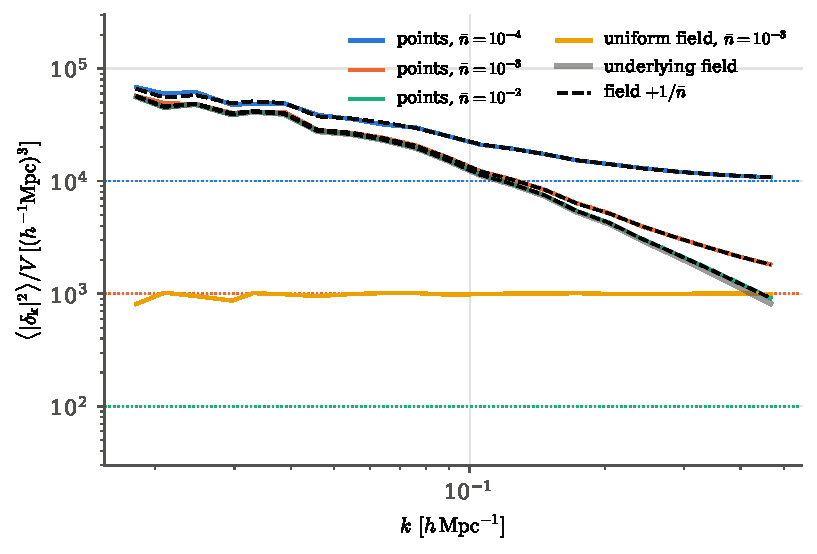
\includegraphics[width=0.78\linewidth]{figures/ch11/poisson_pk.pdf}
\caption{Power spectra of Poisson samples of one lognormal field. The grey band
is the field itself. Each coloured curve is the galaxy power at one mean density,
and the dashed black curves are the field plus $1/\bar n$; the dotted horizontal
lines mark $1/\bar n$. The sparsest sample (blue) is dominated by the flat noise
beyond $k\approx0.1\,h\,\mathrm{Mpc}^{-1}$. The yellow curve is a uniform field
sampled at $\bar n=10^{-3}$: flat at $1000\,h^{-3}\mathrm{Mpc}^3$.}
\label{11a:fig:poisson-pk}
\end{figure}

\Cref{11a:fig:poisson-pk} shows the result. At every density the galaxy power is
the field power lifted by $1/\bar n$, and at $\bar n=10^{-4}$ the lift is so large
that beyond $k\approx0.1\,h\,\mathrm{Mpc}^{-1}$ the galaxies tell us almost
nothing about the field. The power of the sampling noise alone, multiplied by
$\bar n$, averages $\PoisShotA$, $\PoisShotB$ and $\PoisShotC$ at the three
densities, against the predicted $1$; the uniform field gives $\PoisUnif$.

\begin{figure}[htbp]
\centering
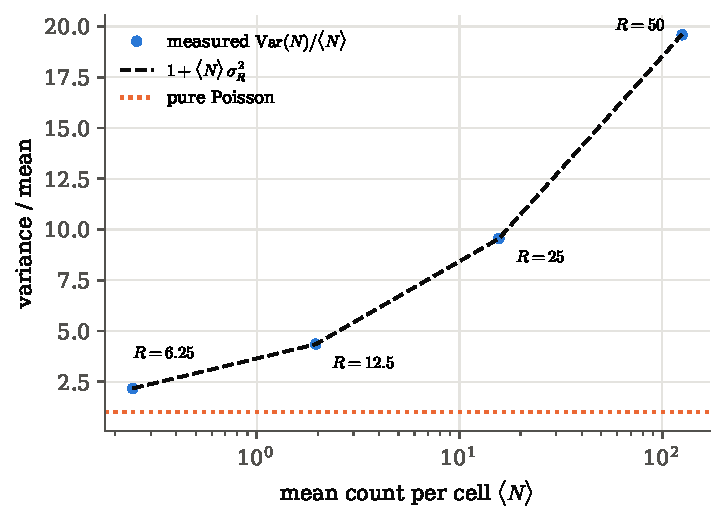
\includegraphics[width=0.62\linewidth]{figures/ch11/poisson_cic.pdf}
\caption{Variance over mean of the counts in cubes of side $R=6.25$ to
$50\,h^{-1}$Mpc, for $\bar n=10^{-3}\,h^3\mathrm{Mpc}^{-3}$. The dots are the
measured ratios, the dashed curve is $1+\bar N\sigma_R^2$ from
\eqref{11a:eq:cic} with $\sigma_R^2$ measured from the field in the same cubes,
and the dotted line is the pure Poisson value $1$.}
\label{11a:fig:poisson-cic}
\end{figure}

\Cref{11a:fig:poisson-cic} checks \eqref{11a:eq:cic}. In the smallest cubes the
measured ratio is $\PoisCicFanoSmall$ against the predicted $\PoisCicPredSmall$;
in the largest, $\PoisCicFanoBig$ against $\PoisCicPredBig$. Both differ from the
prediction by less than the scatter between realisations.

\paragraph{Where the inputs break.}
Each input can fail, and each failure has a signature in the data.
\begin{itemize}[leftmargin=1.2em,itemsep=1pt]
  \item (G2) fails on small scales. Two galaxies cannot overlap, and two massive
        dark matter haloes cannot sit closer than their own radii. That exclusion
        makes counts in small cells \emph{less} variable than Poisson, and the
        effective shot noise smaller than $1/\bar n$ \srcref{Bernardeau2002}{p.~136,
        footnote~60}.
  \item (G2) also fails in the opposite direction. Several galaxies often share
        one halo, so finding one makes another nearby more likely, beyond what
        the smooth field predicts. In the halo model this appears as an extra,
        nearly constant term in $P(k)$ that looks like shot noise but is not
        $1/\bar n$, and the number of galaxies in low-mass haloes is closer to
        binomial than Poisson \cite{CooraySheth2002}. Describing galaxies
        through the haloes they live in is the job of the halo model.
  \item (G1) assumes the rate depends only on the local density. If galaxy
        formation also depends on the environment on larger scales, the relation
        $\delta_g=b\delta$ becomes scale-dependent, which shows up as a bias that
        changes with $k$.
\end{itemize}
In practice the measured shot noise of a sample is a free parameter of the fit,
allowed to differ from $1/\bar n$ by tens of percent. On the scales of the
acoustic peak, where the following sections work, the Cox model is an excellent
description.
\section{Estimating the correlation function from pair counts}
\label{11a:sec:xi}

A survey is never a periodic box. The Sloan footprint is an irregular patch of
sky with holes cut out around bright stars, the galaxy density falls with
distance because faint galaxies drop out, and the edges are wherever the
telescope stopped. The pair probability \eqref{11a:eq:pair-prob} of
\cref{11a:sec:cox} tells us what to measure: count the pairs of galaxies at
separation $r$, and compare with the number we would have found if the galaxies
had no clustering at all. The difficulty is the comparison. In this oddly shaped
survey, with its holes and its falling density, how many pairs at separation $r$
would an \emph{unclustered} set of galaxies have produced? Near an edge a galaxy
has fewer partners at large $r$ simply because part of its surroundings was never
observed, and that loss has nothing to do with cosmology.

Nobody computes that number analytically for a real survey. Instead we
\emph{simulate} it: scatter a large number of points uniformly through the same
survey volume, with exactly the same angular mask and the same fall-off with
distance, and count their pairs. Such a set of points is a \newterm{random
catalogue}. It is Monte Carlo integration (\cref{ch:06}) of the survey's pair
geometry. The rest of the section asks how best to combine the galaxy--galaxy,
galaxy--random and random--random pair counts. Four combinations are in use, and
they behave very differently near edges; the reason fits in one expansion.

\subsection{Pair counts and four estimators}
\label{11a:sec:xi-estimators}

Let the data catalogue hold $N_d$ galaxies and the random catalogue $N_r$ points.
For a separation bin $[r,r+\Delta r)$ define the \newterm{normalised pair counts}
\begin{equation}
\begin{gathered}
  DD(r)=\frac{\#\{\text{ordered galaxy pairs in the bin}\}}{N_d(N_d-1)},\qquad
  DR(r)=\frac{\#\{\text{galaxy--random pairs in the bin}\}}{N_dN_r},\\[2pt]
  RR(r)=\frac{\#\{\text{ordered random pairs in the bin}\}}{N_r(N_r-1)} .
\end{gathered}
  \label{11a:eq:dd-dr-rr}
\end{equation}
Each is the fraction of all possible pairs of its kind that fall in the bin.
Dividing by the number of possible pairs makes the three comparable even though
$N_r$ is several times $N_d$.

\begin{workdef}[pair-count estimators of $\xi(r)$]
With $DD$, $DR$, $RR$ as in \eqref{11a:eq:dd-dr-rr} \unpack{fractions of all
possible pairs that fall in the separation bin},
\begin{align*}
  \hat\xi_{\mathrm N}&=\frac{DD}{RR}-1 &&\text{natural \cite{PeeblesHauser1974}},&
  \hat\xi_{\mathrm{DP}}&=\frac{DD}{DR}-1 &&\text{Davis--Peebles \cite{DavisPeebles1983}},\\
  \hat\xi_{\mathrm H}&=\frac{DD\,RR}{DR^2}-1 &&\text{Hamilton \cite{Hamilton1993}},&
  \hat\xi_{\mathrm{LS}}&=\frac{DD-2DR+RR}{RR} &&\text{Landy--Szalay \cite{LandySzalay1993}}.
\end{align*}
\emph{Operationally:} build a random catalogue with the survey's mask and
selection, count the three kinds of pairs in each bin with a tree code, and
combine.
\end{workdef}

All four are motivated by the same idea. In an unclustered survey $DD$, $DR$ and
$RR$ would agree on average, because galaxies and randoms would then be samples
of the same distribution. Clustering raises $DD$ above the other two by the
factor $1+\xi$. The estimators differ only in which of the noisy, edge-affected
counts they divide by, and that turns out to matter a great deal.

\begin{figure}[htbp]
\centering
\begin{tikzpicture}[scale=1.0]
  \fill[formblue!6] (0,0) rectangle (7,4);
  \draw[bdry] (0,0) rectangle (7,4);
  \fill[white] (5.2,2.6) circle (0.55);
  \draw[bdry] (5.2,2.6) circle (0.55);
  \fill[fibreorange] (2.3,2.0) circle (2pt);
  \draw[tangentgreen,thick] (2.3,2.0) circle (1.2);
  \draw[tangentgreen,thick] (2.3,2.0) circle (1.45);
  \node[lbl,anchor=east] at (2.2,2.0) {$A$};
  \fill[fibreorange] (6.6,0.5) circle (2pt);
  \begin{scope}
    \clip (0,0) rectangle (7,4);
    \draw[tangentgreen,thick] (6.6,0.5) circle (1.2);
    \draw[tangentgreen,thick] (6.6,0.5) circle (1.45);
  \end{scope}
  \begin{scope}
    \clip (7,-1.2) rectangle (8.4,2.2) (5,-1.2) rectangle (7,0);
    \draw[tangentgreen,thick,dashed] (6.6,0.5) circle (1.2);
    \draw[tangentgreen,thick,dashed] (6.6,0.5) circle (1.45);
  \end{scope}
  \node[lbl,anchor=east] at (6.5,0.5) {$B$};
  \foreach \x/\y in {0.6/3.3,1.1/0.7,3.5/3.1,3.9/0.9,4.6/1.8,5.9/3.5,1.5/2.9,3.0/1.4,4.2/2.6,6.2/1.9}
     {\fill[fibreorange] (\x,\y) circle (1.6pt);}
  \foreach \x/\y in {0.4/1.5,0.9/2.3,1.8/0.4,2.7/3.6,3.3/0.3,3.8/2.2,4.5/3.6,4.9/0.6,5.6/1.2,6.4/3.0,
                     1.4/1.5,2.9/2.8,4.1/1.3,5.0/3.3,6.0/0.9,0.5/0.4,2.0/3.5,3.6/1.7,5.9/2.4,6.8/3.6}
     {\draw[softgray] (\x-0.06,\y-0.06) -- (\x+0.06,\y+0.06) (\x-0.06,\y+0.06) -- (\x+0.06,\y-0.06);}
  \node[lbl,bdryred,anchor=north west] at (0,-0.1) {survey edge};
  \node[lbl,bdryred,anchor=west] at (5.8,3.25) {hole};
\end{tikzpicture}
\caption{Why edges matter. Orange dots are galaxies, grey crosses are random
points, the blue region is the observed survey and the red curves are its
boundary. Galaxy $A$ sits in the interior: its whole shell of separations
$[r,r+\Delta r)$ (the green annulus) is observed. Galaxy $B$ sits in a corner:
most of its shell (dashed) lies outside the survey, so it contributes few pairs at
this separation whatever the clustering. Random points near $B$ lose the same
fraction of their shell, which is what the random catalogue is for.}
\label{11a:fig:edges}
\end{figure}

\subsection{What each estimator does to first order}
\label{11a:sec:xi-expansion}

To compare the estimators we write every count as its noise-free value plus a
fluctuation, and keep track of which fluctuations survive in each combination.
This is the calculation of \cite{LandySzalay1993}, set out here in one notation
for all four estimators.

\emph{The fields.} Let $W(\bm x)$ be the survey window, $1$ inside the observed
region and $0$ outside, and $A=\int W\,\dd\bm x$ its area (or volume). The galaxy
number density, smoothed over a scale much smaller than the bin, is
$n_d(\bm x)=(N_d/A)\,W(\bm x)\,[1+\delta_d(\bm x)]$. This defines the
\newterm{data fluctuation} $\delta_d$, which holds the clustering, the Poisson
noise of the sampling, and nothing else. Because the normalisation uses the
actual number $N_d$, the window average of $\delta_d$ is exactly zero:
$\int W\delta_d\,\dd\bm x=0$. The randoms are written the same way, with a
fluctuation $\delta_r$ that holds only their own Poisson noise.

\emph{The pair geometry.} Let $\Theta(\bm x,\bm y)$ be $1$ when
$\abs{\bm x-\bm y}$ falls in the bin and $0$ otherwise, and let
\begin{equation*}
  G=\frac{1}{A^2}\int\!\!\int W(\bm x)W(\bm y)\Theta(\bm x,\bm y)\,\dd\bm x\,\dd\bm y
\end{equation*}
be the fraction of all pairs of points in the survey that fall in the bin. For any
two functions $u$, $v$ write the \newterm{pair average}
\begin{equation*}
  [u\,v]=\frac{1}{A^2G}\int\!\!\int W(\bm x)W(\bm y)\Theta(\bm x,\bm y)\,
  u(\bm x)\,v(\bm y)\,\dd\bm x\,\dd\bm y ,
\end{equation*}
and the \newterm{bin-weighted mean} $a_d=[\delta_d\,1]$, which is the average of
$\delta_d$ over all pair members in the bin; $a_r=[\delta_r\,1]$ likewise.

The counts are then pair averages of products of densities (the self-pairs do not
enter, since $r>0$):
\begin{align}
  DD&\eqby{1}\frac{1}{A^2}\int\!\!\int WW\Theta\,(1+\delta_d)(1+\delta_d)
     \eqby{2} G\bigl(1+2a_d+[\delta_d\delta_d]\bigr),\nonumber\\
  DR&\eqby{3} G\bigl(1+a_d+a_r+[\delta_d\delta_r]\bigr),\qquad
  RR\eqby{4} G\bigl(1+2a_r+[\delta_r\delta_r]\bigr).
  \label{11a:eq:counts-expanded}
\end{align}
\begin{explain}
  \item The fraction of galaxy pairs in the bin is the pair integral of the
        normalised density $n_d/(N_d/A)=W(1+\delta_d)$ at both ends.
  \item Multiply out: the $1\cdot1$ term gives $G$; the two cross terms are each
        $G\,a_d$, by symmetry of $\Theta$; the last is $G[\delta_d\delta_d]$.
  \item The same with $1+\delta_r$ at one end.
  \item The same with $1+\delta_r$ at both ends.
\end{explain}

The first-order quantities are $a_d$ and $a_r$; the pair averages
$[\delta\,\delta]$ are second order. The one we want is $[\delta_d\delta_d]$,
whose expectation is $\xi(r)$ up to the small correction derived below. Now
insert \eqref{11a:eq:counts-expanded} into each estimator and expand to first
order in $a_d$, $a_r$, keeping the second-order pair averages:
\begin{align}
  \hat\xi_{\mathrm N}
  &\eqby{1}\frac{1+2a_d+[\delta_d\delta_d]}{1+2a_r+[\delta_r\delta_r]}-1
   \approx [\delta_d\delta_d]-[\delta_r\delta_r]+2(a_d-a_r),\nonumber\\
  \hat\xi_{\mathrm{DP}}
  &\eqby{2}\frac{1+2a_d+[\delta_d\delta_d]}{1+a_d+a_r+[\delta_d\delta_r]}-1
   \approx [\delta_d\delta_d]-[\delta_d\delta_r]+(a_d-a_r),\nonumber\\
  \hat\xi_{\mathrm H}
  &\eqby{3}\frac{(1+2a_d+[\delta_d\delta_d])(1+2a_r+[\delta_r\delta_r])}
     {(1+a_d+a_r+[\delta_d\delta_r])^2}-1
   \approx \bigl[(\delta_d-\delta_r)(\delta_d-\delta_r)\bigr]-(a_d-a_r)^2,\nonumber\\
  \hat\xi_{\mathrm{LS}}
  &\eqby{4}\frac{[\delta_d\delta_d]-2[\delta_d\delta_r]+[\delta_r\delta_r]}
   {1+2a_r+[\delta_r\delta_r]}
   =\frac{\bigl[(\delta_d-\delta_r)(\delta_d-\delta_r)\bigr]}{1+2a_r+[\delta_r\delta_r]}.
  \label{11a:eq:estimators-expanded}
\end{align}
\begin{explain}
  \item The common factor $G$ cancels; to first order $1/(1+\epsilon)\approx1-\epsilon$.
  \item The same, with $DR$ in the denominator: the first-order terms are
        $2a_d-(a_d+a_r)=a_d-a_r$.
  \item Keeping only the $a$'s, the numerator minus the denominator is
        $1+2a_d+2a_r+4a_da_r-(1+a_d+a_r)^2=-(a_d-a_r)^2$: the first-order terms
        cancel identically. The pair averages enter as
        $[\delta_d\delta_d]+[\delta_r\delta_r]-2[\delta_d\delta_r]$.
  \item In $DD-2DR+RR$ every term of $G(1+\dots)$ that is zeroth or first order
        cancels: $1-2+1=0$ and $2a_d-2(a_d+a_r)+2a_r=0$. What is left is the pair
        average of the product of the two \emph{differences} $\delta_d-\delta_r$.
\end{explain}

So the natural estimator carries the first-order term $2(a_d-a_r)$, the
Davis--Peebles estimator carries half of it, and the Hamilton and Landy--Szalay
estimators carry none. What is $a_d$, physically? It is the average of the data
fluctuation over the members of all pairs in the bin. Every point of the survey
is weighted by the fraction of its shell that lies inside the survey. Interior
points (like $A$ in \cref{11a:fig:edges}) get full weight; points near an edge
(like $B$) get less. The plain survey average of $\delta_d$ is zero by
construction, but this \emph{edge-weighted} average is not. If the interior of
the survey happens to be overdense and the edges underdense, $a_d$ is positive.
It is a large-scale fluctuation, of first order in $\delta$, and at the
separations where $\xi$ is small it is far larger than the signal.

\begin{keyidea}[Why Landy--Szalay wins]
The Landy--Szalay numerator is the pair average of
$(\delta_d-\delta_r)(\delta_d-\delta_r)$: the product of the data fluctuation and
the random fluctuation at the two ends of each pair. It contains no term linear
in either fluctuation, so the edge-weighted large-scale fluctuations $a_d$ and
$a_r$ that dominate the error of $DD/RR-1$ and $DD/DR-1$ at large separations
cancel exactly. What remains is the scatter of the pair average itself, which no
pair-count estimator can avoid.
\end{keyidea}

In the weak-correlation limit Landy and Szalay showed that this residual scatter
is just the Poisson scatter of the pair counts, the smallest possible, while the
variances of $DD/RR$ and $DD/DR$ are considerably larger than Poisson
\srcref{LandySzalay1993}{\S4}. The Hamilton estimator also cancels the
first-order term, only through a product rather than a difference, and it
performs almost as well; a systematic comparison of nine estimators on large
simulations ranks the two together at the top \cite{Kerscher2000}
\srcref{Bernardeau2002}{\S6.4.1, p.~139}.

\paragraph{How much does the edge term cost?}
The claim that LS reaches the smallest scatter can be checked in the simplest
case, where both errors can be computed by hand: galaxies with no clustering at
all ($\xi=0$), and a random catalogue so large that its own noise vanishes
($\delta_r=0$, so $a_r=0$). Then LS reduces to $[\delta_d\delta_d]$ and the
natural estimator to $[\delta_d\delta_d]+2a_d$. Two questions remain. How much
does the pair average $[\delta_d\delta_d]$ scatter? And how much does $a_d$?

\emph{The pair term.} The bin contains on average
$N_p=\tfrac12N_d^2G$ distinct galaxy pairs. With no clustering, whether a given
pair lands in the bin is a rare event that hardly depends on the other pairs, so
the count of pairs scatters like a Poisson count (\cref{2a:sec:poisson-inputs}),
with fractional standard deviation $N_p^{-1/2}$. Since
$DD=G(1+[\delta_d\delta_d])$ when $a_d$ is set aside, that fractional scatter is
the scatter of $[\delta_d\delta_d]$: its variance is $1/N_p$.

\emph{The edge term.} Write $e(\bm x)$ for the fraction of the survey that lies in
the shell around $\bm x$, divided by its average over the survey; $e=1$ on
average, $e<1$ near edges and holes. Then
\begin{align}
  a_d&\eqby{1}\frac{1}{A}\int W(\bm x)\,\delta_d(\bm x)\,e(\bm x)\,\dd\bm x
     \eqby{2}\frac{1}{N_d}\sum_{i=1}^{N_d}e(\bm x_i)-1,\nonumber\\
  \Var(a_d)&\eqby{3}\frac{\sigma_e^2}{N_d},
  \qquad \sigma_e^2=\frac1A\int W\,(e-1)^2\,\dd\bm x .
  \label{11a:eq:ad-variance}
\end{align}
\begin{explain}
  \item In the definition of $a_d=[\delta_d\,1]$, do the integral over the partner
        $\bm y$ first: it gives the area of $\bm x$'s shell inside the survey,
        which is $A\,G\,e(\bm x)$ by the definitions of $e$ and of $G$.
  \item Replace $W\delta_d$ by $(A/N_d)\,n_d-W$, from the definition of
        $\delta_d$. The density $n_d$ is a sum of spikes at the galaxies, so its
        integral against $e$ is $\sum_ie(\bm x_i)$; the integral of $We$ is $A$,
        since $e$ averages to $1$.
  \item Unclustered galaxies are $N_d$ independent uniform points in the
        survey, so the $e(\bm x_i)$ are independent with mean $1$ and variance
        $\sigma_e^2$; the variance of their mean is $\sigma_e^2/N_d$.
\end{explain}
So $a_d$ is simply the average edge weight of the galaxies we happened to get,
minus its expected value. Comparing the two contributions to the natural
estimator,
\begin{equation}
  \frac{\Var(2a_d)}{\Var([\delta_d\delta_d])}
  =\frac{4\sigma_e^2/N_d}{1/N_p}
  =2\,\sigma_e^2\,N_dG .
  \label{11a:eq:edge-vs-pairs}
\end{equation}
The product $N_dG$ is the average number of neighbours a galaxy has in the bin.
For a square survey of side $700\,h^{-1}$Mpc and $r=100\,h^{-1}$Mpc, a direct
numerical average of the shell fraction over the square gives
$\sigma_e^2\approx0.064$. A galaxy with $1000$ neighbours in the bin then makes the
edge term $\approx130$ times the pair noise in variance, about eleven times in
standard deviation. LS removes that term and keeps only the $1/N_p$ that no
pair-count estimator can avoid. In a periodic box $e=1$ everywhere, so
$\sigma_e^2=0$ and the edge term is absent from every estimator.

\paragraph{Example: a periodic box.}
In a periodic box there are no edges: every point has its whole shell inside the
box, so the edge weighting is uniform and $a_d$ equals the plain average of
$\delta_d$, which is zero. The same holds for $a_r$. The first-order terms of the
natural and Davis--Peebles estimators then vanish, and all four estimators are
equivalent to first order. Simulations of a periodic box should show four nearly
identical scatters; any difference must come from the survey's edges.

\paragraph{Example: how big is the edge weight?}
Take a square survey of side $700\,h^{-1}$Mpc and $r=100\,h^{-1}$Mpc. A point at
the centre has its whole shell inside. A point in a corner has a quarter of it. A point on an edge, away from the corners, has exactly half: a straight
edge through the centre of a circle cuts it into two equal halves. So the edge weight varies by a factor of
four across the survey. Within $100\,h^{-1}$Mpc of the boundary lies a fraction
$1-(500/700)^2\approx0.49$ of the area: half of the survey's galaxies take part
in pairs with reduced weight. If that outer half happens to be $1\%$ underdense,
which is typical of fluctuations on scales of hundreds of Mpc, then $a_d$ is of order
$10^{-3}$, a sizeable fraction of $\xi$ itself at $r=100\,h^{-1}$Mpc, which is a few $\times10^{-3}$.

\paragraph{Example: how many randoms?}
The random catalogue's own Poisson noise enters through $\delta_r$. In the natural
estimator it appears at first order, through $-2a_r$, whose variance falls only
as $1/N_r$; so the natural estimator needs a random catalogue far larger than
the data to be competitive. In Landy--Szalay $\delta_r$ enters only through the
difference $\delta_d-\delta_r$, inside a product, and a random catalogue a few
times larger than the data is enough. Eisenstein and collaborators used at least
sixteen times as many randoms as galaxies \srcref{Eisenstein2005}{\S3.1}; our
simulation uses five.

\subsection{The integral constraint}
\label{11a:sec:integral-constraint}

Removing the first-order terms does not remove every bias. The trouble is the
normalisation by the observed $N_d$. In a survey that happens to be overdense as a
whole, dividing by the observed mean density makes the survey look average, and
pairs everywhere look less correlated than they are. We can say how much less.

Write the true field as $\delta$ and its plain survey average as
$\bar\delta_W=\frac1A\int W\delta\,\dd\bm x$. Leaving out the Poisson noise, which
does not correlate distinct points (\cref{11a:sec:cox-moments}), the normalised
data fluctuation is $1+\delta_d=(1+\delta)/(1+\bar\delta_W)$, so
$\delta_d\approx\delta-\bar\delta_W$ to first order. Then
\begin{align}
  \E\bigl[\,[\delta_d\delta_d]\,\bigr]
  &\eqby{1}\E\bigl[\,[(\delta-\bar\delta_W)(\delta-\bar\delta_W)]\,\bigr]
   \eqby{2}\E\bigl[[\delta\delta]\bigr]-2\,\E\bigl[[\delta\,1]\,\bar\delta_W\bigr]
     +\E\bigl[\bar\delta_W^2\bigr]\nonumber\\
  &\eqby{3}\xi(r)-2\,\E\bigl[[\delta\,1]\,\bar\delta_W\bigr]+\bar\xi
   \eqby{4}\xi(r)-\bar\xi,
  \qquad
  \bar\xi\equiv\frac{1}{A^2}\int\!\!\int W(\bm x)W(\bm y)\,\xi(\abs{\bm x-\bm y})\,
  \dd\bm x\,\dd\bm y . \label{11a:eq:ic}
\end{align}
\begin{explain}
  \item $\delta_d\approx\delta-\bar\delta_W$.
  \item Multiply out the product; $\bar\delta_W$ is a number, the same at both
        ends of every pair, and $[1\,1]=1$.
  \item The expectation of $\delta(\bm x)\delta(\bm y)$ is $\xi$ at their
        separation, which is fixed within the bin; $\E[\bar\delta_W^2]$ is the
        double window average of $\xi$, called $\bar\xi$.
  \item $\E\bigl[[\delta\,1]\,\bar\delta_W\bigr]$ is the average of $\xi$ between a
        pair member and a random point of the survey. Ignoring the edge weighting
        it equals $\bar\xi$ as well, and $-2\bar\xi+\bar\xi=-\bar\xi$.
\end{explain}
All four estimators share this bias, because all of them normalise by the
observed number of galaxies. It is called the \newterm{integral constraint}: the
measured correlation function, integrated over the survey, is forced to be
close to zero, because the survey's own mean density was taken as the truth. It
shifts $\hat\xi$ down by the constant $\bar\xi$, the variance of the mean density
of the survey, and it cannot be removed by any combination of pair counts, only
modelled \srcref{Bernardeau2002}{eq.~(393) and p.~141}. At small separations,
where $\xi\gg\bar\xi$, it is negligible; at the scale of the acoustic peak it is
not. A commonly used form that also holds when $\xi$ is not small is
$\E[\hat\xi]\approx(1+\xi)/(1+\bar\xi)-1$, which reduces to $\xi-\bar\xi$ to
first order.

\begin{pitfall}[The randoms must have the survey's selection, exactly]
Every estimator derivation so far assumes that the randoms are a uniform sample of
the \emph{same} window as the data, including the fall-off of density with
distance and every masked region. If the randoms are a little too dense in one
part of the survey (an error in the photometric calibration of one patch of sky,
say), then $\delta_d$ acquires a large-scale pattern that is not cosmology, and
its pair average adds a spurious $\xi$ at every separation. Eisenstein and
collaborators found that a $1\%$ shift in the $r-i$ colour changes the LRG
number density by $8$--$10\%$ \srcref{Eisenstein2005}{\S3.2}. Real analyses spend
much of their effort building the random catalogue and its weights.
\end{pitfall}

\subsection{Testing the estimators in a survey with holes}
\label{11a:sec:xi-python}

The script \pyname{code/ch11/02_xi_estimators.py} makes the question concrete in
two dimensions, where pair counts are cheap. The field is a lognormal field
(\cref{11a:sec:lognormal}) of unit variance on a grid of $256^2$ cells in a box of
side $1000\,h^{-1}$Mpc; its two-point function is known exactly on the grid, and
it is $\XiTrueMid$ at $r=\XiRmid\,h^{-1}$Mpc and $\XiTrueBig$ at
$r=\XiRbig\,h^{-1}$Mpc. The survey window is a $700\times700$ square with five
circular holes and a notch, of area $\XiArea\times10^3\,h^{-2}\mathrm{Mpc}^2$
(\cref{11a:fig:xi-survey}). Each of $\XiNsim$ mock catalogues is a Poisson sample
with $\bar n=\XiNbar\,h^2\mathrm{Mpc}^{-2}$ inside the window, about $\XiNg$
galaxies, and each mock gets its own random catalogue of $\XiNr$ points.

\begin{figure}[htbp]
\centering
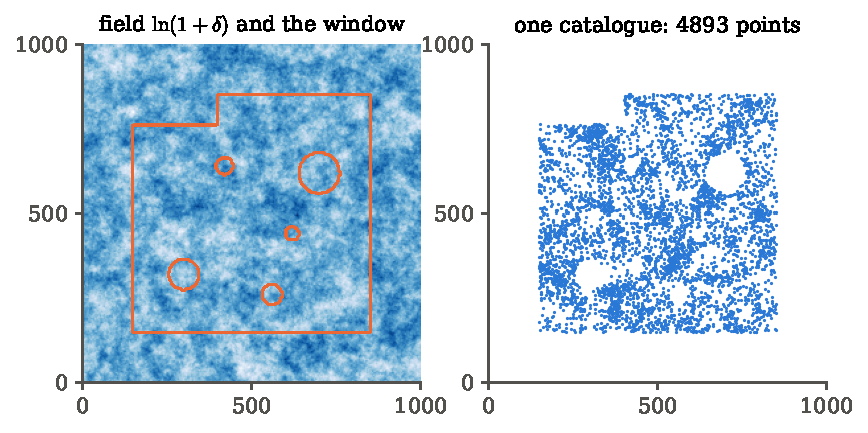
\includegraphics[width=0.8\linewidth]{figures/ch11/xi_survey.pdf}
\caption{The test survey. Left: one lognormal field (shown as $\ln(1+\delta)$)
with the survey boundary and holes in orange. Right: one Poisson catalogue drawn
from a field inside that window.}
\label{11a:fig:xi-survey}
\end{figure}

\pyfile[firstline=64,lastline=101,firstnumber=64]{code/ch11/02_xi_estimators.py}{Pair counts and the four estimators}

\pyname{counts} uses \pyname{cKDTree.count_neighbors}, which returns, for each
bin edge, the number of ordered pairs closer than that edge; differencing gives
the pairs per bin. A tree visits only nearby branches, so the cost grows much more
slowly than the $N^2$ of a double loop. Lines~73, 93 and~95 divide by the numbers of
possible pairs, \eqref{11a:eq:dd-dr-rr}, and line~80 forms the four estimators.
The same estimators are also computed in a periodic box with the same number of
points and no edges, as the control of the first example above. Finally, the
integral constraint $\bar\xi$ of \eqref{11a:eq:ic} is evaluated exactly on the
grid (lines~56--58 of the script) by a Fourier transform: the double window
integral is the window's autocorrelation times $\xi$, summed. It is
$\bar\xi=\XiBar$ for this window.

\begin{figure}[htbp]
\centering
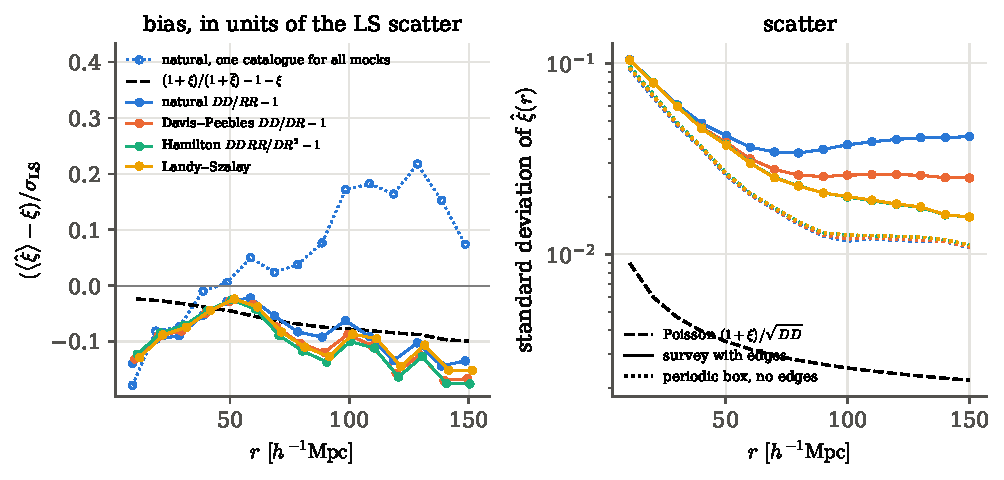
\includegraphics[width=0.95\linewidth]{figures/ch11/xi_estimators.pdf}
\caption{The four estimators over $\XiNsim$ mock surveys. Left: the mean minus
the true $\xi(r)$, in units of the Landy--Szalay scatter; the dashed curve is the
integral-constraint expectation $(1+\xi)/(1+\bar\xi)-1-\xi$; the open circles are the natural
estimator when one random catalogue is reused for every mock. Right: the standard
deviation of each estimator in the survey with holes (solid) and in a periodic
box with the same number of points (dotted), with the Poisson floor
$(1+\xi)/\sqrt{DD}$ (dashed black).}
\label{11a:fig:xi-estimators}
\end{figure}

\Cref{11a:fig:xi-estimators} answers the question. On the right, in the survey
with holes, the natural estimator's scatter at $r=\XiRbig\,h^{-1}$Mpc is
$\XiRatioNatBig$ times that of Landy--Szalay, Davis--Peebles is $\XiRatioDPBig$
times, and Hamilton is $\XiRatioHamBig$ times: exactly the ordering of the
first-order terms in \eqref{11a:eq:estimators-expanded}, coefficient $2$, $1$, $0$
and $0$. At $r=\XiRmid\,h^{-1}$Mpc, where $\xi$ is large and the first-order
term is relatively unimportant, the ratios shrink to $\XiRatioNatMid$ and
$\XiRatioDPMid$. In the periodic control the four scatters nearly coincide (the
natural-to-LS ratio is $\XiPerRatioNatBig$ at $\XiRbig\,h^{-1}$Mpc): without edges
there is nothing for Landy--Szalay to cancel. On the left, all four means follow the integral-constraint curve. At
$r=\XiRbig\,h^{-1}$Mpc the prediction is $\XiICBig$ (the true $\xi$ is $\XiTrueBig$);
Landy--Szalay gives $\XiMeanLSBig\pm\XiErrMeanBig$, Hamilton $\XiMeanHamBig$,
Davis--Peebles $\XiMeanDPBig$, and the natural estimator $\XiMeanNatBig\pm\XiErrMeanNatBig$.
On average, then, none of them is biased beyond the integral constraint; they differ
in how much they scatter.

That agreement needs one precaution, and it is easy to miss. Suppose we save time and
make a single random catalogue for all $\XiNsim$ mocks. Landy--Szalay and Hamilton do not
notice: their means become $\XiFixLSBig$ and $\XiFixHamBig$. But the natural estimator's
mean moves, in this run to $\XiFixNatBig$, and Davis--Peebles' to $\XiFixDPBig$. How
far they move, and in which direction, depends on which random catalogue happened to
be drawn; another catalogue would shift them by a different amount. The reason is the first-order random term of the previous example. Each random
catalogue has its own small lumps, and the natural estimator carries them straight into
$\hat\xi$. With a fresh catalogue for every mock those lumps differ from mock to mock
and average away. With one shared catalogue they are the same in every mock, so
averaging $\XiNsim$ mocks cannot remove them, and the error bar computed from the
scatter of the mocks does not even know they are there. Landy--Szalay cancels the
random lumps by construction, which is one more reason to prefer it.

Notice also how far the scatter is above the Poisson floor: at
$r=\XiRbig\,h^{-1}$Mpc the LS standard deviation is $\XiSdLSBig$ and the Poisson
floor is $\XiSdPoisBig$. Landy and Szalay's optimality is a statement about the
noise their estimator \emph{adds}. The scatter that remains is mostly the sample
variance of the field: the survey holds only a few independent patches of size
$100\,h^{-1}$Mpc, and the field in those patches is one draw. No estimator removes
that; only a bigger survey does.
\section{The power spectrum of a survey: the FKP estimator}
\label{11a:sec:fkp}

A flux-limited survey is dense nearby and sparse far away. Close to us we see
faint galaxies as well as bright ones, so the mean density $\bar n(\bm x)$ is high;
at the far edge only the most luminous galaxies make it into the catalogue, and
$\bar n$ may be a hundred times lower. Both parts of the survey carry information
about $P(k)$, but of different quality. The nearby part is limited by its small
volume: it holds few independent Fourier modes, and its error is sample variance.
The distant part has plenty of volume but few galaxies: its error is shot noise.
If we Fourier transform the galaxy density with every galaxy counted equally, the
crowded nearby region dominates the answer and the huge distant volume is wasted.

The question in words: \emph{how much weight should a galaxy get, depending on
where it sits, so that the estimated power spectrum has the smallest possible
error?} Feldman, Kaiser and Peacock answered it in 1994, and the answer, the FKP
weight, is used in essentially every galaxy power-spectrum measurement since
\cite{FKP1994}. Its derivation needs only the Cox model of \cref{11a:sec:cox} and
the Gaussian statistics of Fourier modes from \cref{ch:07}.

\subsection{The weighted field and its mean power}
\label{11a:sec:fkp-mean}

Write the galaxy catalogue as a sum of spikes,
$n_g(\bm x)=\sum_i\delta_D(\bm x-\bm x_i)$, and do the same for a random catalogue
with the same selection but $1/\alpha$ times as many points, $n_s(\bm x)$. Here
$\bar n(\bm x)$ is the expected galaxy density at $\bm x$ in the absence of
clustering, set by the survey's angular mask and its fall-off with distance, and
$w(\bm x)$ is a weight still to be chosen. FKP's weighted fluctuation field is
\begin{equation}
  F(\bm x)=\frac{w(\bm x)\,\bigl[n_g(\bm x)-\alpha\,n_s(\bm x)\bigr]}{I^{1/2}},
  \qquad I=\int\bar n^2(\bm x)\,w^2(\bm x)\,\dd^3x
  \label{11a:eq:fkp-field}
\end{equation}
\srcref{FKP1994}{eq.~(2.1.3)}. The randoms subtract the mean density, so $F$ is
zero on average; the weight shapes how much each place counts; and $I$ is chosen
so that $\E|F_{\bm k}|^2$ comes out, in the calculation below, as $P(k)$ itself.

The two-point functions of the catalogues follow from \cref{11a:sec:cox-moments},
now with a mean density that varies with position. For galaxies, the pair term
\eqref{11a:eq:pair-count} becomes $\bar n(\bm x)\bar n(\bm y)[1+\xi(\bm x-\bm y)]$,
and the Poisson variance of a single cell, $\bar n\Delta V$, becomes the self-pair
spike $\bar n(\bm x)\delta_D(\bm x-\bm y)$ in the continuum. Randoms are an
unclustered Cox sample with density $\bar n/\alpha$, independent of the galaxies:
\begin{equation}
\begin{aligned}
  \E[n_g(\bm x)n_g(\bm y)]&=\bar n(\bm x)\bar n(\bm y)\bigl[1+\xi(\bm x-\bm y)\bigr]
     +\bar n(\bm x)\,\delta_D(\bm x-\bm y),\\
  \E[n_s(\bm x)n_s(\bm y)]&=\alpha^{-2}\bar n(\bm x)\bar n(\bm y)
     +\alpha^{-1}\bar n(\bm x)\,\delta_D(\bm x-\bm y),\qquad
  \E[n_g(\bm x)n_s(\bm y)]=\alpha^{-1}\bar n(\bm x)\bar n(\bm y)
\end{aligned}
  \label{11a:eq:fkp-twopoint}
\end{equation}
\srcref{FKP1994}{eq.~(2.1.5)}. With the Fourier convention
$F_{\bm k}=\int F(\bm x)e^{-i\bm k\cdot\bm x}\dd^3x$, so that an infinite field
has $\E[\delta_{\bm k}\delta^*_{\bm k'}]=(2\pi)^3\delta_D(\bm k-\bm k')P(k)$,
\begin{align}
  \E\abs{F_{\bm k}}^2
  &\eqby{1}\frac1I\int\!\!\int w(\bm x)w(\bm y)\,
     \E\bigl[(n_g-\alpha n_s)_{\bm x}(n_g-\alpha n_s)_{\bm y}\bigr]
     e^{-i\bm k\cdot(\bm x-\bm y)}\dd^3x\,\dd^3y\nonumber\\
  &\eqby{2}\frac1I\int\!\!\int w(\bm x)w(\bm y)\Bigl[\bar n(\bm x)\bar n(\bm y)\,
     \xi(\bm x-\bm y)+(1+\alpha)\,\bar n(\bm x)\,\delta_D(\bm x-\bm y)\Bigr]
     e^{-i\bm k\cdot(\bm x-\bm y)}\dd^3x\,\dd^3y\nonumber\\
  &\eqby{3}\int\frac{\dd^3k'}{(2\pi)^3}\,P(k')\,
     \abs{\tilde G(\bm k-\bm k')}^2+P_{\mathrm{shot}},
  \label{11a:eq:fkp-mean}\\
  \tilde G(\bm q)&\equiv\frac{1}{I^{1/2}}\int\bar n(\bm x)w(\bm x)\,
     e^{-i\bm q\cdot\bm x}\,\dd^3x,\qquad
  P_{\mathrm{shot}}\equiv\frac{(1+\alpha)}{I}\int\bar n(\bm x)\,w^2(\bm x)\,\dd^3x .
  \nonumber
\end{align}
\begin{explain}
  \item Square the Fourier transform of \eqref{11a:eq:fkp-field} and take the
        expectation inside the integrals.
  \item Expand the bracket with \eqref{11a:eq:fkp-twopoint}: the four
        $\bar n\bar n$ terms are $1-1-1+1=0$, leaving the clustering term
        $\bar n\bar n\,\xi$; the spikes come in with coefficients $1$ (galaxies)
        and $\alpha^2\cdot\alpha^{-1}=\alpha$ (randoms).
  \item In the first term write $\xi(\bm x-\bm y)=\int\frac{\dd^3k'}{(2\pi)^3}P(k')
        e^{i\bm k'\cdot(\bm x-\bm y)}$; the $\bm x$ and $\bm y$ integrals then
        factorise into $\tilde G(\bm k-\bm k')$ and its complex conjugate. In the
        second term the spike sets $\bm y=\bm x$ and the exponential becomes $1$.
\end{explain}
The first term is the true spectrum blurred by the window. The function
$\abs{\tilde G}^2$ is the power spectrum of the weighted survey shape
$\bar nw$; for a survey of size $D$ it is a blob of width about $1/D$ around
$\bm q=0$, and by Parseval's theorem its integral
$\int\frac{\dd^3q}{(2\pi)^3}\abs{\tilde G}^2=\frac1I\int\bar n^2w^2\,\dd^3x=1$. So
on scales much smaller than the survey, $k\gg1/D$, where $P$ hardly changes across
the blob, \eqref{11a:eq:fkp-mean} becomes
\begin{equation}
  \E\abs{F_{\bm k}}^2\approx P(k)+P_{\mathrm{shot}},\qquad
  \hat P(k)=\frac{1}{V_k}\int_{\text{shell}}\bigl(\abs{F_{\bm k'}}^2-P_{\mathrm{shot}}\bigr)
  \,\dd^3k'
  \label{11a:eq:fkp-estimator}
\end{equation}
\srcref{FKP1994}{eqs.~(2.1.8)--(2.1.11)}, where $V_k$ is the volume of the shell of
wavevectors averaged over. This is the \newterm{FKP estimator}: Fourier transform
the weighted field, square, subtract the known shot noise, average over a shell.

Two corrections are hidden in the ``$\approx$''. On scales comparable to the
survey, $k\sim1/D$, the window convolution in \eqref{11a:eq:fkp-mean} is not
negligible: it smooths out features and suppresses power at the lowest $k$. It is
the same mode coupling met for masked skies in \cref{8b:sec:coupling}, and it is
handled the same way, by convolving the \emph{model} with the window before
comparing it with the data. And the shot noise subtracted is the Poisson value;
\cref{11a:sec:cox} listed why real galaxies need not be exactly Poisson.

\paragraph{Example: a uniform survey.}
For constant $\bar n$ and $w$ inside a volume $V$, $I=\bar n^2w^2V$ and
$P_{\mathrm{shot}}=(1+\alpha)\bar nw^2V/(\bar n^2w^2V)=(1+\alpha)/\bar n$. With a
random catalogue much larger than the data, $\alpha\to0$, and we recover the
$1/\bar n$ of \eqref{11a:eq:shot}. A finite random catalogue adds its own shot
noise, $\alpha/\bar n$: with twenty times as many randoms as galaxies that is a
$5\%$ addition, which is why the randoms are made large.

\subsection{The error, and the weight that minimises it}
\label{11a:sec:fkp-weight}

To choose $w$ we need the variance of $\hat P(k)$. Assume the Fourier modes $F_{\bm
k}$ are Gaussian; for the long-wavelength modes of a survey this is a good
approximation, because each $F_{\bm k}$ is a sum over a huge number of
galaxies (the central limit theorem of \cref{3a:sec:clt}). Write
$C(\bm k,\bm k')=\E[F_{\bm k}F^*_{\bm k'}]$. Repeat the first two steps of
\eqref{11a:eq:fkp-mean}, but keep the two wavevectors different, so that the
phases are $e^{-i\bm k\cdot\bm x+i\bm k'\cdot\bm y}$. The spike term then gives,
after the $\delta_D$ sets $\bm y=\bm x$, the number
$\tilde S(\bm q)=\frac{1+\alpha}{I}\int\bar nw^2e^{-i\bm q\cdot\bm x}\dd^3x$ at
$\bm q=\bm k-\bm k'$. The clustering term, with $\xi$ written as the integral of
$P$ as before, is $\int\frac{\dd^3k''}{(2\pi)^3}P(k'')\,\tilde G(\bm k-\bm k'')\,
\tilde G^*(\bm k'-\bm k'')$. Both $\tilde G$ factors are blobs of width $\sim1/D$,
so only $\bm k''$ within $1/D$ of $\bm k$ contributes, and there $P$ is nearly
the constant $P(k)$. Pulling it out leaves the convolution of $\tilde G$ with its
own conjugate, which is the Fourier transform of $\abs{G(\bm x)}^2=\bar n^2w^2/I$:
that is $\tilde Q(\bm q)$. So
$C(\bm k,\bm k')\approx P(k)\,\tilde Q(\bm k-\bm k')+\tilde S(\bm k-\bm k')$
\srcref{FKP1994}{eqs.~(2.2.2)--(2.2.5)}, with $\tilde Q$ the Fourier transform of
$\bar n^2w^2/I$. Both $\tilde Q$ and $\tilde S$ are blobs of width $\sim1/D$ around
zero, and the covariance of two modes dies away once they are more than $1/D$
apart. Then
\begin{align}
  \Var\hat P(k)
  &\eqby{1}\frac{1}{V_k^2}\int_{\text{shell}}\!\int_{\text{shell}}
     \Bigl[\abs{C(\bm k,\bm k')}^2+\abs{C(\bm k,-\bm k')}^2\Bigr]
     \dd^3k\,\dd^3k'\nonumber\\
  &\eqby{2}\frac{2}{V_k}\int\abs{P\,\tilde Q(\bm q)+\tilde S(\bm q)}^2\,\dd^3q
   \eqby{3}\frac{2(2\pi)^3}{V_k\,I^2}\int\bigl[\bar n^2w^2P+(1+\alpha)\bar nw^2\bigr]^2\dd^3x,
  \nonumber\\
  \frac{\Var\hat P(k)}{P^2(k)}
  &\eqby{4}\frac{2(2\pi)^3}{V_k}\,
   \frac{\int\bar n^4w^4\bigl[1+1/(\bar nP)\bigr]^2\dd^3x}
        {\bigl[\int\bar n^2w^2\,\dd^3x\bigr]^2}.
  \label{11a:eq:fkp-var}
\end{align}
\begin{explain}
  \item The covariance of $\abs{F_{\bm k}}^2$ and $\abs{F_{\bm k'}}^2$ for complex
        Gaussian modes, by Isserlis' theorem (\cref{7a:sec:grf-predicts}). The
        second term is there because the field is real, $F_{-\bm k'}=F^*_{\bm k'}$,
        so a mode near $-\bm k$ is the same mode as one near $\bm k$.
  \item $C$ depends only on $\bm q=\bm k-\bm k'$ and is narrow compared with the
        shell, so for each $\bm k$ the $\bm k'$ integral covers the whole blob; the
        remaining $\bm k$ integral gives $V_k$. The second term gives the same.
  \item Parseval: $\int\abs{\tilde g(\bm q)}^2\dd^3q=(2\pi)^3\int\abs{g(\bm x)}^2\dd^3x$,
        with $g=[\bar n^2w^2P+(1+\alpha)\bar nw^2]/I$.
  \item Divide by $P^2$, take $\alpha\to0$, and insert $I=\int\bar n^2w^2$.
\end{explain}
This is FKP's eq.~(2.3.2), up to the factor~$2$.\footnote{FKP keep only the
neighbourhood $\bm k'\approx\bm k$ in their eq.~(2.3.1). For a real field the
neighbourhood $\bm k'\approx-\bm k$ is the same set of modes counted again, which
doubles the variance, as in the mode counting of
\srcref{SeoEisenstein2003}{eq.~(8)}. The factor does not change the optimal
weight.}

Now the question becomes a small optimisation problem. Write $u=\bar n^2w^2\ge0$
and $c=1+1/(\bar nP)$. The fractional variance is proportional to
$R[u]=\int u^2c^2/\bigl(\int u\bigr)^2$, and we want the $u$ that makes it
smallest. The Cauchy--Schwarz inequality does it in one line:
\begin{align}
  \Bigl(\int u\,\dd^3x\Bigr)^2
  &\eqby{1}\Bigl(\int (u\,c)\,\frac1c\,\dd^3x\Bigr)^2
   \relby{2}{\le}\int u^2c^2\,\dd^3x\;\int\frac{1}{c^2}\,\dd^3x,\nonumber\\
  R[u]&\relby{3}{\ge}\frac{1}{\int c^{-2}\,\dd^3x}
   \eqby{4}\frac{1}{\int\bigl[\frac{\bar nP}{1+\bar nP}\bigr]^2\dd^3x}.
  \label{11a:eq:fkp-cs}
\end{align}
\begin{explain}
  \item Multiply and divide by $c>0$.
  \item Cauchy--Schwarz for integrals,
        $\bigl(\int fg\bigr)^2\le\int f^2\int g^2$, with $f=uc$ and $g=1/c$.
        Equality holds exactly when $f\propto g$.
  \item Divide both sides by $(\int u)^2\int c^{-2}$.
  \item $1/c=\bar nP/(1+\bar nP)$.
\end{explain}
The bound is reached when $uc\propto1/c$, that is $\bar n^2w^2\propto
[\bar nP/(1+\bar nP)]^2$, or
\begin{equation}
  w_{\mathrm{FKP}}(\bm x)=\frac{1}{1+\bar n(\bm x)\,P(k)}
  \label{11a:eq:fkp-weight}
\end{equation}
\srcref{FKP1994}{eq.~(2.3.5)}, up to an irrelevant constant. At the minimum,
\eqref{11a:eq:fkp-var} becomes
\begin{equation}
  \frac{\Var\hat P(k)}{P^2(k)}=\frac{2(2\pi)^3}{V_k\,V_{\mathrm{eff}}(k)},\qquad
  V_{\mathrm{eff}}(k)\equiv\int\Bigl[\frac{\bar n(\bm x)P(k)}{1+\bar n(\bm x)P(k)}\Bigr]^2\dd^3x .
  \label{11a:eq:veff}
\end{equation}

\begin{workdef}[effective volume]
The \newterm{effective volume} $V_{\mathrm{eff}}(k)$ of a survey is the volume of a
noise-free survey that would measure $P(k)$ as well \unpack{with the same number of
independent Fourier modes} as the real one does with optimal weights. Every volume
element counts with the factor $[\bar nP/(1+\bar nP)]^2$: fully where the
signal-to-noise per mode $\bar nP\gg1$, hardly at all where $\bar nP\ll1$.
\emph{Operationally:} integrate $[\bar nP/(1+\bar nP)]^2$ over the survey; the
fractional error of $P$ in a shell of volume $V_k$ is then
$\sqrt{2(2\pi)^3/(V_kV_{\mathrm{eff}})}$.
\end{workdef}

Read \eqref{11a:eq:veff} next to the sample variance of a periodic box
(\cref{7a:sec:sample-var}): there a shell holds $N_{\mathrm{modes}}=VV_k/(2\pi)^3$
modes, half of them independent, and $\Var\hat P/P^2=2/N_{\mathrm{modes}}$. The
survey formula is the same with $V$ replaced by $V_{\mathrm{eff}}$. And read the
weight \eqref{11a:eq:fkp-weight} in its two limits. Where galaxies are plentiful,
$\bar nP\gg1$, the weight is $1/(\bar nP)\propto1/\bar n$: each galaxy is
down-weighted so that each \emph{volume} counts equally, because the error there is
sample variance, which depends on volume, not on galaxies. Where galaxies are
scarce, $\bar nP\ll1$, the weight is $1$: each \emph{galaxy} counts equally,
because the error there is shot noise. The weight on a region's contribution to
the power, $\bar n^2w^2\propto[P/(P+1/\bar n)]^2$, is the inverse of that region's
fractional variance per mode: it is inverse-variance weighting, the same rule
that gave the best combination of measurements in \cref{3a:sec:weighted}.

\paragraph{Example: a uniform survey.}
With constant $\bar n$ the weight is a constant, so weighting changes nothing, and
$V_{\mathrm{eff}}=V[\bar nP/(1+\bar nP)]^2$. At $\bar nP=1$ the survey is worth a
quarter of its volume; at $\bar nP=3$, $56\%$; at $\bar nP=10$, $83\%$. Beyond
$\bar nP\approx3$ more galaxies buy little: the error is already close to the
sample-variance floor of the volume.

\paragraph{Example: Eisenstein's survey, rebuilt.}
The SDSS LRG sample has $\bar n\approx10^{-4}\,h^3\mathrm{Mpc}^{-3}$ out to
$z=0.36$, falling beyond, with $\bar nP_w\approx4$ at $z<0.36$ and $\approx1$ at
$z=0.47$ for $P_w=4\times10^4\,h^{-3}\mathrm{Mpc}^3$, over $3816\,\mathrm{deg}^2$ and
$0.16<z<0.47$ \srcref{Eisenstein2005}{\S2, \S3.1}. Those numbers fix
$\bar n(z)$: $10^{-4}$ up to $z=0.36$, then falling to $2.5\times10^{-5}$ at
$z=0.47$ (we interpolate in $\ln\bar n$). The script
\pyname{code/ch11/05_bao_fisher.py} builds this survey and evaluates
\eqref{11a:eq:veff}. It gives a total volume of $\FishVeis\,h^{-3}\mathrm{Gpc}^3$
(paper: $0.72$) and effective volumes of $\FishVeffA$, $\FishVeffB$ and
$\FishVeffC\,h^{-3}\mathrm{Gpc}^3$ for $P=10^4$, $4\times10^4$ and $10^5\,h^{-3}
\mathrm{Mpc}^3$ (paper: $0.13$, $0.38$, $0.55$). The paper's effective volumes
follow from its stated densities through \eqref{11a:eq:veff}. On the scales of the
acoustic peak, $P\approx10^4$, the survey is worth less than a fifth of its
volume.

\paragraph{Example: one weight for all scales.}
The optimal weight depends on $k$ through $P(k)$. In practice one picks a single
$P_w$ for all scales, so that the weighting and hence the effective bias of the
sample do not change with $k$. Eisenstein and collaborators chose
$P_w=4\times10^4\,h^{-3}\mathrm{Mpc}^3$, optimal at $k\approx0.05\,h\,\mathrm{Mpc}^{-1}$
and within $5\%$ of the optimal error at every $k\lesssim0.15\,h\,\mathrm{Mpc}^{-1}$
\srcref{Eisenstein2005}{\S3.1}. The minimum in \eqref{11a:eq:fkp-cs} is flat: a
weight that is only roughly right costs little.

\subsection{Checking the FKP weight on a simulated survey}
\label{11a:sec:fkp-python}

The script \pyname{code/ch11/03_fkp.py} makes a survey that is dense in the middle
and sparse at the edge: a sphere of radius $\FkpRmax\,h^{-1}$Mpc around an
observer at the centre of a $1000\,h^{-1}$Mpc box, with
$\bar n(r)=\FkpNzero\,e^{-(r/\FkpRzero)^2}\,h^3\mathrm{Mpc}^{-3}$. It holds about
$\FkpNgal\times10^3$ galaxies in a geometric volume of
$\FkpVgeo\,h^{-3}\mathrm{Gpc}^3$ (\cref{11a:fig:fkp-survey}). The galaxies are
Cox samples of $\FkpNsim$ lognormal fields with spectrum $b^2P_{\text{lin}}$,
$b=1.5$. Each catalogue is analysed twice, once with $w=1$ and once with the FKP
weight for $P_0=\FkpPzero\,h^{-3}\mathrm{Mpc}^3$.

\begin{figure}[htbp]
\centering
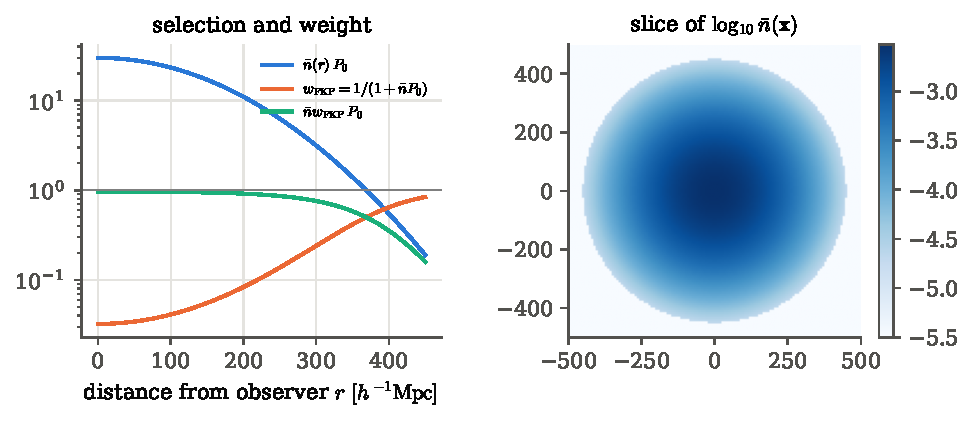
\includegraphics[width=0.92\linewidth]{figures/ch11/fkp_survey.pdf}
\caption{The simulated survey. Left: against distance from the observer, the
signal-to-noise per mode $\bar nP_0$ (blue), the FKP weight (orange) and the
weighted density $\bar nw\,P_0$ (green). Near the observer $\bar nP_0\approx30$
and the weight suppresses the crowded centre; beyond $r\approx370\,h^{-1}$Mpc,
where $\bar nP_0<1$, the weight is close to one. Right: a slice through the box
showing $\log_{10}\bar n$.}
\label{11a:fig:fkp-survey}
\end{figure}

\pyfile[firstline=48,lastline=73,firstnumber=48]{code/ch11/03_fkp.py}{The FKP estimator, its expectation and its predicted variance}

\pyname{fkp_setup} computes, for one weight, the normalisation $I$ (line~49), the
shot noise $P_{\mathrm{shot}}$ with $\alpha\to0$ (line~50), and the exact
expectation \eqref{11a:eq:fkp-mean} (lines~52--54). The last uses the real-space
form of the convolution: the window term is the Fourier transform of $\xi(\bm r)$
times the autocorrelation of $\bar nw$, which is cheaper on a grid than the
convolution itself. Lines~57--60 evaluate the predicted variance
\eqref{11a:eq:fkp-var} for every shell. The main loop (lines~66--73) is
\eqref{11a:eq:fkp-field} and \eqref{11a:eq:fkp-estimator} in four lines; the
random catalogue is replaced by the exact $\bar n$, which is the limit
$\alpha\to0$.

\begin{figure}[htbp]
\centering
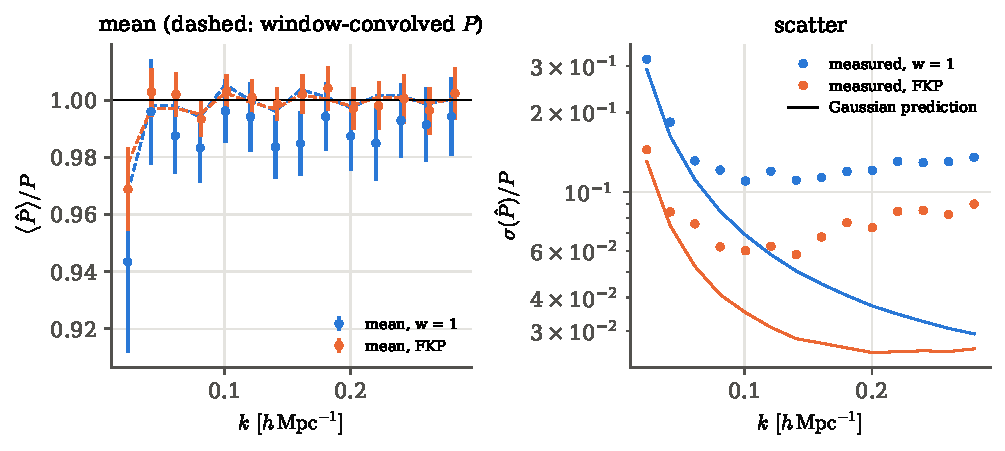
\includegraphics[width=0.95\linewidth]{figures/ch11/fkp_pk.pdf}
\caption{The FKP estimator over $\FkpNsim$ simulated surveys. Left: the mean of
$\hat P$ divided by the true spectrum, for $w=1$ (blue) and the FKP weight
(orange); the dashed curves are the window-convolved expectation
\eqref{11a:eq:fkp-mean}. Right: the scatter of $\hat P/P$ (points) against the
Gaussian prediction \eqref{11a:eq:fkp-var} (lines).}
\label{11a:fig:fkp-pk}
\end{figure}

\Cref{11a:fig:fkp-pk} shows three things. First, the estimator is unbiased once the
window is accounted for: with the FKP weight the mean at
$k=\FkpKb\,h\,\mathrm{Mpc}^{-1}$ is $\FkpMeanB$ times the window-convolved
expectation, and at the lowest $k=\FkpKlow$ the window itself pulls the
expectation down to $\FkpConvLow$ of the true $P$. Second, the FKP weight about
halves the error: the ratio of the FKP scatter to the $w=1$ scatter is
$\FkpRatioA$ at $k=\FkpKa$ and $\FkpRatioB$ at $k=\FkpKb\,h\,\mathrm{Mpc}^{-1}$,
against $\FkpPredA$ and $\FkpPredB$ predicted by \eqref{11a:eq:fkp-var}. The gain
comes despite a shot-noise term that is five times larger with the FKP weight
($P_{\mathrm{shot}}=\FkpShotF$ against $\FkpShotOne\,h^{-3}\mathrm{Mpc}^3$),
because the weight spends shot noise to buy volume. Third, the absolute scatter
is larger than the Gaussian prediction, by a factor $\FkpExcessA$ at
$k=\FkpKa$ and $\FkpExcessB$ at $k=\FkpKb\,h\,\mathrm{Mpc}^{-1}$ for $w=1$. The
Gaussian assumption of \eqref{11a:eq:fkp-var} ignores the four-point function of
the field, and a lognormal field at $z=0$ has a large one on these scales. The
excess affects both weightings alike, so the \emph{ratio} still follows the
Gaussian prediction. For the absolute error, real analyses do not trust
\eqref{11a:eq:fkp-var}; they measure the covariance from mock catalogues
(\cref{11a:sec:research}). For the effective volume of this survey,
\eqref{11a:eq:veff} gives $\FkpVeffKl\,h^{-3}\mathrm{Gpc}^3$ at $k=\FkpKa$ and
$\FkpVeffK$ at $k=\FkpKb\,h\,\mathrm{Mpc}^{-1}$, out of $\FkpVgeo$.
\section{The acoustic peak: a ruler in the galaxy distribution}
\label{11a:sec:bao}

Before the Universe was $400{,}000$ years old, photons and baryons formed a single
fluid, and every overdensity sent out a spherical sound wave through it. When the
baryons were released from the photons, at the drag epoch $z_d\approx1060$, the
waves stopped where they were. Each initial lump of matter is therefore
surrounded by a faint shell of extra baryons at a fixed comoving radius, the
\newterm{sound horizon at the drag epoch}
\begin{equation}
  r_d=\int_{z_d}^{\infty}\frac{c_s(z)\,\dd z}{H(z)},\qquad
  c_s=\frac{c}{\sqrt{3(1+R)}},\quad R=\frac{3\rho_b}{4\rho_\gamma}
  \label{11a:eq:rd}
\end{equation}
\srcref{DESI2024VI}{eqs.~(2.3)--(2.4)}; this is the sound horizon $r_s(\eta)$ of
\cref{T1a:sec:pk} written as an integral over redshift (see the cosmology notes).
For the Planck fiducial model CAMB gives $r_d=\FishRd$\,Mpc. Galaxies form where
matter is dense, so galaxy pairs separated by $r_d$ are slightly more common than
their neighbours: the bump in $\xi(r)$ near $100\,h^{-1}$Mpc that we met in
\cref{T1a:fig:xi} and that \cite{Eisenstein2005} first detected.

What makes the bump valuable is that its length is known. The CMB measures the
physical densities that enter \eqref{11a:eq:rd} so well that $r_d$ is fixed to a
fraction of a percent. A galaxy survey that locates the bump therefore measures
how far away the galaxies are, the way a known ruler seen at an unknown distance
measures the distance through its apparent size. Turning that idea into a
measurement raises three statistical questions. What exactly does a shifted bump tell us? How significant is a bump in a
noisy correlation function? And how precisely can a survey of given size locate
it?

\subsection{What a misplaced bump means: the dilation \texorpdfstring{$\alpha$}{alpha}}
\label{11a:sec:alpha}

\emph{The event.} We turned angles and redshifts into comoving positions using a
fiducial cosmology, computed $\xi(r)$, and found the bump not at
$r_d^{\mathrm{fid}}$, the fiducial model's sound horizon, but a few percent away.

\emph{What could have put it there?} The ruler's true length is $r_d$, which may
differ from the fiducial value. And the distances we used to convert the
catalogue may be wrong. The second effect has two parts, because angles and
redshifts are converted with different distances. Two galaxies at redshift $z$
separated by a small angle $\Delta\theta$ are a transverse distance
$r_\perp=D_M(z)\,\Delta\theta$ apart, where $D_M$ is the comoving angular
diameter distance; two galaxies on the same line of sight separated by $\Delta z$
are a radial distance $r_\parallel=c\,\Delta z/H(z)\equiv D_H(z)\,\Delta z$
apart. (The definitions of $D_M$ and $H(z)$ are in \cref{T1a:sec:objects}.) We
computed both with the fiducial model, so
\begin{align}
  r_\perp^{\mathrm{fid}}
  &\eqby{1}D_M^{\mathrm{fid}}\,\Delta\theta
   \eqby{2}\frac{D_M^{\mathrm{fid}}}{D_M}\,r_\perp
   \equiv\frac{r_\perp}{\alpha_\perp},
  \qquad
  r_\parallel^{\mathrm{fid}}
   \eqby{3}\frac{D_H^{\mathrm{fid}}}{D_H}\,r_\parallel
   \equiv\frac{r_\parallel}{\alpha_\parallel}.
  \label{11a:eq:alpha-perp-par}
\end{align}
\begin{explain}
  \item The observed angle converted with the fiducial distance.
  \item The true separation is $r_\perp=D_M\Delta\theta$, so
        $\Delta\theta=r_\perp/D_M$.
  \item The same for the radial direction, with $D_H=c/H$ in place of $D_M$.
\end{explain}
A true shell of radius $r_d$ therefore appears in the fiducial coordinates with
transverse radius $r_d/\alpha_\perp$ and radial radius $r_d/\alpha_\parallel$.
Measuring both positions relative to the fiducial ruler gives the two numbers that
modern surveys report: $\alpha_\perp=(D_M/r_d)/(D_M/r_d)^{\mathrm{fid}}$ and
$\alpha_\parallel=(D_H/r_d)/(D_H/r_d)^{\mathrm{fid}}$, once the ruler's own
length is included \srcref{DESI2024VI}{\S2.3}. Only the ratios $D_M/r_d$ and
$D_H/r_d$ are measured. A survey cannot tell a longer ruler from a smaller
distance.

\emph{The angle average.} The spherically averaged $\xi(r)$ of a sample with few
galaxies cannot separate the two directions, and sees one overall stretch. A small
volume element is stretched by $\alpha_\perp$ in two directions and
$\alpha_\parallel$ in one, so its volume changes by $\alpha_\perp^2\alpha_\parallel$,
and the isotropic stretch with the same effect on volume is the cube root,
\begin{equation}
  \alpha=\bigl(\alpha_\perp^2\alpha_\parallel\bigr)^{1/3}
  =\frac{D_V/r_d}{(D_V/r_d)^{\mathrm{fid}}},\qquad
  D_V(z)\equiv\bigl[z\,D_M^2(z)\,D_H(z)\bigr]^{1/3}
  \label{11a:eq:dv}
\end{equation}
\srcref{Eisenstein2005}{eq.~(2)}, \srcref{Anderson2012}{eq.~(21)}; the factor $z$
is a convention that gives $D_V$ the units and low-redshift limit of a distance.
Finally, what does a dilation do to the measured correlation function? A pair with
true separation $s$ is placed at $r=s/\alpha$ in the fiducial coordinates, so
\begin{equation}
  \xi_{\mathrm{obs}}(r)=\xi_{\mathrm{true}}(\alpha r),\qquad
  P_{\mathrm{obs}}(k)=\alpha^{-3}P_{\mathrm{true}}(k/\alpha).
  \label{11a:eq:dilation}
\end{equation}
The second form follows from the first by the substitution $\bm s=\alpha\bm r$ in
the Fourier integral; the $\alpha^{-3}$ is the Jacobian.

\begin{keyidea}[The acoustic peak measures a ratio of distances]
A galaxy survey that finds the acoustic peak at a fraction $1/\alpha$ of its
fiducial position measures $D_V(z)/r_d=\alpha\,(D_V/r_d)^{\mathrm{fid}}$ at the
survey's redshift. Splitting the clustering by direction measures $D_M/r_d$ and
$D_H/r_d$ separately. The ruler's length $r_d$ comes from the early Universe; the
distances come from the late Universe; BAO compares the two.
\end{keyidea}

\paragraph{The Alcock--Paczy\'nski idea.}
Even without knowing $r_d$, the \emph{shape} of the clustering carries
information. Structures that are statistically round in the true coordinates look
squashed or stretched along the line of sight if $\alpha_\parallel\ne\alpha_\perp$,
that is, if the fiducial cosmology got the product $D_MH$ wrong. Testing for that
apparent anisotropy is the Alcock--Paczy\'nski test \srcref{DESI2024VI}{\S2.3}.
Its difficulty is that galaxy motions also squash the clustering along the line
of sight (\cref{11a:sec:rsd}), so the two effects must be modelled together;
for the acoustic peak, a sharp feature at a known scale, they separate cleanly.
\Cref{11a:fig:dilation} shows the three cases.

\begin{figure}[htbp]
\centering
\begin{tikzpicture}[scale=0.95]
  \foreach \cx/\ax/\ay/\lab in {0/1.0/1.0/{fiducial = true},4.2/0.87/0.87/{$\alpha_\perp=\alpha_\parallel=1.15$},8.4/1.0/0.80/{$\alpha_\perp=1$, $\alpha_\parallel=1.25$}} {
    \draw[faint,dashed] (\cx,0) circle (1.3);
    \draw[form] (\cx,0) ellipse ({1.3*\ax} and {1.3*\ay});
    \fill[fibreorange] (\cx,0) circle (1.6pt);
    \node[lbl] at (\cx,-1.85) {\lab};
  }
  \draw[->,black!60] (10.3,-1.0) -- (10.3,1.0);
  \node[lbl,anchor=west,align=left] at (10.4,0) {line\\of sight};
\end{tikzpicture}
\caption{The acoustic shell around a galaxy, drawn in the fiducial coordinates.
The dashed circle is where it would appear if the fiducial distances were right.
Middle: true distances $15\%$ larger in every direction make the shell look $15\%$
smaller, an isotropic dilation. Right: a radial distance $25\%$ too small in the
fiducial model, with the transverse one right, squashes the shell along the line
of sight; that anisotropy is the Alcock--Paczy\'nski signal.}
\label{11a:fig:dilation}
\end{figure}

\subsection{A model for the peak, and a fit}
\label{11a:sec:bao-fit}

To locate the bump we fit a template whose bump position is controlled by
$\alpha$. Two physical effects decide what the template looks like.

\emph{The bump is smeared.} Since the drag epoch, galaxies have moved by several
$h^{-1}$Mpc, pushed by large-scale flows. Model each pair separation as shifted by
a Gaussian random displacement with variance $\Sigma_{\mathrm{nl}}^2$ per
component. Then the observed $\xi$ is the true $\xi$ convolved with a Gaussian, and
by the convolution theorem (\cref{7a:sec:convolution}) the power spectrum is
multiplied by the Fourier transform of that Gaussian, $e^{-k^2\Sigma_{\mathrm{nl}}^2/2}$.
Only the oscillating part of $P(k)$ needs this damping, because the smooth part
is handled by the free broad-band terms below. Writing $P_{\mathrm{nw}}$ for a
smooth ``no-wiggle'' spectrum with the same broad shape \cite{EisensteinHu1998},
the template is
\begin{equation}
  P_t(k)=\bigl[P_{\mathrm{lin}}(k)-P_{\mathrm{nw}}(k)\bigr]\,
  e^{-k^2\Sigma_{\mathrm{nl}}^2/2}+P_{\mathrm{nw}}(k)
  \label{11a:eq:template}
\end{equation}
\srcref{Anderson2012}{eq.~(26)}, with $\Sigma_{\mathrm{nl}}=8\,h^{-1}$Mpc for
galaxies as observed and about $4\,h^{-1}$Mpc after ``reconstruction'', a step
that estimates the flows from the galaxy field and moves the galaxies back
\srcref{DESI2024VI}{\S2.3}. Its correlation function $\xi_t(r)$ follows from the
Fourier integral of \cref{T1a:sec:pk}.

\emph{The broad band is uncertain.} Galaxy bias, non-linear growth and the
integral constraint all change the smooth shape of $\xi$ by amounts we do not want
to model. So the fit includes an amplitude and a few smooth nuisance terms:
\begin{equation}
  \xi_{\mathrm{fit}}(r)=B^2\,\xi_t(\alpha r)+a_0+\frac{a_1}{r}+\frac{a_2}{r^2}
  \label{11a:eq:xi-fit}
\end{equation}
\srcref{Anderson2012}{eqs.~(23), (25)}. For a fixed $\alpha$ the model is linear in
$(B^2,a_0,a_1,a_2)$, so for each $\alpha$ on a grid we solve for them by
generalised least squares with the covariance matrix $\Cmat$ of the binned
$\hat\xi$ (\cref{3b:sec:correlated}), and record the minimum
$\chi^2(\alpha)=[\hat{\bm\xi}-\bm\xi_{\mathrm{fit}}]\T\Cmat^{-1}[\hat{\bm\xi}-\bm\xi_{\mathrm{fit}}]$.
This is profiling the nuisance parameters out (\cref{3b:sec:profile}).

\emph{What the fit asks.} The observed event is the measured vector $\hat{\bm\xi}$.
The possible explanations are the values of $\alpha$. For one trial value, the
model predicts a vector $\bm\xi_{\mathrm{fit}}$, and the measurement differs from
that prediction by noise, a Gaussian scatter with covariance $\Cmat$ (the mock
covariance). So for a given $\alpha$ the question is: how plausible is the
particular noise realisation $\hat{\bm\xi}-\bm\xi_{\mathrm{fit}}$ that would turn
the model's prediction into the data we actually have? A Gaussian assigns that
realisation a density proportional to $e^{-\chi^2/2}$, and the same density read
as a function of $\alpha$, with the data held fixed, is the likelihood
(\cref{ch:03}). The best $\alpha$ is where the required noise is least
surprising, that is, where $\chi^2(\alpha)$ is smallest. With a flat prior in
$\alpha$ the posterior is $p(\alpha)\propto e^{-\chi^2(\alpha)/2}$, and its width
is the uncertainty \srcref{Anderson2012}{eqs.~(27)--(29)}.

\subsection{How significant is a bump? \texorpdfstring{$\Delta\chi^2$}{Delta chi2} and the number of sigma}
\label{11a:sec:bao-signif}

Eisenstein and collaborators quoted their detection as ``$3.4\sigma$'', from the
difference in $\chi^2$ between the best model without the acoustic feature and the
best model with it, $\Delta\chi^2=11.7$ \srcref{Eisenstein2005}{\S4.3}. Before
reproducing the number we should see why $\sqrt{\Delta\chi^2}$ is a number of
sigma.

Give the bump an amplitude $A$: the model is the smooth part plus $A$ times the
difference between the templates with and without the feature, so $A=1$ is the
full acoustic signal and $A=0$ is none. The model is linear in $A$, and with
Gaussian errors $\chi^2$ is then exactly quadratic in $A$ (\cref{3b:sec:chi2-min}):
$\chi^2(A)=\chi^2_{\min}+(A-\hat A)^2/\sigma_A^2$, where $\hat A$ is the best fit
and $\sigma_A$ its standard error. Then
\begin{align}
  \Delta\chi^2\equiv\chi^2(0)-\chi^2(1)
  &\eqby{1}\frac{\hat A^2-(1-\hat A)^2}{\sigma_A^2}
   \eqby{2}\frac{2\hat A-1}{\sigma_A^2},
  \qquad\text{and if }\hat A=1:\quad
  \sqrt{\Delta\chi^2}\eqby{3}\frac{\hat A}{\sigma_A}.
  \label{11a:eq:dchi2-sigma}
\end{align}
\begin{explain}
  \item Insert $A=0$ and $A=1$ into the quadratic; $\chi^2_{\min}$ cancels.
  \item $\hat A^2-(1-2\hat A+\hat A^2)=2\hat A-1$.
  \item With $\hat A=1$, $\Delta\chi^2=1/\sigma_A^2=(\hat A/\sigma_A)^2$.
\end{explain}
So when the data prefer the full acoustic amplitude, $\sqrt{\Delta\chi^2}$ is the
number of standard errors by which the bump's amplitude differs from zero: a
signal-to-noise ratio.

The same number can be read as a test. Let $A$ float and take as the null
hypothesis ``there is no acoustic bump'', $A=0$. It is the hypothesis whose sampling distribution we know:
if it were true, $\chi^2(0)-\chi^2(\hat A)$ would follow a $\chi^2$ distribution
with one degree of freedom (Wilks' theorem, \cref{4a:sec:wilks}). The question
for the data is then: if there were no bump, would a $\Delta\chi^2$ as large as
$11.7$, or larger, be something we would reasonably expect from noise alone? The
tail probability of a $\chi^2_1$ beyond $11.7$ is $6\times10^{-4}$, which is the
two-sided Gaussian probability of lying more than $\sqrt{11.7}=3.4$ standard
deviations out (\cref{4a:sec:p-to-z}). So noise alone would produce a bump this
strong about once in sixteen hundred surveys.
Both readings give the same rule of thumb: for one extra parameter, the square
root of the drop in $\chi^2$ counts the sigmas.

\subsection{Reproducing the first detection on mock surveys}
\label{11a:sec:bao-mocks}

\emph{What the paper compared.} Eisenstein and collaborators measured $\xi(s)$ in
redshift space, spherically averaged, with the Landy--Szalay estimator
(\cref{11a:sec:xi}) and FKP-like weights with $P_w=4\times10^4$, in 20 bins out to
$180\,h^{-1}$Mpc. The covariance came from $1278$ mock catalogues. They fitted
models of $\xi$ with a free amplitude and free $\Omega_mh^2$ and a dilation of the
scale, \eqref{11a:eq:dilation}. The best model with baryons had $\chi^2=16.1$ for
17 degrees of freedom; the best pure cold-dark-matter model, which has no acoustic
feature, had $\chi^2=27.8$, so $\Delta\chi^2=11.7$, ``$3.4\sigma$'' by
\eqref{11a:eq:dchi2-sigma} \srcref{Eisenstein2005}{\S3.1, \S4.3, Fig.~6}. The
quantity to reproduce is $\Delta\chi^2$: how strongly a survey of that size
prefers a template with the peak over one without it.

\emph{Our nerfed version.} The script \pyname{code/ch11/04_bao_mocks.py} replaces
the survey by a periodic box of the same volume, side $\BaoL\,h^{-1}$Mpc
($\BaoVol\,h^{-3}\mathrm{Gpc}^3$), holding the same number of galaxies,
$\bar n=\BaoNbar\times10^{-5}\,h^3\mathrm{Mpc}^{-3}$ (about $\BaoNgal$ per box).
The galaxy field is lognormal with spectrum $b^2D^2(z)\,K_0\,P_t(k)$, with
$z=\BaoZ$, $b=\BaoB$, growth factor $D=\BaoD$, damping
$\Sigma_{\mathrm{nl}}=\BaoSigNl\,h^{-1}$Mpc, and $K_0=\BaoKaiserZero$ the
angle-averaged boost of the clustering amplitude by galaxy motions
(\cref{11a:sec:rsd}). Its amplitude, $\sigma_{8,g}=\BaoSigEightG$, is close to the
value $1.8$ that the paper assumed for the LRGs. In the box there are no edges, so
$\xi$ is estimated by Fourier-transform pair counting on the grid ($\BaoN^3$
cells), which is what all four estimators of \cref{11a:sec:xi} reduce to without
edges. We use $\BaoNbins$ bins of $10\,h^{-1}$Mpc from $20$ to $180\,h^{-1}$Mpc.
$\BaoNcov$ mocks give the covariance, with the Hartlap factor $\BaoHartlap$
(\cref{8b:sec:hartlap}); $\BaoNfit$ further mocks are each fitted with
\eqref{11a:eq:xi-fit}, once with the template \eqref{11a:eq:template} and once
with the no-wiggle template, on a grid of $\alpha\in[0.8,1.2]$.

\pyfile[firstline=54,lastline=95,firstnumber=54]{code/ch11/04_bao_mocks.py}{Templates, mocks and the fit}

\pyname{template_bins} builds the model for any $\alpha$ through the Fourier form of
\eqref{11a:eq:dilation}: the spectrum $P(k/\alpha)/\alpha^3$ is turned into the
grid correlation function and averaged in the same bins as the data, so that the
model and the measurement see exactly the same grid. The mock loop (lines
67--72) is \cref{11a:sec:cox} in four lines: lognormal field, Poisson galaxies,
density contrast with the box's own mean (so the integral constraint is present),
pair counting by FFT. Lines~76--79 form the covariance and its Hartlap-corrected
inverse. In \pyname{fit}, line~93 is the generalised least-squares solution
$(X\T\Cmat^{-1}X)^{-1}X\T\Cmat^{-1}\hat{\bm\xi}$ for the four linear coefficients
at each $\alpha$.

\begin{figure}[htbp]
\centering
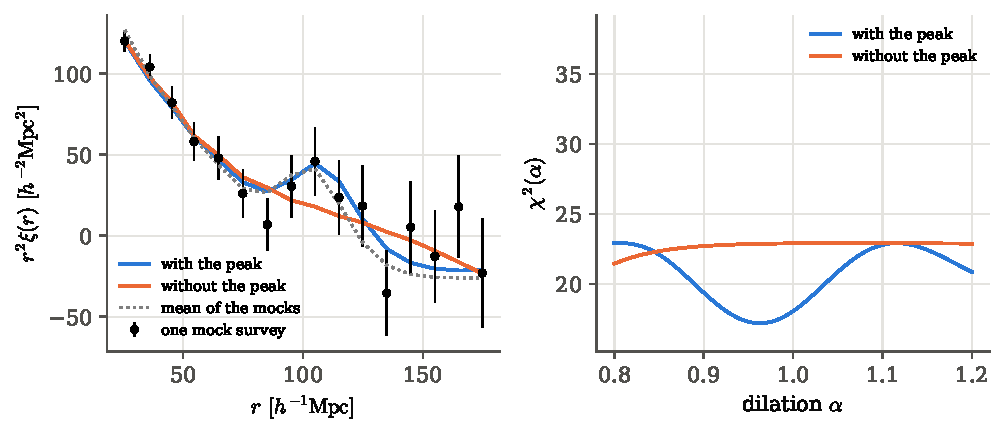
\includegraphics[width=0.95\linewidth]{figures/ch11/bao_mock_fit.pdf}
\caption{One mock survey, chosen as the one with the median $\Delta\chi^2$ among
the $\BaoNfit$ fitted. Left: $r^2\hat\xi(r)$ (points, with the diagonal errors of
the mock covariance; neighbouring points are correlated), the mean over mocks
(dotted) and the best fits with and without the acoustic feature. Right:
$\chi^2(\alpha)$ for both templates. The template with the peak has a minimum
near $\alpha=1$; the one without is almost flat, because nothing in it marks a
scale.}
\label{11a:fig:bao-fit}
\end{figure}

\Cref{11a:fig:bao-fit} shows a typical mock. Its best fit with the peak has
$\chi^2=\BaoExChiW$ for $\BaoDof$ degrees of freedom and $\hat\alpha=\BaoExAlpha$;
the no-wiggle template is worse by $\Delta\chi^2=\BaoExDchi$. Over all fitted
mocks the mean $\chi^2$ of the peak template is $\BaoMeanChiW$, close to the
$\BaoDof$ expected if the covariance is right, and the mean $\hat\alpha$ is
$\BaoMeanAlpha\pm\BaoErrMeanAlpha$: the fit is unbiased.

\begin{figure}[htbp]
\centering
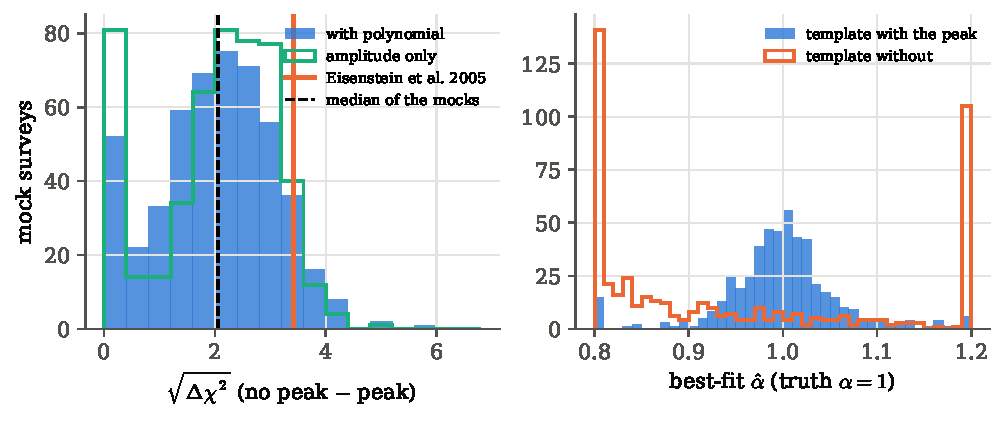
\includegraphics[width=0.95\linewidth]{figures/ch11/bao_mock_detect.pdf}
\caption{Left: the detection significance $\sqrt{\Delta\chi^2}$ over $\BaoNfit$ mock
surveys of the size of the SDSS LRG sample, with the broad-band polynomial
(filled) and with the amplitude as the only free coefficient (green outline). The
dashed line is the median, the orange line the $3.4\sigma$ of the 2005 paper.
Right: the best-fit dilation with the peak template (filled) and with the
no-wiggle template (outline), which wanders to the edges of the allowed range.}
\label{11a:fig:bao-detect}
\end{figure}

\Cref{11a:fig:bao-detect} is the reproduction. A survey of that volume and density
typically detects the acoustic peak at $\sqrt{\Delta\chi^2}=\BaoMedSig$ (the
middle $68\%$ of mocks lie between $\BaoSigLo$ and $\BaoSigHi$), and
$\BaoFracEis\%$ of mock surveys reach the paper's $\Delta\chi^2=11.7$. Fitting as the
paper did, with the amplitude as the only free coefficient, changes little: median
$\BaoMedSigE$, and $\BaoFracEisE\%$ reach $3.4\sigma$. So the qualitative
result reproduces: a survey of $0.7\,h^{-3}\mathrm{Gpc}^3$ at $\bar nP\sim1$ does
see the peak, at a modest significance. The 2005 detection sits in the upper
tail. Part of that is the luck of one realisation, which the paper's own Figure~2
hints at (the measured points sit above every model). Part is that their
comparison model, cold dark matter without baryons, differs from the baryonic
model in its broad shape as well as in the peak, and their fit reached down to
$10\,h^{-1}$Mpc, where that shape difference adds to $\Delta\chi^2$; our no-wiggle
template differs from the peak template \emph{only} in the peak.

The dilation is measured to $\BaoSdAlpha\%$ (standard deviation of $\hat\alpha$ over
mocks; the median per-mock error from $p(\alpha)$ is $\BaoMedSigAlpha\%$),
against the paper's $4.7\%$ on $D_V(0.35)$, which also includes the shape
information. Without the peak, the dilation is barely constrained
($\BaoSdAlphaNw\%$, limited by the edges of the grid). The paper found the same
contrast: its pure-CDM fit constrained the scale a factor of two worse
\srcref{Eisenstein2005}{\S4.3}. The distance information is in the peak.

\subsection{How well can a survey locate the peak? A Fisher forecast}
\label{11a:sec:bao-fisher}

The mocks answer the question for one survey at the cost of two thousand
simulations. The Fisher matrix of \cref{ch:10} answers it for any survey in a
fraction of a second. The data are the Fourier modes $\delta_{\bm k}$ of the galaxy
field; the parameter is $\alpha$. For a Gaussian mode whose variance depends on the
parameter, the Fisher information is
$F=\frac12\tr[\Cmat^{-1}\Cmat_{,\alpha}\Cmat^{-1}\Cmat_{,\alpha}]$
(\cref{10a:sec:gauss}; \srcref{HobsonBMC}{\S5.3.1, eq.~(5.17)}). A complex mode
$\delta_{\bm k}$ is two real Gaussian numbers, its real and imaginary parts, each
with variance $\frac V2[P(k)+1/\bar n]$ in a box of volume $V$ with uniform
density (\cref{7a:sec:grf-fourier}). Modes at $\bm k$ and $-\bm k$ are the same
mode, so a shell of width $\dd k$ holds $\frac12\,V\,4\pi k^2\dd k/(2\pi)^3$
independent complex modes. Then
\begin{align}
  F_{\alpha\alpha}
  &\eqby{1}\sum_{\text{modes}}2\times\frac12
     \Bigl(\frac{\partial_\alpha P}{P+1/\bar n}\Bigr)^2
   \eqby{2}\int\frac{V\,4\pi k^2\,\dd k}{2(2\pi)^3}
     \Bigl(\frac{\bar nP}{1+\bar nP}\Bigr)^2
     \Bigl(\frac{\partial\ln P}{\partial\alpha}\Bigr)^2\nonumber\\
  &\eqby{3}\int\frac{k^2\,\dd k}{4\pi^2}\;V_{\mathrm{eff}}(k)\,
     \Bigl(\frac{\partial\ln P}{\partial\alpha}\Bigr)^2 .
  \label{11a:eq:fisher-alpha}
\end{align}
\begin{explain}
  \item For one real Gaussian variable of variance $v(\alpha)$,
        $\frac12(v_{,\alpha}/v)^2$; each complex mode contributes two such
        variables, and the shot noise does not depend on $\alpha$.
  \item Replace the sum by the mode count of the shell, and write
        $\partial_\alpha P/(P+1/\bar n)=\frac{\bar nP}{1+\bar nP}\,\partial_\alpha\ln P$.
  \item $4\pi/(2(2\pi)^3)=1/(4\pi^2)$, and
        $V[\bar nP/(1+\bar nP)]^2=V_{\mathrm{eff}}(k)$, which for a survey with
        varying $\bar n$ becomes the integral \eqref{11a:eq:veff}.
\end{explain}
This is the forecast formula of Seo and Eisenstein \srcref{SeoEisenstein2003}{eq.~(9)},
and it is the same effective volume that measured the error of $\hat P$ in
\cref{11a:sec:fkp}. The derivative must contain only the information in the peak,
since the broad band is marginalised in the fit. With
$P(k;\alpha)=P_{\mathrm{nw}}(k)\,[1+O(k/\alpha)]$, where
$O=(P_t-P_{\mathrm{nw}})/P_{\mathrm{nw}}$ is the damped wiggle pattern,
\begin{equation}
  \frac{\partial\ln P}{\partial\alpha}\Big|_{\alpha=1}=-\frac{k\,O'(k)}{1+O(k)} .
  \label{11a:eq:dlnp-dalpha}
\end{equation}
The error forecast is $\sigma_\alpha=F_{\alpha\alpha}^{-1/2}$.

\pyfile[firstline=33,lastline=44,firstnumber=33]{code/ch11/05_bao_fisher.py}{The Fisher error on $\alpha$}

\begin{figure}[htbp]
\centering
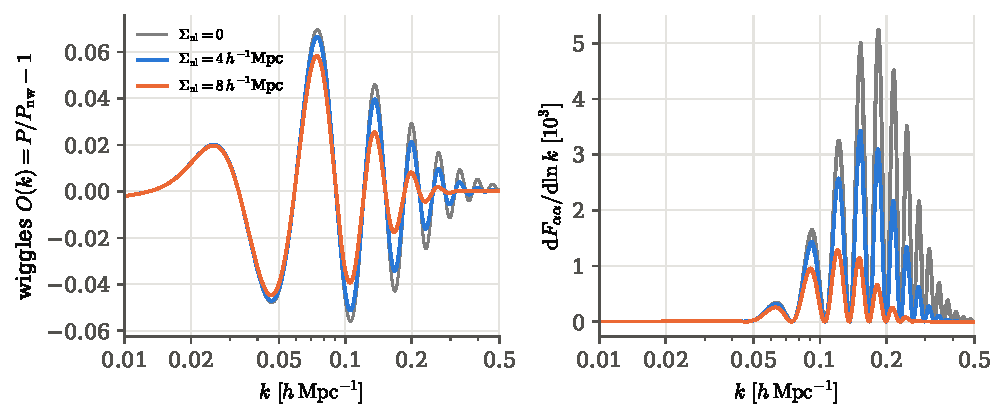
\includegraphics[width=0.95\linewidth]{figures/ch11/bao_fisher.pdf}
\caption{Where the information on $\alpha$ comes from. Left: the wiggle pattern
$O(k)$ undamped (grey) and damped with $\Sigma_{\mathrm{nl}}=4$ (blue) and $8\,h^{-1}$Mpc
(orange). Right: the Fisher integrand of \eqref{11a:eq:fisher-alpha} per $\ln k$ for
the mock box, with the same colours. The information sits in the wiggles between
$k\approx0.05$ and $0.3\,h\,\mathrm{Mpc}^{-1}$; damping erases the higher harmonics.}
\label{11a:fig:bao-fisher}
\end{figure}

\paragraph{Example: the mock box.}
For the box of \cref{11a:sec:bao-mocks}, \eqref{11a:eq:fisher-alpha} predicts
$\sigma_\alpha=\FishBox\%$. The mocks gave $\FishMockSd\%$ (scatter of $\hat\alpha$)
and $\FishMockMed\%$ (median per-mock error). The forecast is optimistic, and it is
supposed to be: the inverse Fisher matrix is a lower bound (\cref{10a:sec:cr}),
reached only when the likelihood for $\alpha$ is close to Gaussian. At a typical
detection of $2\sigma$ it is not: $\chi^2(\alpha)$ in \cref{11a:fig:bao-fit} is
shallow, with secondary minima where a noise fluctuation mimics the peak, and in
some mocks the fit wanders to the edge of the grid. The bound becomes accurate
only for high signal-to-noise. The lognormal field's non-Gaussian covariance,
seen already in \cref{11a:sec:fkp-python}, adds to the gap.

\paragraph{Example: the 2005 survey.}
For the survey rebuilt from the paper's numbers in \cref{11a:sec:fkp} (with
$\bar n(z)$, the paper's galaxy amplitude $\sigma_{8,g}=1.8$, and
$\Sigma_{\mathrm{nl}}=8\,h^{-1}$Mpc), the forecast is $\sigma_\alpha=\FishEis\%$.
The paper reports $D_V(0.35)=1370\pm64$\,Mpc, a $4.7\%$ distance. Compared with
the distance to the last-scattering surface it is the ratio
$R_{0.35}=D_V(0.35)/D_M(1089)=0.0979\pm0.0036$, a $3.7\%$ measurement. And the
dimensionless combination $A=D_V(0.35)\sqrt{\Omega_mH_0^2}/(0.35\,c)=0.469\pm0.017$
($3.6\%$) is the distance measured in units of $c/(\sqrt{\Omega_m}H_0)$, a combination
that depends on the other parameters only weakly \srcref{Eisenstein2005}{Table~1}.

\paragraph{Example: DESI's bright galaxies.}
DESI's first data release measured, from 300,017 bright galaxies at
$0.1<z<0.4$, $D_V/r_d=7.93\pm0.15$ at $z_{\mathrm{eff}}=0.295$, a $\FishDesiFrac\%$
measurement, after reconstruction, with a quoted effective volume of
$1.7\,\mathrm{Gpc}^3$ \srcref{DESI2024VI}{Table~1}. In our units that is
$\FishDesiVh\,h^{-3}\mathrm{Gpc}^3$. Taking that $V_{\mathrm{eff}}$ as if it held at
every $k$, \eqref{11a:eq:fisher-alpha} forecasts $\FishDesiRec\%$ with the
post-reconstruction damping $\Sigma_{\mathrm{nl}}=4\,h^{-1}$Mpc and $\FishDesiPre\%$
with the pre-reconstruction $8\,h^{-1}$Mpc. The measured error lies between the two.
The simple forecast is optimistic for the same reasons as before, plus one: a
single $V_{\mathrm{eff}}$ quoted at one reference wavenumber overstates the
information at higher $k$, where $\bar nP$ is smaller.

\begin{inpractice}
Our mock boxes play the role of a \emph{verification}: the Fisher formula
\eqref{11a:eq:fisher-alpha} is a known answer for Gaussian modes, and the mocks
check it and show where it fails (low signal-to-noise, non-Gaussian covariance).
In a survey analysis the same machinery becomes the \emph{research instrument}.
For a real footprint, with its mask, its varying $\bar n$, fibre collisions and
reconstruction, there is no formula for the covariance of $\hat\xi$ or for the
scatter of $\hat\alpha$; the only way to obtain them is to push a thousand or so
mock catalogues through the full pipeline, or to calibrate a semi-analytic
covariance against them (\cref{11a:sec:research}).
\end{inpractice}

\subsection{Comparing with the data: DESI distances against Planck}
\label{11a:sec:bao-desi}

\Cref{11a:fig:bao-desi} puts the DESI DR1 distances next to the prediction of the
Planck 2018 $\Lambda$CDM model. For the anisotropic measurements we form
$D_V/r_d=(z\,(D_M/r_d)^2\,(D_H/r_d))^{1/3}$ from the published $D_M/r_d$ and
$D_H/r_d$, with the error from the delta method (\cref{3a:sec:delta}): for
$\ln D_V=\frac13(2\ln D_M+\ln D_H+\ln z)$,
\begin{equation}
  \frac{\sigma_{D_V}}{D_V}=\frac13\sqrt{4\Bigl(\frac{\sigma_{D_M}}{D_M}\Bigr)^2
  +\Bigl(\frac{\sigma_{D_H}}{D_H}\Bigr)^2
  +4\rho\,\frac{\sigma_{D_M}}{D_M}\frac{\sigma_{D_H}}{D_H}},
  \label{11a:eq:dv-error}
\end{equation}
where $\rho$ is the published correlation coefficient between the two.

\begin{figure}[htbp]
\centering
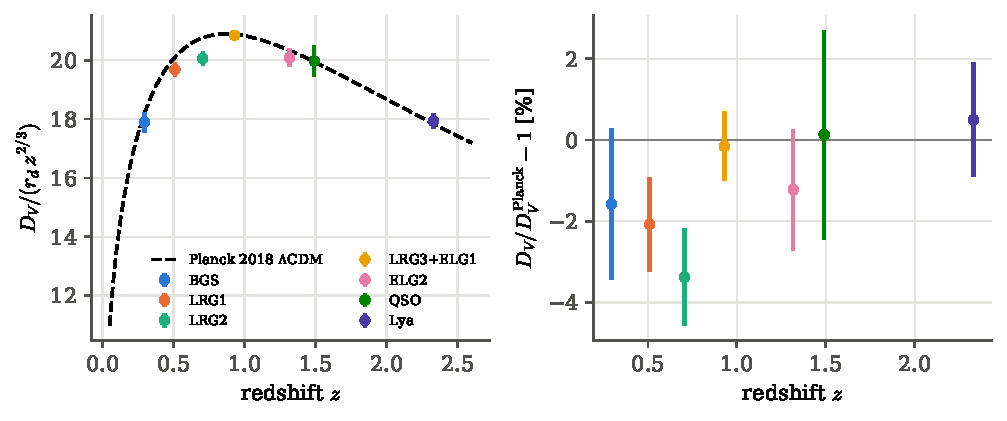
\includegraphics[width=0.95\linewidth]{figures/ch11/bao_desi.pdf}
\caption{DESI DR1 BAO distances (points; \cite{DESI2024VI}, Table~1) against the
Planck 2018 $\Lambda$CDM prediction (dashed). Left: $D_V/r_d$, divided by $z^{2/3}$ to
flatten the curve. Right: the fractional difference from the prediction.}
\label{11a:fig:bao-desi}
\end{figure}

The bright-galaxy point, $7.93\pm0.15$, sits $\FishBgsPull\sigma$ from the
Planck prediction $\FishBgsPred$. The largest deviation is the luminous red galaxy
bin at $z=0.71$, $\FishLrgTwoDv\pm\FishLrgTwoSd$ against $\FishLrgTwoPred$, a
$\FishMaxPull\sigma$ pull. Taken together, the $\FishNpts$ points give
$\chi^2=\FishChiTwo$ for $\FishNpts$ degrees of freedom, a $p$-value of
$\FishChiP$. How surprised should we be by one $\FishMaxPull\sigma$ point? Among
$\FishNpts$ independent points, the chance that at least one deviates by that
much is $\FishMaxP$, which is the look-elsewhere correction of
\cref{4b:sec:lee}. The data are compatible with the Planck model at the level of
this simple comparison; the cosmological fits in the DESI paper, which use the two
directions separately and add other data, are where the interesting tensions are
argued.

\emph{Where we have met $H_0$ before.} These are the same twelve DESI numbers that \cref{T2b:sec:bao} fitted on a grid
in $(\Omega_m,hr_d)$, finding $hr_d=101.8\pm1.3$\,Mpc; with the sound horizon $r_d=147.09$\,Mpc taken from the CMB,
that became an inverse distance ladder, $H_0=69.2\pm0.9$, near Planck's $67.36\pm0.54$ and well below the
$73.04\pm1.04$ of the supernova ladder (\cref{T2b:sec:tension}). The degeneracy is the same here: every $D/r_d$
depends on $H_0$ and $r_d$ only through their product, as the supernova magnitudes of \cref{3b:sec:hubble-degeneracy}
depended on $H_0$ and $M$ only through $M-5\log_{10}H_0$. What differs is that nothing is fitted. Planck's model,
with its $H_0=67.36$ and $r_d=\FishRd$\,Mpc, is held fixed, so the comparison tests their product, $hr_d=99.1$\,Mpc,
and the shape of the distance curve, never $H_0$ on its own; and each bin is reduced to the single number $D_V/r_d$.
The verdicts differ for that reason: there, $\Delta\chi^2=8.3$ between the Planck point and the best fit, with two
degrees of freedom, gave $p=0.016$; here the absolute $\chi^2$ spreads the same disagreement over $\FishNpts$ degrees of
freedom and gives $p=\FishChiP$. \Cref{11c:sec:h0-routes} sets this route beside the other routes to $H_0$.
\section{Galaxy motions: clustering in redshift space}
\label{11a:sec:rsd}

A survey never measures how far away a galaxy is. It measures a redshift, and
turns it into a distance with the Hubble law of a fiducial cosmology. The
redshift, though, is not only the stretching of light by the expansion. Every
galaxy also moves through space with its own \newterm{peculiar velocity}, a few
hundred kilometres per second, and the part of that velocity along our line of
sight adds a Doppler shift. The survey therefore places each galaxy a little in
front of or a little behind its true position, and only along the line of sight.

If these velocities were random, the displacement would be a nuisance that blurs
the map. They are not random. Galaxies fall towards overdense regions and stream
out of empty ones, pulled by the same gravity that makes the overdensities grow.
On large scales a galaxy in front of a supercluster falls away from us, towards
the supercluster, and is placed further away; a galaxy behind it falls towards
us and is placed nearer. Both move towards the centre in the map. The
supercluster looks squashed along the line of sight and denser than it is. The
size of the squashing is set by how fast the infall is, and that is set by how
fast structure grows. A direction-dependent clustering pattern thus becomes a
measurement of the growth rate of structure, the second number, after the
acoustic scale of \cref{11a:sec:bao}, that a galaxy survey hands to cosmology.

The question, in words:
\begin{quote}
\emph{If every galaxy is moved along the line of sight by its own velocity, and
the velocities are the ones that gravity produces while structure is still
small, how does the power spectrum of the moved galaxies depend on the angle
between a Fourier mode and the line of sight?}
\end{quote}

\subsection{From a redshift to a misplaced galaxy}
\label{11a:sec:rsd-map}

\emph{The event.} A galaxy is observed at redshift $z_{\mathrm{obs}}$, and we put it
at the comoving distance $\chi(z_{\mathrm{obs}})$.

\emph{What produced that redshift?} Two shifts, one after the other. Think of a
comoving observer \unpack{one at rest with respect to the expansion} sitting
right next to the galaxy. The galaxy moves away from this neighbour with
line-of-sight velocity $u_r$, so the neighbour sees light of emitted frequency
$\nu_e$ at $\nu'=\nu_e/(1+u_r/c)$, the ordinary non-relativistic Doppler shift
($u_r\sim300$\,km\,s$^{-1}$ is a thousandth of $c$). That light then travels to
us through the expanding Universe and is stretched by the cosmological factor
$1+z_c$, where $z_c$ is the redshift the galaxy would have if it were at rest:
$\nu_0=\nu'/(1+z_c)$. Frequency ratios multiply, so
\begin{equation}
  1+z_{\mathrm{obs}}=\frac{\nu_e}{\nu_0}=(1+z_c)\Bigl(1+\frac{u_r}{c}\Bigr).
  \label{11a:eq:z-compose}
\end{equation}
(Our own motion adds a third factor of the same kind; it is the same for every
galaxy in a given direction and is removed by quoting redshifts in the rest frame
of the CMB.) The peculiar velocity is $\bm u=a\,\dot{\bm x}$, the rate of change
of comoving position $\bm x$ times the scale factor $a$, which is how the
cosmology notes define it; $u_r=\bm u\cdot\hat{\bm r}$ is its component along the
line of sight $\hat{\bm r}$.

\emph{Where does the galaxy land?} We convert $z_{\mathrm{obs}}$ with the comoving
distance $\chi(z)=\int_0^z c\,\dd z'/H(z')$. Calling the assigned distance $s$,
\begin{align}
  s\equiv\chi(z_{\mathrm{obs}})
  &\eqby{1}\chi(z_c)+\frac{\dd\chi}{\dd z}\Big|_{z_c}\,(z_{\mathrm{obs}}-z_c)
  \eqby{2}\chi+\frac{c}{H(z)}\,(1+z)\,\frac{u_r}{c}
  \eqby{3}\chi+\frac{u_r}{aH}.
  \label{11a:eq:rsd-map}
\end{align}
\begin{explain}
  \item A first-order Taylor expansion; the shift $z_{\mathrm{obs}}-z_c$ is of
        order $10^{-3}(1+z)$, so the next term is a million times smaller than
        $\chi$.
  \item $\dd\chi/\dd z=c/H(z)$ from the integral, and
        $z_{\mathrm{obs}}-z_c=(1+z_c)\,u_r/c$ from \eqref{11a:eq:z-compose}. We
        drop the subscript on $z_c$ in factors that multiply a small quantity.
  \item $1+z=1/a$.
\end{explain}
The true comoving distance is $\chi$; the galaxy is placed at $s$, displaced by
$u_r/(aH)$ along the line of sight. In vector form,
$\bm s=\bm x+\bigl(u_r/aH\bigr)\,\hat{\bm r}$. The space of the assigned positions
$\bm s$ is called \newterm{redshift space}; the space of the true positions
$\bm x$ is \newterm{real space}.

\paragraph{Example: how far is a galaxy moved?}
Near us, $a=1$ and $H=H_0=100\,h$\,km\,s$^{-1}$Mpc$^{-1}$. A galaxy falling at
$300$\,km\,s$^{-1}$ is moved by $300/100=3\,h^{-1}$Mpc. A galaxy orbiting inside a
rich cluster at $1000$\,km\,s$^{-1}$ is moved by $10\,h^{-1}$Mpc. The first number
is small against the $100\,h^{-1}$Mpc acoustic scale, but not against the
$10$--$30\,h^{-1}$Mpc separations where most pairs sit; the second is larger
than the cluster itself.

For the rest of the section we look at a patch of the survey far from us and
small on the sky, so that every line of sight in it points in nearly the same
direction. Call that direction $\hat{\bm z}$. This is the
\newterm{distant-observer approximation}. The mapping is then a shift along one
fixed axis,
\begin{equation}
  \bm s=\bm x+v_z(\bm x)\,\hat{\bm z},\qquad v_z\equiv\frac{u_z}{aH},
  \label{11a:eq:rsd-map-pp}
\end{equation}
where $v_z$ is the line-of-sight velocity expressed as a comoving distance. For a
Fourier mode with wavevector $\bm k$, let $\mu=\hat{\bm k}\cdot\hat{\bm z}$ be the
cosine of its angle with the line of sight: $\mu=\pm1$ for a wave whose crests
are perpendicular to the line of sight, $\mu=0$ for crests along it.

\subsection{Counting galaxies twice: the Kaiser factor}
\label{11a:sec:kaiser}

We want the density contrast of the galaxies in redshift space,
$\delta_s(\bm s)$, in terms of the real-space field. We state the inputs first,
as in \cref{11a:sec:cox-inputs}.

\emph{Physical inputs:}
\begin{enumerate}[label=(K\arabic*),leftmargin=2.6em,itemsep=1pt]
  \item \emph{Galaxies are conserved by the mapping.} Each galaxy appears exactly
        once in the redshift-space catalogue. This is bookkeeping, and exact.
  \item \emph{Linear theory.} The density contrast and the velocities are small,
        and the matter velocity field obeys the linear continuity equation of the
        cosmology notes,
        \begin{equation}
          \theta\equiv\frac{\nabla\cdot\bm u}{aH}=-f\,\delta,\qquad
          f\equiv\frac{\dd\ln D}{\dd\ln a},
          \label{11a:eq:theta}
        \end{equation}
        with $\delta$ the matter contrast, $D(a)$ the linear growth factor
        \unpack{how much a small fluctuation has grown by scale factor $a$} and
        $f$ the \newterm{growth rate}. The velocity field has no curl (linear
        rotational modes decay; see the cosmology notes).
  \item \emph{Galaxies trace the matter.} Their density contrast is
        $\delta_g=b\,\delta$ with a constant linear bias $b$, and they move with
        the matter, because gravity accelerates a galaxy and the dark matter
        around it in the same way.
\end{enumerate}
\emph{Geometric input:} the distant-observer approximation of
\eqref{11a:eq:rsd-map-pp}. \emph{Mathematical input:} the mapping
$\bm x\mapsto\bm s$ is smooth and one-to-one, which holds while $v_z$ changes
by much less than the distance over which it changes, that is while
$\abs{\partial_zv_z}\ll1$. (In a collapsing cluster it fails: two galaxies at
different true positions can land at the same $\bm s$.)

\emph{The galaxies in a small volume, counted twice.} The galaxies inside a small
real-space volume $\dd^3x$ around $\bm x$ end up inside a redshift-space volume
$\dd^3s$ around $\bm s$, and by (K1) they are the same galaxies. With $\bar n$ the
mean density (the same in both spaces, since the shifts average to zero),
$\bar n[1+\delta_s(\bm s)]\,\dd^3s=\bar n[1+\delta_g(\bm x)]\,\dd^3x$. The ratio of
the volumes is the Jacobian of the mapping \eqref{11a:eq:rsd-map-pp}. Its matrix
$\partial s_i/\partial x_j$ has rows $(1,0,0)$, $(0,1,0)$ and
$(\partial_xv_z,\partial_yv_z,1+\partial_zv_z)$; it is triangular, so its
determinant is the product of the diagonal entries, $1+\partial_zv_z$. Hence
\begin{align}
  1+\delta_s(\bm s)
  &\eqby{1}\frac{1+\delta_g(\bm x)}{1+\partial_zv_z(\bm x)}
   \eqby{2}1+\delta_g(\bm x)-\partial_zv_z(\bm x)+O(\delta^2),
  \nonumber\\
  \delta_s(\bm x)
  &\eqby{3}\delta_g(\bm x)-\partial_zv_z(\bm x)+O(\delta^2).
  \label{11a:eq:rsd-jacobian}
\end{align}
\begin{explain}
  \item Number conservation, divided by $\bar n\,\dd^3s$, with
        $\dd^3x/\dd^3s=1/(1+\partial_zv_z)$.
  \item $1/(1+\epsilon)=1-\epsilon+\epsilon^2-\dots$, and the product
        $\delta_g\,\partial_zv_z$ is second order, so it is dropped with the rest.
  \item $\delta_s(\bm s)=\delta_s(\bm x+v_z\hat{\bm z})
        =\delta_s(\bm x)+v_z\,\partial_z\delta_s+\dots$; the correction is again a
        product of two small quantities.
\end{explain}
So in linear theory the redshift-space contrast is the real-space contrast minus
the line-of-sight gradient of the line-of-sight velocity. Where galaxies on the
near side move away from us and those on the far side move towards us,
$\partial_zv_z<0$: the galaxies crowd together in the map and $\delta_s$ grows.

\emph{The velocity in terms of the density.} Now use (K2). Since the velocity
field has no curl it is a gradient, $\bm u/(aH)=\nabla\phi$ for some potential
$\phi$. In Fourier space a gradient is multiplication by $i\bm k$. Then
\begin{align}
  -k^2\phi_{\bm k}
  &\eqby{1}i\bm k\cdot\bigl(i\bm k\,\phi_{\bm k}\bigr)
   \eqby{2}\theta_{\bm k}
   \eqby{3}-f\,\delta_{\bm k},
  \qquad\text{so}\qquad
  \Bigl(\frac{\bm u}{aH}\Bigr)_{\bm k}=i\bm k\,\phi_{\bm k}
   =\frac{i\bm k}{k^2}\,f\,\delta_{\bm k},
  \nonumber\\
  \bigl(\partial_zv_z\bigr)_{\bm k}
  &\eqby{4}(ik_z)\,\frac{ik_z}{k^2}\,f\,\delta_{\bm k}
   \eqby{5}-f\mu^2\,\delta_{\bm k}.
  \label{11a:eq:dvdz}
\end{align}
\begin{explain}
  \item $\bm k\cdot\bm k=k^2$ and $i^2=-1$.
  \item The divergence of $\bm u/(aH)=\nabla\phi$ is $\theta$ by the definition in
        \eqref{11a:eq:theta}; in Fourier space a divergence is $i\bm k\cdot$.
  \item The continuity equation \eqref{11a:eq:theta}.
  \item $v_z$ is the $z$ component of $\bm u/(aH)$, and $\partial_z$ is
        multiplication by $ik_z$.
  \item $i^2=-1$ and $k_z/k=\mu$.
\end{explain}
Putting \eqref{11a:eq:dvdz} into \eqref{11a:eq:rsd-jacobian} with $\delta_g=b\,\delta$
from (K3),
\begin{equation}
  \delta_{s,\bm k}=\bigl(b+f\mu^2\bigr)\,\delta_{\bm k},
  \qquad
  P_s(k,\mu)=\bigl(b+f\mu^2\bigr)^2P(k)=b^2\bigl(1+\beta\mu^2\bigr)^2P(k),
  \quad\beta\equiv\frac fb ,
  \label{11a:eq:kaiser}
\end{equation}
where $P(k)$ is the matter power spectrum and $P_s(k,\mu)$ is defined, as in
\cref{11a:sec:cox}, by $\E\abs{\delta_{s,\bm k}}^2=V\,P_s(k,\mu)$ for a box of
volume $V$. This is the \newterm{Kaiser formula} \cite{Kaiser1987}. The density
term carries the bias; the velocity term does not, because galaxies move with
the matter whatever their bias. So the shape of $P_s$ in $\mu$ measures the ratio
$\beta=f/b$, and the $\mu^4$ term on its own measures $f$ times the amplitude of
the matter field, with no bias in it. Shot noise, from \cref{11a:sec:cox}, adds $1/\bar n$
to \eqref{11a:eq:kaiser} unchanged: the mapping moves galaxies but does not make
or destroy them.

\begin{keyidea}[The Kaiser formula]
In linear theory and for a distant observer, infall moves galaxies along the
line of sight in such a way that a Fourier mode at angle $\arccos\mu$ to the
line of sight is amplified by $b+f\mu^2$ instead of $b$:
$P_s(k,\mu)=(b+f\mu^2)^2P(k)$. Modes across the line of sight ($\mu=0$) are
unchanged; modes along it are boosted by $(1+\beta)^2$.
\end{keyidea}

\paragraph{Example: one wave along the line of sight.}
Take a single matter wave $\delta=A\cos kz$ with crests perpendicular to the line
of sight ($\mu=1$), $b=1$ and a small amplitude $A$. For a wave that depends only
on $z$, the divergence is $\partial_z$, so the continuity equation
\eqref{11a:eq:theta} reads $\partial_zv_z=-fA\cos kz$, and integrating,
$v_z=-(fA/k)\sin kz$. Just above the crest at $z=0$, $\sin kz>0$ and $v_z<0$:
galaxies are moved down, towards the crest. Just below it they are moved up.
Around a trough, at $kz=\pi$, the signs reverse and galaxies are moved away.
Crests are piled up and troughs are emptied, and
\eqref{11a:eq:rsd-jacobian} gives the size:
\begin{align*}
  1+\delta_s
  &\eqby{1}\frac{1+A\cos kz}{1-fA\cos kz}
   \eqby{2}1+(1+f)\,A\cos kz+O(A^2).
\end{align*}
\begin{explain}
  \item $\partial_zv_z=-fA\cos kz$ in the denominator of
        \eqref{11a:eq:rsd-jacobian}.
  \item Expand the denominator to first order in $A$.
\end{explain}
The amplitude grows from $A$ to $(1+f)A$, which is $b+f\mu^2$ at $b=1$, $\mu=1$.
With $f=0.8$ the power of this mode rises by $(1.8)^2=3.24$.
\Cref{11a:fig:rsd-wave} draws it.

\paragraph{Example: one wave across the line of sight.}
Now take $\delta=A\cos kx$, crests running along the line of sight ($\mu=0$).
The velocity points along $\hat{\bm x}$, so $u_z=0$, nobody is moved along the
line of sight, and $\delta_s=\delta$. The factor $b+f\cdot0^2=b$ agrees.

\begin{figure}[htbp]
\centering
\begin{tikzpicture}
\begin{axis}[width=11cm,height=5.0cm,xmin=-1.05,xmax=1.05,ymin=-0.62,ymax=0.62,
  xlabel={line-of-sight position $kz/2\pi$},ylabel={density contrast},
  axis lines=left,tick label style={font=\scriptsize},label style={font=\small},
  xtick={-1,-0.5,0,0.5,1},ytick={-0.5,0,0.5},clip=false]
  \addplot[thick,formblue,domain=-1:1,samples=200] {0.25*cos(deg(2*pi*x))};
  \addplot[thick,fibreorange,dashed,domain=-1:1,samples=200] {(1.8)*0.25*cos(deg(2*pi*x))};
  \foreach \xx in {-0.9,-0.8,-0.7,-0.6,-0.4,-0.3,-0.2,-0.1,0.1,0.2,0.3,0.4,0.6,0.7,0.8,0.9}{
    \edef\tmp{\noexpand\draw[-{Stealth[length=4pt,width=4pt]},tangentgreen,thick]
      (axis cs:\xx,-0.55) -- (axis cs:{\xx-0.16*sin(deg(2*pi*\xx))},-0.55);}\tmp}
  \node[font=\scriptsize,formblue,anchor=west] at (axis cs:1.06,0.25) {real space};
  \node[font=\scriptsize,fibreorange,anchor=west] at (axis cs:1.06,0.45) {redshift space};
  \node[font=\scriptsize,tangentgreen,anchor=west] at (axis cs:1.06,-0.55) {shift $v_z$};
\end{axis}
\end{tikzpicture}
\caption{A density wave along the line of sight (blue) and the same wave in
redshift space (orange, dashed), drawn for $f=0.8$ and an exaggerated amplitude.
The green arrows at the bottom are the line-of-sight shifts $v_z=-(fA/k)\sin kz$:
they point towards the crests at $kz/2\pi=0,\pm1$ and away from the troughs at
$\pm\frac12$. Galaxies pile up on the crests, and the wave's amplitude grows by
the factor $1+f$.}
\label{11a:fig:rsd-wave}
\end{figure}

\begin{figure}[htbp]
\centering
\begin{tikzpicture}[scale=0.95]
  \begin{scope}
    \fill[formblue!10] (0,0) circle (1.6);
    \draw[formblue,thick] (0,0) circle (1.6);
    \foreach \a in {0,45,...,315}
      {\draw[-{Stealth[length=4pt]},tangentgreen,thick] (\a:2.3) -- (\a:1.75);}
    \fill[formblue!45] (0,0) circle (0.35);
    \foreach \a/\l in {20/0.3,110/0.25,200/0.3,290/0.22}
      {\draw[-{Stealth[length=3pt]},bdryred] (0,0) -- (\a:\l);}
    \node[font=\small] at (0,-2.75) {real space};
  \end{scope}
  \begin{scope}[xshift=6.2cm]
    \fill[formblue!10] (0,0) ellipse (1.6 and 1.05);
    \draw[formblue,thick] (0,0) ellipse (1.6 and 1.05);
    \fill[formblue!45] (0,0) ellipse (0.18 and 0.95);
    \node[font=\small] at (0,-2.75) {redshift space};
  \end{scope}
  \draw[-{Stealth[length=5pt]},black!60] (9.2,-2.2) -- (9.2,2.2);
  \node[font=\scriptsize,anchor=west,align=left] at (9.35,0) {line of\\sight};
  \fill[black] (9.2,-2.35) circle (1.5pt);
  \node[font=\scriptsize,anchor=north] at (9.2,-2.45) {observer};
\end{tikzpicture}
\caption{Left: a spherical overdensity in real space. On large scales matter
falls in coherently (green arrows); in the virialised core galaxies orbit with
large random velocities (red). Right: the same structure in redshift space. The
coherent infall squashes the large shell along the line of sight (the Kaiser
effect); the random motions in the core stretch it into a finger pointing at the
observer (the finger of God, \cref{11a:sec:fog}).}
\label{11a:fig:rsd-cartoon}
\end{figure}

\subsection{Multipoles: three numbers per wavenumber}
\label{11a:sec:rsd-multipoles}

The Kaiser formula turns the one-variable power spectrum $P(k)$ into a function of
two variables, $P_s(k,\mu)$. Measuring a two-dimensional function in fine bins of
both $k$ and $\mu$ spreads the modes thin. But \eqref{11a:eq:kaiser} is a
polynomial in $\mu^2$ of degree two, so a few numbers per $k$ hold all of its
$\mu$ dependence. The natural numbers are the coefficients in Legendre
polynomials, because those are orthogonal on $-1\le\mu\le1$:
$\int_{-1}^1L_\ell(\mu)L_{\ell'}(\mu)\,\dd\mu=\frac{2}{2\ell+1}\delta_{\ell\ell'}$,
with $L_0=1$, $L_2=\frac12(3\mu^2-1)$ and $L_4=\frac18(35\mu^4-30\mu^2+3)$.

\begin{workdef}[Redshift-space multipoles]
The \newterm{multipoles} of the redshift-space power spectrum are
\[
  P_\ell(k)=\frac{2\ell+1}{2}\int_{-1}^{1}P_s(k,\mu)\,L_\ell(\mu)\,\dd\mu,
  \qquad
  P_s(k,\mu)=\sum_\ell P_\ell(k)\,L_\ell(\mu),
\]
the monopole $P_0$, quadrupole $P_2$ and hexadecapole $P_4$.
\emph{Operationally:} in a shell of modes of length near $k$, average
$\abs{\delta_{s,\bm k}}^2/V$ times $(2\ell+1)L_\ell(\mu)$ over the modes
\unpack{each mode with its own $\mu=k_z/k$}; this replaces the integral by
an average over the directions present in the shell.
\end{workdef}
The factor $(2\ell+1)/2$ is what orthogonality requires: multiply the expansion by
$L_\ell$, integrate, and only the $\ell$-th term survives, with weight
$2/(2\ell+1)$.

\emph{The integrals we need.} Write $\langle g\rangle=\frac12\int_{-1}^1g(\mu)\,\dd\mu$
for the average over directions. Then $\langle\mu^{2n}\rangle=\frac12\cdot
\frac{2}{2n+1}=\frac1{2n+1}$: $\langle\mu^2\rangle=\frac13$, $\langle\mu^4\rangle=\frac15$,
$\langle\mu^6\rangle=\frac17$, $\langle\mu^8\rangle=\frac19$. With
$(b+f\mu^2)^2=b^2+2bf\mu^2+f^2\mu^4$,
\begin{align}
  \frac{P_0}{P}
  &\eqby{1}\bigl\langle b^2+2bf\mu^2+f^2\mu^4\bigr\rangle
   \eqby{2}b^2+\frac{2bf}{3}+\frac{f^2}{5},
  \nonumber\\
  \frac{P_2}{P}
  &\eqby{3}\frac52\bigl\langle(b^2+2bf\mu^2+f^2\mu^4)(3\mu^2-1)\bigr\rangle
   \eqby{4}\frac52\Bigl[b^2\Bigl(1-1\Bigr)+2bf\Bigl(\frac35-\frac13\Bigr)
       +f^2\Bigl(\frac37-\frac15\Bigr)\Bigr]
  \nonumber\\
  &\eqby{5}\frac{4bf}{3}+\frac{4f^2}{7},
  \nonumber\\
  \frac{P_4}{P}
  &\eqby{6}\frac98\Bigl[b^2\Bigl(7-10+3\Bigr)+2bf\Bigl(5-6+1\Bigr)
       +f^2\Bigl(\frac{35}9-\frac{30}7+\frac35\Bigr)\Bigr]
   \eqby{7}\frac{8f^2}{35}.
  \label{11a:eq:kaiser-mult}
\end{align}
\begin{explain}
  \item The definition with $\ell=0$, $L_0=1$: the monopole is the average over
        directions.
  \item $\langle\mu^2\rangle=\frac13$, $\langle\mu^4\rangle=\frac15$.
  \item $(2\ell+1)/2\cdot2\langle\cdot\rangle$ with $\ell=2$ and
        $L_2=\frac12(3\mu^2-1)$: the factors give $5\cdot\frac12=\frac52$.
  \item Multiply out and average each power: $b^2(3\langle\mu^2\rangle-1)$,
        $2bf(3\langle\mu^4\rangle-\langle\mu^2\rangle)$,
        $f^2(3\langle\mu^6\rangle-\langle\mu^4\rangle)$.
  \item $\frac35-\frac13=\frac4{15}$ and $\frac37-\frac15=\frac8{35}$; then
        $\frac52\cdot2\cdot\frac4{15}=\frac43$ and $\frac52\cdot\frac8{35}=\frac47$.
  \item The same with $\ell=4$: $9\cdot\frac18$ in front, and
        $35\langle\mu^{2n+4}\rangle-30\langle\mu^{2n+2}\rangle+3\langle\mu^{2n}\rangle$
        for $n=0,1,2$: $35\cdot\frac15-30\cdot\frac13+3=0$,
        $35\cdot\frac17-30\cdot\frac15+3\cdot\frac13=0$.
  \item $\frac{35}9-\frac{30}7+\frac35=\frac{1225-1350+189}{315}=\frac{64}{315}$, and
        $\frac98\cdot\frac{64}{315}=\frac8{35}$.
\end{explain}
Higher multipoles vanish. $L_\ell$ is orthogonal to every polynomial of degree
below $\ell$, and $(b+f\mu^2)^2$ has degree $4$, so $P_\ell=0$ for $\ell\ge6$; the odd
multipoles vanish because $P_s$ is even in $\mu$. Dividing by $b^2$
puts them in Kaiser's form: $P_0=b^2(1+\frac23\beta+\frac15\beta^2)P$,
$P_2=b^2(\frac43\beta+\frac47\beta^2)P$, $P_4=b^2\,\frac8{35}\beta^2P$.

\paragraph{Example: the boost used in the acoustic-peak mocks.}
The mock surveys of \cref{11a:sec:bao-mocks} were isotropic lognormal boxes
whose amplitude was raised by the angle-averaged redshift-space boost. For their
luminous red galaxies at $z=\BaoZ$ with $b=\BaoB$ and $f=\BaoFz$, $\beta=\BaoBeta$
and the monopole factor is $1+\frac23\beta+\frac15\beta^2=\BaoKaiserZero$. The
quadrupole, which a box with an isotropic spectrum cannot have, was left out;
for the position of the acoustic peak in the monopole that does not matter.

\paragraph{Example: $\beta$ without knowing the amplitude.}
The ratio of the quadrupole to the monopole,
\begin{equation}
  \frac{P_2}{P_0}=\frac{\frac43\beta+\frac47\beta^2}{1+\frac23\beta+\frac15\beta^2},
  \label{11a:eq:p2p0}
\end{equation}
contains neither $b^2$ nor the amplitude of $P(k)$: both cancel. A sample with
$b=2$ and $f=0.7$ has $\beta=0.35$, and
$P_2/P_0=(0.467+0.070)/(1+0.233+0.0245)=0.427$. Conversely, a measured ratio of
$0.43$ gives back $\beta\approx0.35$ by solving the quadratic. This is the
oldest use of redshift-space distortions: a ratio of two measured multipoles
gives $\beta$ with no knowledge of the bias. To go further, from $\beta$ to $f$,
needs the bias, which is the subject of \cref{11a:sec:fsigma8}.

\subsection{What the anisotropy measures: \texorpdfstring{$f\sigma_8$}{f sigma8}}
\label{11a:sec:fsigma8}

The Kaiser formula has three unknowns, $b$, $f$ and the amplitude of $P(k)$. A
galaxy survey cannot tell all three apart, and it pays to see exactly which
combinations it does measure.

\emph{Split the spectrum into shape and amplitude.} The shape of the linear $P(k)$
is fixed by the CMB to high precision; its amplitude at the survey's redshift is
conveniently measured by $\sigma_8(z)$, the rms linear matter fluctuation in
spheres of $8\,h^{-1}$Mpc (\cref{T1a:sec:objects}). Write
$P(k,z)=\sigma_8^2(z)\,\hat P(k)$, where $\hat P$ is the spectrum normalised to
unit variance in such spheres. Then \eqref{11a:eq:kaiser} becomes
\begin{equation}
  P_s(k,\mu)=\bigl[b\sigma_8+f\sigma_8\,\mu^2\bigr]^2\hat P(k)
  =\bigl[(b\sigma_8)^2+2\mu^2(b\sigma_8)(f\sigma_8)+\mu^4(f\sigma_8)^2\bigr]\hat P(k).
  \label{11a:eq:fsigma8}
\end{equation}
Only the products $b\sigma_8$ and $f\sigma_8$ appear. Rescaling
$(b,f,\sigma_8)\to(b/\lambda,f/\lambda,\lambda\sigma_8)$ for any $\lambda>0$ leaves
every term unchanged, so no measurement of galaxy clustering alone can separate
them. Percival and White wrote the same statement for the variance in
$8\,h^{-1}$Mpc spheres seen at a fixed angle $\mu$: integrating
\eqref{11a:eq:fsigma8} against the top-hat window gives
$\sigma_{8,g}^2(\mu)=(b\sigma_8)^2+2\mu^2(b\sigma_8)(f\sigma_8)+\mu^4(f\sigma_8)^2$
\srcref{PercivalWhite2009}{eq.~(14)}, because $\hat P$ integrates to one by
construction. The monopole-to-quadrupole ratio \eqref{11a:eq:p2p0} fixes
$\beta=f\sigma_8/b\sigma_8$; the monopole's amplitude then fixes $b\sigma_8$; and
together they give $f\sigma_8$.

\emph{Why $f\sigma_8$ is the natural number.} With $D$ normalised to $D=1$ today,
the amplitude grows as $\sigma_8(z)=\sigma_8\,D(z)$, and
\begin{align*}
  f\sigma_8(z)
  &\eqby{1}\frac{\dd\ln D}{\dd\ln a}\,\sigma_8\,D
   \eqby{2}\frac{\dd(\sigma_8D)}{\dd\ln a}
   \eqby{3}\frac{\dd\sigma_8(z)}{\dd\ln a}.
\end{align*}
\begin{explain}
  \item The definition of $f$ in \eqref{11a:eq:theta}, times $\sigma_8(z)=\sigma_8D$.
  \item $\dd\ln D/\dd\ln a=(1/D)\,\dd D/\dd\ln a$; the $D$ cancels and $\sigma_8$
        is a constant.
  \item The definition of $\sigma_8(z)$.
\end{explain}
So $f\sigma_8$ is the rate at which the amplitude of structure grows per
$e$-fold of expansion. In general relativity with $\Lambda$CDM, $f$ follows from
the expansion history alone (close to a power of $\Omega_m(z)$; see the cosmology
notes). A theory of gravity that changes how fast structure grows, while leaving
the expansion the same, changes $f\sigma_8$ and not the acoustic distances. That
is why the two features of \cref{11a:fig:roadmap} are complementary tests.

\paragraph{Example: what a 10\% bias error would do.}
Suppose we knew $\sigma_8(z)$ perfectly from the CMB and tried to extract $f$
from a measured $\beta$ using a bias taken from somewhere else. With
$f=\beta b$, a $10\%$ error in $b$ is a $10\%$ error in $f$. Measuring
$f\sigma_8$ directly from \eqref{11a:eq:fsigma8} avoids that external bias
entirely; it uses the $\mu^4$ term, which contains no bias at all. The price is
that the quoted number is a product, and comparing it with a model needs the
model's $\sigma_8(z)$ as well as its $f(z)$.

\subsection{Fingers of God}
\label{11a:sec:fog}

Inside a galaxy cluster, the linear picture fails. The galaxies are not
falling in; they orbit in a virialised halo with random line-of-sight velocities
of several hundred to a thousand kilometres per second. The mapping
\eqref{11a:eq:rsd-map} spreads such a cluster along the line of sight by
$\sigma_v/(aH)$, up to $10\,h^{-1}$Mpc, into a long thin streak pointing at the
observer, the \newterm{finger of God} (\cref{11a:fig:rsd-cartoon}, the red core).
On large scales these streaks do not move the centre of any structure, but they
smear the pattern along the line of sight and lower the power of modes with
$\mu$ near $\pm1$ at high $k$. They act against the Kaiser boost and grow in
importance as $k$ increases.

\emph{A model from first principles, in its simplest form.} Give every galaxy, in
addition to its coherent shift, an independent random line-of-sight shift
$\Delta$, Gaussian with mean zero and standard deviation $\sigma$ (in comoving
distance, $\sigma=\sigma_v/aH$). The power spectrum is the Fourier transform of
the distribution of pair separations, and the shifts change every pair
separation along $\hat{\bm z}$ by $\Delta_1-\Delta_2$. A pair of distinct galaxies
therefore contributes $e^{-i\bm k\cdot(\bm r_{12}+(\Delta_1-\Delta_2)\hat{\bm z})}$
instead of $e^{-i\bm k\cdot\bm r_{12}}$, and averaging over the shifts,
\begin{align}
  \E\bigl[e^{-ik_z(\Delta_1-\Delta_2)}\bigr]
  &\eqby{1}e^{-\frac12k_z^2\,(2\sigma^2)}
   \eqby{2}e^{-k^2\mu^2\sigma^2},
  \qquad\text{so}\qquad
  P_s^{\mathrm{obs}}(k,\mu)=\bigl(b+f\mu^2\bigr)^2P(k)\,e^{-k^2\mu^2\sigma^2}+\frac1{\bar n}.
  \label{11a:eq:fog}
\end{align}
\begin{explain}
  \item $\Delta_1-\Delta_2$ is the difference of two independent Gaussians,
        hence Gaussian with variance $2\sigma^2$, and its characteristic function
        at $k_z$ is $e^{-k_z^2\cdot2\sigma^2/2}$ (\eqref{2b:eq:cf-gauss}).
  \item $k_z=k\mu$.
\end{explain}
The shot-noise term is untouched: it comes from each galaxy paired with itself,
for which $\Delta_1-\Delta_2=0$. The damping $e^{-k^2\mu^2\sigma^2}$ is the square of
the single-galaxy factor $e^{-(k\sigma\mu)^2/2}$ used in the halo model
\srcref{CooraySheth2002}{eqs.~(163)--(165)}. It is a phenomenological model:
real velocity dispersions depend on the halo a galaxy lives in, and the shifts of
galaxies in the same halo are not independent. Analyses therefore treat $\sigma$
as a nuisance parameter and marginalise over it, and cut the fit at a maximum
$k$ beyond which no simple model is trusted.

\paragraph{Example: where the fingers matter.}
For $\sigma_v=400$\,km\,s$^{-1}$ near $z=0$, $\sigma=4\,h^{-1}$Mpc. Along the line of
sight the damping $e^{-k^2\sigma^2}$ reaches $e^{-1}$ at
$k=1/\sigma=0.25\,h\,\mathrm{Mpc}^{-1}$ and is $e^{-0.16}=0.85$ already at
$k=0.1\,h\,\mathrm{Mpc}^{-1}$. The acoustic wiggles of \cref{11a:sec:bao} sit at
$0.05$--$0.3\,h\,\mathrm{Mpc}^{-1}$; this is one more reason a redshift-space
analysis must model the two effects together.

\subsection{Checking the Kaiser formula on moving particles}
\label{11a:sec:rsd-python}

To test \eqref{11a:eq:kaiser} we need a catalogue of particles that carry both a
position and a velocity, with the velocities obeying the continuity equation.
The lognormal fields of \cref{11a:sec:lognormal} have no velocities. The
simplest model that has them is the \newterm{Zel'dovich approximation}: every
particle starts on a regular grid at its initial (Lagrangian) position $\bm q$
and is moved by a displacement that grows with the linear growth factor,
\begin{equation}
  \bm x(\bm q,t)=\bm q+\bm\Psi(\bm q,t),\qquad\bm\Psi(\bm q,t)=D(t)\,\bm\Psi_0(\bm q).
  \label{11a:eq:zeldovich}
\end{equation}

\emph{Which displacement gives the right density?} Mass conservation counts the
particles twice, exactly as in \eqref{11a:eq:rsd-jacobian}: the particles of a
small Lagrangian cell $\dd^3q$ at uniform density $\bar\rho$ land in
$\dd^3x$, so $1+\delta=\dd^3q/\dd^3x=1/\det(\mathbb 1+\partial\bm\Psi/\partial\bm q)
\approx1-\nabla\cdot\bm\Psi$ to first order. We want this to be the linear field
$\delta$, so $\nabla\cdot\bm\Psi=-\delta$, and a curl-free $\bm\Psi$ with that
divergence is, by the same steps as \eqref{11a:eq:dvdz},
$\bm\Psi_{\bm k}=i\bm k\,\delta_{\bm k}/k^2$.

\emph{Which velocity does it give?} Differentiating \eqref{11a:eq:zeldovich},
\begin{align*}
  \bm u
  &\eqby{1}a\,\dot{\bm x}
   \eqby{2}a\,\frac{\dot D}{D}\,\bm\Psi
   \eqby{3}a\,H\,\frac{\dd\ln D}{\dd\ln a}\,\bm\Psi
   \eqby{4}aHf\,\bm\Psi,
  \qquad\text{so}\qquad
  v_z=\frac{u_z}{aH}=f\,\Psi_z .
\end{align*}
\begin{explain}
  \item The definition of the peculiar velocity; $\bm q$ does not change.
  \item $\bm\Psi=D\bm\Psi_0$ and $\bm\Psi_0$ is fixed, so $\dot{\bm\Psi}=\dot D\,\bm\Psi_0
        =(\dot D/D)\bm\Psi$.
  \item $\dot D/D=\dd\ln D/\dd t=(\dd\ln D/\dd\ln a)(\dd\ln a/\dd t)$ and
        $\dd\ln a/\dd t=\dot a/a=H$.
  \item The definition of $f$.
\end{explain}
As a check, $\nabla\cdot\bm u/(aH)=f\nabla\cdot\bm\Psi=-f\delta$, the continuity
equation \eqref{11a:eq:theta}. So in redshift space each particle sits at
$\bm s=\bm q+\bm\Psi+f\Psi_z\hat{\bm z}$: one extra line of code.

\pyfile[firstline=73,lastline=90,firstnumber=73]{code/ch11/06_rsd_kaiser.py}{Zel'dovich particles in real and redshift space}

The script draws $\RsdNsim$ Gaussian linear fields at $z=\RsdZ$ (growth factor
$D=\RsdD$, growth rate $f=\RsdF$ for the Planck 2018 model) in boxes of side
$\RsdL\,h^{-1}$Mpc with $\RsdN^3$ particles. Line~74 draws $\delta_{\bm k}$ with the
recipe of \cref{7a:sec:grf-fourier}; line~75 is
$\bm\Psi_{\bm k}=i\bm k\,\delta_{\bm k}/k^2$, transformed back to the grid; lines~77--80
place the particles in real space and in redshift space, the only difference
being the term $f\Psi_z$ in line~79. Both catalogues are assigned to the mesh
with cloud-in-cell weights, and \pyname{power} divides out the cloud-in-cell
window. Line~86 keeps, for every mode with $k<0.08\,h\,\mathrm{Mpc}^{-1}$, the
square root of the ratio of its redshift-space to its real-space power, which by
\eqref{11a:eq:kaiser} with $b=1$ should be $1+f\mu^2$.

Taking the ratio mode by mode is what lets a few dozen boxes suffice. Both powers come
from the same $\delta_{\bm k}$, so the random amplitude of each mode, the cosmic
variance of \cref{7a:sec:sample-var}, cancels in the ratio, and what remains
scatters only through the non-linear terms of the Zel'dovich mapping. A real
survey has no real-space catalogue to divide by; this is a verification of the
formula, not a way to measure $f$.

\emph{Estimating $f$.} With $r_j=\sqrt{P_s/P_r}$ for mode $j$ and the model
$r_j-1=f\mu_j^2$, least squares minimises $\sum_j(r_j-1-f\mu_j^2)^2$. Setting the
derivative in $f$ to zero, $-2\sum_j\mu_j^2(r_j-1-f\mu_j^2)=0$, gives
$\hat f=\sum_j\mu_j^2(r_j-1)/\sum_j\mu_j^4$ (line~98 of the script).

\begin{figure}[htbp]
\centering
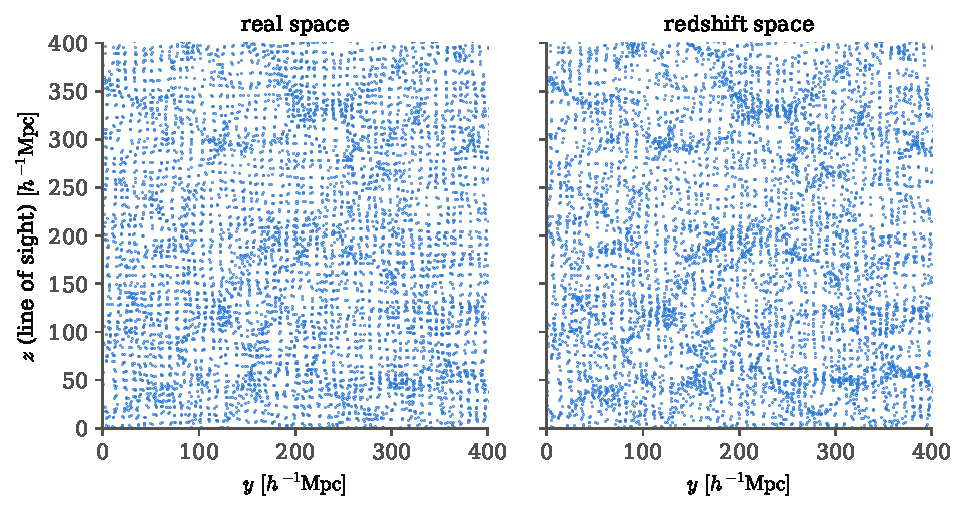
\includegraphics[width=0.95\linewidth]{figures/ch11/rsd_slice.pdf}
\caption{A slab $20\,h^{-1}$Mpc thick from one Zel'dovich box at $z=\RsdZ$, in real
space (left) and redshift space (right), with the line of sight vertical. The
faint grid pattern is the starting lattice, not yet erased by the small
displacements. Every particle on the right is moved vertically only, by
$f\Psi_z$. By eye the difference is slight at this amplitude; the power spectra
of \cref{11a:fig:rsd-kaiser} measure it.}
\label{11a:fig:rsd-slice}
\end{figure}

\begin{figure}[htbp]
\centering
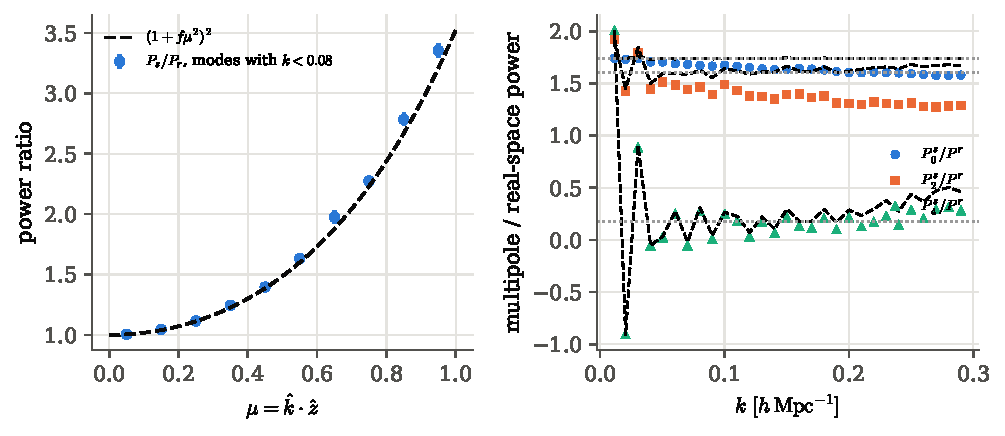
\includegraphics[width=0.95\linewidth]{figures/ch11/rsd_kaiser.pdf}
\caption{Left: the ratio of redshift-space to real-space power for modes with
$k<0.08\,h\,\mathrm{Mpc}^{-1}$, averaged in bins of $\mu$, against the Kaiser
factor $(1+f\mu^2)^2$ (dashed). Right: the monopole (blue), quadrupole (orange)
and hexadecapole (green) of the redshift-space power, each divided by the
real-space power. Dotted grey lines are the continuum Kaiser values
$1+\frac23f+\frac15f^2$, $\frac43f+\frac47f^2$ and $\frac8{35}f^2$; the black dashed
curves apply $(1+f\mu^2)^2$ to the boxes' own real-space modes and then take the
multipoles with the same discrete average.}
\label{11a:fig:rsd-kaiser}
\end{figure}

\paragraph{What the boxes show.}
The left panel of \cref{11a:fig:rsd-kaiser} follows $(1+f\mu^2)^2$ from $\mu=0$,
where the two powers agree, to $\mu=1$, where the redshift-space power is more
than three times larger. The least-squares fit gives $\hat f=\RsdFhat$ against the
input $f=\RsdF$. The scatter of $\hat f$ between boxes is $\RsdFsd$, so the mean
of $\RsdNsim$ boxes is uncertain by $\RsdFerr$; the difference
$\hat f-f=\RsdFoff$ is $\RsdFpull$ times that error, too large to be chance. What could
make the boost slightly too small? Not the linear physics, which the
derivation covers exactly, but the part of the displacements that is not
coherent on large scales. The rms Zel'dovich displacement per axis is
$\sigma_\Psi=\RsdPsi\,h^{-1}$Mpc, so the redshift-space shift $f\Psi_z$ has an rms
of $\RsdSmear\,h^{-1}$Mpc, and its small-scale part smears the field along the
line of sight much like the random shifts of \eqref{11a:eq:fog}: a finger of God
in miniature. If that is the cause, the deficit must grow with $k$ and hit the
quadrupole hardest, since the damping acts at $\mu$ near $\pm1$. At
$k=0.2\,h\,\mathrm{Mpc}^{-1}$ the exponent $(kf\sigma_\Psi)^2$ is already $\RsdDampK$, and the quadrupole in the right panel falls below the
Kaiser value there. At the small $k$ of the fit the effect is small but visible.

For the multipoles averaged over $k<0.06\,h\,\mathrm{Mpc}^{-1}$, the monopole ratio
is $\RsdRzero$, against $\RsdKzero$ from \eqref{11a:eq:kaiser-mult} and
$\RsdRzeroK$ for the Kaiser factor applied to the same discrete modes. The
quadrupole ratio is $\RsdRtwo$, against $\RsdRtwoK$ for the same discrete modes,
but $\RsdKtwo$ for the continuum formula. The measured quadrupole falls
$\RsdRtwoShort\%$ below the discrete-mode prediction, the same small shortfall
from the smearing. The two predictions differ by $\RsdRtwoKex\%$, and how much
depends on the boxes drawn, since the few modes at low $k$ carry random
amplitudes. So a measured quadrupole can land near the continuum value or far
from it by chance. The gap between the two predictions is not physics but
counting, and it is a trap.

\begin{pitfall}[Multipoles of a few modes]
The continuum results \eqref{11a:eq:kaiser-mult} assume that the directions in a
$k$ shell are spread uniformly in $\mu$. At low $k$ in a box, a shell holds a few
dozen modes, and $\mu^2=k_z^2/k^2$ takes only a handful of values set by the
integer grid (for the smallest shell, values such as $0$, $\frac15$, $\frac13$,
$\frac12$, $\frac45$, $1$). Then $\langle\mu^4\rangle$ and the Legendre averages are
not $\frac15$, $\frac13$, \dots, and even a perfect Kaiser field gives a
quadrupole far from $\frac43f+\frac47f^2$ in the first bins (the jagged dashed curves
in \cref{11a:fig:rsd-kaiser}). Always compare a measured multipole with the model
evaluated on the same modes, or with a model convolved with the survey's window,
which does the same thing for a survey (\cref{11a:sec:fkp}).
\end{pitfall}

\subsection{Comparing with the data: the growth rate from BOSS}
\label{11a:sec:rsd-boss}

\emph{Their question.} By 2016 the Baryon Oscillation Spectroscopic Survey had
measured redshifts for 1.2 million massive galaxies over $9329\,\mathrm{deg}^2$
\srcref{Alam2017}{abstract}. Besides the acoustic peak, the collaboration asked
whether structure at $z\approx0.4$--$0.6$ had grown at the rate predicted by the
$\Lambda$CDM model that fits the CMB, a test of gravity on scales of tens of
megaparsecs.

\emph{Their setup.} The galaxies were divided into three overlapping redshift
slices with effective redshifts $0.38$, $0.51$ and $0.61$. Four teams fitted the
full anisotropic clustering: the monopole and quadrupole of $\xi$ between $25$
and $150\,h^{-1}$Mpc; three $\mu$-wedges of $\xi$; the power-spectrum multipoles
$P_0$, $P_2$ up to $k=0.15\,h\,\mathrm{Mpc}^{-1}$ and $P_4$ up to $0.1$; and
power-spectrum wedges up to $0.2\,h\,\mathrm{Mpc}^{-1}$
\srcref{Alam2017}{\S7}. Each used a perturbation-theory model of the non-linear
redshift-space clustering, which reduces to \eqref{11a:eq:kaiser} on large
scales and contains a velocity damping in the spirit of \eqref{11a:eq:fog}, with
the bias, the nuisance parameters and the two dilations of \cref{11a:sec:alpha}
free, and a covariance from one to two thousand mock catalogues. The four results
were combined into one consensus value of $f\sigma_8$ per slice. The quantity compared with theory is exactly the
$f\sigma_8$ of \eqref{11a:eq:fsigma8}, because, as we derived, nothing else in the
redshift-space spectrum can be separated from the bias.

\emph{What we compute.} The prediction is $f(z)\,\sigma_8\,D(z)$ for the Planck 2018
model, with $D$ and $f$ from the linear growth equation of the cosmology notes
(\pyname{growth} in \texttt{lib\_lss.py}) and $\sigma_8$ from CAMB. The data are the
consensus values with statistical and systematic errors added in quadrature.

\begin{figure}[htbp]
\centering
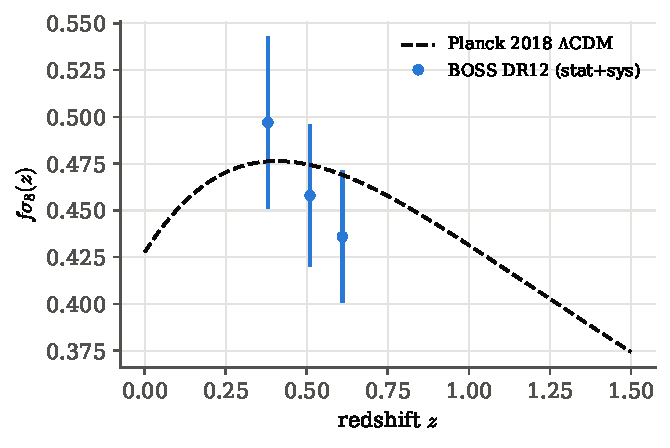
\includegraphics[width=0.62\linewidth]{figures/ch11/rsd_fsigma8.pdf}
\caption{The growth rate $f\sigma_8(z)$ of the Planck 2018 $\Lambda$CDM model
(dashed) and the BOSS DR12 consensus measurements in three redshift slices
(points, statistical and systematic errors combined; \cite{Alam2017}, Table~7).}
\label{11a:fig:rsd-fsigma8}
\end{figure}

\begin{center}
\small
\begin{tabular}{cccc}
\hline
$z_{\mathrm{eff}}$ & BOSS DR12 $f\sigma_8$ (stat, sys) & Planck $\Lambda$CDM & pull \\
\hline
$0.38$ & $0.497\pm0.039\pm0.024$ & $\RsdFsA$ & $\RsdPullA$ \\
$0.51$ & $0.458\pm0.035\pm0.015$ & $\RsdFsB$ & $\RsdPullB$ \\
$0.61$ & $0.436\pm0.034\pm0.009$ & $\RsdFsC$ & $\RsdPullC$ \\
\hline
\end{tabular}
\end{center}

\emph{Side by side.} All three points lie within one standard deviation of the
prediction (\cref{11a:fig:rsd-fsigma8}). The pulls are not three independent
draws: the slices overlap in redshift, so neighbouring measurements share
galaxies and are positively correlated, and a full test would use the published
covariance between them rather than adding three squared pulls. Even so, at
$8$--$9\%$ precision per slice, growth at $z\approx0.5$ is what $\Lambda$CDM
with the Planck parameters predicts.

\emph{The lesson.} Of the three quantities in the Kaiser formula, the survey can
deliver only the product $f\sigma_8$; once that is understood, a direction-dependent
clustering measurement becomes a test of how fast gravity builds structure.
\section{How surveys do it, and what our shortcuts cost}
\label{11a:sec:research}

Table~1 of the DESI first-year cosmology paper has one line per galaxy sample: a
redshift range, a number of objects, an effective volume and a distance ratio
such as $D_V/r_d=7.93\pm0.15$ \srcref{DESI2024VI}{Table~1}. Behind each line sits
the chain of ideas developed above: points treated as a Poisson sample of a field
(\cref{11a:sec:cox}), clustering measured against a random catalogue
(\cref{11a:sec:xi}) or through a weighted Fourier field (\cref{11a:sec:fkp}), a
template fitted for the dilation $\alpha$ (\cref{11a:sec:bao}), and the
line-of-sight squashing of \cref{11a:sec:rsd}. Our scripts ran every one of those
steps on a laptop. The survey runs each of them at full scale, on data with
real defects, with an error budget that has to survive referees who did not take
part. The question, in words:
\begin{quote}
\emph{At each step from the catalogue to a published distance or growth rate,
what does a survey do that our scaled-down versions left out, and what does
leaving it out cost?}
\end{quote}

\subsection{The pipeline of a modern survey}
\label{11a:sec:research-pipeline}

\Cref{11a:fig:research-pipeline} shows the steps. We take them in order.

\begin{figure}[htbp]
\centering
\begin{tikzpicture}[
  st/.style={draw=black!45,rounded corners=2pt,fill=formblue!7,align=center,
             font=\small,minimum height=9mm,text width=4.4cm},
  side/.style={draw=black!35,rounded corners=2pt,fill=black!3,align=center,
             font=\small,minimum height=9mm,text width=3.6cm},
  arr/.style={->,thick,black!55}]
  \node[st] (cat) at (0,0) {targets, spectra, redshifts};
  \node[st] (ran) at (0,-1.45) {catalogue and randoms:\\masks, completeness,\\weights};
  \node[st] (bli) at (0,-2.95) {blinding: shifted redshifts};
  \node[st] (rec) at (0,-4.3) {reconstruction:\\undo the bulk flows};
  \node[st] (est) at (0,-5.65) {estimators:\\LS for $\xi$, FKP for $P_\ell$};
  \node[st] (fit) at (0,-7.0) {fits: $\alpha_\parallel,\alpha_\perp$, $f\sigma_8$,\\nuisance marginalised};
  \node[st] (unb) at (0,-8.35) {tests passed $\Rightarrow$ unblind};
  \node[side] (mock) at (5.6,-4.3) {approximate mocks\\($\sim10^3$, same footprint)};
  \node[side] (nbody) at (5.6,-1.45) {$N$-body light-cone\\simulations\\(few, accurate)};
  \node[side] (cov) at (5.6,-7.0) {covariance matrix,\\error budget};
  \draw[arr] (cat) -- (ran);
  \draw[arr] (ran) -- (bli);
  \draw[arr] (bli) -- (rec);
  \draw[arr] (rec) -- (est);
  \draw[arr] (est) -- (fit);
  \draw[arr] (fit) -- (unb);
  \draw[arr] (nbody) -- (mock);
  \draw[arr] (mock) -- (cov);
  \draw[arr] (cov) -- (fit);
\end{tikzpicture}
\caption{The steps from a spectroscopic survey to a distance or growth rate (left
column) and the simulations that support them (right). Approximate mock
catalogues, calibrated on a few accurate $N$-body simulations, are run through
the same pipeline as the data; their scatter becomes the covariance matrix used
in the fits.}
\label{11a:fig:research-pipeline}
\end{figure}

\paragraph{The catalogue and its randoms.}
A real footprint is not a square with a few holes. In BOSS the veto masks, for
bright stars, poor imaging, plate centre-posts and similar defects, removed
$6.6\%$ and $9.3\%$ of the area in the two galactic caps, leaving a
completeness-weighted area of $9329\,\mathrm{deg}^2$; the galaxies carry weights
that undo the dependence of the target density on stellar density and seeing,
and corrections for fibre collisions and failed redshifts
\srcref{Alam2017}{\S2}. In DESI's first year only $35\%$ of the emission-line
galaxy targets had received a fibre \srcref{DESI2024VI}{\S2.1}. Every one of these
effects modulates the observed density without any cosmological cause. The
random catalogue of \cref{11a:sec:xi} must carry every one of them, and the
pitfall there (the randoms must have the survey's selection, exactly) is the
reason survey teams spend more effort on the randoms than on the estimator. The
FKP weights of \cref{11a:sec:fkp} multiply these systematic weights.

\paragraph{Blinding.}
\emph{The problem.} An analysis has hundreds of choices: which weights, which
range of scales, which model of the broad band. Each choice is defended by tests,
and tests are run until they pass. If the analysts can see the cosmological
answer while they work, there is a mechanism that biases the result without
anyone intending it. The DESI paper describes it plainly: a result that does not
match expectation is attributed to an unknown systematic, and the search for
systematics stops when the result agrees \srcref{DESI2024VI}{\S2.3.1}.

\emph{Why that is a statistical bias.} Think of the analysis as drawing an
estimate $\hat\theta$ from its sampling distribution. Suppose an analyst looks at
$\hat\theta$, keeps it if it lies within $2\sigma$ of the expected value, and
otherwise searches for, finds, and corrects some small effect, which redraws
part of the noise. The rule for when to stop depends on the value obtained.
The published estimates are then a sample from the sampling distribution
\emph{conditioned on agreeing with expectation}: they are pulled towards the
expected value, they scatter less than the quoted error says, and a genuine
discrepancy is the one result the procedure is built to remove. It is the same
mechanism as stopping an experiment when the $p$-value first drops below $0.05$,
run in the opposite direction.

\emph{What DESI did.} Before analysis the redshifts in the galaxy and quasar
catalogues were shifted, by an amount unknown to the analysts, in a way that
moves the acoustic feature and changes the redshift-space distortion signal, and
the weights were altered to hide the large-scale signal of primordial
non-Gaussianity. All tests were run on the blinded catalogues; only after the
pipeline was frozen and a prescribed list of validation tests had passed were
the true redshifts used. Two changes made after unblinding were reported with
their size: a correction to the BAO model, which moved the results by less than
$0.3\sigma$, and a completeness fix in the catalogues, by at most $0.6\sigma$
\srcref{DESI2024VI}{\S2.3.1}. BOSS blinded the methods rather than the data: the
four full-shape analyses of \cref{11a:sec:rsd-boss} were first run on
high-fidelity mocks whose parameters the teams did not know, and their errors
there entered the systematic budget \srcref{Alam2017}{\S7}.

\paragraph{Reconstruction.}
The acoustic peak is blurred because galaxies have moved a few megaparsecs since
the drag epoch, the damping $\Sigma_{\mathrm{nl}}$ of \cref{11a:sec:bao}. The
displacements are not random: on large scales they are the Zel'dovich field
$\bm\Psi_{\bm k}=i\bm k\,\delta_{\bm k}/k^2$ of \cref{11a:sec:rsd-python}, and the
observed galaxy field gives an estimate of $\delta$. \newterm{Reconstruction}
computes that $\bm\Psi$ from the smoothed galaxy field (divided by the bias, and
with the redshift-space term $f\Psi_z$ removed), and moves every galaxy and
random back by it \srcref{DESI2024VI}{\S2.3}. The peak sharpens, roughly halving
$\Sigma_{\mathrm{nl}}$ from $8$ to $4\,h^{-1}$Mpc \srcref{Anderson2012}{\S5.2},
and the small non-linear shift of the peak position, below $0.3\%$, is largely
undone. In the Fisher forecast of \cref{11a:sec:bao} for DESI's bright galaxies
this was the difference between $\FishDesiPre\%$ and $\FishDesiRec\%$ on $\alpha$:
halving the error is worth a factor four in survey volume, so reconstruction is
worth about as much as quadrupling the survey, at the cost of one more step to validate on mocks.

\paragraph{Estimators and fits.}
The estimators are the ones we derived: Landy--Szalay pair counts against random
catalogues many times larger than the data (\cite{Eisenstein2005} used sixteen
times as many randoms), and FKP-weighted Fourier fields, now with fast-Fourier
estimators for the multipoles $P_0$, $P_2$, $P_4$ \srcref{Alam2017}{\S7}. The BAO
fit uses a template with two dilations, $\alpha_\parallel$ and $\alpha_\perp$,
and nuisance parameters for the broad band that are marginalised over
\srcref{DESI2024VI}{\S2.3}; it is \cref{11a:sec:bao-fit} with one more dilation and
the Alcock--Paczy\'nski information of \cref{11a:sec:alpha} kept. The
theoretical systematic errors of this procedure are estimated at $0.1\%$ for the
isotropic and $0.2\%$ for the anisotropic BAO parameters, with up to $0.2\%$ more
from how galaxies populate haloes; they are added in quadrature to the
statistical error \srcref{DESI2024VI}{\S2.3}.

\paragraph{Mocks for the covariance.}
Every fit needs the covariance matrix of the measured $\xi$ or $P_\ell$. The
Gaussian formula of \cref{11a:sec:fkp} is not trusted for this: in
\cref{11a:sec:fkp-python} the scatter of the lognormal field already exceeded it by
a factor $\FkpExcessB$ at $k=\FkpKb\,h\,\mathrm{Mpc}^{-1}$. Surveys instead run a
thousand or more mock catalogues through the full pipeline, each with the
survey's footprint, completeness, fibre collisions and $n(z)$. Full $N$-body
simulations are too expensive at that number, so the mocks use approximate
dynamics: \citeauthor{Eisenstein2005} used 1278 PTHalos mocks, and BOSS DR12
used 1000 MultiDark-Patchy mocks (second-order Lagrangian perturbation theory
plus a stochastic model for haloes) and 1000 QPM mocks (a low-resolution
particle-mesh code), both populated with galaxies to match the observed
clustering \srcref{Alam2017}{\S4}. DESI's first-year BAO analysis used
semi-analytic covariance matrices validated against such mocks
\srcref{DESI2024VI}{\S2.3}. A few accurate $N$-body light-cone simulations
serve as the reference that the approximate mocks and the models are checked
against; one public set provides 108 full-sky realisations with haloes resolved
down to the hosts of the BOSS CMASS and luminous red galaxies
\cite{Takahashi2017sims}.

The cost of a finite number of mocks is the subject of \cref{8b:sec:hartlap}. With
$N_S$ mocks and $N_D$ data bins, the inverse of the sample covariance must be
multiplied by the Hartlap factor $(N_S-N_D-2)/(N_S-1)$
(\cref{3a:eq:hartlap}), and even then the variance of each parameter is itself
uncertain by a fraction $\varepsilon=\sqrt{2/(N_S-N_D-4)}$ (\cref{8b:sec:taylor}).
Since the error bar is the square root of the variance, its fractional scatter is
$\varepsilon/2$ by the delta method (\cref{3a:sec:delta}).

\paragraph{Example: our acoustic-peak mocks against the 2005 analysis.}
The covariance in \cref{11a:sec:bao-mocks} came from $\BaoNcov$ mocks for
$\BaoNbins$ bins: Hartlap factor $\ResOursHartlap$ and $\varepsilon=\ResOursEps\%$,
so each error bar is uncertain by $\ResOursSig\%$. The 2005 analysis, 1278 mocks
for 20 bins, had $\ResEisHartlap$ and $\ResEisSig\%$. On this count our nerfed run
is as good as the original, which is a statement about bins: a data vector of a
few tens of bins is cheap.

\paragraph{Example: a joint fit of many multipoles.}
A modern full-shape fit uses $P_0$, $P_2$, $P_4$ in several redshift bins and both
galactic caps, easily a hundred numbers. With $N_D=100$ and $1000$ mocks the
Hartlap factor is $\ResHartlapHundredK$: a $10\%$ correction to every $\chi^2$. For
an error bar good to $5\%$, \cref{8b:eq:taylor} asks for $\ResNsFiveHundred$ mocks
with $N_D=100$ against $\ResNsFiveSixteen$ with $N_D=16$. The mocks are cheap
compared with their validation; what limits a survey is not their number but
how well their clustering matches the real galaxies'.

\begin{figure}[htbp]
\centering
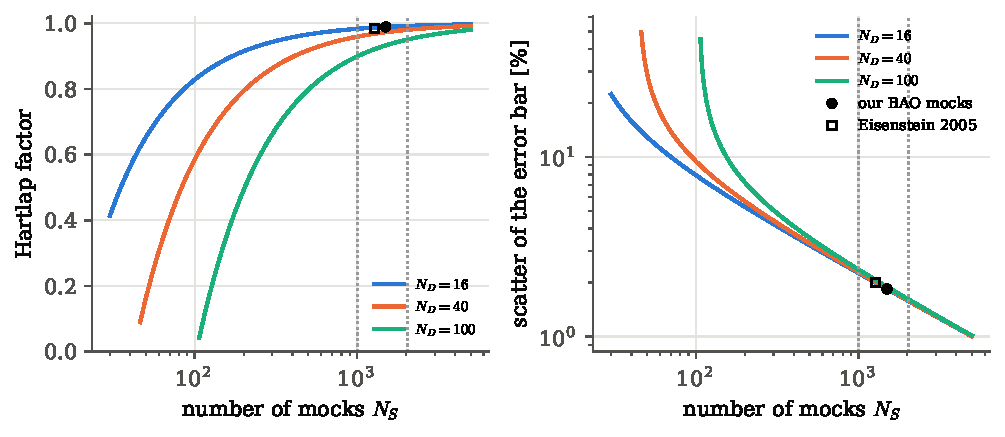
\includegraphics[width=0.95\linewidth]{figures/ch11/research_mocks.pdf}
\caption{The price of a covariance matrix estimated from $N_S$ mocks, for data
vectors of $N_D=16$, $40$ and $100$ bins. Left: the Hartlap factor that de-biases
the inverse covariance. Right: the fractional scatter of a parameter's error
bar, $\varepsilon/2$. Black points: our acoustic-peak mocks (filled) and the 2005
analysis (open). Dotted lines: the BOSS DR12 mock sets of $1000$ and $2045$.}
\label{11a:fig:research-mocks}
\end{figure}

\paragraph{Designing the survey.}
The same Fisher forecast that we checked against mocks in \cref{11a:sec:bao} is
how surveys are planned: one writes the error on the BAO distances as a function
of area, depth, redshift range and target density, and optimises it under the
constraints of the instrument, the field of view, the number of fibres and the
total observing time \srcref{HobsonBMC}{\S5.3.3}. The effective volume
$V_{\mathrm{eff}}$ of \cref{11a:sec:fkp} is the quantity being traded: more area
at fixed time means fewer galaxies per unit volume and a smaller $\bar nP$.

\subsection{What our shortcuts cost}
\label{11a:sec:research-nerfs}

Every script ran in minutes on a laptop. \Cref{11a:tab:nerfs}
lists, step by step, what the research version does instead and what the
simplification costs. Two kinds of cost appear. Some only widen error bars or
shrink the range of scales and could be removed with more computing time; the
cluster versions of the scripts would do so. Others leave a physical effect out
altogether, and no amount of computing in the same model brings it back.

\begin{table}[htbp]
\centering
\small
\begin{tabular}{p{2.0cm}p{3.6cm}p{3.6cm}p{4.0cm}}
\hline
step & research & ours & what it costs \\
\hline
density field & $N$-body or 2LPT dynamics, galaxies placed in haloes &
Gaussian and lognormal fields; Zel'dovich particles &
covariance only roughly right (scatter $\FkpExcessB\times$ Gaussian in the FKP
test); no realistic three-point function \\
geometry & light cone, true footprint and $n(z)$, curved sky &
masked 2-D square for $\xi$; sphere with $\bar n(r)$ for FKP; periodic boxes for BAO
and RSD & no window in the BAO fit; distant observer only; no evolution with
redshift inside a sample \\
mocks & $10^3$--$2\times10^3$ approximate mocks, a few $N$-body &
$\BaoNcov$ (BAO), $\XiNsim$ ($\xi$), $\FkpNsim$ (FKP), $\RsdNsim$ (RSD) &
error bars uncertain by $\ResOursSig\%$ for BAO; RSD only a verification \\
reconstruction & yes & no &
$\sigma_\alpha$ forecast $\FishDesiPre\%$ instead of $\FishDesiRec\%$ for DESI's bright
galaxies \\
BAO fit & $\alpha_\parallel$, $\alpha_\perp$, broad band marginalised &
isotropic $\alpha$ & no separate $D_M$ and $D_H$, no Alcock--Paczy\'nski
information \\
RSD model & perturbation theory with nuisance parameters, $k\lesssim0.15$--$0.2$ &
linear Kaiser on $k<0.08\,h\,\mathrm{Mpc}^{-1}$ &
$\hat f-f=\RsdFoff$ ($\RsdFpull$ errors), from the smearing; fewer modes \\
systematics & weights for stars, seeing, fibre collisions; blinding &
none & nothing in simulations, which have no systematics; fatal on real data \\
\hline
\end{tabular}
\caption{Each step of the analysis at research scale and in the
scripts, with the cost of the simplification.}
\label{11a:tab:nerfs}
\end{table}

The first row is the one that matters most and the one we can do least about on
a laptop. A lognormal field has the right one- and two-point statistics by
construction and the wrong higher-order ones. Every statement
that depends only on the two-point function, the shot noise, the estimators'
first-order behaviour, the FKP weight, the Kaiser factor, transferred correctly
from our simulations to the theory. Every statement that depends on the
four-point function, the absolute covariance and therefore the absolute error
bars, transferred only roughly. That is precisely why surveys build mocks with
realistic dynamics and why the cosmic web's higher-order structure, which the
two-point function does not see, carries information of its own, which the halo
model, voids and the topological summaries of \cref{ch:12} set out to extract.

\paragraph{The lesson.}
A survey measurement is the same short chain of estimators we derived, wrapped
in a much longer chain of corrections, simulations and checks; the estimators
fix what is measured, and the mocks and the blinding decide whether the quoted
error can be believed.

\begin{recap}
\begin{itemize}[leftmargin=1.2em,itemsep=2pt]
  \item Galaxies are modelled as a Cox process: Poisson given a smooth field
        $\bar n(1+\delta_g)$. Counts in cells have variance
        $\langle N\rangle+\langle N\rangle^2\sigma_R^2$, pairs have density
        $\bar n^2(1+\xi)$, and the power of the points is $P(k)+1/\bar n$
        (\cref{11a:sec:cox}).
  \item $\xi(r)$ is estimated by comparing data pairs with pairs of a random
        catalogue that has the survey's selection. Written to first order in the
        fluctuations, Landy--Szalay $(DD-2DR+RR)/RR$ cancels the edge terms that
        the natural and Davis--Peebles estimators keep; every estimator carries the
        integral constraint (\cref{11a:sec:xi}).
  \item The FKP estimator weights the data-minus-randoms field by
        $w=1/(1+\bar nP)$, the weight that minimises the variance of $\hat P$;
        its mean is the window-convolved spectrum plus shot noise, and its
        information is measured by $V_{\mathrm{eff}}$ (\cref{11a:sec:fkp}).
  \item The acoustic peak is a ruler of length $r_d$; fitting a template with
        dilation $\alpha$ measures $D_V/r_d$, the detection significance is
        $\sqrt{\Delta\chi^2}$ between peaked and smooth templates, and the Fisher
        forecast on $\alpha$ is a lower bound reached only at high
        signal-to-noise (\cref{11a:sec:bao}).
  \item Peculiar velocities move galaxies along the line of sight by
        $u_r/(aH)$. Number conservation and the linear continuity equation give
        $P_s(k,\mu)=(b+f\mu^2)^2P(k)$, with multipoles $P_0$, $P_2$, $P_4$ only;
        clustering alone measures $b\sigma_8$ and $f\sigma_8$, and $f\sigma_8$ is
        the growth rate of the amplitude of structure (\cref{11a:sec:rsd}).
  \item Surveys add masks, weights, blinding, reconstruction and a thousand or
        more mocks for the covariance; our laptop versions keep the estimators
        and lose the realistic covariance (\cref{11a:sec:research}).
\end{itemize}
\end{recap}
\providecommand{\SameL}{}\renewcommand{\SameL}{600}
\providecommand{\SameN}{}\renewcommand{\SameN}{192}
\providecommand{\SameR}{}\renewcommand{\SameR}{8}
\providecommand{\SamePkDev}{}\renewcommand{\SamePkDev}{2.519\times10^{-12}}
\providecommand{\SameSigZA}{}\renewcommand{\SameSigZA}{0.7111}
\providecommand{\SameSigTw}{}\renewcommand{\SameSigTw}{0.7111}
\providecommand{\SameSkewZA}{}\renewcommand{\SameSkewZA}{1.883}
\providecommand{\SameSkewTw}{}\renewcommand{\SameSkewTw}{0.01497}
\providecommand{\SameNegZA}{}\renewcommand{\SameNegZA}{0}
\providecommand{\SameNegTw}{}\renewcommand{\SameNegTw}{7.992}
\providecommand{\SameDeepZA}{}\renewcommand{\SameDeepZA}{16.4}
\providecommand{\SameDeepTw}{}\renewcommand{\SameDeepTw}{19.96}
\providecommand{\SameNvZA}{}\renewcommand{\SameNvZA}{3607}
\providecommand{\SameNvTw}{}\renewcommand{\SameNvTw}{2546}
\providecommand{\SameVfZA}{}\renewcommand{\SameVfZA}{8.482}
\providecommand{\SameVfTw}{}\renewcommand{\SameVfTw}{4.569}
\providecommand{\SameRmaxZA}{}\renewcommand{\SameRmaxZA}{23.16}
\providecommand{\SameRmaxTw}{}\renewcommand{\SameRmaxTw}{15.9}
\providecommand{\HmfNchk}{}\renewcommand{\HmfNchk}{20000}
\providecommand{\HmfSeAbove}{}\renewcommand{\HmfSeAbove}{0.0028}
\providecommand{\HmfSeCrossed}{}\renewcommand{\HmfSeCrossed}{0.0035}
\providecommand{\HmfRatioMeas}{}\renewcommand{\HmfRatioMeas}{2.058}
\providecommand{\HmfRatioMeasErr}{}\renewcommand{\HmfRatioMeasErr}{0.034}
\providecommand{\HmfNfield}{}\renewcommand{\HmfNfield}{4}
\providecommand{\HmfSharpRatioTwoErr}{}\renewcommand{\HmfSharpRatioTwoErr}{0.05}
\providecommand{\HmfTopRatioTwoErr}{}\renewcommand{\HmfTopRatioTwoErr}{0.02}
\providecommand{\HmfSharpRatioTwoSd}{}\renewcommand{\HmfSharpRatioTwoSd}{0.10}
\providecommand{\HmfNwalk}{}\renewcommand{\HmfNwalk}{50000}
\providecommand{\HmfNstep}{}\renewcommand{\HmfNstep}{4000}
\providecommand{\HmfSchk}{}\renewcommand{\HmfSchk}{4}
\providecommand{\HmfNuchk}{}\renewcommand{\HmfNuchk}{0.843}
\providecommand{\HmfAbove}{}\renewcommand{\HmfAbove}{0.1965}
\providecommand{\HmfCrossed}{}\renewcommand{\HmfCrossed}{0.4043}
\providecommand{\HmfAboveTh}{}\renewcommand{\HmfAboveTh}{0.1996}
\providecommand{\HmfCrossedTh}{}\renewcommand{\HmfCrossedTh}{0.3992}
\providecommand{\HmfChi}{}\renewcommand{\HmfChi}{23.1}
\providecommand{\HmfNbins}{}\renewcommand{\HmfNbins}{26}
\providecommand{\HmfFieldN}{}\renewcommand{\HmfFieldN}{160}
\providecommand{\HmfNuFieldMin}{}\renewcommand{\HmfNuFieldMin}{0.35}
\providecommand{\HmfTopRatioTwo}{}\renewcommand{\HmfTopRatioTwo}{1.07}
\providecommand{\HmfSharpRatioTwo}{}\renewcommand{\HmfSharpRatioTwo}{0.72}
\providecommand{\HmfNuTwo}{}\renewcommand{\HmfNuTwo}{2.475}
\providecommand{\HmfAst}{}\renewcommand{\HmfAst}{0.3222}
\providecommand{\HmfMassFracST}{}\renewcommand{\HmfMassFracST}{0.9883}
\providecommand{\HmfMstar}{}\renewcommand{\HmfMstar}{4.413}
\providecommand{\HmfRhoM}{}\renewcommand{\HmfRhoM}{8.747}
\providecommand{\HmfNuTwelve}{}\renewcommand{\HmfNuTwelve}{0.7941}
\providecommand{\HmfMfTwelvePS}{}\renewcommand{\HmfMfTwelvePS}{0.4269}
\providecommand{\HmfMfTwelveST}{}\renewcommand{\HmfMfTwelveST}{0.3125}
\providecommand{\HmfNfourteenPS}{}\renewcommand{\HmfNfourteenPS}{3.185\times10^{-5}}
\providecommand{\HmfNfourteenST}{}\renewcommand{\HmfNfourteenST}{2.805\times10^{-5}}
\providecommand{\HmfNfifteenPS}{}\renewcommand{\HmfNfifteenPS}{1.083\times10^{-7}}
\providecommand{\HmfNfifteenST}{}\renewcommand{\HmfNfifteenST}{2.435\times10^{-7}}
\providecommand{\HmfRatioFifteen}{}\renewcommand{\HmfRatioFifteen}{1.809}
\providecommand{\HmfRatioEleven}{}\renewcommand{\HmfRatioEleven}{0.7214}
\providecommand{\HmfRatioThirteen}{}\renewcommand{\HmfRatioThirteen}{0.6643}
\providecommand{\HmfSigFifteen}{}\renewcommand{\HmfSigFifteen}{0.5348}
\providecommand{\HmfSigEleven}{}\renewcommand{\HmfSigEleven}{2.891}
\providecommand{\HmMstar}{}\renewcommand{\HmMstar}{4.413}
\providecommand{\HmCstar}{}\renewcommand{\HmCstar}{9}
\providecommand{\HmDvir}{}\renewcommand{\HmDvir}{330}
\providecommand{\HmCfourteen}{}\renewcommand{\HmCfourteen}{5.999}
\providecommand{\HmUerr}{}\renewcommand{\HmUerr}{8.295\times10^{-10}}
\providecommand{\HmRvirFourteen}{}\renewcommand{\HmRvirFourteen}{0.9387}
\providecommand{\HmRsFourteen}{}\renewcommand{\HmRsFourteen}{0.1565}
\providecommand{\HmUkOneFourteen}{}\renewcommand{\HmUkOneFourteen}{0.9598}
\providecommand{\HmUkOneTwelve}{}\renewcommand{\HmUkOneTwelve}{0.9984}
\providecommand{\HmMassInt}{}\renewcommand{\HmMassInt}{0.592}
\providecommand{\HmBiasInt}{}\renewcommand{\HmBiasInt}{0.7056}
\providecommand{\HmBiasIntPS}{}\renewcommand{\HmBiasIntPS}{0.9119}
\providecommand{\HmMmin}{}\renewcommand{\HmMmin}{1.000\times10^{7}}
\providecommand{\HmBtwelve}{}\renewcommand{\HmBtwelve}{0.8707}
\providecommand{\HmBfourteen}{}\renewcommand{\HmBfourteen}{1.93}
\providecommand{\HmBfifteen}{}\renewcommand{\HmBfifteen}{4.701}
\providecommand{\HmBtwelvePS}{}\renewcommand{\HmBtwelvePS}{0.7809}
\providecommand{\HmBfifteenPS}{}\renewcommand{\HmBfifteenPS}{6.301}
\providecommand{\HmBmin}{}\renewcommand{\HmBmin}{0.6894}
\providecommand{\HmBminPS}{}\renewcommand{\HmBminPS}{0.4485}
\providecommand{\HmRatioPtZeroOne}{}\renewcommand{\HmRatioPtZeroOne}{1.022}
\providecommand{\HmRatioPtOne}{}\renewcommand{\HmRatioPtOne}{1.047}
\providecommand{\HmRatioPtThree}{}\renewcommand{\HmRatioPtThree}{0.8937}
\providecommand{\HmRatioOne}{}\renewcommand{\HmRatioOne}{0.837}
\providecommand{\HmRatioThree}{}\renewcommand{\HmRatioThree}{0.9773}
\providecommand{\HmRatioTen}{}\renewcommand{\HmRatioTen}{0.9775}
\providecommand{\HmRatioTenTwoHundred}{}\renewcommand{\HmRatioTenTwoHundred}{0.6821}
\providecommand{\HmKworst}{}\renewcommand{\HmKworst}{0.6311}
\providecommand{\HmRatioWorst}{}\renewcommand{\HmRatioWorst}{0.8007}
\providecommand{\HmKeq}{}\renewcommand{\HmKeq}{0.4957}
\providecommand{\HmOneHaloConst}{}\renewcommand{\HmOneHaloConst}{342.9}
\providecommand{\HmMlo}{}\renewcommand{\HmMlo}{4.381}
\providecommand{\HmMhi}{}\renewcommand{\HmMhi}{116}
\providecommand{\HodLMmin}{}\renewcommand{\HodLMmin}{12.8}
\providecommand{\HodSig}{}\renewcommand{\HodSig}{0.5}
\providecommand{\HodLMzero}{}\renewcommand{\HodLMzero}{12.6}
\providecommand{\HodLMone}{}\renewcommand{\HodLMone}{14}
\providecommand{\HodAlpha}{}\renewcommand{\HodAlpha}{1.1}
\providecommand{\HodNbar}{}\renewcommand{\HodNbar}{0.00116}
\providecommand{\HodFsat}{}\renewcommand{\HodFsat}{0.1287}
\providecommand{\HodBias}{}\renewcommand{\HodBias}{1.298}
\providecommand{\HodMeff}{}\renewcommand{\HodMeff}{4.112}
\providecommand{\HodGamma}{}\renewcommand{\HodGamma}{1.917}
\providecommand{\HodRzero}{}\renewcommand{\HodRzero}{7.161}
\providecommand{\HodShot}{}\renewcommand{\HodShot}{861.8}
\providecommand{\HodOneHaloConst}{}\renewcommand{\HodOneHaloConst}{462.2}
\providecommand{\HodPairsMC}{}\renewcommand{\HodPairsMC}{2.818}
\providecommand{\HodPairsTh}{}\renewcommand{\HodPairsTh}{2.818}
\providecommand{\HodPairsSE}{}\renewcommand{\HodPairsSE}{0.002864}
\providecommand{\HodNhalo}{}\renewcommand{\HodNhalo}{2000000}
\providecommand{\HodNcFourteen}{}\renewcommand{\HodNcFourteen}{0.9997}
\providecommand{\HodLamFourteen}{}\renewcommand{\HodLamFourteen}{0.9541}
\providecommand{\VdThr}{}\renewcommand{\VdThr}{-0.8}
\providecommand{\VdDv}{}\renewcommand{\VdDv}{-2.781}
\providecommand{\VdExpand}{}\renewcommand{\VdExpand}{1.71}
\providecommand{\VdDvSc}{}\renewcommand{\VdDvSc}{-2.811}
\providecommand{\VdDnlSc}{}\renewcommand{\VdDnlSc}{-0.8021}
\providecommand{\VdNwalk}{}\renewcommand{\VdNwalk}{40000}
\providecommand{\VdFracMC}{}\renewcommand{\VdFracMC}{0.3765}
\providecommand{\VdFracTh}{}\renewcommand{\VdFracTh}{0.3774}
\providecommand{\VdFracMCb}{}\renewcommand{\VdFracMCb}{0.2752}
\providecommand{\VdFracThb}{}\renewcommand{\VdFracThb}{0.276}
\providecommand{\VdDvoid}{}\renewcommand{\VdDvoid}{0.6226}
\providecommand{\VdN}{}\renewcommand{\VdN}{3607}
\providecommand{\VdRmin}{}\renewcommand{\VdRmin}{8}
\providecommand{\VdVolFrac}{}\renewcommand{\VdVolFrac}{8.482}
\providecommand{\VdRmax}{}\renewcommand{\VdRmax}{23.16}
\providecommand{\VdRmed}{}\renewcommand{\VdRmed}{9.732}
\providecommand{\VdFzero}{}\renewcommand{\VdFzero}{0.5273}
\providecommand{\VdDvZA}{}\renewcommand{\VdDvZA}{-2.13}
\providecommand{\VdDcZA}{}\renewcommand{\VdDcZA}{3}
\providecommand{\VdSvdwRatio}{}\renewcommand{\VdSvdwRatio}{2.751}
\providecommand{\VdVdnRatio}{}\renewcommand{\VdVdnRatio}{0.5502}
\providecommand{\VdGravRatioTwenty}{}\renewcommand{\VdGravRatioTwenty}{51.83}
\providecommand{\VdNws}{}\renewcommand{\VdNws}{7801}
\providecommand{\VdRmedWs}{}\renewcommand{\VdRmedWs}{14.68}
\providecommand{\VdNcompEight}{}\renewcommand{\VdNcompEight}{6414}
\providecommand{\VdNminEight}{}\renewcommand{\VdNminEight}{9318}
\providecommand{\VdNcompFive}{}\renewcommand{\VdNcompFive}{2257}
\providecommand{\VdNminFive}{}\renewcommand{\VdNminFive}{18867}
\providecommand{\VdNcompZero}{}\renewcommand{\VdNcompZero}{155}
\providecommand{\VdNminZero}{}\renewcommand{\VdNminZero}{20475}
\providecommand{\VdNcompMax}{}\renewcommand{\VdNcompMax}{6807}
\providecommand{\VdTcompMax}{}\renewcommand{\VdTcompMax}{-0.75}
\providecommand{\VdVolUnderFive}{}\renewcommand{\VdVolUnderFive}{0.2892}
\providecommand{\VdNA}{}\renewcommand{\VdNA}{1780}
\providecommand{\VdRA}{}\renewcommand{\VdRA}{11.81}
\providecommand{\VdDcA}{}\renewcommand{\VdDcA}{-0.9515}
\providecommand{\VdRsA}{}\renewcommand{\VdRsA}{1.065}
\providecommand{\VdAlA}{}\renewcommand{\VdAlA}{2.088}
\providecommand{\VdBeA}{}\renewcommand{\VdBeA}{25}
\providecommand{\VdChiA}{}\renewcommand{\VdChiA}{1.302e+04}
\providecommand{\VdDofA}{}\renewcommand{\VdDofA}{25}
\providecommand{\VdDcErrA}{}\renewcommand{\VdDcErrA}{0.00493}
\providecommand{\VdRsErrA}{}\renewcommand{\VdRsErrA}{0.01023}
\providecommand{\VdAlErrA}{}\renewcommand{\VdAlErrA}{0.05507}
\providecommand{\VdBeErrA}{}\renewcommand{\VdBeErrA}{6.187}
\providecommand{\VdAlHA}{}\renewcommand{\VdAlHA}{1.87}
\providecommand{\VdBeHA}{}\renewcommand{\VdBeHA}{7.961}
\providecommand{\VdCumThreeA}{}\renewcommand{\VdCumThreeA}{-0.1431}
\providecommand{\VdVmaxA}{}\renewcommand{\VdVmaxA}{162.7}
\providecommand{\VdVlinmaxA}{}\renewcommand{\VdVlinmaxA}{105.1}
\providecommand{\VdVzamaxA}{}\renewcommand{\VdVzamaxA}{154.4}
\providecommand{\VdWallA}{}\renewcommand{\VdWallA}{-0.08312}
\providecommand{\VdNB}{}\renewcommand{\VdNB}{3165}
\providecommand{\VdRB}{}\renewcommand{\VdRB}{14.48}
\providecommand{\VdDcB}{}\renewcommand{\VdDcB}{-0.9162}
\providecommand{\VdRsB}{}\renewcommand{\VdRsB}{0.9493}
\providecommand{\VdAlB}{}\renewcommand{\VdAlB}{2.35}
\providecommand{\VdBeB}{}\renewcommand{\VdBeB}{25}
\providecommand{\VdChiB}{}\renewcommand{\VdChiB}{3451}
\providecommand{\VdDofB}{}\renewcommand{\VdDofB}{25}
\providecommand{\VdDcErrB}{}\renewcommand{\VdDcErrB}{0.002726}
\providecommand{\VdRsErrB}{}\renewcommand{\VdRsErrB}{0.002647}
\providecommand{\VdAlErrB}{}\renewcommand{\VdAlErrB}{0.0285}
\providecommand{\VdBeErrB}{}\renewcommand{\VdBeErrB}{2.213}
\providecommand{\VdAlHB}{}\renewcommand{\VdAlHB}{2.101}
\providecommand{\VdBeHB}{}\renewcommand{\VdBeHB}{9.097}
\providecommand{\VdCumThreeB}{}\renewcommand{\VdCumThreeB}{-0.05293}
\providecommand{\VdVmaxB}{}\renewcommand{\VdVmaxB}{161.2}
\providecommand{\VdVlinmaxB}{}\renewcommand{\VdVlinmaxB}{119.1}
\providecommand{\VdVzamaxB}{}\renewcommand{\VdVzamaxB}{171.4}
\providecommand{\VdWallB}{}\renewcommand{\VdWallB}{0.01373}
\providecommand{\VdNC}{}\renewcommand{\VdNC}{2245}
\providecommand{\VdRC}{}\renewcommand{\VdRC}{17.5}
\providecommand{\VdDcC}{}\renewcommand{\VdDcC}{-0.91}
\providecommand{\VdRsC}{}\renewcommand{\VdRsC}{0.9238}
\providecommand{\VdAlC}{}\renewcommand{\VdAlC}{2.381}
\providecommand{\VdBeC}{}\renewcommand{\VdBeC}{11.08}
\providecommand{\VdChiC}{}\renewcommand{\VdChiC}{352}
\providecommand{\VdDofC}{}\renewcommand{\VdDofC}{25}
\providecommand{\VdDcErrC}{}\renewcommand{\VdDcErrC}{0.002632}
\providecommand{\VdRsErrC}{}\renewcommand{\VdRsErrC}{0.002615}
\providecommand{\VdAlErrC}{}\renewcommand{\VdAlErrC}{0.02763}
\providecommand{\VdBeErrC}{}\renewcommand{\VdBeErrC}{0.2419}
\providecommand{\VdAlHC}{}\renewcommand{\VdAlHC}{2.152}
\providecommand{\VdBeHC}{}\renewcommand{\VdBeHC}{9.347}
\providecommand{\VdCumThreeC}{}\renewcommand{\VdCumThreeC}{-0.01131}
\providecommand{\VdVmaxC}{}\renewcommand{\VdVmaxC}{193.3}
\providecommand{\VdVlinmaxC}{}\renewcommand{\VdVlinmaxC}{139.5}
\providecommand{\VdVzamaxC}{}\renewcommand{\VdVzamaxC}{200.4}
\providecommand{\VdWallC}{}\renewcommand{\VdWallC}{0.08982}
\providecommand{\VdND}{}\renewcommand{\VdND}{313}
\providecommand{\VdRD}{}\renewcommand{\VdRD}{21.31}
\providecommand{\VdDcD}{}\renewcommand{\VdDcD}{-0.9216}
\providecommand{\VdRsD}{}\renewcommand{\VdRsD}{0.9442}
\providecommand{\VdAlD}{}\renewcommand{\VdAlD}{2.618}
\providecommand{\VdBeD}{}\renewcommand{\VdBeD}{9.128}
\providecommand{\VdChiD}{}\renewcommand{\VdChiD}{38.54}
\providecommand{\VdDofD}{}\renewcommand{\VdDofD}{25}
\providecommand{\VdDcErrD}{}\renewcommand{\VdDcErrD}{0.004369}
\providecommand{\VdRsErrD}{}\renewcommand{\VdRsErrD}{0.006246}
\providecommand{\VdAlErrD}{}\renewcommand{\VdAlErrD}{0.05911}
\providecommand{\VdBeErrD}{}\renewcommand{\VdBeErrD}{0.2965}
\providecommand{\VdAlHD}{}\renewcommand{\VdAlHD}{2.112}
\providecommand{\VdBeHD}{}\renewcommand{\VdBeHD}{9.147}
\providecommand{\VdCumThreeD}{}\renewcommand{\VdCumThreeD}{-0.002524}
\providecommand{\VdVmaxD}{}\renewcommand{\VdVmaxD}{251.7}
\providecommand{\VdVlinmaxD}{}\renewcommand{\VdVlinmaxD}{181.7}
\providecommand{\VdVzamaxD}{}\renewcommand{\VdVzamaxD}{267}
\providecommand{\VdWallD}{}\renewcommand{\VdWallD}{0.1142}
\providecommand{\ApNvoid}{}\renewcommand{\ApNvoid}{1530}
\providecommand{\ApQtrue}{}\renewcommand{\ApQtrue}{1.05}
\providecommand{\ApFzero}{}\renewcommand{\ApFzero}{0.5273}
\providecommand{\ApQreal}{}\renewcommand{\ApQreal}{1.007}
\providecommand{\ApQrealErr}{}\renewcommand{\ApQrealErr}{0.009846}
\providecommand{\ApQap}{}\renewcommand{\ApQap}{1.055}
\providecommand{\ApQapErr}{}\renewcommand{\ApQapErr}{0.01172}
\providecommand{\ApQrsd}{}\renewcommand{\ApQrsd}{1.098}
\providecommand{\ApQrsdErr}{}\renewcommand{\ApQrsdErr}{0.01035}
\providecommand{\ApQboth}{}\renewcommand{\ApQboth}{1.155}
\providecommand{\ApQbothErr}{}\renewcommand{\ApQbothErr}{0.01141}
\providecommand{\ApQprod}{}\renewcommand{\ApQprod}{1.159}
\providecommand{\ApLevel}{}\renewcommand{\ApLevel}{-0.5}
\providecommand{\ApNjk}{}\renewcommand{\ApNjk}{27}
\providecommand{\ApRzero}{}\renewcommand{\ApRzero}{1.134}
\providecommand{\ApQrsdLin}{}\renewcommand{\ApQrsdLin}{1.141}
\providecommand{\ApQrsdZA}{}\renewcommand{\ApQrsdZA}{1.219}
\providecommand{\ApQcontZA}{}\renewcommand{\ApQcontZA}{1.086}
\providecommand{\ApQcontLin}{}\renewcommand{\ApQcontLin}{1.079}
\providecommand{\ApParZA}{}\renewcommand{\ApParZA}{1.158}
\providecommand{\ApPerpZA}{}\renewcommand{\ApPerpZA}{1.066}
\providecommand{\ApParLin}{}\renewcommand{\ApParLin}{1.131}
\providecommand{\ApPerpLin}{}\renewcommand{\ApPerpLin}{1.049}
\providecommand{\ApParMeas}{}\renewcommand{\ApParMeas}{1.116}
\providecommand{\ApPerpMeas}{}\renewcommand{\ApPerpMeas}{1.043}
\providecommand{\ApQapPct}{}\renewcommand{\ApQapPct}{1.1}
\providecommand{\ApZ}{}\renewcommand{\ApZ}{0.51}
\providecommand{\ApDMH}{}\renewcommand{\ApDMH}{0.5937}
\providecommand{\ApDlnqDom}{}\renewcommand{\ApDlnqDom}{0.3431}
\providecommand{\ApSigOm}{}\renewcommand{\ApSigOm}{0.03254}
\providecommand{\ApDMHHam}{}\renewcommand{\ApDMHHam}{0.588}
\providecommand{\ApDMHHamErr}{}\renewcommand{\ApDMHHamErr}{0.004}
 
\section{Two universes with one power spectrum}
\label{11b:sec:same}

In \cref{7a:sec:phases} we took a map of thin rings, kept the amplitude
$|\delta_{\bm k}|$ of every Fourier mode, replaced every phase by a random number,
and transformed back. The power spectrum did not change at all, and the rings
became featureless noise. That map was a toy. The matter in the real Universe
is not a toy: gravity has spent thirteen billion years pulling it into compact
clumps, stretching it into filaments and emptying the space between them. If we
play the same trick on an evolved matter field, how much of what gravity built
does the power spectrum keep?

The answer decides how much of the rest of the chapter can be done with $\xi(r)$
and $P(k)$ alone. The BAO and RSD measurements of \cref{11a:sec:bao,11a:sec:rsd}
use the two-point function on large scales, where the field is nearly Gaussian
and the power spectrum is, by \cref{7a:sec:grf}, a complete description. On the
scales of galaxies and clusters that is no longer true. The power spectrum answers
exactly one question, how strongly the fluctuation at one place is tied to the
fluctuation at a place a distance $r$ away, and whatever else the field holds is
invisible to it. The question becomes concrete:
\begin{quote}
\emph{Two matter fields have exactly the same power spectrum. In what measurable
ways can they still differ, and which physical structures carry the
difference?}
\end{quote}

\subsection{The experiment}
\label{11b:sec:same-experiment}

We need an evolved field we can make on a laptop. The Zel'dovich approximation of
\eqref{11a:eq:zeldovich} is the simplest: put one particle at the centre of every
cell of a regular grid (its Lagrangian position $\bm q$) and move it by the
displacement $\bm\Psi(\bm q)$ that linear theory predicts for today,
$\bm\Psi_{\bm k}=i\bm k\,\delta_{\bm k}/k^2$, with $\delta_{\bm k}$ drawn from the
CAMB linear spectrum at $z=0$. The script \pyname{08_same_spectrum.py} does this
for $\SameN^3$ particles in a periodic box of side $\SameL\,h^{-1}$Mpc and
deposits them on the grid with cloud-in-cell weights, which gives the density
$1+\delta(\bm x)$ of the \emph{Zel'dovich universe}. Particles that started in a
slightly overdense patch converge, those in an underdense patch diverge, and the
result already shows sheets, filaments and empty regions (\cref{11b:fig:same},
left).

The \emph{twin} is built from it exactly as in \cref{7a:sec:phases}. Fourier
transform $\delta$, keep $|\delta_{\bm k}|$, take the phases from the transform of
fresh white noise (which makes them uniformly random and keeps the reality
condition), and transform back. The ratio of the two power spectra, mode by mode,
differs from one by at most $\SamePkDev$, which is the rounding error of the
FFT. Any analysis that measures only $P(k)$ would call the two fields the same
universe. \Cref{11b:fig:same} shows that they are not.

\begin{figure}[htbp]
\centering
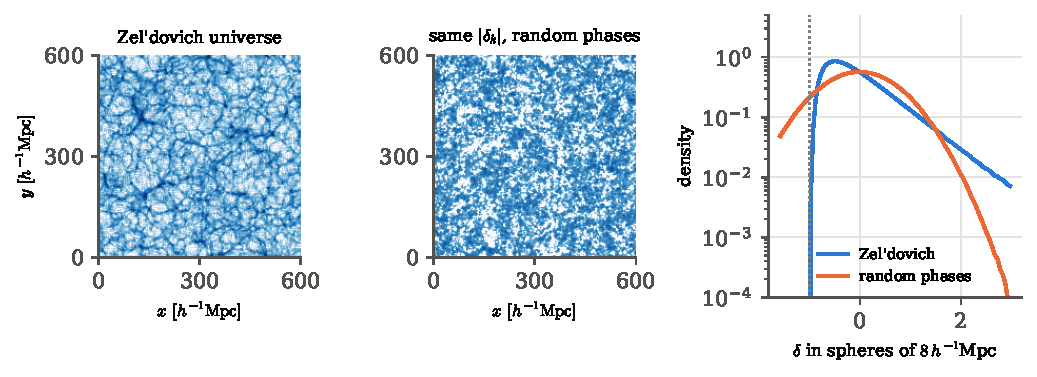
\includegraphics[width=\linewidth]{figures/ch11/same_spectrum.pdf}
\caption{Left: a slice $9\,h^{-1}$Mpc thick through the Zel'dovich universe,
darker where denser (logarithmic scale). Middle: the same slice of its twin, which
has the same $|\delta_{\bm k}|$ for every mode and random phases. Right: the
distribution of the density contrast averaged in spheres of radius
$\SameR\,h^{-1}$Mpc. The Zel'dovich field is bounded below by $\delta=-1$ (dotted)
and has a long tail to high densities; the twin is symmetric and spills below
$-1$.}
\label{11b:fig:same}
\end{figure}

\subsection{What the two fields share, and what they do not}
\label{11b:sec:same-numbers}

\paragraph{Example: the variance in spheres is the same.}
Average the density contrast over a sphere of radius $R$ about every point; call
the result $\delta_R$. Its variance is the number $\sigma_R^2$ we met in the
definition of $\sigma_8$ (\cref{T1a:sec:pk}). Write the sphere average as a
convolution with the normalised top hat $W_R$, whose Fourier transform is
$W(kR)=3(\sin kR-kR\cos kR)/(kR)^3$. Then
\begin{align}
  \sigma_R^2
  &\eqby{1}\Bigl\langle\Bigl|\int\frac{\dd^3k}{(2\pi)^3}\,
     \delta_{\bm k}W(kR)\,e^{i\bm k\cdot\bm x}\Bigr|^2\Bigr\rangle
   \eqby{2}\int\frac{\dd^3k}{(2\pi)^3}\,P(k)\,W(kR)^2
   \eqby{3}\int\frac{\dd k}{k}\,\frac{k^3P(k)}{2\pi^2}\,W(kR)^2 .
  \label{11b:eq:sigmaR}
\end{align}
\begin{explain}
  \item A convolution in real space is a product in Fourier space, so $\delta_R$
        is the inverse transform of $\delta_{\bm k}W(kR)$.
  \item Distinct modes are uncorrelated in a homogeneous field,
        $\langle\delta_{\bm k}\delta^*_{\bm k'}\rangle=(2\pi)^3\delta_D(\bm k-\bm k')P(k)$
        (\cref{7a:sec:wk}), so the double integral collapses to one, and the
        phases $e^{i\bm k\cdot\bm x}$ cancel against their conjugates.
  \item $P$ and $W$ depend only on $k=|\bm k|$, so the angular integral gives
        $4\pi k^2$, and $4\pi k^2\dd k/(2\pi)^3=(k^3/2\pi^2)\,\dd k/k$.
\end{explain}
Only $|\delta_{\bm k}|^2$ enters. The measured values agree: $\sigma_R=\SameSigZA$
in the Zel'dovich universe and $\SameSigTw$ in the twin, for
$R=\SameR\,h^{-1}$Mpc. Every quantity built from $P(k)$, the correlation
function, $\sigma_8$, the shot-noise-corrected FKP spectrum of \cref{11a:sec:fkp},
is identical in the two fields.

\paragraph{Example: the skewness is not.}
The third moment of $\delta_R$ involves three modes at once. Write
$\delta_{\bm k}=|\delta_{\bm k}|e^{i\varphi_{\bm k}}$; then
\begin{align}
  \langle\delta_R^3\rangle
  &\eqby{1}\int\!\!\frac{\dd^3k_1\,\dd^3k_2\,\dd^3k_3}{(2\pi)^9}\,
     W_1W_2W_3\,
     \bigl\langle\delta_{\bm k_1}\delta_{\bm k_2}\delta_{\bm k_3}\bigr\rangle\,
     e^{i(\bm k_1+\bm k_2+\bm k_3)\cdot\bm x}\nonumber\\
  &\eqby{2}\int\!\!\frac{\dd^3k_1\,\dd^3k_2}{(2\pi)^6}\,
     W_1W_2W_3\,
     \bigl\langle|\delta_{\bm k_1}||\delta_{\bm k_2}||\delta_{\bm k_3}|\,
     e^{i(\varphi_{\bm k_1}+\varphi_{\bm k_2}+\varphi_{\bm k_3})}\bigr\rangle_{\bm k_3=-\bm k_1-\bm k_2},
  \label{11b:eq:skew}
\end{align}
\begin{explain}
  \item Cube the Fourier representation of $\delta_R$, with the shorthand
        $W_i=W(k_iR)$.
  \item Homogeneity forces the three wavevectors to close into a triangle,
        $\bm k_1+\bm k_2+\bm k_3=0$ (the average of a product of modes is
        invariant under translations only if the total wavevector vanishes).
\end{explain}
In the twin every phase is independent and uniform, so
$\langle e^{i(\varphi_1+\varphi_2+\varphi_3)}\rangle=0$ for every triangle and the
third moment vanishes, up to the noise of one realisation. In the Zel'dovich
universe the phases of the three sides of a triangle are correlated, because
gravity couples modes: a dense clump is a place where many modes are in phase.
The measured skewness $\langle\delta_R^3\rangle/\sigma_R^3$ is $\SameSkewZA$ for
the Zel'dovich universe and $\SameSkewTw$ for the twin. The skewness is the
simplest number that the power spectrum cannot predict; its Fourier-space
counterpart is the bispectrum, the average over triangles in
\eqref{11b:eq:skew}.

\paragraph{Example: the twin is not even a possible density.}
A density cannot be negative, so $\delta\ge-1$ everywhere. In the Zel'dovich
universe the fraction of spheres with $\delta_R<-1$ is $\SameNegZA\%$. In the
twin it is $\SameNegTw\%$. The twin's one-point distribution is the symmetric
bell of a Gaussian, and a bell with $\sigma=\SameSigTw$ puts weight below $-1$.
The real field has to fit its whole variance into the range $\delta>-1$, so it
piles up just above $-1$, in the broad, nearly empty regions, and compensates with
a long tail of rare dense regions (\cref{11b:fig:same}, right). Where the mass
cannot go below a floor, matter that leaves a region must end up concentrated
somewhere else.

\paragraph{Example: the two fields have different voids.}
The spherical void finder of \cref{11b:sec:voids-finder} grows a sphere about
every local density minimum until the mean density inside reaches $20\%$ of the
cosmic mean, and keeps the non-overlapping spheres larger than
$8\,h^{-1}$Mpc. It returns $\SameNvZA$ voids filling $\SameVfZA\%$ of the
Zel'dovich box, the largest of radius $\SameRmaxZA\,h^{-1}$Mpc, and only
$\SameNvTw$ voids filling $\SameVfTw\%$ of the twin (with the unphysical
negative densities set to zero first), the largest of radius
$\SameRmaxTw\,h^{-1}$Mpc. Same power spectrum, half the empty volume.

\subsection{Where the extra information lives}
\label{11b:sec:same-where}

The four examples point at two places. The positive tail of the distribution is
made of compact, dense objects: the clumps in which the particles of the
Zel'dovich universe have crossed one another. In the real Universe these are
\newterm{dark matter haloes}, gravitationally bound and in rough virial
equilibrium, and every galaxy lives inside one. The broad pile-up just above
$\delta=-1$ is made of \newterm{voids}, large regions that matter has streamed out
of, which fill most of the volume. \Cref{11b:fig:cartoon} draws the two along a
line through a field.

\begin{figure}[htbp]
\centering
\begin{tikzpicture}
\begin{axis}[width=12cm,height=5.2cm,xmin=0,xmax=10,ymin=-1.35,ymax=5.4,
  axis lines=left,xlabel={position along a line},ylabel={$\delta$},
  xtick=\empty,ytick={-1,0,2,4},clip=false,
  every axis label/.style={font=\small},tick label style={font=\small}]
  \addplot[faint,dashed,domain=0:10] {0};
  \addplot[bdryred,thick,dotted,domain=0:10] {-1};
  \addplot[form,samples=500,domain=0:10]
    {-0.88 + 0.55*exp(-((x-2.1)/0.75)^2) + 4.2*exp(-((x-2.1)/0.12)^2)
     + 0.5*exp(-((x-7.2)/0.8)^2) + 2.6*exp(-((x-7.2)/0.15)^2)
     + 0.35*exp(-((x-0.2)/0.5)^2) + 0.3*exp(-((x-9.8)/0.5)^2)};
  \node[lbl,anchor=west] at (axis cs:2.35,3.6) {halo};
  \node[lbl,anchor=west] at (axis cs:7.45,2.0) {halo};
  \node[lbl] at (axis cs:4.65,-0.45) {void};
  \node[lbl,bdryred,anchor=west] at (axis cs:10.05,-1) {$\delta=-1$};
  \draw[decorate,decoration={brace,amplitude=5pt,mirror},softgray]
    (axis cs:3.2,-1.12) -- (axis cs:6.1,-1.12);
\end{axis}
\end{tikzpicture}
\caption{The two kinds of structure along a line through an evolved matter
field (a drawn cartoon, not data). Haloes are narrow and tall, reaching hundreds
of times the mean density; a void is a broad basin whose floor sits just above
the hard limit $\delta=-1$ (dotted), and which fills most of the line. A Gaussian
field with the same power spectrum would have neither.}
\label{11b:fig:cartoon}
\end{figure}

This suggests two ways forward, and both pay.
\begin{enumerate}[label=(\arabic*),itemsep=1pt]
  \item \emph{Build the field out of its structures.} If all matter sits in
        haloes, the statistics of the field follow from three properties of
        haloes: how many there are of each mass, how matter is arranged inside
        each, and how haloes cluster. This is the \newterm{halo model}. Its first
        payoff is a prediction of the non-linear $P(k)$ from linear theory plus
        these ingredients; its second is a model of how galaxies sit in haloes,
        which explains the shape of the galaxy correlation function
        (\cref{11b:sec:hmf,11b:sec:halo-inside,11b:sec:halomodel}).
  \item \emph{Count and measure the structures themselves.} The number of voids
        of each size, their average density profile and their average shape are
        summary statistics that, as the last example showed, respond to
        information the power spectrum discards. They need their own theory of
        what to expect, and their own estimators
        (\cref{11b:sec:voids,11b:sec:void-profiles}).
\end{enumerate}
In the language of the pipeline that runs through the book (physical model, field,
choice of information, summary, sampling distribution, inference), the halo
model is a better \emph{physical model} for the field on small scales, and the
void statistics are new \emph{summaries} whose distributions we have to derive.
Both use the same mathematical engine, the statistics of random walks, which is
where we start.

\begin{keyidea}[The power spectrum keeps amplitudes and throws away phases]
Two fields with identical $|\delta_{\bm k}|$ have identical $P(k)$, $\xi(r)$ and
$\sigma_R$, but can differ in their skewness, in their one-point distribution and
in the number and size of their voids. For an evolved matter field the
difference is carried by haloes, on the dense side, and by voids, on the empty
side.
\end{keyidea}
\section{How many haloes of each mass}
\label{11b:sec:hmf}

The most massive objects in the Universe are clusters of galaxies, haloes of
$10^{14}$--$10^{15}$ solar masses. They are rare: a cube $1\,h^{-1}$Gpc on a side
holds only a few hundred of the largest. Their number is extremely sensitive to
the amplitude of the initial fluctuations, because building a $10^{15}M_\odot$
object needs a large region to have been unusually dense, and unusual events in a
Gaussian field are exponentially rare. Counting clusters has therefore been a
cosmological probe since the 1970s, and the abundance of haloes of every mass is
the first ingredient of the halo model. The question, in words:
\begin{quote}
\emph{Given the linear density field, Gaussian with a known power spectrum, what
fraction of all the mass sits today in haloes with mass between $M$ and
$M+\dd M$?}
\end{quote}
This is a prediction, in the sense of \cref{ch:05}: from a hypothesis about the
initial field to the frequency of an outcome. Its answer becomes a likelihood for
cluster counts, and an input to everything else in this part.

\subsection{The inputs}
\label{11b:sec:hmf-inputs}

\emph{The field.} Let $\delta(\bm x)$ be the linear density contrast extrapolated
to today with the linear growth factor, as CAMB returns it. Smooth it with a
sphere of radius $R$; the sphere holds, at the mean density $\bar\rho$, the mass
$M=\tfrac{4\pi}{3}\bar\rho R^3$, so every smoothing scale is also a mass. The
smoothed contrast $\delta_M(\bm x)$ has variance $\sigma^2(M)$, given by
\eqref{11b:eq:sigmaR} with $R=(3M/4\pi\bar\rho)^{1/3}$. It falls as $M$ grows: in
our fiducial cosmology $\sigma=\HmfSigEleven$ for $M=10^{11}\,h^{-1}M_\odot$ and
$\sigma=\HmfSigFifteen$ for $M=10^{15}\,h^{-1}M_\odot$.

\emph{Collapse.} A spherical region whose linear contrast exceeds a critical value
$\delta_c$ has, according to the exact solution for a uniform spherical
perturbation, stopped expanding, turned around and collapsed by today. The
spherical-collapse solution belongs to cosmology and is taken from there (see the
cosmology notes); for an Einstein--de Sitter background it gives
\begin{equation}
  \delta_c=\frac35\Bigl(\frac{3\pi}{2}\Bigr)^{2/3}
  =0.6\times2.811=1.686,
  \label{11b:eq:deltac}
\end{equation}
with a very weak dependence on $\Omega_m$ that we ignore
\srcref{CooraySheth2002}{eq.~(53)}. The collapsed object settles at a mean
density a few hundred times $\bar\rho$; in an Einstein--de Sitter universe
$\Delta_{\mathrm{vir}}=18\pi^2\approx178$, and for $\Lambda$CDM today about $330$
relative to the mean matter density, which is the value we use for halo edges in
\cref{11b:sec:halo-inside}. The important property of \eqref{11b:eq:deltac} is
that it does not depend on the mass: the collapse of a uniform sphere depends only
on its density contrast, not on its size \srcref{CooraySheth2002}{p.~20}.

We now list what we assume, separating physics from mathematics, as for the
Poisson process of \cref{2a:sec:poisson-inputs}.

\emph{Physical inputs.}
\begin{enumerate}[label=(H\arabic*),leftmargin=2.6em,itemsep=1pt]
  \item The linear field is Gaussian, with the CAMB linear power spectrum.
  \item A region of mass $M$ around a point has collapsed into a halo by today
        if $\delta_M>\delta_c$ there. Collapse is spherical, so the threshold is
        the same constant for all masses.
  \item A mass element belongs to the most massive collapsed region that
        contains it. A small clump inside a large collapsed region is part of the
        large halo, not a halo of its own.
\end{enumerate}
\emph{Mathematical choice.}
\begin{enumerate}[label=(M\arabic*),leftmargin=2.6em,itemsep=1pt]
  \item The smoothing is done with a sharp filter in Fourier space (keep all
        modes with $k<k_c$, drop the rest) rather than a sphere in real space.
\end{enumerate}
(H1) is the standard inflationary initial condition, well tested by the CMB.
(H2) is an idealisation: real collapse is ellipsoidal, and its correction is the
subject of \cref{11b:sec:st}. (H3) is the rule that turns ``collapsed regions''
into a count of distinct objects. (M1) has no physics in it; it is chosen because
it makes the problem exactly solvable, and \cref{11b:sec:hmf-mc} measures what it
costs.

\subsection{Press and Schechter's count, and the missing half}
\label{11b:sec:ps}

\emph{The simplest guess.} Fix a mass $M$. By (H1), $\delta_M$ at a randomly
chosen point is Gaussian with mean zero and variance $\sigma^2(M)$. By (H2), the
point sits inside a collapsed region of mass at least $M$ if $\delta_M>\delta_c$.
Press and Schechter \cite{PressSchechter1974} identified the fraction of mass in
haloes heavier than $M$ with the fraction of points where this happens. Choosing a
point at random is choosing a mass element at random, because the linear field is
almost uniform, so
\begin{equation}
  \Prob(\delta_M>\delta_c)
  =\int_{\delta_c}^{\infty}\frac{\dd\delta}{\sqrt{2\pi}\,\sigma}\,
     e^{-\delta^2/2\sigma^2}
  =\frac12\operatorname{erfc}\Bigl(\frac{\nu}{\sqrt2}\Bigr),
  \qquad \nu\equiv\frac{\delta_c}{\sigma(M)} .
  \label{11b:eq:ps-naive}
\end{equation}
The variable $\nu$ is the threshold in units of the standard deviation: a halo of
mass $M$ is a ``$\nu$-sigma'' event. At $\nu=1$ the fraction is $0.159$, at $\nu=2$
it is $0.023$, at $\nu=3$ it is $0.0013$; this is the exponential sensitivity
of cluster counts.

\emph{What goes wrong.} Let $M\to0$. Then $\sigma\to\infty$, $\nu\to0$, and
\eqref{11b:eq:ps-naive} tends to $\tfrac12$. Half of the mass never belongs to any
halo, however small. But every mass element in a Gaussian field is, on some
scale, inside an overdense region. Where does the other half go? The points with
$\delta_M<\delta_c$ on scale $M$ include points that \emph{are} inside a collapsed
region on a larger scale $M'>M$. By (H3) they belong to a halo of mass $M'$, but
the count at scale $M$ never sees them. Press and Schechter multiplied their result
by $2$ by hand. The reason the factor is exactly $2$ became clear only when the
problem was reformulated as a random walk \cite{BCEK1991}.

\subsection{The excursion set: a random walk in smoothing scale}
\label{11b:sec:excursion}

Fix one point $\bm x$ and watch its smoothed contrast as the filter shrinks, from
infinitely large (where $\delta=0$, the mean) to infinitely small. With the sharp
filter of (M1),
\begin{equation}
  \delta(\bm x;k_c)=\int_{|\bm k|<k_c}\frac{\dd^3k}{(2\pi)^3}\,
     \delta_{\bm k}\,e^{i\bm k\cdot\bm x},
  \qquad
  S(k_c)\equiv\Var\bigl[\delta(\bm x;k_c)\bigr]
  =\int_{|\bm k|<k_c}\frac{\dd^3k}{(2\pi)^3}\,P(k).
  \label{11b:eq:sharpk}
\end{equation}
$S$ grows from $0$ as $k_c$ grows, so we may use $S$ itself as the ``time'' of the
trajectory. Large $S$ means a small smoothing scale and a small mass; we write
$S=\sigma^2(M)$ for the mass associated with each scale.

\emph{How does $\delta$ change when the filter shrinks a little?} Raising the
cut from $k_c$ to $k_c+\Delta k_c$ adds the modes in a thin shell,
\begin{align}
  \Delta\delta
  &\eqby{1}\int_{k_c<|\bm k|<k_c+\Delta k_c}\frac{\dd^3k}{(2\pi)^3}\,
      \delta_{\bm k}e^{i\bm k\cdot\bm x},\nonumber\\
  \bigl\langle\Delta\delta\,\delta(\bm x;k_c)\bigr\rangle
  &\eqby{2}0,\qquad
  \bigl\langle(\Delta\delta)^2\bigr\rangle
   \eqby{3}\int_{\text{shell}}\frac{\dd^3k}{(2\pi)^3}P(k)
   =S(k_c+\Delta k_c)-S(k_c)\equiv\Delta S .
  \label{11b:eq:increments}
\end{align}
\begin{explain}
  \item The difference of two sharp-$k$ integrals is the integral over the shell
        between them.
  \item The increment contains only modes in the shell, the old value only modes
        inside it. In a homogeneous field distinct modes are uncorrelated
        (\cref{7a:sec:wk}).
  \item The same orthogonality applied to the shell alone.
\end{explain}
For a Gaussian field, uncorrelated means independent (\cref{7a:sec:grf-fourier}).
So every step of the trajectory is a Gaussian of variance $\Delta S$, independent
of everything before it. That is the definition of Brownian motion, with $S$ as
time and $\delta=0$ at $S=0$. Taking two times $S_1<S_2$ and writing
$\delta(S_2)=\delta(S_1)+[\delta(S_2)-\delta(S_1)]$ gives, from the independence
of the bracket, $\langle\delta(S_1)\delta(S_2)\rangle=S_1=\min(S_1,S_2)$.

\begin{workdef}[excursion set, first crossing]
At a fixed point, the \newterm{excursion-set walk} is the smoothed linear contrast
$\delta(S)$ as a function of the variance $S=\sigma^2(M)$ of the filter. With a
sharp-$k$ filter it is a Brownian motion starting at $\delta(0)=0$. The point
belongs to a halo of mass $M$ if the walk \newterm{first crosses} the threshold
$\delta_c$ at $S=\sigma^2(M)$: no larger scale had collapsed, so by (H3) the
largest collapsed region around the point has mass $M$.
\emph{Operational:} the fraction of mass in haloes heavier than $M$ is the
fraction of walks that have crossed $\delta_c$ at some $S'<\sigma^2(M)$.
\end{workdef}

\emph{The question in walk language.} Out of all walks, what fraction has
reached $\delta_c$ at least once before time $S$? Press and Schechter counted only
the walks that are \emph{above} $\delta_c$ at time $S$. A walk that went above
earlier and came back down by time $S$ is also inside a halo of mass larger than
$M$, and it is missing from their count.

\paragraph{The reflection argument.}
Split the walks that have crossed by time $S$ into those that end above the
barrier and those that end below:
\begin{equation}
  \Prob(\text{crossed by }S)
  =\Prob\bigl(\delta(S)>\delta_c\bigr)
  +\Prob\bigl(\text{crossed by }S\text{ and }\delta(S)<\delta_c\bigr).
  \label{11b:eq:split}
\end{equation}
Take any walk in the second group. It touched $\delta_c$ for the first time at
some $S_1<S$. Reflect the part of the walk after $S_1$ in the line
$\delta=\delta_c$, replacing $\delta(S')$ by $2\delta_c-\delta(S')$ for
$S'>S_1$ (\cref{11b:fig:reflection}). The reflected walk ends above $\delta_c$.
Its steps after $S_1$ are the original steps with their signs flipped, and a
Gaussian step of mean zero is as likely as its negative, so the reflected walk is
exactly as probable as the original. The map is one to one, and every walk ending
above the barrier is the image of exactly one walk in the second group (reflect it
back after its own first crossing). The two groups have equal probability, and
\begin{align}
  \Prob(\text{crossed by }S)
  &\eqby{1}2\,\Prob\bigl(\delta(S)>\delta_c\bigr)
   \eqby{2}\operatorname{erfc}\Bigl(\frac{\delta_c}{\sqrt{2S}}\Bigr).
  \label{11b:eq:reflection}
\end{align}
\begin{explain}
  \item The second term of \eqref{11b:eq:split} equals the first, by the
        reflection. A walk that ends above the barrier has necessarily crossed it.
  \item $\delta(S)$ is Gaussian with variance $S$, so the first term is
        \eqref{11b:eq:ps-naive} with $\sigma^2=S$.
\end{explain}
As $S\to\infty$ the right side tends to $\operatorname{erfc}(0)=1$: every mass
element ends up in some halo. The factor of $2$ is not a fudge. It is the
contribution of the walks that went up and came back down, the cloud-in-cloud
mass that the single-scale count missed.

\begin{figure}[htbp]
\centering
\begin{tikzpicture}[x=1.45cm,y=1.05cm]
  \draw[->,faint] (0,0) -- (7.1,0) node[right,black,lbl] {$S$};
  \draw[->,faint] (0,-0.3) -- (0,3.3) node[above,black,lbl] {$\delta(S)$};
  \draw[bdryred,thick,dashed] (0,1.6) -- (7,1.6);
  \node[lbl,bdryred,anchor=east] at (0,1.6) {$\delta_c$};
  \draw[form] (0,0) -- (0.6,0.5) -- (1.2,0.2) -- (1.8,0.9) -- (2.4,1.25) -- (3.0,1.6);
  \draw[form] (3.0,1.6) -- (3.6,1.3) -- (4.2,0.8) -- (4.8,1.1) -- (5.4,0.5) -- (6.0,0.7) -- (6.6,0.3);
  \draw[fibre,dashed] (3.0,1.6) -- (3.6,1.9) -- (4.2,2.4) -- (4.8,2.1) -- (5.4,2.7) -- (6.0,2.5) -- (6.6,2.9);
  \fill[black] (3.0,1.6) circle (1.5pt);
  \draw[faint,dotted] (3.0,1.6) -- (3.0,0);
  \node[lbl,anchor=north] at (3.0,0) {$S_1$};
  \draw[faint,dotted] (6.6,0.3) -- (6.6,2.9);
  \node[lbl,anchor=north] at (6.6,0) {$S$};
  \fill[formblue] (6.6,0.3) circle (1.5pt);
  \fill[fibreorange] (6.6,2.9) circle (1.5pt);
  \node[lbl,formblue,anchor=west] at (6.7,0.3) {original};
  \node[lbl,fibreorange,anchor=west] at (6.7,2.9) {reflected};
\end{tikzpicture}
\caption{The reflection argument. A walk (blue) first reaches $\delta_c$ at $S_1$
and is below it again at $S$. Reflecting everything after $S_1$ in the barrier
gives a walk (orange) that is equally probable and ends above the barrier. Every
walk that crossed and came back is paired with one that ends above, so the walks
that have crossed by $S$ are twice those found above $\delta_c$ at $S$.}
\label{11b:fig:reflection}
\end{figure}

\paragraph{From the first-crossing distribution to the mass function.}
The fraction of walks that first cross between $S$ and $S+\dd S$ is the derivative
of \eqref{11b:eq:reflection}, $\mathcal F(S)\,\dd S$. It is cleaner in terms of
$\nu=\delta_c/\sqrt S$, so we change variable:
\begin{align}
  \mathcal F(S)
  &\eqby{1}\frac{\dd}{\dd S}\operatorname{erfc}\Bigl(\frac{\delta_c}{\sqrt{2S}}\Bigr)
   \eqby{2}\frac{2}{\sqrt\pi}\,e^{-\delta_c^2/2S}\,
     \frac{\delta_c}{2\sqrt2\,S^{3/2}}
   =\frac{\delta_c}{\sqrt{2\pi}\,S^{3/2}}\,e^{-\delta_c^2/2S},\nonumber\\
  F(\nu)
  &\eqby{3}\mathcal F(S)\Bigl|\frac{\dd S}{\dd\nu}\Bigr|
   \eqby{4}\frac{\delta_c\,\nu^3}{\sqrt{2\pi}\,\delta_c^3}\,e^{-\nu^2/2}\,
     \frac{2\delta_c^2}{\nu^3}
   =\sqrt{\frac2\pi}\,e^{-\nu^2/2}.
  \label{11b:eq:fnu}
\end{align}
\begin{explain}
  \item The first-crossing density is the rate at which the crossed fraction
        grows.
  \item $\frac{\dd}{\dd y}\operatorname{erfc}(y)=-\frac{2}{\sqrt\pi}e^{-y^2}$ with
        $y=\delta_c/\sqrt{2S}$ and $\frac{\dd y}{\dd S}=-\frac{\delta_c}{2\sqrt2}S^{-3/2}$;
        the two minus signs cancel.
  \item The same fraction of walks expressed per unit $\nu$ instead of per unit
        $S$: a density changes by the Jacobian (\cref{ch:02}).
  \item $S=\delta_c^2/\nu^2$, so $S^{-3/2}=\nu^3/\delta_c^3$ and
        $|\dd S/\dd\nu|=2\delta_c^2/\nu^3$.
\end{explain}
$F(\nu)\,\dd\nu$ is the fraction of all mass in haloes whose $\nu$ lies in
$[\nu,\nu+\dd\nu]$, and $\int_0^\infty F\,\dd\nu=1$, as it must be now that every
mass element is in a halo. It is called the \newterm{multiplicity function}, and
it is \emph{universal}: the power spectrum, the redshift and the mass have all
disappeared into $\nu$.

To turn mass fractions into numbers of haloes, note that a halo of mass $M$ holds
mass $M$. The mass per unit volume in haloes with masses in $[M,M+\dd M]$ is
$\bar\rho\,F(\nu)|\dd\nu/\dd M|\,\dd M$; dividing by $M$ counts them:
\begin{align}
  \frac{\dd n}{\dd\ln M}
  &\eqby{1}\frac{\bar\rho}{M}\,F(\nu)\,\Bigl|\frac{\dd\nu}{\dd\ln M}\Bigr|
   \eqby{2}\frac{\bar\rho}{M}\,\nu F(\nu)\,
     \Bigl|\frac{\dd\ln\sigma}{\dd\ln M}\Bigr| .
  \label{11b:eq:dndlnm}
\end{align}
\begin{explain}
  \item Haloes per unit volume per unit $\ln M$: the mass density in that range
        divided by the mass of one halo, with $\dd M=M\,\dd\ln M$.
  \item $\nu=\delta_c/\sigma$, so $\dd\ln\nu=-\dd\ln\sigma$ and
        $\dd\nu/\dd\ln M=-\nu\,\dd\ln\sigma/\dd\ln M$.
\end{explain}
This is the Press--Schechter mass function. In the notation of
\srcref{CooraySheth2002}{eqs.~(56)--(57)}, who write $\nu$ for our $\nu^2$, it reads
$m^2n/\bar\rho\;\dd m/m=\nu f(\nu)\,\dd\nu/\nu$ with
$\nu f(\nu)=\sqrt{\nu/2\pi}\,e^{-\nu/2}$; substituting $\nu\to\nu^2$ gives
$\nu F(\nu)/2$, the same thing.

\begin{pitfall}[Two meanings of $\nu$]
Papers on the mass function use $\nu=\delta_c/\sigma$ (Press--Schechter's and
ours) or $\nu=(\delta_c/\sigma)^2$ (Sheth and Tormen's, and Cooray and Sheth's).
The multiplicity ``$\nu f(\nu)$'' then differs by a factor of $2$, because
$\dd\ln\nu^2=2\,\dd\ln\nu$. Check the definition before comparing a formula or a
plot.
\end{pitfall}

\paragraph{Example: the characteristic mass and the clusters.}
The mass $M_*$ at which $\sigma(M_*)=\delta_c$, so $\nu=1$, separates common haloes
from rare ones. For our cosmology at $z=0$, $M_*=\HmfMstar\times10^{12}\,h^{-1}
M_\odot$. A Milky-Way-sized halo of $10^{12}\,h^{-1}M_\odot$ has
$\nu=\HmfNuTwelve$, and the fraction of all mass in haloes heavier than it is
$\int_\nu^\infty F\,\dd\nu'=\operatorname{erfc}(\nu/\sqrt2)=\HmfMfTwelvePS$: a bit
under half of all matter sits in haloes at least as massive as ours. For clusters
the number density follows from integrating \eqref{11b:eq:dndlnm} over $\ln M$:
$n(>10^{14})=\HmfNfourteenPS\,h^3\mathrm{Mpc}^{-3}$ and
$n(>10^{15})=\HmfNfifteenPS\,h^3\mathrm{Mpc}^{-3}$ (masses in $h^{-1}M_\odot$), so
a box $1\,h^{-1}$Gpc on a side holds about $10^9\times\HmfNfifteenPS\approx100$
haloes above $10^{15}\,h^{-1}M_\odot$, where $\sigma=\HmfSigFifteen$ and
$\nu\approx3$.

\begin{figure}[htbp]
\centering
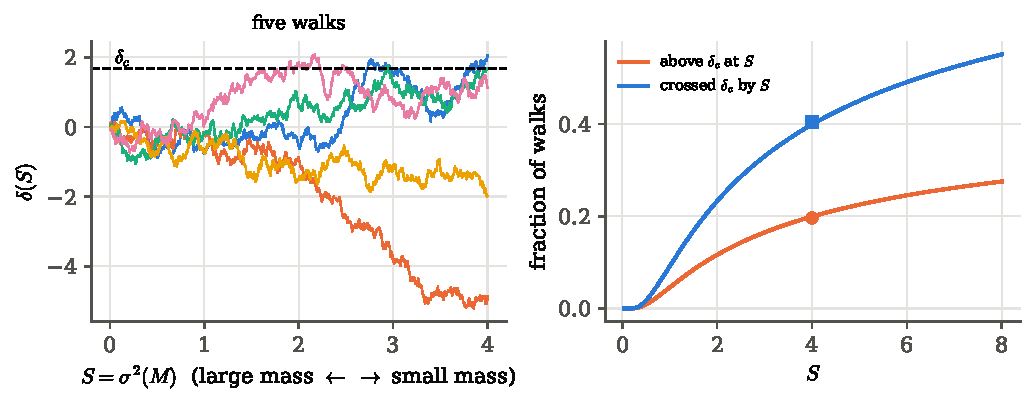
\includegraphics[width=\linewidth]{figures/ch11/hmf_walks.pdf}
\caption{Left: five excursion-set walks with independent Gaussian steps, against
the threshold $\delta_c$; moving right means smoothing on smaller scales. Right:
the fraction of walks above $\delta_c$ at $S$ (orange) and the fraction that have
crossed it at least once by $S$ (blue), with the simulated values at $S=\HmfSchk$
as points. The second curve is twice the first at every $S$.}
\label{11b:fig:hmf-walks}
\end{figure}

\subsection{Random walks on a computer}
\label{11b:sec:hmf-mc}

The reflection argument is short enough to doubt, so we simulate it.
\pyname{09_mass_function.py} draws $\HmfNwalk$ walks on a grid of $\HmfNstep$
values of $S$ between $10^{-3}$ and $60$, each step a Gaussian of variance equal to
the grid spacing, and records the first grid point at which each walk exceeds
$\delta_c$. A walk sampled only at grid points can cross the barrier and come back
between two of them unseen. For Brownian motion the probability of such a hidden
excursion is known exactly, again by reflection: between two neighbouring points
at heights $x_0,x_1<\delta_c$, separated by $\Delta S$, the walk crosses with
probability
\begin{equation}
  \frac{p_{\Delta S}(x_1-x_0\text{ via }\delta_c)}{p_{\Delta S}(x_1-x_0)}
  =\frac{e^{-(2\delta_c-x_0-x_1)^2/2\Delta S}}{e^{-(x_1-x_0)^2/2\Delta S}}
  =\exp\Bigl[-\frac{2(\delta_c-x_0)(\delta_c-x_1)}{\Delta S}\Bigr],
  \label{11b:eq:bridge}
\end{equation}
because the paths from $x_0$ to $x_1$ that touch $\delta_c$ are, after reflection
of their end, the paths from $x_0$ to $2\delta_c-x_1$, and the difference of the
two squares in the exponent is $4(\delta_c-x_0)(\delta_c-x_1)$. The function
\pyname{first_crossings} in \pyname{lib_web.py} draws this event too, which makes
the simulated crossings those of the continuous walk.

\pyfile[firstline=106,lastline=137]{code/ch11/lib_web.py}{The excursion-set walks
and their first crossings.}

The loop works in chunks of walks to keep memory small. \texttt{walk} is the
cumulative sum of the Gaussian steps; \texttt{prev} is the same walk shifted by
one point, so each pair \texttt{(prev, walk)} is one step. \texttt{hit} marks a
step where the walk is above the barrier at its end or crossed it in between
(the uniform number \texttt{u} decides the hidden crossing with probability
\eqref{11b:eq:bridge}), and \texttt{argmax} finds the first such step. The
optional lower barrier is used for voids in \cref{11b:sec:voids}.

\paragraph{The factor of 2, measured.}
At $S=\HmfSchk$ ($\nu=\HmfNuchk$) the fraction of walks above $\delta_c$ is
$\HmfAbove$, against $\tfrac12\operatorname{erfc}(\nu/\sqrt2)=\HmfAboveTh$, and the
fraction that have crossed by then is $\HmfCrossed$, against
$\operatorname{erfc}(\nu/\sqrt2)=\HmfCrossedTh$ (\cref{11b:fig:hmf-walks}, right).
This check uses $\HmfNchk$ walks, so the binomial standard error of each fraction,
$\sqrt{p(1-p)/N}$, is $\HmfSeAbove$ and $\HmfSeCrossed$. Each measured fraction
should be judged against its own error bar. The ratio of the two measured
fractions is $\HmfRatioMeas\pm\HmfRatioMeasErr$, against $2$.

\paragraph{The multiplicity function, measured.}
Histogramming $\nu=\delta_c/\sqrt{S_{\text{first}}}$ over all walks gives the
blue points of \cref{11b:fig:hmf-mult} (left), on top of
$\sqrt{2/\pi}\,e^{-\nu^2/2}$. Over the $\HmfNbins$ bins with more than fifty walks
the $\chi^2$ of the points about \eqref{11b:eq:fnu}, with Poisson errors, is
$\HmfChi$; the expected value for a correct formula is the number of bins, with a
standard deviation of about $\sqrt{2\times\HmfNbins}\approx7$. The grey dotted
curve, without the factor $2$, misses every point.

\paragraph{The same field, two filters.}
A real field is not smoothed with a sharp-$k$ filter: a halo is a region in real
space. The second experiment in the script makes $\HmfNfield$ Gaussian fields on a
$\HmfFieldN^3$ grid and reads the walk at every cell by smoothing each field
at $120$ scales, once with the sharp-$k$ filter and once with a top hat. The
error bars come from the scatter between the fields. The cells of one field are
not independent: neighbours share the same smoothed modes, so counting cells as
independent would give error bars far too small. With the
sharp-$k$ filter (green squares) the points follow Press--Schechter; at
$\nu\approx\HmfNuTwo$ they lie a factor $\HmfSharpRatioTwo\pm\HmfSharpRatioTwoErr$
below it. Part of the gap is that these
walks are read at only $120$ scales, without the correction
\eqref{11b:eq:bridge}, so crossings between two scales are missed; part is the
luck of the fields, since one field alone scatters by $\HmfSharpRatioTwoSd$ in
this ratio. With the top
hat (orange triangles) the points fall clearly below Press--Schechter at
$\nu\lesssim1.5$ and reach it, even slightly exceed it, at large $\nu$ (a factor
$\HmfTopRatioTwo\pm\HmfTopRatioTwoErr$ at $\nu\approx\HmfNuTwo$). A top hat in real space has a broad Fourier transform, so
neighbouring scales share most of their modes. The steps of the walk are then
strongly correlated, the walk is smooth, and a smooth walk rarely makes the brief
excursions above the barrier that the reflection argument pairs with the walks
ending above it. The factor of $2$ belongs to the sharp-$k$ filter; with a
realistic filter the exact first-crossing distribution has no closed form, which is
one reason the theory is calibrated on simulations
\cite{BCEK1991}.

\begin{figure}[htbp]
\centering
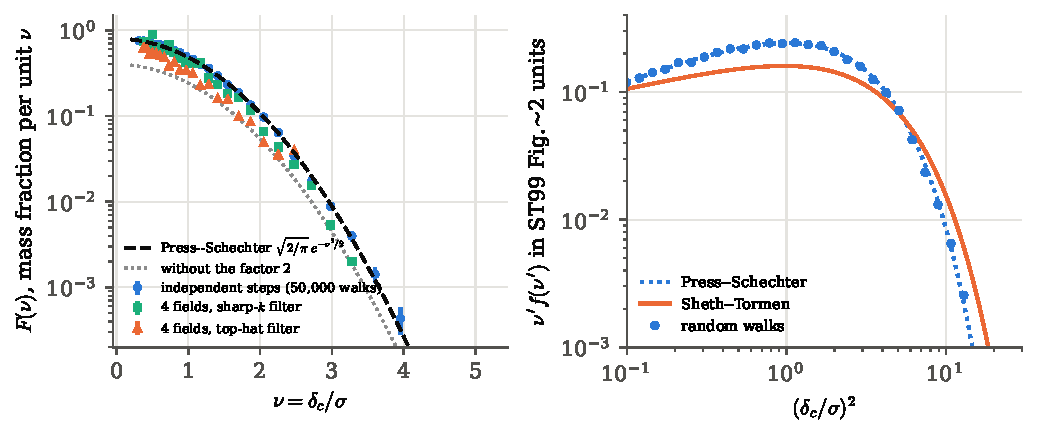
\includegraphics[width=\linewidth]{figures/ch11/hmf_multiplicity.pdf}
\caption{Left: the fraction of mass per unit $\nu$ from $\HmfNwalk$ walks with
independent steps (blue), from walks read off $\HmfNfield$ Gaussian fields with a sharp-$k$
filter (green) and a top-hat filter (orange), against Press--Schechter (dashed)
and the same formula without the factor $2$ (dotted). Right: Press--Schechter
(dotted) and Sheth--Tormen (solid) on the axes of
\srcref{ShethTormen1999}{Fig.~2}, with the random walks again as points.}
\label{11b:fig:hmf-mult}
\end{figure}

\subsection{Reproducing Sheth and Tormen}
\label{11b:sec:st}

\paragraph{Their question.}
By the late 1990s $N$-body simulations were large enough to count haloes over
four decades of mass. Press--Schechter got the shape roughly right and the
details wrong: too many small haloes and too few large ones
\srcref{CooraySheth2002}{Fig.~3}. Sheth and Tormen \cite{ShethTormen1999} asked for
a mass function that fits the simulated haloes at all masses and redshifts, and
for the halo bias that goes with it (the bias is the subject of
\cref{11b:sec:pbs}).

\paragraph{Their setup.}
They used the GIF simulations of three cold-dark-matter cosmologies, identified
haloes at several output times, and plotted the abundance against the scaled
variable $\nu_{\mathrm{ST}}=(\delta_c/\sigma)^2$, the square of ours. If the
excursion-set picture is right in spirit, the points from all times should lie on
one curve, and they did \srcref{ShethTormen1999}{Fig.~2}.

\paragraph{Their key equation.}
The curve they fitted is \srcref{ShethTormen1999}{eq.~(10)}; translated to our
$\nu=\delta_c/\sigma$ by $\nu_{\mathrm{ST}}=\nu^2$ and
$F(\nu)\,\dd\nu=f(\nu_{\mathrm{ST}})\,\dd\nu_{\mathrm{ST}}$, it reads
\begin{equation}
  F_{\mathrm{ST}}(\nu)=A\,\sqrt{\frac{2a}{\pi}}\,
  \bigl[1+(a\nu^2)^{-p}\bigr]\,e^{-a\nu^2/2},
  \qquad a=0.707,\quad p=0.3 .
  \label{11b:eq:st}
\end{equation}
The two shape parameters have direct meanings. $a<1$ stretches the exponential
cut-off to higher $\nu$, which gives more massive haloes. The bracket
$1+(a\nu^2)^{-p}$ with $p>0$ rises toward small $\nu$ as a weak power, where
Press--Schechter has a constant. Together with the smaller normalisation $A$ below
(Press--Schechter's is $\tfrac12$), the net effect over the masses that matter
for galaxies and groups is fewer haloes than Press--Schechter. The constant $A$ is not free: every mass element is in some
halo, so $\int_0^\infty F_{\mathrm{ST}}\,\dd\nu=1$. With $t=a\nu^2/2$,
\begin{align}
  \int_0^\infty F_{\mathrm{ST}}\,\dd\nu
  &\eqby{1}A\sqrt{\frac{2a}{\pi}}\int_0^\infty\bigl[1+(2t)^{-p}\bigr]
     e^{-t}\,\frac{\dd t}{\sqrt{2at}}
   \eqby{2}\frac{A}{\sqrt\pi}\Bigl[\Gamma\bigl(\tfrac12\bigr)
     +2^{-p}\,\Gamma\bigl(\tfrac12-p\bigr)\Bigr]\nonumber\\
  &\eqby{3}A\Bigl[1+\frac{2^{-p}\,\Gamma(\frac12-p)}{\sqrt\pi}\Bigr]=1
  \quad\Longrightarrow\quad
  A=\Bigl[1+\frac{2^{-p}\,\Gamma(\frac12-p)}{\sqrt\pi}\Bigr]^{-1}=\HmfAst .
  \label{11b:eq:st-norm}
\end{align}
\begin{explain}
  \item $\nu=\sqrt{2t/a}$, so $\dd\nu=\dd t/\sqrt{2at}$, and $a\nu^2=2t$.
  \item The prefactors combine to $A/\sqrt\pi$; the two terms are Gamma
        integrals, $\int_0^\infty t^{s-1}e^{-t}\dd t=\Gamma(s)$ with $s=\frac12$
        and $s=\frac12-p$.
  \item $\Gamma(\frac12)=\sqrt\pi$.
\end{explain}
For $p=0.3$, $\Gamma(0.2)=4.591$ and $2^{-0.3}=0.812$, giving the value quoted by
\srcref{CooraySheth2002}{eq.~(59)}. With $a=1$ and $p=0$ the bracket is $2$, so
$A=\frac12$ and \eqref{11b:eq:st} becomes $\frac12\sqrt{2/\pi}\,(1+1)\,e^{-\nu^2/2}$,
which is Press--Schechter: the fit contains the excursion-set result as a special
case.

\paragraph{What we compute.}
\pyname{lib_web.py} implements both multiplicities and \eqref{11b:eq:dndlnm}, with
$\sigma(M)$ from the CAMB linear spectrum; \pyname{09_mass_function.py} plots them
on Sheth and Tormen's axes, $\nu_{\mathrm{ST}}f(\nu_{\mathrm{ST}})=\nu F(\nu)/2$
against $\nu_{\mathrm{ST}}$ (\cref{11b:fig:hmf-mult}, right), and converts both to
numbers of haloes (\cref{11b:fig:hmf-nm}).

\paragraph{Side by side.}
The right panel of \cref{11b:fig:hmf-mult} reproduces the two theory curves of
their Fig.~2: Sheth--Tormen lies below Press--Schechter for
$0.05\lesssim\nu_{\mathrm{ST}}\lesssim5$ and above it beyond, by a growing
factor (it overtakes Press--Schechter again only at masses far below the range
plotted). In numbers
of haloes at $z=0$ (\cref{11b:fig:hmf-nm}), Sheth--Tormen predicts
$\HmfRatioEleven$ times as many haloes as Press--Schechter at
$10^{11}\,h^{-1}M_\odot$, $\HmfRatioThirteen$ times as many at $10^{13}$, and
$\HmfRatioFifteen$ times as many at $10^{15}$. Above $10^{15}\,h^{-1}M_\odot$ it
gives $\HmfNfifteenST\,h^3\mathrm{Mpc}^{-3}$ against $\HmfNfifteenPS$, about
$240$ instead of $100$ such clusters per $(h^{-1}\mathrm{Gpc})^3$. The mass in
haloes above $10^{12}\,h^{-1}M_\odot$ drops from $\HmfMfTwelvePS$ to
$\HmfMfTwelveST$ of the total.

\paragraph{Why they differ.}
Each difference has one cause: input (H2). Real perturbations are triaxial, and a
triaxial region feels the tidal pull of its surroundings, which resists collapse
along the longest axis. Small haloes come from regions with large $\sigma$, where
tides are relatively strong; they need a higher linear contrast than $\delta_c$
to collapse, so there are fewer of them. Massive haloes come from rare, high
peaks, which are nearly spherical and collapse almost as the spherical model
says. In walk language, ellipsoidal collapse replaces the flat barrier $\delta_c$
by one that rises with $S$, a \emph{moving barrier}. Sheth and Tormen pointed to
this explanation \srcref{ShethTormen1999}{\S4}, and the first crossings of such a
barrier were later shown to reproduce the shape of \eqref{11b:eq:st}
\cite{ShethMoTormen2001}. The random walks themselves cannot tell us this:
they verify the mathematics of (H1)--(H3), and the simulations test (H2).

\paragraph{The lesson.}
The Press--Schechter factor of $2$ is the cloud-in-cloud mass, recovered exactly
by the first-crossing problem; what remains between Press--Schechter and the
simulations, a factor of two at the extremes, is the physics of non-spherical
collapse.

\begin{figure}[htbp]
\centering
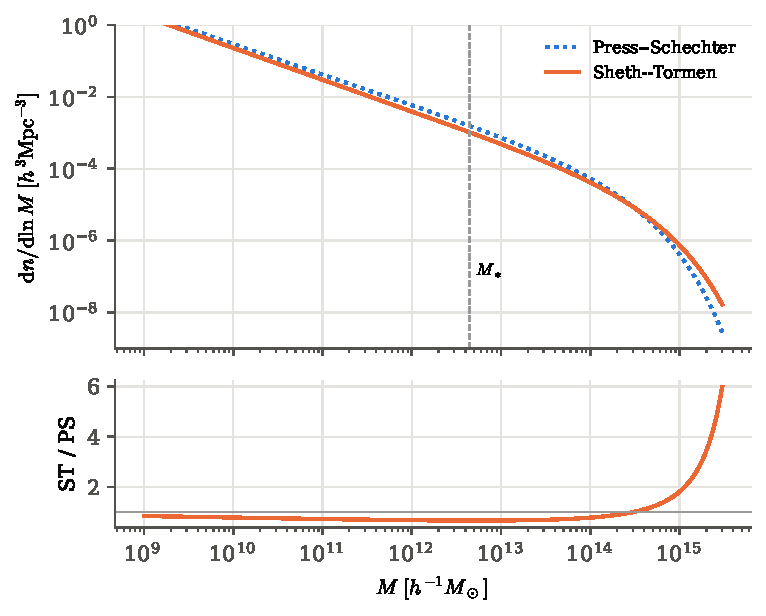
\includegraphics[width=0.78\linewidth]{figures/ch11/hmf_nM.pdf}
\caption{Haloes per unit volume per unit $\ln M$ at $z=0$ in the fiducial
cosmology, from \eqref{11b:eq:dndlnm} with the Press--Schechter (dotted) and
Sheth--Tormen (solid) multiplicities; the dashed line marks $M_*$. Lower panel:
their ratio. The abundance falls exponentially beyond $M_*$, and there the two
formulas differ most.}
\label{11b:fig:hmf-nm}
\end{figure}

\begin{keyidea}[The halo mass function from first crossings]
With a sharp-$k$ filter the smoothed linear contrast at a point is a Brownian
motion in $S=\sigma^2(M)$. The fraction of mass in haloes of mass $M$ is the
fraction of walks that first cross $\delta_c$ at $S=\sigma^2(M)$; by reflection it
is twice the naive Press--Schechter fraction, and
$\dd n/\dd\ln M=(\bar\rho/M)\,\nu F(\nu)\,|\dd\ln\sigma/\dd\ln M|$ with
$F=\sqrt{2/\pi}\,e^{-\nu^2/2}$. Simulations prefer the Sheth--Tormen form
\eqref{11b:eq:st}, the signature of ellipsoidal collapse.
\end{keyidea}
\section{Inside and around a halo}
\label{11b:sec:halo-inside}

The mass function of \cref{11b:sec:hmf} tells us how many haloes there are of
each mass. To build a density field out of haloes we need two more facts, one for
each end of the range of scales. On small scales, inside one halo, the field is
the halo's own density profile: how is the mass arranged between its centre and
its edge? On large scales, the field is made by how haloes are placed relative to
one another: do they follow the matter, or do they cluster more strongly? In
words, the two questions are:
\begin{enumerate}[label=(\arabic*),itemsep=1pt]
  \item \emph{How is the mass of a halo of mass $M$ spread around its centre, and
        what does that look like to a Fourier mode of wavenumber $k$?}
  \item \emph{If a large region is slightly denser than average, by how much does
        its number of haloes of mass $M$ go up?}
\end{enumerate}

\subsection{The density profile of a halo}
\label{11b:sec:nfw}

$N$-body haloes of all masses, in all the cold-dark-matter cosmologies that have
been simulated, have nearly the same spherically averaged profile
\cite{NFW1997},
\begin{equation}
  \rho(r\given M)=\frac{\rho_s}{(r/r_s)\,(1+r/r_s)^2},
  \label{11b:eq:nfw}
\end{equation}
the \newterm{NFW profile}. It falls as $r^{-1}$ well inside the scale radius $r_s$
and as $r^{-3}$ well outside it. There is no complete derivation of this shape
from first principles; it is a description of what simulations produce
\srcref{CooraySheth2002}{p.~34}. We take it as an input.

\emph{Where does a halo end?} The $r^{-3}$ tail would hold an infinite mass, so
the profile must be cut. We cut it at the radius $r_{\mathrm{vir}}$ inside which
the mean density is $\Delta_{\mathrm{vir}}=\HmDvir$ times the mean matter density,
the virialised density of the spherical-collapse model for $\Lambda$CDM today
(\cref{11b:sec:hmf-inputs}):
$M=\frac{4\pi}{3}\,\HmDvir\,\bar\rho\,r_{\mathrm{vir}}^3$. The ratio
$c=r_{\mathrm{vir}}/r_s$ is the \newterm{concentration}. Simulated haloes of lower
mass are more concentrated, because they formed earlier, when the Universe was
denser, and on average
\begin{equation}
  c(M)=\HmCstar\,\Bigl(\frac{M}{M_*}\Bigr)^{-0.13}
  \label{11b:eq:conc}
\end{equation}
at $z=0$, with a log-normal scatter of about $0.25$ in $\ln c$ that we ignore
\srcref{CooraySheth2002}{eqs.~(77)--(78)}.

\emph{How much mass is inside a radius?} Integrate the profile in shells, with
$x=r/r_s$:
\begin{align}
  M(<r)
  &\eqby{1}\int_0^r4\pi r'^2\rho(r')\,\dd r'
   \eqby{2}4\pi\rho_sr_s^3\int_0^{r/r_s}\frac{x\,\dd x}{(1+x)^2}
   \eqby{3}4\pi\rho_sr_s^3\Bigl[\ln(1+x)+\frac1{1+x}\Bigr]_0^{r/r_s}\nonumber\\
  &\eqby{4}4\pi\rho_sr_s^3\,m\!\left(\frac{r}{r_s}\right),
  \qquad m(y)\equiv\ln(1+y)-\frac{y}{1+y} .
  \label{11b:eq:nfw-mass}
\end{align}
\begin{explain}
  \item The mass of a thin shell is its area times its thickness times the
        density.
  \item Substitute $r'=r_sx$; then $r'^2\rho\,\dd r'=r_s^3\rho_s\,x^2\dd x/[x(1+x)^2]$.
  \item Write $x/(1+x)^2=1/(1+x)-1/(1+x)^2$ and integrate each term.
  \item At $x=0$ the bracket is $1$; subtracting it gives
        $\ln(1+y)+1/(1+y)-1=\ln(1+y)-y/(1+y)$.
\end{explain}
The total mass is $M=4\pi\rho_sr_s^3\,m(c)$ \srcref{CooraySheth2002}{eq.~(76)}, so
a halo is fixed completely by $M$: $M$ gives $r_{\mathrm{vir}}$, \eqref{11b:eq:conc}
gives $c$ and hence $r_s$, and $M=4\pi\rho_sr_s^3m(c)$ gives $\rho_s$.

\paragraph{Example: a group of $10^{14}\,h^{-1}M_\odot$.}
Here $c=\HmCfourteen$, $r_{\mathrm{vir}}=\HmRvirFourteen\,h^{-1}$Mpc and
$r_s=\HmRsFourteen\,h^{-1}$Mpc. The fraction of the mass inside $r_s$ is
$m(1)/m(c)=(\ln2-\frac12)/(\ln7-\frac67)=0.193/1.089=0.18$: less than a fifth of
the mass, in less than $1/c^3=0.5\%$ of the volume. The characteristic density
follows from equating the two expressions for $M$,
$\frac{4\pi}{3}\HmDvir\bar\rho\,c^3r_s^3=4\pi\rho_sr_s^3m(c)$, so
$\rho_s/\bar\rho=(\HmDvir/3)\,c^3/m(c)\approx2.2\times10^4$.

\subsection{A halo as seen by a Fourier mode}
\label{11b:sec:ukm}

Power spectra are built from Fourier modes, so we need the transform of the
profile. Normalise it by the mass, so that it describes the shape alone:
\begin{equation}
  u(\bm k\given M)=\frac1M\int\dd^3x\,\rho(\bm x\given M)\,e^{-i\bm k\cdot\bm x}.
  \label{11b:eq:u-def}
\end{equation}
For a spherical profile only $k=|\bm k|$ matters. Put $\bm k$ along the polar axis,
so $\bm k\cdot\bm x=kr\cos\theta$:
\begin{align}
  u(k\given M)
  &\eqby{1}\frac1M\int_0^{r_{\mathrm{vir}}}r^2\rho(r)\,\dd r
     \int_0^{2\pi}\!\dd\phi\int_{-1}^{1}e^{-ikr\mu}\,\dd\mu
   \eqby{2}\frac1M\int_0^{r_{\mathrm{vir}}}4\pi r^2\rho(r)\,
     \frac{\sin kr}{kr}\,\dd r .
  \label{11b:eq:u-radial}
\end{align}
\begin{explain}
  \item Spherical coordinates, with $\mu=\cos\theta$ and
        $\dd^3x=r^2\dd r\,\dd\phi\,\dd\mu$.
  \item $\int_{-1}^1e^{-ikr\mu}\dd\mu=(e^{ikr}-e^{-ikr})/(ikr)=2\sin(kr)/(kr)$,
        and the $\phi$ integral gives $2\pi$.
\end{explain}
Two limits are visible at once. For $k\,r_{\mathrm{vir}}\ll1$,
$\sin(kr)/(kr)\approx1-k^2r^2/6$, so $u\approx1-k^2\langle r^2\rangle/6$: a mode much
longer than the halo sees a point mass, $u\to1$. For $k\,r_s\gg1$ the factor
$\sin(kr)/(kr)$ oscillates rapidly and $u$ falls: the mode resolves the halo and
averages over its interior.

\emph{The NFW transform in closed form.} With $x=r/r_s$, $\kappa=kr_s$ and
$4\pi\rho_sr_s^3/M=1/m(c)$ from \eqref{11b:eq:nfw-mass},
\begin{align}
  u(k\given M)
  &\eqby{1}\frac{1}{m(c)\,\kappa}\int_0^c\frac{\sin\kappa x}{(1+x)^2}\,\dd x
   \eqby{2}\frac{1}{m(c)\,\kappa}\Bigl\{\Bigl[-\frac{\sin\kappa x}{1+x}\Bigr]_0^c
     +\kappa\int_0^c\frac{\cos\kappa x}{1+x}\,\dd x\Bigr\}\nonumber\\
  &\eqby{3}\frac{1}{m(c)}\Bigl\{-\frac{\sin c\kappa}{(1+c)\kappa}
     +\int_{\kappa}^{(1+c)\kappa}\frac{\cos(t-\kappa)}{t}\,\dd t\Bigr\}\nonumber\\
  &\eqby{4}\frac{1}{m(c)}\Bigl\{\sin\kappa\,\bigl[\mathrm{Si}((1+c)\kappa)-\mathrm{Si}(\kappa)\bigr]
     +\cos\kappa\,\bigl[\mathrm{Ci}((1+c)\kappa)-\mathrm{Ci}(\kappa)\bigr]
     -\frac{\sin c\kappa}{(1+c)\kappa}\Bigr\}.
  \label{11b:eq:u-nfw}
\end{align}
\begin{explain}
  \item Insert \eqref{11b:eq:nfw} into \eqref{11b:eq:u-radial}:
        $4\pi r^2\rho\,\dd r/M=x^2\,\dd x/[m(c)\,x(1+x)^2]$, and
        $\sin(kr)/(kr)=\sin(\kappa x)/(\kappa x)$; one $x$ cancels.
  \item Integrate by parts, with $(1+x)^{-2}=\frac{\dd}{\dd x}[-(1+x)^{-1}]$.
  \item The boundary term at $x=0$ vanishes. In the integral substitute
        $t=\kappa(1+x)$, so $\kappa x=t-\kappa$ and
        $\dd x/(1+x)=\dd t/t$.
  \item $\cos(t-\kappa)=\cos t\cos\kappa+\sin t\sin\kappa$, and
        $\int\sin t/t\,\dd t$ and $\int\cos t/t\,\dd t$ are the sine and cosine
        integrals, $\mathrm{Si}(y)=\int_0^y\sin t/t\,\dd t$ and
        $\mathrm{Ci}(y)=-\int_y^\infty\cos t/t\,\dd t$.
\end{explain}
This is \srcref{CooraySheth2002}{eq.~(81)}. \pyname{lib_web.py} evaluates it with
\texttt{scipy.special.sici}:

\pyfile[firstline=147,lastline=170]{code/ch11/lib_web.py}{The halo edge, the
concentration and the NFW transform.}

\noindent
\texttt{r\_halo} inverts $M=\frac{4\pi}{3}\Delta\bar\rho r^3$; \texttt{u\_nfw} builds
$r_s=r_{\mathrm{vir}}/c$, $\kappa=kr_s$, and returns the bracket of
\eqref{11b:eq:u-nfw} divided by $m(c)$, for a whole grid of masses and wavenumbers
at once. \pyname{10_halo_model.py} checks it against the integral
\eqref{11b:eq:u-radial} done numerically for $M=10^{14}\,h^{-1}M_\odot$ at three
wavenumbers; the largest relative difference is $\HmUerr$.

\paragraph{Example: when does a mode see inside a halo?}
At $k=1\,h\,\mathrm{Mpc}^{-1}$, $u=\HmUkOneFourteen$ for the group of the
previous example and $u=\HmUkOneTwelve$ for a $10^{12}\,h^{-1}M_\odot$ halo. A mode
of wavelength $2\pi/k\approx6\,h^{-1}$Mpc is still long compared with either
halo, and both look nearly like points. \Cref{11b:fig:uk-bias} (left) shows that
$u$ drops below $\frac12$ at $k\approx2\,h\,\mathrm{Mpc}^{-1}$ for
$10^{15}\,h^{-1}M_\odot$, at $k\approx4$ for $10^{14}$ and only near $k\approx50$
for $10^{11}$: the
smallest scales are resolved inside the smallest haloes, which therefore control
the power at the largest $k$ \srcref{CooraySheth2002}{Fig.~9}.

\begin{figure}[htbp]
\centering
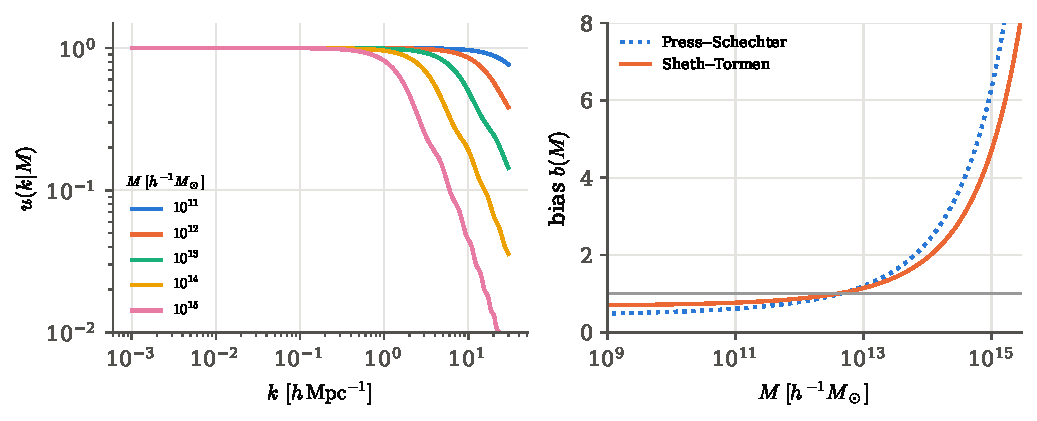
\includegraphics[width=\linewidth]{figures/ch11/halo_uk_bias.pdf}
\caption{Left: the normalised Fourier transform $u(k\given M)$ of NFW haloes with
the concentrations \eqref{11b:eq:conc}, for five masses. Each curve is $1$ for
modes longer than the halo and falls once the mode resolves its interior; heavier
haloes are larger and fall at smaller $k$. Right: the large-scale bias of haloes
from the peak-background split with the Press--Schechter (dotted) and
Sheth--Tormen (solid) mass functions. Haloes much heavier than
$M_*=\HmfMstar\times10^{12}\,h^{-1}M_\odot$ are several times more clustered than
the matter.}
\label{11b:fig:uk-bias}
\end{figure}

\subsection{Where haloes sit: the peak-background split}
\label{11b:sec:pbs}

Clusters of galaxies are far more strongly clustered than galaxies, and galaxies
more than the dark matter. The excursion set explains why, with no new input.
Picture the linear density as a sum of a long wave, the \emph{background}, and
short-wavelength ripples on top of it (\cref{11b:fig:pbs}). Haloes form where the
total crosses $\delta_c$. Where the background is high, the ripples need to climb
less far, and the threshold is crossed more often; where it is low, hardly ever.
Haloes therefore end up concentrated where the long wave is high: their number
density is modulated by the large-scale density, and modulated more strongly than
the matter is. That is \newterm{halo bias}.

\begin{figure}[htbp]
\centering
\begin{tikzpicture}
\begin{axis}[width=12cm,height=4.8cm,xmin=0,xmax=10,ymin=-1.6,ymax=1.9,
  axis lines=left,xlabel={position},ylabel={linear $\delta$},xtick=\empty,
  ytick=\empty,clip=false,every axis label/.style={font=\small}]
  \addplot[bdryred,thick,dashed,domain=0:10] {1.1};
  \addplot[fibre,thick,dashed,samples=200,domain=0:10] {0.7*cos(deg(2*pi*(x-2.5)/10))};
  \addplot[form,samples=800,domain=0:10]
     {0.7*cos(deg(2*pi*(x-2.5)/10)) + 0.42*sin(deg(2*pi*x/0.8)) + 0.22*sin(deg(2*pi*x/0.47+1.3))};
  \node[lbl,bdryred,anchor=west] at (axis cs:10.05,1.1) {$\delta_c$};
  \node[lbl,fibreorange,anchor=west] at (axis cs:10.05,0.0) {background $\delta_\ell$};
  \node[lbl,formblue,anchor=south,align=center] at (axis cs:7.5,1.4) {background low:\\ no crossings};
  \node[lbl,formblue,anchor=south,align=center] at (axis cs:2.5,1.4) {background high:\\ many crossings};
\end{axis}
\end{tikzpicture}
\caption{The peak-background split. The linear field (blue) is a long wave, the
background $\delta_\ell$ (orange), plus short ripples. The ripples are statistically
the same everywhere, but they reach the collapse threshold $\delta_c$ only where
the background lifts them; haloes form there, so their number follows the long wave
with an amplified amplitude.}
\label{11b:fig:pbs}
\end{figure}

\emph{The question in walk language.} Consider a large region, of Lagrangian
volume $V$, whose linear contrast smoothed on its own scale is $\delta_\ell$. Its
variance on that scale is $S_\ell=\sigma^2(\bar\rho V)$, small because the region is
large. Every walk starting from a point inside it passes through
$(S_\ell,\delta_\ell)$. How many of these walks first cross $\delta_c$ at the much
larger $S=\sigma^2(M)$ of a small halo?

\emph{Move the origin.} From $(S_\ell,\delta_\ell)$ onwards the walk is again a
Brownian motion, independent of its past. Measured from that point, it has to
climb $\delta_c-\delta_\ell$ in time $S-S_\ell$. For $S_\ell\ll S$ the time is
$\approx S$, and the problem is the one we solved with $\delta_c$ replaced by
$\delta_c-\delta_\ell$ \srcref{CooraySheth2002}{eq.~(63)}, \srcref{Bernardeau2002}{eqs.~(550)--(551)}.
The number of haloes per unit Lagrangian volume in the region is therefore the
mass function with a lowered barrier, $n(M\given\delta_\ell)=n(M)|_{\delta_c\to\delta_c-\delta_\ell}$.

\emph{How large is the change?} Expand to first order in $\delta_\ell$, which is
small for a large region. In \eqref{11b:eq:dndlnm} only $\nu=\delta_c/\sigma$
depends on $\delta_c$, through the factor $\nu F(\nu)$, and
$\partial\nu/\partial\delta_c=\nu/\delta_c$. Hence
\begin{align}
  \delta_h^{L}
  \equiv\frac{n(M\given\delta_\ell)}{n(M)}-1
  &\eqby{1}-\delta_\ell\,\frac{\partial\ln n}{\partial\delta_c}
   \eqby{2}-\frac{\delta_\ell}{\delta_c}\,\frac{\dd\ln[\nu F(\nu)]}{\dd\ln\nu}
   \equiv b_L(M)\,\delta_\ell .
  \label{11b:eq:pbs-lag}
\end{align}
\begin{explain}
  \item Taylor expansion of $n$ in its $\delta_c$ argument, with step
        $-\delta_\ell$.
  \item Chain rule: $\partial\ln n/\partial\delta_c
        =(\partial\ln\nu/\partial\delta_c)\,\dd\ln(\nu F)/\dd\ln\nu$ and
        $\partial\ln\nu/\partial\delta_c=1/\delta_c$.
\end{explain}
$\delta_h^L$ is the excess of haloes per unit \emph{initial} volume, so $b_L$ is
the \newterm{Lagrangian bias}. For the two multiplicities:
\begin{align}
  \text{Press--Schechter: }\
  \frac{\dd\ln(\nu F)}{\dd\ln\nu}
  &\eqby{1}\frac{\dd}{\dd\ln\nu}\Bigl[\ln\nu-\frac{\nu^2}{2}\Bigr]
   =1-\nu^2,
   \qquad b_L=\frac{\nu^2-1}{\delta_c},\nonumber\\
  \text{Sheth--Tormen: }\
  \frac{\dd\ln(\nu F)}{\dd\ln\nu}
  &\eqby{2}1-a\nu^2+\frac{\dd\ln[1+(a\nu^2)^{-p}]}{\dd\ln\nu}
   \eqby{3}1-a\nu^2-\frac{2p}{1+(a\nu^2)^{p}},\nonumber\\
  b_L&=\frac{a\nu^2-1}{\delta_c}+\frac{2p}{\delta_c\,[1+(a\nu^2)^p]} .
  \label{11b:eq:bL}
\end{align}
\begin{explain}
  \item $\nu F\propto\nu\,e^{-\nu^2/2}$ by \eqref{11b:eq:fnu}, and
        $\dd(\nu^2/2)/\dd\ln\nu=\nu^2$.
  \item $\nu F_{\mathrm{ST}}\propto\nu\,[1+(a\nu^2)^{-p}]\,e^{-a\nu^2/2}$ by
        \eqref{11b:eq:st}; the first and last factors give $1-a\nu^2$ as before.
  \item $\frac{\dd}{\dd\ln\nu}(a\nu^2)^{-p}=-2p\,(a\nu^2)^{-p}$, so the derivative of
        the logarithm is $-2p(a\nu^2)^{-p}/[1+(a\nu^2)^{-p}]$; multiply top and
        bottom by $(a\nu^2)^p$.
\end{explain}

\emph{From the initial volume to today's.} We observe haloes per unit volume
today, not per unit initial volume. The region has contracted: by mass
conservation its volume today is $V/(1+\delta)$, where $\delta$ is its actual
density contrast, which to first order is the linear $\delta_\ell$. The haloes
it contains are the same, so the halo density contrast today, the
\emph{Eulerian} one, is
\begin{align}
  1+\delta_h
  &\eqby{1}(1+\delta)\,(1+\delta_h^L)
   \eqby{2}1+\delta_\ell+b_L\delta_\ell+O(\delta_\ell^2)
  \quad\Longrightarrow\quad
  b(M)=1+b_L(M).
  \label{11b:eq:pbs-eul}
\end{align}
\begin{explain}
  \item Same number of haloes in a volume smaller by a factor $1+\delta$.
  \item To first order $\delta=\delta_\ell$; drop the product of two small terms.
\end{explain}
With \eqref{11b:eq:bL} this is the Mo--White bias for Press--Schechter,
$b=1+(\nu^2-1)/\delta_c$ \cite{MoWhite1996}, and
\srcref{ShethTormen1999}{eq.~(12)} for Sheth--Tormen; \srcref{CooraySheth2002}{eq.~(66)}
and \srcref{Bernardeau2002}{eq.~(554)} write the same results with $\nu^2$ in place
of our $\nu$.

\begin{workdef}[large-scale halo bias]
On scales much larger than a halo, the number density of haloes of mass $M$
follows the matter, $\delta_h(\bm x\given M)=b(M)\,\delta(\bm x)$, so their power
spectrum is $b^2(M)P(k)$. In the peak-background split
$b(M)=1-\delta_c^{-1}\,\dd\ln[\nu F(\nu)]/\dd\ln\nu$ at $\nu=\delta_c/\sigma(M)$.
\emph{Operational:} measure $b(M)$ in a simulation as
$\sqrt{P_{hh}(k)/P(k)}$ at small $k$, or as $P_{hm}/P$ from the halo--matter
cross-spectrum.
\end{workdef}

\paragraph{Example: bias across the mass range.}
At $M_*$, $\nu=1$ and the Press--Schechter bias is exactly $1$: typical haloes
cluster like the matter. For $\nu\gg1$, $b\approx\nu^2/\delta_c$, which grows fast:
$b(10^{15}\,h^{-1}M_\odot)=\HmBfifteenPS$ (Press--Schechter) or $\HmBfifteen$
(Sheth--Tormen). For $\nu\to0$ the Press--Schechter bias approaches
$1-1/\delta_c=0.41$: small haloes are anti-biased, because they avoid the dense
regions, where their mass has been swallowed by bigger haloes
\srcref{CooraySheth2002}{p.~25}. On our mass grid the smallest values are
$\HmBminPS$ and $\HmBmin$. A Milky-Way halo of $10^{12}\,h^{-1}M_\odot$ has
$b=\HmBtwelve$ (Sheth--Tormen), a group of $10^{14}$ has $b=\HmBfourteen$
(\cref{11b:fig:uk-bias}, right). Sheth--Tormen gives smaller biases at the top
end because its exponential cut-off sits at $\sqrt a\,\nu$, so a given mass is a less
extreme event; that agrees better with the simulations
\srcref{CooraySheth2002}{Fig.~4}.

\paragraph{A consistency relation.}
Average the bias over all the mass. In the region of the previous paragraphs, all
the mass is in haloes before and after the background is added. Per unit
Lagrangian volume the mass is $\bar\rho$ in both cases, because a Lagrangian
volume is defined by the mass it holds:
\begin{align}
  \bar\rho
  &\eqby{1}\int\dd M\,M\,n(M\given\delta_\ell)
   \eqby{2}\int\dd M\,M\,n(M)\,[1+b_L(M)\delta_\ell]
   \eqby{3}\bar\rho+\delta_\ell\int\dd M\,M\,n(M)\,b_L(M),\nonumber\\
  &\Longrightarrow\quad
  \int\dd M\,\frac{M\,n(M)}{\bar\rho}\,b(M)
  \eqby{4}\int\dd M\,\frac{M\,n(M)}{\bar\rho}\,[1+b_L(M)]=1 .
  \label{11b:eq:consistency}
\end{align}
\begin{explain}
  \item All mass in haloes, counted per unit initial volume in the region.
  \item \eqref{11b:eq:pbs-lag}.
  \item The unperturbed mass function also puts all the mass in haloes,
        $\int M\,n\,\dd M=\bar\rho$; this needs $\int F\,\dd\nu=1$.
  \item The first line forces the $\delta_\ell$ term to vanish for every
        $\delta_\ell$, so $\int Mn\,b_L=0$; then use $b=1+b_L$.
\end{explain}
The mass-weighted mean bias of all haloes is $1$ \srcref{CooraySheth2002}{eq.~(71)}:
the matter, which is all in haloes, is unbiased with respect to itself. The relation
becomes the large-scale limit of the halo model in \cref{11b:sec:halomodel}.

\begin{keyidea}[Peak-background split]
A large-scale overdensity $\delta_\ell$ lowers the collapse barrier of the
small-scale walks inside it to $\delta_c-\delta_\ell$. To first order this raises
the halo density by $b_L\delta_\ell$ with $b_L=-\delta_c^{-1}\dd\ln(\nu F)/\dd\ln\nu$,
and the contraction of the region adds $\delta_\ell$, so $b=1+b_L$. The bias is
fixed by the shape of the mass function alone, and its mass-weighted mean is $1$.
\end{keyidea}
\section{The power spectrum built from haloes}
\label{11b:sec:halomodel}

Linear theory predicts $P(k)$ on large scales; on small scales gravity makes the
real spectrum climb far above it. In \cref{T1a:sec:pk} we took that non-linear
spectrum from halofit, a formula fitted to $N$-body simulations
\cite{Takahashi2012}. A fit reproduces a simulation; it does not explain it. The
three facts about haloes from \cref{11b:sec:hmf,11b:sec:halo-inside} let us
\emph{build} the non-linear spectrum and see where each part of it comes from:
\begin{quote}
\emph{If every particle of matter belongs to a halo, haloes come in the numbers of
the mass function, have NFW profiles and cluster with the peak-background-split
bias, what is the power spectrum of the matter?}
\end{quote}
The construction mirrors the one in \cref{11a:sec:cox}, where galaxies were
points scattered by a smooth field. Here the matter is made of haloes scattered by
a smooth field, and every halo carries a profile instead of being a point.

\subsection{The inputs}
\label{11b:sec:hm-inputs}

\emph{Physical inputs.}
\begin{enumerate}[label=(K\arabic*),leftmargin=2.6em,itemsep=1pt]
  \item All matter is in haloes. Halo $i$, of mass $M_i$, centred at $\bm x_i$,
        contributes the density $M_i\,u(\bm x-\bm x_i\given M_i)$, where
        $u(\cdot\given M)$ is the NFW profile divided by its mass, so
        $\int u\,\dd^3x=1$ (\cref{11b:sec:nfw}). Haloes of equal mass have equal
        profiles.
  \item Haloes of mass $M$ have mean number density $n(M)\,\dd M$, the
        Sheth--Tormen mass function (\cref{11b:sec:st}).
  \item The probability of finding the centres of two haloes, of masses $M_1$ and
        $M_2$, in volumes $\dd V_1$ and $\dd V_2$ a distance $r$ apart is
        $n(M_1)n(M_2)\,[1+\xi_{hh}(r)]\,\dd V_1\dd V_2$, with
        $\xi_{hh}(r)=b(M_1)b(M_2)\,\xi_{\mathrm{lin}}(r)$: halo centres trace the
        linear field with the bias of \cref{11b:sec:pbs}.
\end{enumerate}
\emph{Mathematical choice.} We work in a periodic box of volume $V$, where
$\delta_{\bm k}=\int_V\delta(\bm x)e^{-i\bm k\cdot\bm x}\dd^3x$ and
$\langle|\delta_{\bm k}|^2\rangle=V\,P(k)$ for $\bm k\ne0$
(\cref{7a:sec:box}).

(K3) is the weakest input. It is right on large scales, where
\cref{11b:sec:pbs} derived it, and wrong on small ones: two haloes cannot overlap,
so $\xi_{hh}$ must fall to $-1$ below the sum of their radii, while $b_1b_2\xi$ does
not. Where this matters will show up in the comparison with simulations.

\subsection{One halo and two haloes}
\label{11b:sec:p1h-p2h}

The density is a sum over haloes, $\rho(\bm x)=\sum_iM_iu(\bm x-\bm x_i\given M_i)$,
and a shift in real space is a phase in Fourier space, so
$\rho_{\bm k}=\sum_iM_i\,u(k\given M_i)\,e^{-i\bm k\cdot\bm x_i}$, with
$u(k\given M)$ the transform \eqref{11b:eq:u-nfw}. For $\bm k\neq0$,
$\delta_{\bm k}=\rho_{\bm k}/\bar\rho$. The power is the average of
$|\delta_{\bm k}|^2=\delta_{\bm k}\delta_{\bm k}^*$, a double sum over haloes, and
the terms fall into two groups: both factors from the same halo, or from two
different haloes.
\begin{align}
  \bar\rho^2\,\bigl\langle|\delta_{\bm k}|^2\bigr\rangle
  &\eqby{1}\Bigl\langle\sum_iM_i^2\,u_i^2\Bigr\rangle
   +\Bigl\langle\sum_{i\neq j}M_iM_j\,u_iu_j\,
     e^{-i\bm k\cdot(\bm x_i-\bm x_j)}\Bigr\rangle\nonumber\\
  &\eqby{2}V\!\int\!\dd M\,n(M)\,M^2u^2(k\given M)
   +\int\!\dd M_1\dd M_2\,n_1n_2\,M_1M_2\,u_1u_2\nonumber\\
  &\qquad\times\int_V\!\dd^3x_1\!\int_V\!\dd^3x_2\,[1+\xi_{hh}(\bm x_1-\bm x_2)]\,
     e^{-i\bm k\cdot(\bm x_1-\bm x_2)}\nonumber\\
  &\eqby{3}V\!\int\!\dd M\,n(M)\,M^2u^2(k\given M)
   +V\!\int\!\dd M_1\dd M_2\,n_1n_2\,M_1M_2\,u_1u_2\,b_1b_2\,P_{\mathrm{lin}}(k).
  \label{11b:eq:hm-derive}
\end{align}
\begin{explain}
  \item Expand the square. We write $u_i=u(k\given M_i)$, which is real for a
        spherical profile; the phase cancels against its conjugate when $i=j$.
  \item First sum: the expected number of haloes of mass $M$ in the box is
        $V\,n(M)\,\dd M$ (K2). Second sum: the expected number of pairs is the
        pair density of (K3) integrated over both positions.
  \item The ``1'' in the bracket gives $\int\dd^3r\,e^{-i\bm k\cdot\bm r}=0$
        for $\bm k\ne0$ in a periodic box. With $\bm r=\bm x_1-\bm x_2$, the
        $\xi_{hh}$ term gives $V$ times the Fourier transform of
        $b_1b_2\xi_{\mathrm{lin}}$, which is $b_1b_2P_{\mathrm{lin}}(k)$.
\end{explain}
Dividing by $V\bar\rho^2$ gives the \newterm{halo model} power spectrum
\srcref{CooraySheth2002}{eqs.~(88)--(89)}, \cite{Seljak2000}:
\begin{align}
  P(k)&=P_{1h}(k)+P_{2h}(k),\nonumber\\
  P_{1h}(k)&=\int\dd M\,n(M)\Bigl(\frac{M}{\bar\rho}\Bigr)^2u^2(k\given M),
  \qquad
  P_{2h}(k)=P_{\mathrm{lin}}(k)\Bigl[\int\dd M\,n(M)\,\frac{M}{\bar\rho}\,b(M)\,
     u(k\given M)\Bigr]^2 .
  \label{11b:eq:halomodel}
\end{align}
The \newterm{one-halo term} $P_{1h}$ counts pairs of mass elements in the same
halo; the \newterm{two-halo term} $P_{2h}$ counts pairs in different haloes.

\paragraph{Example: the large-scale limit.}
For $k\to0$ every $u\to1$, and the bracket in $P_{2h}$ is
$\int\dd M\,n\,(M/\bar\rho)\,b=1$ by the consistency relation
\eqref{11b:eq:consistency}. So $P_{2h}\to P_{\mathrm{lin}}$: on large scales the
model returns linear theory, as it must. This is where the consistency relation
earns its place. If it failed, the halo model would predict a large-scale
amplitude different from the one it was built on.

\paragraph{Example: the one-halo term is a shot noise.}
For $k\to0$, $P_{1h}\to\int\dd M\,n\,M^2/\bar\rho^2$, a constant. To see what it
is, suppose all haloes had one mass $M_0$. Then $n\,M_0=\bar\rho$, and
$P_{1h}=M_0^2n/\bar\rho^2=1/n$: exactly the Poisson shot noise $1/\bar n$ of a
catalogue of points, \eqref{11a:eq:shot}, with the haloes as the points. Matter
made of discrete lumps has the shot noise of the lumps. For the Sheth--Tormen
mass function the constant is $\HmOneHaloConst\,(h^{-1}\mathrm{Mpc})^3$, the shot
noise of a population of haloes all of mass
$\bar\rho\times\HmOneHaloConst\approx3\times10^{13}\,h^{-1}M_\odot$, the
mass-weighted mean halo mass.

\subsection{Computing it, and comparing with simulations}
\label{11b:sec:hm-python}

\pyname{10_halo_model.py} evaluates \eqref{11b:eq:halomodel} at $z=0$ on a grid of
$500$ masses from $\HmMmin$ to $3\times10^{15}\,h^{-1}M_\odot$ and $300$
wavenumbers, with the CAMB linear spectrum, Sheth--Tormen abundances and biases,
and the NFW transform with the concentrations \eqref{11b:eq:conc}.

\pyfile[firstline=62,lastline=65]{code/ch11/10_halo_model.py}{The one- and
two-halo terms.}

\noindent
\texttt{w1} is the weight $n(M)(M/\bar\rho)^2$ per unit $\ln M$ (the array
\texttt{n\_st} already holds $\dd n/\dd\ln M$); \texttt{P1h} integrates it against
$u^2$ over $\ln M$ for all $k$ at once. \texttt{I2} is the bracket of $P_{2h}$,
with one correction. The mass grid ends at $\HmMmin\,h^{-1}M_\odot$, but
Sheth--Tormen keeps putting mass into ever smaller haloes: on our grid
$\int n\,(M/\bar\rho)\,\dd M=\HmMassInt$ and
$\int n\,(M/\bar\rho)\,b\,\dd M=\HmBiasInt$ instead of $1$. The missing haloes are
so small that $u=1$ for them at every $k$ we use, so their only role is to carry
their share of the large-scale bias; the term \texttt{(1 - bias\_int) * u[0]} adds
that share to the smallest bin, which makes $P_{2h}\to P_{\mathrm{lin}}$ exactly at
small $k$. Their one-halo contribution, weighted by $M^2$, is negligible.

\begin{figure}[htbp]
\centering
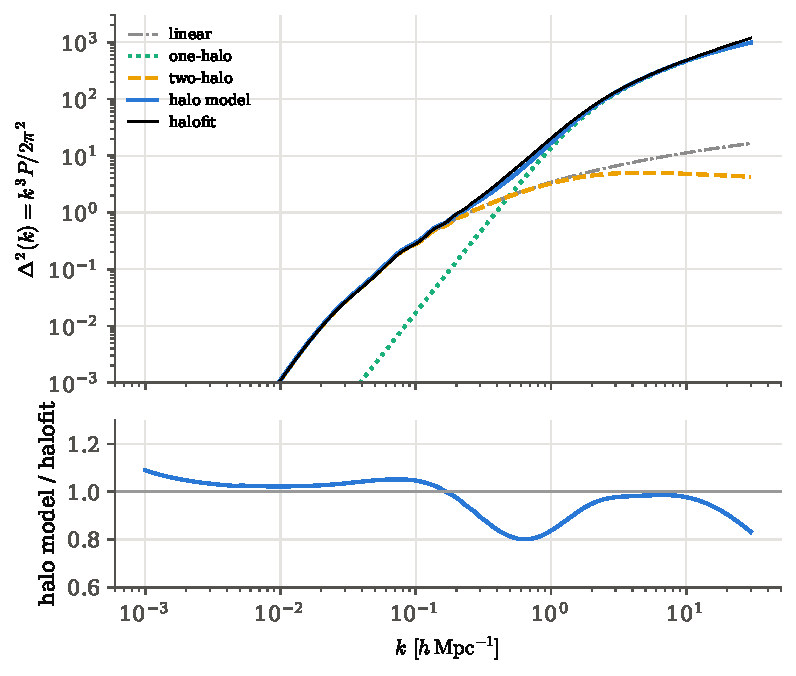
\includegraphics[width=0.8\linewidth]{figures/ch11/halo_model_pk.pdf}
\caption{The matter power spectrum at $z=0$ as $\Delta^2(k)=k^3P/2\pi^2$, the
contribution of each logarithmic interval of $k$ to the variance. The two-halo
term (dashed) follows linear theory (dash-dotted) and is cut off when $k$ resolves
the haloes; the one-halo term (dotted) rises as $k^3$ and takes over beyond
$k\approx\HmKeq\,h\,\mathrm{Mpc}^{-1}$. Their sum (blue) is compared with
halofit (black). Lower panel: the ratio of the two.}
\label{11b:fig:hm-pk}
\end{figure}

\paragraph{Side by side with halofit.}
\Cref{11b:fig:hm-pk} shows the result. The two terms are equal at
$k=\HmKeq\,h\,\mathrm{Mpc}^{-1}$. The ratio of the halo model to halofit is
$\HmRatioPtZeroOne$ at $k=0.01$, $\HmRatioPtOne$ at $0.1$, $\HmRatioPtThree$ at
$0.3$, $\HmRatioOne$ at $1$, $\HmRatioThree$ at $3$ and $\HmRatioTen$ at
$10\,h\,\mathrm{Mpc}^{-1}$. Between $k=0.05$ and $10$ the worst point is
$\HmRatioWorst$ at $k=\HmKworst\,h\,\mathrm{Mpc}^{-1}$. A handful of numbers
about haloes ($a$ and $p$ of the mass function, the amplitude and slope of the
concentration relation, the halo edge and $\delta_c$), each fixed by simulated or
spherical-collapse haloes and none adjusted to the power spectrum, reproduce a fit to simulations to within $20\%$ over three
decades in $k$, and to about $2\%$ between $k=3$ and $10\,h\,\mathrm{Mpc}^{-1}$.

\paragraph{Which haloes make the small-scale power?}
At $k=1\,h\,\mathrm{Mpc}^{-1}$ the one-halo term dominates, and the script
measures how it is shared among masses: $10\%$ of it comes from haloes below
$\HmMlo\times10^{13}\,h^{-1}M_\odot$ and $10\%$ from haloes above
$\HmMhi\times10^{13}$. The non-linear power on the scale of a few megaparsecs is
the internal structure of groups and clusters. That is why it is sensitive to
$\sigma_8$ and to everything that changes the cluster abundance, and why baryonic
processes inside clusters (gas blown out by active nuclei) change it measurably.

\paragraph{Where the halo model fails, and why.}
Each of the three disagreements traces back to one of the inputs.
\begin{itemize}[itemsep=2pt]
  \item \emph{The largest scales.} The one-halo term tends to a constant. Real
        matter has no such term: halo formation moves mass around locally and
        conserves it, and a local rearrangement of mass cannot create power
        that stays constant as $k\to0$ (it must vanish as $k^4$). The model's
        white noise adds $2\%$ at $k=0.01\,h\,\mathrm{Mpc}^{-1}$, more at smaller
        $k$ (\cref{11b:fig:hm-pk}, lower panel). The cause is (K1): the matter
        that went into a halo came from a surrounding region that is now
        underdense, and the model forgets the hole
        \srcref{CooraySheth2002}{\S4.4}.
  \item \emph{The transition, $k\approx0.3$--$1\,h\,\mathrm{Mpc}^{-1}$.} Here the
        model is up to $20\%$ low. The two-halo term uses linear $P$ and linear bias
        (K3), with no halo exclusion and no quasi-linear growth of the field
        between haloes, and the one-halo term only counts the matter inside
        $r_{\mathrm{vir}}$, not the infalling matter around it. Neither term
        is accurate where both are comparable. Research versions repair this region
        with fitted extra parameters \cite{Mead2015}.
  \item \emph{The smallest scales.} At $k\gtrsim3$ the answer depends on the
        concentration and on where the halo is cut. Keeping \eqref{11b:eq:conc}
        but cutting haloes at $200\bar\rho$ instead of $\HmDvir\bar\rho$ changes the
        ratio at $k=10$ from $\HmRatioTen$ to $\HmRatioTenTwoHundred$. The
        concentration relation is calibrated together with a halo definition,
        and only the pair is meaningful \srcref{CooraySheth2002}{\S5.4}.
\end{itemize}
The halo model is therefore a physical interpretation of the non-linear spectrum
accurate at the $10$--$20\%$ level, and a precise tool only after calibration.
Its value is that every piece has a meaning that can be changed on purpose:
massive neutrinos change $\sigma(M)$, baryons change $u(k\given M)$, modified gravity
changes $\delta_c$, and the model says which scales respond.

\subsection{Galaxies in haloes}
\label{11b:sec:hod}

Galaxies are not mass. Their correlation function is close to a power law,
$\xi_{gg}\propto r^{-\gamma}$ with $\gamma\approx1.8$, over two decades in
separation, while the matter correlation function is not a power law at all
\srcref{CooraySheth2002}{\S6}. Why should galaxies obey so simple a law when the
matter does not? In the halo model the answer comes from one more ingredient. Every
galaxy lives in a halo, so the galaxy field is the halo field reweighted by the
number of galaxies each halo hosts:
\begin{quote}
\emph{If a halo of mass $M$ hosts on average $\langle N\given M\rangle$ galaxies,
arranged in a known way, what are the galaxy power spectrum and correlation
function?}
\end{quote}

\paragraph{The occupation.}
A halo either has a galaxy at its centre or not; a central galaxy appears once the
halo is massive enough to cool gas and form stars. Further galaxies, the
satellites, orbit inside large haloes, distributed like the dark matter. A
standard form \cite{Zheng2005} is
\begin{equation}
  \langle N_c\given M\rangle=\frac12\Bigl[1+\operatorname{erf}
    \Bigl(\frac{\log_{10}M-\log_{10}M_{\min}}{\sigma_{\log M}}\Bigr)\Bigr],
  \qquad
  \langle N_s\given M\rangle=\langle N_c\given M\rangle\,
     \Bigl(\frac{M-M_0}{M_1}\Bigr)^{\alpha},
  \label{11b:eq:hod}
\end{equation}
the \newterm{halo occupation distribution} (HOD). The central count is a Bernoulli
variable (zero or one) with a smooth step in $\log M$; given a central, the number
of satellites is Poisson with mean $\lambda(M)=[(M-M_0)/M_1]^\alpha$, and there are
no satellites without a central. We take illustrative values,
$\log_{10}M_{\min}=\HodLMmin$, $\sigma_{\log M}=\HodSig$,
$\log_{10}M_0=\HodLMzero$, $\log_{10}M_1=\HodLMone$ and $\alpha=\HodAlpha$ (masses
in $h^{-1}M_\odot$), roughly those of luminous galaxies
(\cref{11b:fig:hod}, left).

\paragraph{The pairs inside one halo.}
The one-halo term of the matter came from pairs of mass elements in one halo,
weighted by $M^2$. For galaxies it comes from pairs of distinct galaxies in one
halo, so we need the mean number of ordered pairs, $\langle N(N-1)\given M\rangle$.
Write $N=C+S$ with $C\in\{0,1\}$ the central and $S$ the satellites:
\begin{align}
  \langle N(N-1)\given M\rangle
  &\eqby{1}\langle N_c\rangle\,\E\bigl[(1+S)S\given C=1\bigr]
   \eqby{2}\langle N_c\rangle\,\bigl(\lambda+\lambda+\lambda^2\bigr)
   \eqby{3}2\langle N_s\rangle+\langle N_c\rangle\lambda^2 .
  \label{11b:eq:hod-pairs}
\end{align}
\begin{explain}
  \item Without a central there are no galaxies and no pairs; with one,
        $N=1+S$, and this happens with probability $\langle N_c\rangle$.
  \item $\E[S]=\lambda$ and $\E[S^2]=\lambda+\lambda^2$ for a Poisson
        variable (\cref{ch:02}).
  \item $\langle N_s\rangle=\langle N_c\rangle\lambda$.
\end{explain}
The two terms are different kinds of pair. $2\langle N_s\rangle$ counts the
ordered pairs of the central with each satellite: one member sits at the centre
and the other is displaced by the profile, so in Fourier space such a pair carries
one factor $u(k\given M)$. $\langle N_c\rangle\lambda^2$ counts the ordered pairs
of two satellites, both displaced independently, which carry $u^2$
\srcref{CooraySheth2002}{pp.~65--66}. A Monte Carlo of $2\times10^6$ haloes of
$10^{14}\,h^{-1}M_\odot$ ($\langle N_c\rangle=\HodNcFourteen$,
$\lambda=\HodLamFourteen$) gives $\langle N(N-1)\rangle=\HodPairsMC\pm\HodPairsSE$
against $\HodPairsTh$ from \eqref{11b:eq:hod-pairs}.

\paragraph{The galaxy power spectrum.}
Replacing the mass weights $M/\bar\rho$ of \eqref{11b:eq:hm-derive} by galaxy
counts divided by the mean galaxy density
$\bar n_g=\int\dd M\,n(M)\langle N\given M\rangle$, and the self-pairs by the
pair counts just derived, gives
\begin{align}
  P_{gg}^{1h}(k)&=\frac{1}{\bar n_g^2}\int\dd M\,n(M)\,
     \bigl[2\langle N_s\given M\rangle\,u(k\given M)
     +\langle N_c\given M\rangle\lambda^2(M)\,u^2(k\given M)\bigr],\nonumber\\
  P_{gg}^{2h}(k)&=P_{\mathrm{lin}}(k)\Bigl[\frac{1}{\bar n_g}\int\dd M\,n(M)\,b(M)\,
     \bigl(\langle N_c\given M\rangle+\langle N_s\given M\rangle\,u(k\given M)\bigr)
     \Bigr]^2,
  \label{11b:eq:pgg}
\end{align}
\srcref{CooraySheth2002}{eqs.~(128)--(129)}. The pair of a galaxy with itself,
which we excluded, is the Poisson shot noise $1/\bar n_g$ of
\eqref{11a:eq:shot}, added on top when a catalogue is analysed. At small $k$ the
two-halo bracket becomes the \newterm{galaxy bias}
$b_g=\bar n_g^{-1}\int\dd M\,n\,b\,\langle N\given M\rangle$, the number-weighted
mean bias of the host haloes, so $P_{gg}\to b_g^2P_{\mathrm{lin}}$
\srcref{CooraySheth2002}{eqs.~(130)--(131)}.

\paragraph{Example: what the illustrative HOD predicts.}
The script gives $\bar n_g=\HodNbar\,h^3\mathrm{Mpc}^{-3}$, a satellite fraction of
$\HodFsat$, and $b_g=\HodBias$. The mean host mass, weighted by galaxy number, is
$\HodMeff\times10^{13}\,h^{-1}M_\odot$. The one-halo term tends to
$\HodOneHaloConst\,(h^{-1}\mathrm{Mpc})^3$ at small $k$, on top of the Poisson shot
noise $1/\bar n_g=\HodShot$ of the catalogue itself: galaxies sharing a halo add
pairs that a Poisson sample of a smooth field would not have, and this extra white
noise is about half the size of the Poisson term. This is the excess over the input (G2) of
\cref{11a:sec:cox-inputs}, ``no memory between places'', which holds between haloes
but not inside one. The correlation function, the Fourier transform of $P_{gg}$,
is close to a power law with $\gamma=\HodGamma$ and correlation length
$r_0=\HodRzero\,h^{-1}$Mpc between $0.2$ and $10\,h^{-1}$Mpc
(\cref{11b:fig:hod}, right), while the matter curve bends.

\begin{figure}[htbp]
\centering
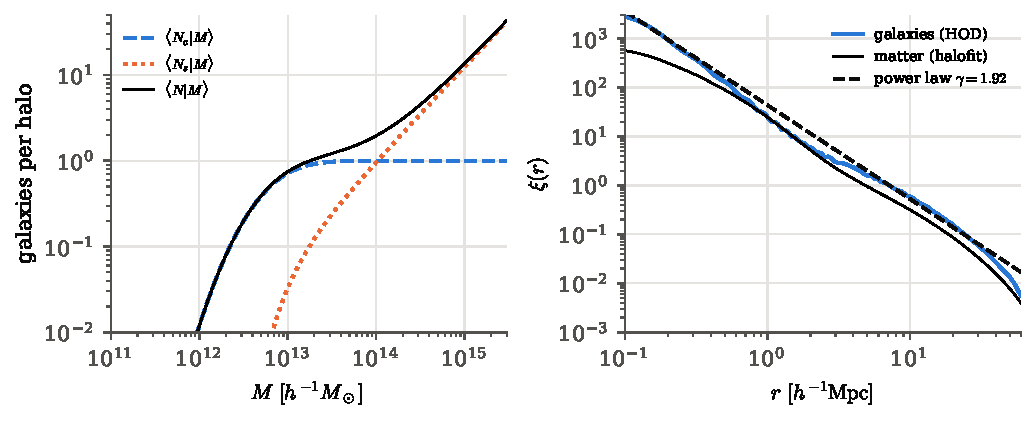
\includegraphics[width=\linewidth]{figures/ch11/hod_pk.pdf}
\caption{Left: the illustrative occupation \eqref{11b:eq:hod}: centrals
(dashed) switch on near $10^{13}\,h^{-1}M_\odot$, satellites (dotted) grow
almost in proportion to the halo mass. Right: the galaxy correlation function
from \eqref{11b:eq:pgg} (blue) against the matter correlation function from
halofit (black) and a power law (dashed). The galaxy curve is steeper than the
matter on small scales, where it is all one-halo pairs, and joins the scaled
matter curve on large scales.}
\label{11b:fig:hod}
\end{figure}

\paragraph{Why a power law?}
Below about $1\,h^{-1}$Mpc almost all pairs of galaxies sit in the same halo, and
the one-halo term, steep because it comes from the inner profiles of massive
haloes, sets $\xi_{gg}$. Above a few megaparsecs, pairs sit in different haloes and
$\xi_{gg}\approx b_g^2\xi_{\mathrm{lin}}$. Where the two hand over, the one-halo
term is falling and the two-halo term is flattening, and for galaxies whose
occupation is concentrated in massive haloes they happen to join smoothly. Change
the occupation and the slope changes. The power law is not a law; it is a
coincidence of two terms, and the HOD parameters are what a galaxy clustering
measurement on small scales actually constrains
\srcref{CooraySheth2002}{p.~66}.
\section{Voids}
\label{11b:sec:voids}

A redshift survey of the nearby Universe shows galaxies arranged in walls and
filaments around nearly empty regions tens of megaparsecs across. Bond, Kofman and
Pogosyan called the arrangement the \newterm{cosmic web} and showed that it is
already present, in embryonic form, in the initial Gaussian field: gravity only
sharpens the image \cite{BondKofmanPogosyan1996}. Clusters sit at the nodes, the
filaments join them, and the space in between, most of the volume, belongs to the
voids \cite{Wilding2021}. In \cref{11b:sec:same} the voids were where the
Zel'dovich universe and its phase-scrambled twin differed most. To use them as data
we need three things, which we take in turn:
\begin{enumerate}[label=(\arabic*),itemsep=1pt]
  \item \emph{What exactly counts as a void?} A rule that a computer can apply to
        a catalogue or a simulated field.
  \item \emph{How many voids of each size should a universe contain?} The
        prediction that turns a void count into a likelihood.
  \item \emph{What do voids look like on average, and what can their shape
        measure?} This is the subject of \cref{11b:sec:void-profiles}.
\end{enumerate}

\subsection{How an empty region evolves}
\label{11b:sec:void-evolution}

Start with the simplest void, a uniform spherical region of linear contrast
$\delta_{\mathrm{lin}}<0$ (extrapolated to today) in an Einstein--de Sitter
background. It is the spherical-collapse problem of \cref{11b:sec:hmf-inputs} run
backwards: the region expands faster than its surroundings and empties. The exact
solution is again taken from cosmology. For an underdense sphere of initial
comoving radius $R_0$ and linear contrast $\delta_0$ today, its comoving radius
$R$ and the redshift are given, in terms of a parameter $\theta$, by
\srcref{CooraySheth2002}{eq.~(50)}
\begin{equation}
  \frac{R}{R_0}=\frac{(1+z)}{(5/3)|\delta_0|}\,\frac{\cosh\theta-1}{2},
  \qquad
  \frac{1}{1+z}=\Bigl(\frac34\Bigr)^{2/3}\frac{(\sinh\theta-\theta)^{2/3}}{(5/3)|\delta_0|}.
  \label{11b:eq:void-param}
\end{equation}
\emph{What are the actual and the linear contrast at a given $\theta$?} The mass
inside the sphere is fixed, so its actual mean contrast is
$1+\Delta=(R_0/R)^3$; its linear contrast at that time is $\delta_0$ times the
growth factor, which in Einstein--de Sitter is $1/(1+z)$. Then
\begin{align}
  \delta_{\mathrm{lin}}
  &\eqby{1}\frac{\delta_0}{1+z}
   \eqby{2}-\frac35\Bigl(\frac34\Bigr)^{2/3}(\sinh\theta-\theta)^{2/3},\nonumber\\
  1+\Delta
  &\eqby{3}\Bigl[\frac{2\,(5/3)|\delta_0|}{(1+z)(\cosh\theta-1)}\Bigr]^3
   \eqby{4}\Bigl[2\Bigl(\frac34\Bigr)^{2/3}
     \frac{(\sinh\theta-\theta)^{2/3}}{\cosh\theta-1}\Bigr]^3
   =\frac92\,\frac{(\sinh\theta-\theta)^2}{(\cosh\theta-1)^3}.
  \label{11b:eq:void-curve}
\end{align}
\begin{explain}
  \item Linear growth in Einstein--de Sitter is $D\propto a=1/(1+z)$, normalised
        so that $D=1$ today.
  \item Insert $1/(1+z)$ from \eqref{11b:eq:void-param}, with $\delta_0=-|\delta_0|$;
        the $|\delta_0|$ cancels.
  \item $1+\Delta=(R_0/R)^3$, with $R/R_0$ from \eqref{11b:eq:void-param}.
  \item Again insert $1/(1+z)$; the $|\delta_0|$ cancels, and
        $8\,(3/4)^2=9/2$.
\end{explain}
\Cref{11b:fig:void-evolution} plots the curve. Two numbers on it define voids in
practice. First, the conventional threshold $\Delta=\VdThr$ is reached at
$\delta_{\mathrm{lin}}=\VdDv$. Second, a void whose density decreases outwards does
not stay smooth: its inner shells, more underdense, expand faster than the outer
ones and catch up with them, piling matter into a ridge at the edge. For a top hat
this \emph{shell crossing} happens at $\theta\approx3.53$, where
$\delta_{\mathrm{lin}}=\VdDvSc$ and $\Delta=\VdDnlSc$
\srcref{ShethvdWeygaert2004}{\S3.1}. The void has then become a distinct object
with a wall, the counterpart of collapse for a halo, and the threshold
\begin{equation}
  \delta_v=-2.81
  \label{11b:eq:deltav}
\end{equation}
plays the role of $\delta_c$. That is why void finders look for regions with
$\Delta\approx-0.8$. Since the mass inside is fixed, a void with $\Delta=-0.8$ is
larger than the Lagrangian region it came from by
\begin{equation}
  \frac{R}{R_L}=(1+\Delta)^{-1/3}=0.2^{-1/3}=\VdExpand ,
  \label{11b:eq:void-expand}
\end{equation}
\srcref{ShethvdWeygaert2004}{eq.~(7)}.

\paragraph{Example: the same void in the Zel'dovich approximation.}
Our simulated voids live in a Zel'dovich box, whose dynamics differ from the exact
spherical solution. For a uniform sphere of linear contrast $\delta_{\mathrm{lin}}$,
the Zel'dovich displacement is radial and, from $\nabla\cdot\bm\Psi=-\delta_{\mathrm{lin}}$
(\cref{11a:sec:rsd-python}), equal to $\bm\Psi=-\tfrac13\delta_{\mathrm{lin}}\,\bm q$,
because $\nabla\cdot\bm q=3$. A shell starting at $q$ moves to
$r=q(1-\delta_{\mathrm{lin}}/3)$, so
\begin{align}
  1+\Delta_{\mathrm{ZA}}
  &\eqby{1}\Bigl(\frac qr\Bigr)^3
   =\Bigl(1-\frac{\delta_{\mathrm{lin}}}{3}\Bigr)^{-3},
  \qquad
  \Delta_{\mathrm{ZA}}=-0.8
  \;\eqby{2}\;\delta_{\mathrm{lin}}=-3\,(5^{1/3}-1)=\VdDvZA .
  \label{11b:eq:za-void}
\end{align}
\begin{explain}
  \item Mass conservation inside the shell, as for the exact solution.
  \item Solve $(1-\delta/3)^{-3}=0.2$: $1-\delta/3=5^{1/3}$.
\end{explain}
The same formula with $\delta_{\mathrm{lin}}>0$ makes an overdense sphere collapse
to a point at $\delta_{\mathrm{lin}}=\VdDcZA$, in place of $\delta_c=1.686$. A
Zel'dovich void empties too fast (it keeps its initial velocities, while real
gravity decelerates the outflow), so it reaches $\Delta=-0.8$ at a smaller
$|\delta_{\mathrm{lin}}|$. These thresholds will matter when we compare the counted
voids with a prediction.

\begin{figure}[htbp]
\centering
\begin{tikzpicture}
\begin{axis}[width=10cm,height=6cm,xmin=-4,xmax=0,ymin=0,ymax=1.05,
  xlabel={linear contrast today, $\delta_{\mathrm{lin}}$},
  ylabel={$1+\Delta=\rho/\bar\rho$},
  every axis label/.style={font=\small},tick label style={font=\small},
  legend cell align=left,legend style={font=\scriptsize,at={(0.03,0.97)},anchor=north west,draw=none,fill=none}]
  \addplot[form,thick,domain=0.3:4.2,samples=200,variable=\t]
     ({-0.6*0.75^(2/3)*(sinh(\t)-\t)^(2/3)},{4.5*(sinh(\t)-\t)^2/(cosh(\t)-1)^3});
  \addlegendentry{spherical void, exact}
  \addplot[fibre,thick,dashed,domain=-4:0,samples=100] {(1-x/3)^(-3)};
  \addlegendentry{Zel'dovich}
  \addplot[faint,dotted,thick,domain=-1:0] {1+x};
  \addlegendentry{linear, $1+\delta_{\mathrm{lin}}$}
  \addplot[bdryred,dashed,domain=-4:0] {0.2};
  \node[lbl,bdryred,anchor=north east] at (axis cs:-0.05,0.19) {$\Delta=-0.8$};
  \draw[faint] (axis cs:-2.781,0) -- (axis cs:-2.781,0.2);
  \draw[faint] (axis cs:-2.13,0) -- (axis cs:-2.13,0.2);
  \node[lbl,anchor=south east,formblue] at (axis cs:-2.83,0.23) {$\VdDv$};
  \node[lbl,anchor=north west,fibreorange] at (axis cs:-2.08,0.15) {$\VdDvZA$};
\end{axis}
\end{tikzpicture}
\caption{The mean density inside a spherical void against its linear contrast.
Linear theory (dotted) reaches zero density at $\delta_{\mathrm{lin}}=-1$ and
then goes negative; the exact solution (blue) empties smoothly and reaches
$20\%$ of the mean density at $\delta_{\mathrm{lin}}=\VdDv$; the Zel'dovich
approximation (orange, dashed) gets there earlier, at $\VdDvZA$.}
\label{11b:fig:void-evolution}
\end{figure}

\subsection{Finding voids}
\label{11b:sec:voids-finder}

There is no unique definition of a void, only rules, and different rules find
different objects. Two families are in use.

\begin{workdef}[void (two operational definitions)]
\emph{Spherical underdensity:} a sphere about a local density minimum, grown until
the mean contrast inside it, $\Delta(<R)$, first rises to a threshold, usually
$-0.8$; overlapping spheres are pruned, largest first. The void radius is $R$.
\emph{Watershed:} treat the density as a landscape and flood it from every local
minimum; a void is the basin of one minimum, ending on the density ridges that
separate it from its neighbours \cite{Platen2007,Neyrinck2008}. Its effective
radius is that of the sphere of equal volume, $R=(3V/4\pi)^{1/3}$.
\end{workdef}

The spherical rule ties directly to the theory of
\cref{11b:sec:void-evolution}: it finds exactly the regions that have reached
$\Delta=-0.8$. The watershed rule needs no threshold and follows the real shapes of
voids; it is what most research catalogues use, including the ZOBOV code behind the
profiles of \cref{11b:sec:hamaus}.

\pyfile[firstline=226,lastline=268]{code/ch11/lib_web.py}{The spherical void
finder.}

\noindent
The finder smooths the gridded density with a Gaussian of one cell and takes as
seeds the cells that are lower than all 26 neighbours, with $\delta<-0.5$. For every
trial radius it computes the mean density in a sphere about \emph{every} cell at
once, by a Fourier-space convolution (\texttt{sphere\_average}); reading those maps
at the seeds gives $\Delta(<R)$ for every seed and every radius. The void radius
is where $\Delta(<R)$ first rises through the threshold, interpolated between trial
radii. Finally the voids are sorted by size and each is kept only if it does not
overlap a larger one already kept, with distances measured across the periodic
boundary.

\paragraph{Example: the voids of the Zel'dovich box.}
On the Zel'dovich universe of \cref{11b:sec:same} ($\SameL\,h^{-1}$Mpc,
$\SameN^3$ particles, cells of $3.1\,h^{-1}$Mpc) the finder returns
$\VdN$ voids larger than $\VdRmin\,h^{-1}$Mpc, with median radius
$\VdRmed\,h^{-1}$Mpc and largest $\VdRmax\,h^{-1}$Mpc. Together they fill only
$\VdVolFrac\%$ of the box. That is not a contradiction of ``voids fill most of the
volume'': the spherical rule keeps only the cores of the deepest regions, and the
non-overlap condition discards everything between them. The watershed rule, run on
the same field with the requirement that the basin floor be below $\delta=-0.8$,
gives $\VdNws$ basins of median effective radius $\VdRmedWs\,h^{-1}$Mpc, and the
basins tile the box. The two catalogues describe the same field and agree on
neither number nor size, which is why every void statistic must be predicted
with the same rule that measures it.

\subsection{How many voids: a walk between two barriers}
\label{11b:sec:svdw}

\emph{The obvious guess, and why it is wrong.} By symmetry with haloes, a point
should belong to a void of mass $M$ if its excursion-set walk first crosses
$\delta_v$, now from above, at $S=\sigma^2(M)$. That counts the
\emph{void-in-void} process correctly: a small void inside a larger one is part of
the larger one, exactly as a small halo inside a larger one is. But voids have a
second process with no counterpart for haloes \srcref{ShethvdWeygaert2004}{\S3.2}.
A small underdense region inside a large region that is collapsing is crushed
along with it. This is the \emph{void-in-cloud} process. In walk language: a walk
that crossed $\delta_c$ on some larger scale lies inside a halo, and any later
crossing of $\delta_v$ is not a void. So
\begin{quote}
\emph{a point belongs to a void of mass $M$ if its walk first crosses $\delta_v$
at $S=\sigma^2(M)$ without having crossed $\delta_c$ at any smaller $S$.}
\end{quote}
This is a random walk between two absorbing barriers, $\delta_v$ below and
$\delta_c$ above (\cref{11b:fig:void-barriers}, right).

\paragraph{What fraction of the mass ends up in voids?}
Let $p(x)$ be the probability that a walk now at height $x$, between the barriers,
reaches $\delta_v$ before $\delta_c$. Over a small step $\Delta S$ the walk moves to
$x+\epsilon$ with $\epsilon$ Gaussian of mean $0$ and variance $\Delta S$, and
from there the same question starts afresh, so
\begin{align}
  p(x)
  &\eqby{1}\E\bigl[p(x+\epsilon)\bigr]
   \eqby{2}p(x)+p'(x)\,\E[\epsilon]+\tfrac12p''(x)\,\E[\epsilon^2]+\dots
   \eqby{3}p(x)+\tfrac12p''(x)\,\Delta S+\dots\nonumber\\
  &\Longrightarrow\quad p''(x)=0
   \quad\eqby{4}\quad p(x)=\frac{\delta_c-x}{\delta_c-\delta_v}
   \quad\Longrightarrow\quad
   p(0)=\frac{\delta_c}{\delta_c+|\delta_v|}\equiv1-D .
  \label{11b:eq:ruin}
\end{align}
\begin{explain}
  \item Independent increments: after one step, the probability is that of
        a walk started from the new position, averaged over the step.
  \item Taylor expansion of $p$ about $x$.
  \item $\E[\epsilon]=0$, $\E[\epsilon^2]=\Delta S$; higher terms are of higher order
        in $\Delta S$.
  \item A function with zero second derivative is a straight line; the boundary
        conditions $p(\delta_v)=1$ and $p(\delta_c)=0$ fix it.
\end{explain}
This is the gambler's ruin of probability theory, and the result is
\srcref{ShethvdWeygaert2004}{eq.~(3)}, with the void-and-cloud parameter
$D=|\delta_v|/(\delta_c+|\delta_v|)$. For $\delta_v=\VdDv$ and $\delta_c=1.686$,
$1-D=\VdFracTh$: a bit over a third of the mass ends up in voids, the rest in
haloes. With $\delta_c=1.06$, the threshold for turnaround rather than full
collapse, it is $\VdFracThb$. The script \pyname{11_voids.py} runs $\VdNwalk$ walks
with both barriers, using \pyname{first_crossings} of \cref{11b:sec:hmf-mc} with
its lower barrier switched on, and finds $\VdFracMC$ and $\VdFracMCb$; the binomial
standard error is $0.0024$.

\paragraph{When do they cross?}
Now the distribution of the crossing scale. Let $p(\delta,S)$ be the density of
walks that are at height $\delta$ at time $S$ and have touched neither barrier. A
walk at $\delta$ after $S+\Delta S$ was at $\delta-\epsilon$ at $S$; the same
Taylor expansion as in \eqref{11b:eq:ruin}, now in $\delta$, gives the diffusion
equation $\partial p/\partial S=\frac12\partial^2p/\partial\delta^2$. Walks that
touch a barrier are removed, so $p=0$ at $\delta=\delta_v$ and at $\delta=\delta_c$;
all walks start at $0$, so $p(\delta,0)=\delta_D(\delta)$. Write $L=\delta_c-\delta_v$
for the gap between the barriers. Sine waves that vanish at both ends solve the
equation, each decaying at its own rate:
\begin{align}
  p(\delta,S)
  &\eqby{1}\sum_{j\ge1}A_j\sin\Bigl(\frac{j\pi(\delta-\delta_v)}{L}\Bigr)
     e^{-j^2\pi^2S/2L^2},
  \qquad
  A_j\eqby{2}\frac2L\sin\Bigl(\frac{j\pi|\delta_v|}{L}\Bigr)=\frac2L\sin(j\pi D),\nonumber\\
  \mathcal F_v(S)
  &\eqby{3}\frac12\,\frac{\partial p}{\partial\delta}\Big|_{\delta_v}
   \eqby{4}\sum_{j\ge1}\frac{j\pi}{L^2}\,\sin(j\pi D)\,e^{-j^2\pi^2S/2L^2}.
  \label{11b:eq:svdw-derive}
\end{align}
\begin{explain}
  \item Separation of variables: $\sin(j\pi(\delta-\delta_v)/L)$ vanishes at both
        barriers, and its second derivative is $-(j\pi/L)^2$ times itself, so the
        diffusion equation makes it decay as $e^{-j^2\pi^2S/2L^2}$.
  \item The coefficients of a delta function at $\delta=0$ in this sine series
        (Fourier sine series on an interval of length $L$); $0-\delta_v=|\delta_v|$
        and $|\delta_v|/L=D$.
  \item The rate at which walks leave through the lower barrier is the
        probability current there. For the diffusion equation with coefficient
        $\frac12$ the current is $-\frac12\partial p/\partial\delta$, which at the
        lower wall points downward with magnitude $\frac12\partial p/\partial\delta$.
  \item Differentiate the series term by term:
        $\partial_\delta\sin(j\pi(\delta-\delta_v)/L)=j\pi/L$ at $\delta=\delta_v$.
\end{explain}
Multiplying by $S$ and writing $1/L=D/|\delta_v|$ turns this into
\begin{equation}
  S\,\mathcal F_v(S)=\sum_{j\ge1}\frac{j^2\pi^2D^2}{\delta_v^2/S}\,
    \frac{\sin(j\pi D)}{j\pi}\,
    \exp\Bigl(-\frac{j^2\pi^2D^2}{2\,\delta_v^2/S}\Bigr),
  \label{11b:eq:svdw}
\end{equation}
which is \srcref{ShethvdWeygaert2004}{eq.~(1)}. The left panel of
\cref{11b:fig:void-barriers} compares it with the simulated walks, for both values
of $\delta_c$, and with the single-barrier answer ($\delta_c\to\infty$, $D\to0$,
the void-in-void process alone). The two-barrier curves are cut off at small
$\delta_v^2/S$, that is at small voids: those are the walks most likely to have
been inside a collapsing region first. At large voids the three agree, because a
large underdense region is almost never embedded in a larger collapsing one
\srcref{ShethvdWeygaert2004}{p.~11}.

\begin{figure}[htbp]
\centering
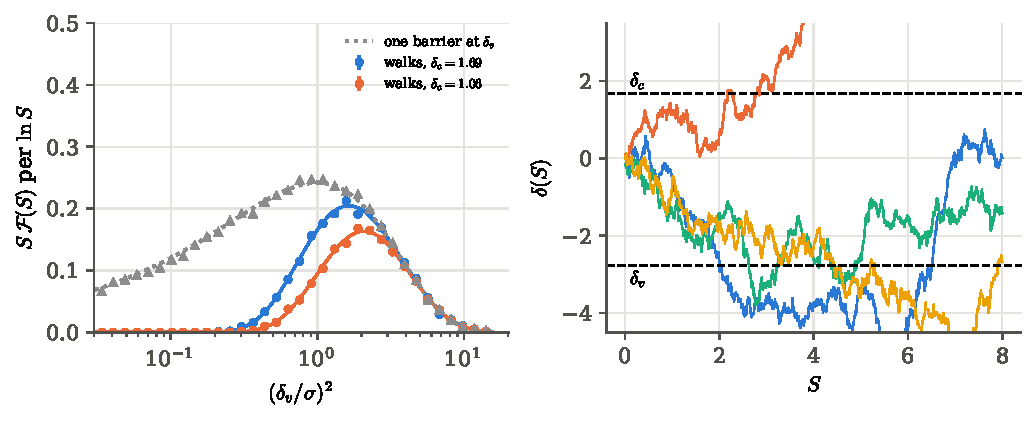
\includegraphics[width=\linewidth]{figures/ch11/void_barriers.pdf}
\caption{Left: the distribution of first down-crossings of $\delta_v$ that happen
before any crossing of $\delta_c$, per unit $\ln S$, from $\VdNwalk$ simulated
walks (points) and the series \eqref{11b:eq:svdw} (lines), for $\delta_c=1.686$
and $1.06$; grey: one barrier only. Right: four walks between the two barriers. A
walk that hits $\delta_c$ first belongs to a halo, and its later dips are voids
that have been crushed.}
\label{11b:fig:void-barriers}
\end{figure}

\paragraph{From walks to a size function.}
$S\mathcal F_v\,\dd\ln S$ is the fraction of mass in voids whose Lagrangian mass
has $\ln S$ in that interval. As for haloes, dividing by the mass of one void
counts them; a void of Lagrangian radius $R_L$ holds mass $\bar\rho V_L$, with
$V_L=\frac43\pi R_L^3$, and today has radius $R=\VdExpand\,R_L$. Hence the
number of voids per unit volume and unit $\ln R$,
\begin{equation}
  \frac{\dd n}{\dd\ln R}=\frac{S\mathcal F_v(S)}{V_L}\,
    \Bigl|\frac{\dd\ln S}{\dd\ln R_L}\Bigr|,
  \qquad S=\sigma^2(R_L),\quad R_L=R/\VdExpand ,
  \label{11b:eq:vsf}
\end{equation}
\srcref{ShethvdWeygaert2004}{eq.~(6)}. This model has a flaw that Sheth and van de
Weygaert point out themselves: every void is counted at the density of its
Lagrangian volume, then inflated by $\VdExpand^3=5$, so the total void volume can
exceed the volume of the Universe \srcref{ShethvdWeygaert2004}{p.~10}. Jennings,
Li and Hu \cite{Jennings2013} proposed instead that voids, as they expand, merge
rather than overlap, conserving the total volume in voids. That replaces $V_L$ by
the Eulerian volume $V=\frac43\pi R^3$ in \eqref{11b:eq:vsf}, the
``volume-conserving'' size function, a factor $\VdExpand^3$ lower.

\paragraph{Side by side with the Zel'dovich box.}
\Cref{11b:fig:void-sizes} compares the voids found in the box with both models,
computed with the CAMB $\sigma(R)$. With the thresholds of the dynamics that
actually made the box, $\delta_v=\VdDvZA$ and $\delta_c=\VdDcZA$ from
\eqref{11b:eq:za-void}, the counts lie between the two models: over radii
$9$--$19\,h^{-1}$Mpc Sheth--van de Weygaert is a factor $\VdSvdwRatio$ too high
(median ratio) and the volume-conserving model a factor $\VdVdnRatio$ too low. With
the exact spherical thresholds, $\delta_v=\VdDv$ and $\delta_c=1.686$, both
predictions drop steeply at large $R$; at $R=20\,h^{-1}$Mpc the Sheth--van de
Weygaert curve is $\VdGravRatioTwenty$ times lower than with the Zel'dovich
thresholds. The void abundance is exponentially sensitive to the threshold, for
the same reason as the cluster abundance: large voids are rare events in a Gaussian
field. That sensitivity is what makes the size function a probe of cosmology, and
what makes it fragile: a threshold that does not match the finder and the
dynamics shifts the prediction more than any change of cosmological parameters.
This is why research analyses calibrate the size function on simulations processed
with the same finder \cite{Contarini2023}.

\begin{figure}[htbp]
\centering
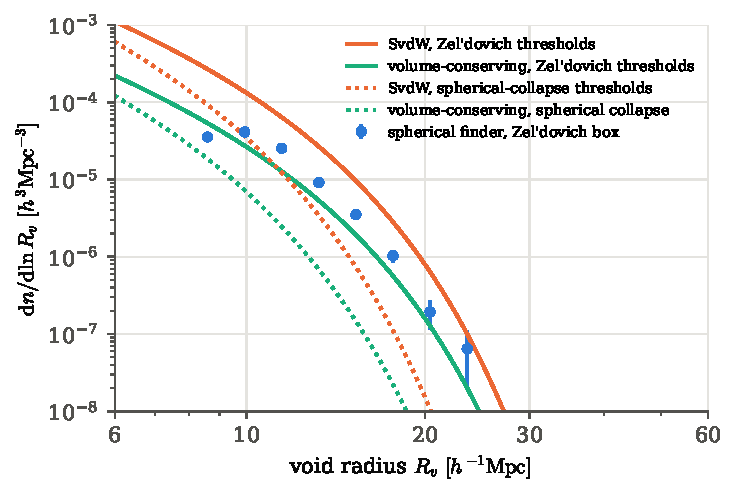
\includegraphics[width=0.8\linewidth]{figures/ch11/void_sizes.pdf}
\caption{The void size function of the Zel'dovich box (points, Poisson errors)
against the two-barrier excursion-set models: Sheth--van de Weygaert (orange) and
volume-conserving (green), with the thresholds of the Zel'dovich dynamics (solid)
and of exact spherical evolution (dotted). Over $9$--$19\,h^{-1}$Mpc the measured
counts lie between the two solid curves; the smallest bin, next to the finder's
minimum radius, falls below both.}
\label{11b:fig:void-sizes}
\end{figure}

\begin{keyidea}[Voids from two barriers]
A point is in a void of Lagrangian mass $M$ if its excursion-set walk first crosses
$\delta_v\approx-2.8$ at $S=\sigma^2(M)$ without first crossing $\delta_c$. The
mass fraction in voids is $\delta_c/(\delta_c+|\delta_v|)$, and the crossing
distribution is the sine series \eqref{11b:eq:svdw}. Converting it into numbers of
voids of each radius needs an assumption about how voids expand, and the result is
exponentially sensitive to the thresholds.
\end{keyidea}
\section{The average void: profile, outflow and shape}
\label{11b:sec:void-profiles}

A single void is an irregular hole with a lumpy wall. Average a few thousand of
them, each centred on its own centre and scaled by its own radius, and the
irregularities wash out. Nothing in a homogeneous, isotropic universe picks out a
direction, so the stacked void must be spherical, and its density and velocity
depend only on the distance from the centre in units of the void radius. That
average object is useful twice. Its radial profile records how matter has
streamed out of underdense regions, which depends on gravity and on the growth
rate. Its \emph{shape}, if we observe it with the wrong distances, is not
spherical, which turns the stack into a geometric ruler. We need the profile
first.

\subsection{Matter streams out of voids}
\label{11b:sec:void-velocity}

\emph{The question.} At distance $r$ from the centre of a spherical underdense
region, how fast does matter move away from it?

\emph{Linear theory.} The linear continuity equation,
$\dot\delta+\nabla\cdot\bm v/a=0$ (\eqref{11a:eq:theta}), relates the growth of
the density contrast to the divergence of the peculiar velocity $\bm v$. Integrate
it over a sphere of comoving radius $r$ about the centre, and let
$\Delta(r)=\frac{3}{r^3}\int_0^r\delta(r')\,r'^2\dd r'$ be the mean contrast inside:
\begin{align}
  \frac{4\pi r^3}{3}\,\dot\Delta
  &\eqby{1}\int_{|\bm x|<r}\dot\delta\,\dd^3x
   \eqby{2}-\frac1a\oint_{|\bm x|=r}\bm v\cdot\dd\bm A
   \eqby{3}-\frac{4\pi r^2}{a}\,v_r(r),\nonumber\\
  v_r(r)
  &\eqby{4}-\frac{a}{3}\,r\,\dot\Delta
   \eqby{5}-\frac13\,f\,aH\,r\,\Delta(r).
  \label{11b:eq:void-vlin}
\end{align}
\begin{explain}
  \item The integral of $\delta$ over the sphere is its volume times $\Delta$; the
        comoving sphere has fixed radius, so the time derivative acts on
        $\Delta$ alone.
  \item The continuity equation, and the divergence theorem.
  \item By spherical symmetry the radial velocity is the same all over the
        sphere.
  \item Solve for $v_r$.
  \item In linear theory every contrast grows as $D(t)$, so
        $\dot\Delta=(\dot D/D)\Delta=fH\Delta$ with $f=\dd\ln D/\dd\ln a$.
\end{explain}
At $z=0$, $a=1$ and this is \srcref{Hamaus2014}{eq.~(4)} with
$f\approx\Omega_m^{0.55}$. Inside a void $\Delta<0$, so $v_r>0$: matter flows out,
faster where the void is deeper and larger. With $r$ in $h^{-1}$Mpc and
$H_0=100\,h$\,km\,s$^{-1}$Mpc$^{-1}$, the factor $fH_0r$ is in km\,s$^{-1}$; for our
cosmology $f=\VdFzero$ at $z=0$.

\emph{Zel'dovich dynamics.} Linear theory is not trustworthy where
$\Delta\approx-0.8$. In the Zel'dovich approximation a particle moves as
$\bm x=\bm q+D\bm\Psi_0$, so its peculiar velocity is
$a\dot{\bm x}=a\dot D\bm\Psi_0=f\,aH\,\bm\Psi$. For a spherical void the
displacement is radial, and mass conservation fixes its size: the shell that is now
at $r$ started at $q$ with $q^3=(1+\Delta)r^3$, so
$\Psi_r=r-q=r[1-(1+\Delta)^{1/3}]$, and
\begin{equation}
  v_r^{\mathrm{ZA}}(r)=f\,aH\,r\,\bigl[1-(1+\Delta(r))^{1/3}\bigr],
  \label{11b:eq:void-vza}
\end{equation}
which reduces to \eqref{11b:eq:void-vlin} for small $\Delta$, since
$(1+\Delta)^{1/3}\approx1+\Delta/3$. For $\Delta=-0.8$ the bracket is
$1-0.2^{1/3}=0.42$, against $0.27$ in linear theory: the linear formula
underestimates the outflow from deep voids by a third.

\subsection{Reproducing Hamaus, Sutter and Wandelt}
\label{11b:sec:hamaus}

\paragraph{Their question.}
Halo profiles have a universal shape, NFW; do void profiles? In 2014 Hamaus,
Sutter and Wandelt \cite{Hamaus2014} asked for a simple formula that describes the
stacked density profile of voids of every size, out to several void radii,
including the overdense wall around the void, so that void statistics could be
modelled analytically rather than read off simulations.

\paragraph{Their setup.}
They used an $N$-body simulation of $2048^3$ dark matter particles in a box
$1\,h^{-1}$Gpc on a side with Planck cosmology, subsampled to
$\bar n=2\times10^{-2}\,h^3\mathrm{Mpc}^{-3}$, about the density of a galaxy
survey. Voids were found by the watershed code ZOBOV, keeping zones below
$\Delta=-0.8$; each void has an effective radius $r_v$ (the radius of the sphere
of the same volume), only voids larger than twice the mean particle separation were
used, and the profiles were measured in shells out to $3r_v$ and averaged in eight
bins of void radius \srcref{Hamaus2014}{p.~1}.

\paragraph{Their key equation.}
The formula they proposed is \srcref{Hamaus2014}{eq.~(2)}:
\begin{equation}
  \frac{\rho_v(r)}{\bar\rho}-1=\delta_{\mathrm{cen}}\,
  \frac{1-(r/r_s)^{\alpha}}{1+(r/r_v)^{\beta}} .
  \label{11b:eq:hamaus}
\end{equation}
It is an empirical fit, not a derived law, but every parameter can be read off from
the limits of the formula, and that is the derivation available. At $r\to0$ the
fraction is $1$, so $\delta_{\mathrm{cen}}$ is the central contrast. At $r=r_s$ the
numerator vanishes: $r_s$ is where the density crosses the mean, the inner edge of
the wall. For $r_s<r\lesssim r_v$ the numerator is negative, so the profile is
positive, the wall, with $\alpha$ setting how steeply it rises. For $r\gg r_v$ the
profile behaves as $-\delta_{\mathrm{cen}}(r/r_s)^\alpha(r_v/r)^\beta$, which goes to
zero only if $\beta>\alpha$; $\beta$ sets how fast the wall fades into the mean.
The total missing mass, $\int_0^\infty4\pi r^2\bar\rho\,\delta(r)\,\dd r$, converges
only if the integrand, $\propto r^{2+\alpha-\beta}$ at large $r$, falls faster than
$1/r$, that is if $\beta>\alpha+3$ \srcref{Hamaus2014}{eqs.~(7)--(8)}. Its sign
splits voids into \emph{overcompensated} ones, whose wall holds more than the
missing mass (small voids, embedded in collapsing regions), and
\emph{undercompensated} ones (large voids, embedded in larger underdense regions).
Hamaus et al.\ also found that $\alpha$ and $\beta$ follow $r_s/r_v$
\srcref{Hamaus2014}{eqs.~(10)--(11)}:
$\alpha\simeq-2(r_s/r_v-2)$, and
$\beta\simeq17.5\,r_s/r_v-6.5$ for $r_s/r_v<0.91$ and
$\beta\simeq-9.8\,r_s/r_v+18.4$ above. The velocity profile they compare with is
\eqref{11b:eq:void-vlin}, which we derived.

\begin{pitfall}[Two different ``$\delta_c$'']
Hamaus et al.\ call the central void contrast $\delta_c$. It has nothing to do
with the collapse threshold $\delta_c=1.686$ of \cref{11b:sec:hmf}. We write it
$\delta_{\mathrm{cen}}$.
\end{pitfall}

\paragraph{What we compute.}
\pyname{11_voids.py} runs the watershed finder of \cref{11b:sec:voids-finder} on
the Zel'dovich box, which gives $\VdNws$ voids, and for each void counts the
particles in $30$ shells out to $3R_v$ (using a $k$-d tree with periodic boundaries)
and divides by the expected count. It stacks the profiles in four bins of radius,
$10$--$13$, $13$--$16$, $16$--$20$ and $20$--$30\,h^{-1}$Mpc, with the standard
error of the mean as the error bar (never smaller than the Poisson error of the
stacked count). It fits \eqref{11b:eq:hamaus} to each stack with four free
parameters, by least squares, ignoring the innermost shells $r<0.15R_v$. For the
velocities, each particle's radial velocity is $fH_0\Psi_r$, and the stacked
mean is compared with \eqref{11b:eq:void-vlin} and \eqref{11b:eq:void-vza}, both
evaluated with the measured $\Delta(r)$ of the stack.

\paragraph{Side by side.}
\Cref{11b:fig:void-profiles} shows the stacks and the fits, and
\cref{11b:tab:hamaus} lists the parameters next to the values that the empirical relations for $\alpha(r_s/r_v)$ and
$\beta(r_s/r_v)$ quoted above would assign at our $r_s/R_v$.

\begin{table}[htbp]
\centering
\small
\begin{tabular}{ccccccccc}
\toprule
$\bar R_v$ & $N$ & $\delta_{\mathrm{cen}}$ & $r_s/R_v$ & $\alpha$ & $\beta$ &
$\chi^2/\text{dof}$ & $\alpha$ (H14) & $\beta$ (H14)\\
\midrule
$\VdRA$ & $\VdNA$ & $\VdDcA$ & $\VdRsA$ & $\VdAlA$ & $\VdBeA$\,(bound) & $\VdChiA/\VdDofA$ & $\VdAlHA$ & $\VdBeHA$\\
$\VdRB$ & $\VdNB$ & $\VdDcB$ & $\VdRsB$ & $\VdAlB$ & $\VdBeB$\,(bound) & $\VdChiB/\VdDofB$ & $\VdAlHB$ & $\VdBeHB$\\
$\VdRC$ & $\VdNC$ & $\VdDcC$ & $\VdRsC$ & $\VdAlC$ & $\VdBeC$ & $\VdChiC/\VdDofC$ & $\VdAlHC$ & $\VdBeHC$\\
$\VdRD$ & $\VdND$ & $\VdDcD$ & $\VdRsD$ & $\VdAlD$ & $\VdBeD$ & $\VdChiD/\VdDofD$ & $\VdAlHD$ & $\VdBeHD$\\
\bottomrule
\end{tabular}
\caption{Fits of \eqref{11b:eq:hamaus} to the stacked watershed voids of the
Zel'dovich box ($\bar R_v$ in $h^{-1}$Mpc). The last two columns are the values of
$\alpha$ and $\beta$ that the relations of \srcref{Hamaus2014}{eqs.~(10)--(11)}
give for the fitted $r_s/R_v$. ``Bound'': the fit ran into the upper limit
$\beta=25$ allowed in the fit.}
\label{11b:tab:hamaus}
\end{table}

For the two stacks of large voids the formula gets the shape roughly right. The
largest stack is fitted with $\chi^2=\VdChiD$ for $\VdDofD$ degrees of freedom, with
$r_s/R_v=\VdRsD$ close to the compensation value $0.91$ of
\srcref{Hamaus2014}{p.~3}, and $\alpha$ and $\beta$ near the
values Hamaus's relations assign. The next stack, with more voids and so smaller
errors, already has $\chi^2=\VdChiC$: close is not the same as right. The central contrasts, $-0.91$ to $-0.95$, are like
theirs ($-0.95$ for their voids of $11.7\,h^{-1}$Mpc, \srcref{Hamaus2014}{Fig.~3}). For the two stacks of small voids it fails: $\beta$ runs
to the edge of its allowed range and the $\chi^2$ is thousands. The reason is
visible in the left panel. Our small voids have almost no wall: the highest density
outside $0.8R_v$ is $\VdWallA$ for the smallest stack, against $\VdWallD$ for the
largest, and their density approaches the mean slowly from below out to $3R_v$.
Hamaus's small voids have the highest walls of all.

\paragraph{Why they differ.}
Two causes, both in our simulation rather than in the formula. First, the
Zel'dovich approximation has no gravity after the initial kick: particles that meet
in a wall do not stop there but stream through it, so walls, which in a real
universe are built by matter piling up and staying, are thin and short-lived. The
small overcompensated voids of an $N$-body simulation are surrounded by just such
walls, collapsing around them (the void-in-cloud process of \cref{11b:sec:svdw}).
Second, the watershed of a smoothed Zel'dovich field splits large underdense
regions into several basins, so many of our small ``voids'' are sub-basins of a
larger void, undercompensated by construction. Only large voids, whose walls
formed from large-scale linear modes that Zel'dovich treats well, look like the
$N$-body ones. The errors of the stacks are also small (thousands of voids, millions
of particles), so the $\chi^2$ detects any mismatch of shape.

\paragraph{The outflow.}
The right panel of \cref{11b:fig:void-profiles} shows the stacked radial
velocities. For the largest stack the peak outflow is $\VdVmaxD$\,km\,s$^{-1}$,
against $\VdVzamaxD$ from the spherical Zel'dovich formula \eqref{11b:eq:void-vza}
and $\VdVlinmaxD$ from linear theory \eqref{11b:eq:void-vlin}. The linear formula
is too low by about a third inside the void, close to the factor estimated after
\eqref{11b:eq:void-vza}. The Zel'dovich formula comes within a few per cent,
about as close as the few hundred voids of one stack allow. That agreement is
partly a consistency check, since the particle velocities in our box are
Zel'dovich velocities; it confirms that the stacked void behaves like a spherical
one.

\paragraph{The lesson.}
A fitting formula is universal only within the dynamics that produced it: our large
voids follow the Hamaus profile, our small ones do not, because a Zel'dovich
universe cannot build the walls that make small voids overcompensated.

\begin{figure}[htbp]
\centering
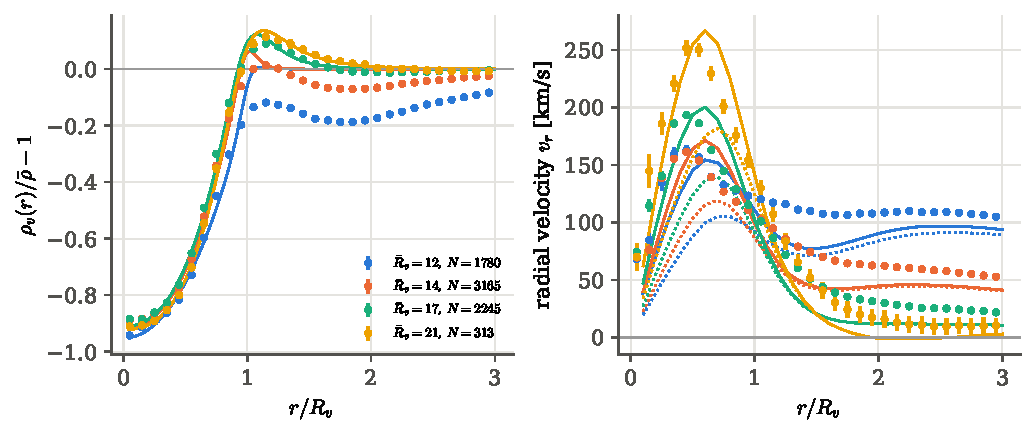
\includegraphics[width=\linewidth]{figures/ch11/void_profiles.pdf}
\caption{Stacked watershed voids of the Zel'dovich box in four bins of radius.
Left: density profiles (points) and fits of \eqref{11b:eq:hamaus} (lines); only the
larger voids have an overdense wall near $R_v$. Right: radial velocity profiles
(points) with the spherical Zel'dovich prediction (solid) and linear theory
(dotted), both from the measured enclosed contrast.}
\label{11b:fig:void-profiles}
\end{figure}

\subsection{Voids as standard spheres}
\label{11b:sec:void-ap}

\paragraph{The question.}
In a homogeneous, isotropic universe the stacked void is a sphere. A survey does not
measure distances; it measures angles and redshifts, and converts them with a
fiducial cosmology (\cref{11a:sec:alpha}). If the fiducial cosmology is wrong, does
the stacked void still look round? Lavaux and Wandelt \cite{LavauxWandelt2012}
proposed using exactly this, a test of sphericity first suggested by Alcock and
Paczy\'nski for any population of round objects.

\emph{The geometry.} Write $\alpha_\perp=D_M/D_M^{\mathrm{fid}}$ and
$\alpha_\parallel=D_H/D_H^{\mathrm{fid}}$ for the ratios of the true to the
fiducial transverse and radial distances, as in
\eqref{11a:eq:alpha-perp-par}. A sphere of true radius $R_0$ appears with
transverse radius $R_0/\alpha_\perp$ and radial radius $R_0/\alpha_\parallel$, so
its apparent axis ratio is
\begin{equation}
  q\equiv\frac{R_\parallel^{\mathrm{fid}}}{R_\perp^{\mathrm{fid}}}
  =\frac{\alpha_\perp}{\alpha_\parallel}
  =\frac{D_M/D_M^{\mathrm{fid}}}{D_H/D_H^{\mathrm{fid}}}
  =\frac{D_M(z)H(z)}{[D_M(z)H(z)]^{\mathrm{fid}}},
  \label{11b:eq:ap-q}
\end{equation}
using $D_H=c/H$. The size of the void depends on the unknown true radius, but the
ratio does not: a population of spheres measures the product $D_MH$ without any
ruler of known length \srcref{LavauxWandelt2012}{eqs.~(5)--(9)}. This is the
\newterm{Alcock--Paczy\'nski test}.

\emph{What curve do we fit?} A sphere of radius $R_0$ stretched by $q$ along the
line of sight has points $(r_\perp,r_\parallel)$ with
$r_\perp^2+(r_\parallel/q)^2=R_0^2$. In polar form, $r_\perp=r\sqrt{1-\mu^2}$ and
$r_\parallel=r\mu$, with $\mu$ the cosine of the angle to the line of sight:
\begin{equation}
  r^2\Bigl(1-\mu^2+\frac{\mu^2}{q^2}\Bigr)=R_0^2
  \quad\Longrightarrow\quad
  r(\mu)=\frac{R_0}{\sqrt{1-\mu^2\,(1-1/q^2)}} .
  \label{11b:eq:ellipse}
\end{equation}

\paragraph{The experiment.}
\pyname{12_void_ap.py} takes the $\ApNvoid$ spherical voids with
$10\le R_v<25\,h^{-1}$Mpc from \cref{11b:sec:voids-finder}, and stacks the particles
around them in bins of $r/R_v$ and $|\mu|$, with the box's $z$ axis as the line of
sight. In each of ten $\mu$ bins it finds the radius where the stacked density
rises through $\ApLevel$, and fits \eqref{11b:eq:ellipse} to those ten radii.
The error of $q$ comes from a \newterm{jackknife}, a resampling estimate in the
spirit of the bootstrap of \cref{3b:sec:bootstrap}: cut the box into
$G=\ApNjk$ sub-cubes and put each void in the group of the sub-cube that holds its
centre, repeat the whole measurement $G$ times leaving out one group at
a time to get $q_1,\dots,q_G$, and take
$\sigma_q^2=\frac{G-1}{G}\sum_g(q_g-\bar q)^2$. The factor $G-1$ compensates for
the leave-one-out values being much closer to each other than independent
measurements would be, since any two of them share $G-2$ of the $G$ groups.
The groups are regions of space, not voids picked at random, because
neighbouring voids sit in the same large-scale waves and are not independent;
leaving out a whole region removes those waves too. Even so, every region lies
in the same box, and the jackknife cannot see waves longer than the box. The
error is a rough one.

The script measures $q$ four times: in real space; with the line of sight
stretched by a true $q=\ApQtrue$, as a wrong fiducial cosmology would do; in
redshift space, moving each particle by its line-of-sight velocity, $s_z=z+f\Psi_z$
(\cref{11a:sec:rsd-map}); and with both.

\begin{figure}[htbp]
\centering
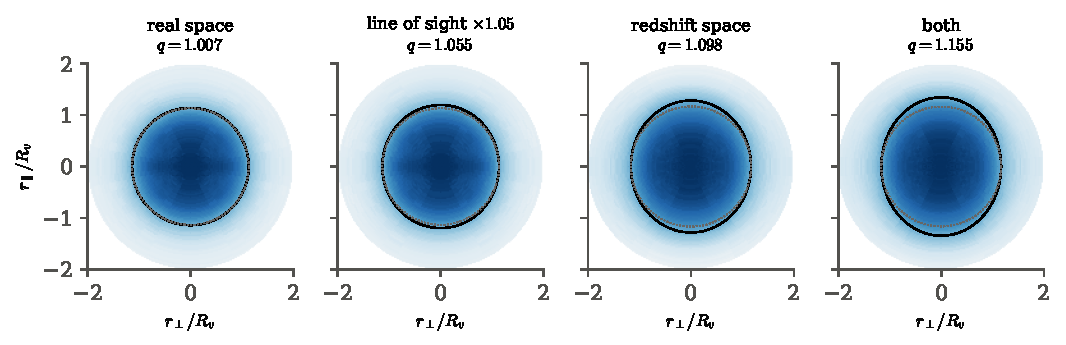
\includegraphics[width=\linewidth]{figures/ch11/void_ap.pdf}
\caption{The stacked void in the plane of the line of sight (vertical) and a
transverse direction, coloured by density (blue empty, red dense), with the fitted
ellipse (black) and a circle (dotted). From left to right: real space; real space
with distances along the line of sight stretched by $\ApQtrue$; redshift space;
both. Stretching and redshift-space outflow both elongate the stack.}
\label{11b:fig:void-ap}
\end{figure}

\paragraph{What it finds.}
In real space $q=\ApQreal\pm\ApQrealErr$: the stack is round, as isotropy demands.
With the stretched line of sight $q=\ApQap\pm\ApQapErr$, which recovers the input
$\ApQtrue$. About fifteen hundred voids in $0.2\,(h^{-1}\mathrm{Gpc})^3$ measure
the axis ratio to about $\ApQapPct\%$. But in redshift space, with the correct geometry,
$q=\ApQrsd\pm\ApQrsdErr$, and with both effects $q=\ApQboth\pm\ApQbothErr$, close to
the product $\ApQap\times\ApQrsd=\ApQprod$. The outflow of matter from voids
elongates them along the line of sight by more than the geometric signal we
inserted.

\paragraph{Why the outflow elongates the void.}
Redshift space moves every particle along the line of sight by $f\Psi_z$. Near a
spherical void the displacement is radial, $\bm\Psi=\Psi_r(r)\,\hat{\bm r}$, so
$\Psi_z=\Psi_r(r)\,z/r$. The density in redshift space is the real density divided
by the Jacobian of the map, $1+f\,\partial\Psi_z/\partial z$
(\cref{11a:sec:kaiser}), and
\begin{align}
  \frac{\partial\Psi_z}{\partial z}
  &\eqby{1}\Psi_r'(r)\,\frac{z}{r}\,\frac{\partial r}{\partial z}
   +\Psi_r(r)\Bigl(\frac1r-\frac{z}{r^2}\frac{\partial r}{\partial z}\Bigr)
   \eqby{2}\mu^2\,\Psi_r'(r)+(1-\mu^2)\,\frac{\Psi_r(r)}{r}.
  \label{11b:eq:void-jac}
\end{align}
\begin{explain}
  \item Product rule on $\Psi_r(r)\cdot z/r$.
  \item $\partial r/\partial z=z/r=\mu$.
\end{explain}
Along the line of sight ($\mu=1$) the shell at $r$ moves out by $f\Psi_r$ and its
density is divided by $1+f\Psi_r'$. Across it ($\mu=0$) nothing moves, but the
density is still divided by $1+f\Psi_r/r$, because the outflow stretches the line
of sight around every point. Both make the void look emptier, and so larger, but by
different amounts, so the void becomes elongated. Using the measured real-space
stack and the spherical Zel'dovich $\Psi_r$, the script predicts that the
$\ApLevel$ contour moves out by a factor $\ApParZA$ along the line of sight and
$\ApPerpZA$ across it (linear theory: $\ApParLin$ and $\ApPerpLin$), an axis ratio of
$\ApQcontZA$ (linear: $\ApQcontLin$), against the measured $\ApQrsd\pm\ApQrsdErr$.
The ratio is right. The two radii separately are both overpredicted by a few per
cent (measured: $\ApParMeas$ in the $\mu$ bin nearest the line of sight and
$\ApPerpMeas$ in the bin nearest the transverse direction), a common offset that
the spherical model does not capture and that cancels in the ratio.

\paragraph{Example: what the test would measure.}
At $z=\ApZ$, the mean redshift of the BOSS void sample, our fiducial flat
$\Lambda$CDM has $D_MH/c=\ApDMH$, and $\dd\ln(D_MH)/\dd\Omega_m=\ApDlnqDom$. An
error of $\ApQapErr$ on $q\approx\ApQtrue$ therefore corresponds to
$\sigma(\Omega_m)\approx\ApQapErr/(\ApQtrue\times\ApDlnqDom)=\ApSigOm$, for a stack
of the size of ours (as rough as the jackknife error it comes from), if the redshift-space elongation were known exactly. The BOSS
analysis of Hamaus et al.\ \cite{Hamaus2020} fitted the redshift-space distortion
($f/b$, the growth rate over the galaxy bias) and the geometry at the same time, and
found $D_MH/c=\ApDMHHam\pm\ApDMHHamErr$ at $z=0.51$ (they write $D_A$ for our
comoving $D_M$), with $f/b=0.540\pm0.091$ and, in flat $\Lambda$CDM,
$\Omega_m=0.312\pm0.020$.

\begin{keyidea}[Stacked voids as standard spheres]
The stacked void is spherical in true coordinates, so its axis ratio in survey
coordinates measures $D_M(z)H(z)$ relative to the fiducial value, with no ruler of
known length. The outflow from voids elongates the stack along the line of sight by
a comparable amount, so the geometry and the growth rate must be fitted together.
\end{keyidea}

\subsection{What voids are sensitive to}
\label{11b:sec:void-sensitivity}

Voids are the regions where the matter is thinnest, and that makes them respond to
physics that the dense regions hide \srcref{Pisani2019}{\S2}.
\begin{itemize}[itemsep=2pt]
  \item \emph{Dark energy.} A void is the part of the Universe where dark energy
        dominates first. Its expansion is set by gravity, which empties it, and by
        the cosmic expansion, which stretches it, so the size function depends on
        the dark-energy equation of state; and the Alcock--Paczy\'nski test above
        measures $D_MH$ directly. The BOSS void size function alone gives
        $w=-1.1\pm0.2$ \cite{Contarini2023}.
  \item \emph{Modified gravity.} Many alternatives to general relativity add a
        force that is screened in dense environments, so that solar-system tests
        are passed. Voids are where screening fails: the extra force makes them
        expand faster and empty further, which shows up in their size function and
        in the outflow measured by redshift-space distortions around them.
  \item \emph{Massive neutrinos.} Neutrinos stream freely over distances comparable
        to void sizes and do not follow the dark matter out of voids. Their share
        of the mass is therefore higher in voids than in dense regions, which
        changes how many voids form, how empty they become, and how they cluster.
\end{itemize}
Each of these is a change of the inputs of \cref{11b:sec:svdw} ($\sigma(R)$, the
thresholds, the expansion factor) or of the outflow \eqref{11b:eq:void-vlin}
(through $f$), which is why the excursion-set and velocity models are the
starting point of every void forecast.

\subsection{Voids and the topology of the field}
\label{11b:sec:void-topology}

Does the way the regions of a field are connected carry information that the
power spectrum does not expose? Topology is the tool made for that question, and
the cosmic web has an exact topological description, which \cref{ch:12} builds
from the beginning. Take the region where the density exceeds a threshold $t$, the
superlevel set $\{\delta>t\}$. Its Betti numbers count, in three dimensions, its
connected pieces ($\beta_0$), its independent tunnels ($\beta_1$) and the cavities
it encloses ($\beta_2$) (see the topology notes). A void, seen from the matter, is a
cavity: an empty region enclosed by walls. Voids are the $\beta_2$ features of the
cosmic web \cite{Pranav2017,Wilding2021}. Equivalently, a cavity of the superlevel
set is a separate connected piece of the complementary sublevel set
$\{\delta<t\}$, and connected pieces are what a computer counts most easily.

\pyname{11_voids.py} counts them in the Zel'dovich box, after smoothing by one cell
as for the watershed: the number of connected regions of $\{\delta_s<t\}$ (with the
periodic faces glued, by a union--find over the labels on opposite faces), and the
number of local minima below $t$, as $t$ rises from $-0.95$ to $0$
(\cref{11b:fig:void-topology}). Every region is born at a local minimum, so the
minima are the births. At $t=-0.8$ there are $\VdNcompEight$ regions and
$\VdNminEight$ minima: most minima are still separate voids. The number of regions
peaks at $\VdNcompMax$ near $t=\VdTcompMax$ and then falls while minima keep
appearing, because regions merge at saddle points of the density; by $t=-0.5$ there
are $\VdNcompFive$ regions for $\VdNminFive$ minima, and at $t=0$ only
$\VdNcompZero$. The underdense regions have joined into a network that runs through
the box. That the separate voids exist only below $\delta\approx-0.8$ is the same
threshold that came out of spherical evolution, and the one Wilding et al.\ find in
$N$-body simulations, below which voids are the only topological features of the
field \srcref{Wilding2021}{p.~10}.

\begin{figure}[htbp]
\centering
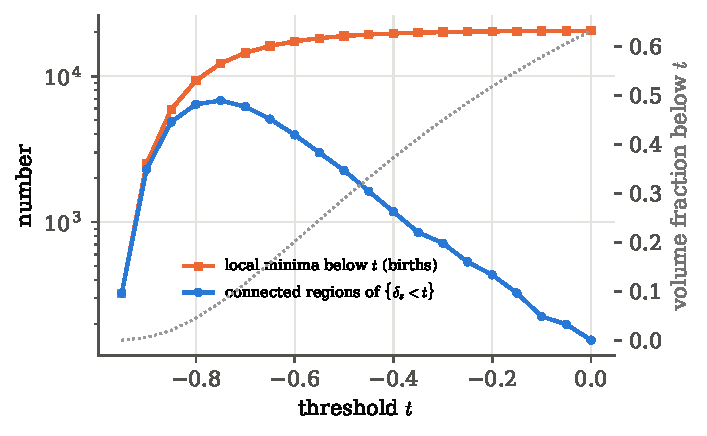
\includegraphics[width=0.72\linewidth]{figures/ch11/void_topology.pdf}
\caption{Underdense regions of the smoothed Zel'dovich field as the threshold $t$
rises: the number of separate connected regions of $\{\delta_s<t\}$ (blue), the
number of local minima below $t$ (orange), and the volume fraction below $t$
(dotted, right axis). Each region is born at a minimum; the gap between the curves
counts the mergers at saddles.}
\label{11b:fig:void-topology}
\end{figure}

The picture is the one that persistence formalises. Each underdense region is born
at the value of its minimum and dies when it merges with an older one at a saddle;
the pair (birth, death) is a point of a persistence diagram, and the watershed
basins of \cref{11b:sec:voids-finder} are the regions between those saddles. A
void finder is therefore a particular, hand-tuned reading of the $H_0$ persistence of
the sublevel sets. \Cref{ch:12} turns that reading into a statistic with a sampling
distribution and feeds it to the same likelihood machinery as $P(k)$.
\section{Haloes and voids in research}
\label{11b:sec:research}

Every measurement of haloes and voids we have made came from a script that runs
in seconds to minutes on a laptop. The research
versions keep the same ideas (first crossings, profiles, one- and two-halo terms,
two barriers, stacked spheres) and replace almost every ingredient by something
measured in large simulations.

\paragraph{Haloes.}
Research groups do not take the mass function from a formula. They run $N$-body
simulations of $10^9$--$10^{11}$ particles in boxes of a few $h^{-1}$Gpc, identify
haloes with a halo finder (linking particles closer than a fraction of the mean
separation, or growing spheres to a fixed overdensity, the same choice of edge that
mattered in \cref{11b:sec:hm-python}), and fit or emulate $\dd n/\dd\ln M$ and
$b(M)$ as functions of cosmology. The excursion set and the peak-background split
survive as the reason the fits are nearly universal in $\nu$ and as a check on
them. For cluster counts the hard part is not the mass function but the
mass: clusters are found by their galaxies, hot gas or lensing signal, and the
relation between that observable and $M$ is calibrated with weak lensing, which
is now the dominant uncertainty.

\paragraph{The non-linear power spectrum.}
The version of the halo model used in practice is HMcode \cite{Mead2015},
available in CAMB: the halo model of \cref{11b:sec:halomodel} with a handful of
extra parameters fitted to simulations, which smooth the transition region where
our version was $20\%$ low and remove the large-scale one-halo excess. Because each
parameter has a physical meaning, the same code models baryonic feedback by
changing the concentration and the inner profiles of haloes, which is how weak
lensing surveys marginalise over baryons. Halofit \cite{Takahashi2012}, which
we compared with, plays the same role without the physical parameters, and
emulators trained on suites of simulations are replacing both at the per-cent
level.

\paragraph{Galaxies.}
The halo occupation distribution of \cref{11b:sec:hod} is fitted to the measured
small-scale clustering of each galaxy sample, usually the projected correlation
function, with the HOD parameters as nuisance parameters. The fitted HOD is then
used to place galaxies in the haloes of $N$-body or approximate simulations, which
produces the thousands of mock catalogues from which the covariance matrices of
\cref{11a:sec:research} are estimated. So the halo model enters every survey
analysis, if only through its mocks.

\paragraph{Voids.}
Void catalogues are built from the galaxies of spectroscopic surveys (BOSS,
eBOSS, and now DESI, with Euclid to follow) with watershed codes descended from
ZOBOV \cite{Neyrinck2008}, run on the survey's light cone with its mask and
selection. Galaxies are sparse and biased, so the voids are defined by the
tracers, not by the matter, and their sizes depend on the tracer density; every
prediction is therefore calibrated on mock catalogues processed by the same
finder. The two leading analyses are the ones met above: the joint fit of the
redshift-space distortions and the Alcock--Paczy\'nski distortion of the stacked
void--galaxy cross-correlation \cite{Hamaus2020}, and the void size function with
a volume-conserving model extended by calibrated nuisance parameters
\cite{Contarini2023}.

\begin{inpractice}[Verification and research]
Our simulations played two roles. The random walks of
\cref{11b:sec:hmf-mc,11b:sec:svdw} \emph{verified} results we had derived
exactly: the factor of $2$, the Press--Schechter multiplicity, the gambler's-ruin
void fraction and the two-barrier series. The Zel'dovich box was used as a
stand-in for the \emph{research} instrument, the place where no closed form exists:
the void size function measured with a particular finder, the stacked profiles, the
redshift-space elongation of voids, the topology of the underdense regions. In
research that instrument is an $N$-body simulation with the survey's tracers,
mask and finder, and the analytic models are calibrated against it, never the other
way round.
\end{inpractice}

\subsection{What our shortcuts cost}
\label{11b:sec:research-nerfs}

\Cref{11b:tab:nerfs} lists each simplification, what research does instead, and
what it costs. As in \cref{11a:sec:research-nerfs}, some costs are only wider
error bars or a smaller range of scales; others leave a physical effect out, and
no amount of laptop time in the same model brings it back.

\begin{table}[htbp]
\centering
\small
\begin{tabular}{p{2.0cm}p{3.6cm}p{3.6cm}p{4.0cm}}
\hline
step & research & ours & what it costs \\
\hline
dynamics & $N$-body, $10^9$--$10^{11}$ particles, Gpc boxes &
Zel'dovich particles, $\SameN^3$ in $\SameL\,h^{-1}$Mpc &
no bound haloes, walls dissolve after shell crossing; small voids lack their walls
(Hamaus fit fails for $R_v\lesssim15\,h^{-1}$Mpc); void thresholds are the
Zel'dovich ones \\
haloes & found in simulations; mass function and bias fitted or emulated &
analytic only (Press--Schechter, Sheth--Tormen) &
abundance uncertain by tens of per cent at the extremes; no test of the
peak-background split on simulated haloes \\
first crossings & correlated steps (real-space filters), moving barriers &
sharp-$k$ walks; $\HmfNfield$ fields of $\HmfFieldN^3$ cells for the top hat &
the factor of $2$ is exact only for the sharp-$k$ filter; the top-hat result has no
closed form \\
non-linear $P(k)$ & HMcode or emulators, with baryons &
plain halo model, one concentration relation &
$\HmRatioWorst$ at $k=\HmKworst\,h\,\mathrm{Mpc}^{-1}$; white-noise excess on
large scales; no baryons \\
galaxies & HOD fitted to measured clustering; mocks &
illustrative HOD, no fit &
the power-law $\xi_{gg}$ is a demonstration, not a measurement \\
void tracers & sparse, biased galaxies on the light cone, survey mask &
all particles, periodic box, $z=0$ &
voids smaller and emptier than in a survey; no mask or edge effects \\
void finder & ZOBOV/VIDE on tracers; calibrated on mocks &
grid-based spherical and watershed finders, one-cell smoothing &
size function differs from the two analytic models by factors of about $2$--$3$ \\
geometry & joint fit of AP and RSD on the void--galaxy cross-correlation &
ellipse fitted to one contour; AP and RSD separately &
$\sigma_q\approx\ApQapErr$ only for known RSD; no joint posterior \\
covariance & thousands of mocks & jackknife over $\ApNjk$ sub-cubes of one box, Poisson errors &
error bars approximate; stacked-profile $\chi^2$ not a calibrated test \\
\hline
\end{tabular}
\caption{The steps of the halo and void analyses at research scale and in our
scripts, with the cost of each simplification.}
\label{11b:tab:nerfs}
\end{table}

The first row matters most. Almost everything that went wrong in our comparisons, the missing walls of small voids, the need for Zel'dovich
thresholds in the size function, the close but partly circular agreement of
the void outflow, comes from the Zel'dovich dynamics. A particle-mesh $N$-body code
in a $256^3$ box would run on the laptop in tens of minutes and would remove most of
it; the full research version runs $N$-body simulations with $10^{10}$ particles on
thousands of cores and identifies haloes and voids in hundreds of snapshots. What
the laptop versions do transfer is the mechanism: why the mass function has the
shape it has, where each part of the non-linear power spectrum comes from, why the
galaxy correlation function is close to a power law, and why voids measure both
geometry and growth.

\begin{recap}
\begin{itemize}[leftmargin=1.2em,itemsep=2pt]
  \item Two fields with the same $|\delta_{\bm k}|$ share $P(k)$, $\xi(r)$ and
        $\sigma_R$ but can differ in skewness, one-point distribution and voids;
        the difference lives in the phases and is carried by haloes and voids
        (\cref{11b:sec:same}).
  \item With a sharp-$k$ filter the smoothed linear contrast at a point is a
        Brownian motion in $S=\sigma^2(M)$; by reflection the fraction of walks
        that have crossed $\delta_c$ is $\operatorname{erfc}(\nu/\sqrt2)$, twice the
        naive count, giving $F(\nu)=\sqrt{2/\pi}\,e^{-\nu^2/2}$ and
        $\dd n/\dd\ln M=(\bar\rho/M)\,\nu F|\dd\ln\sigma/\dd\ln M|$; simulations prefer
        Sheth--Tormen, the mark of ellipsoidal collapse (\cref{11b:sec:hmf}).
  \item Haloes have NFW profiles with $c(M)$ falling with mass; their transform
        $u(k\given M)$ is $1$ for long modes and falls once $k$ resolves the halo.
        A long-wavelength $\delta_\ell$ lowers the barrier to
        $\delta_c-\delta_\ell$, giving $b=1-\delta_c^{-1}\dd\ln(\nu F)/\dd\ln\nu$, with
        mass-weighted mean $1$ (\cref{11b:sec:halo-inside}).
  \item The halo model $P=P_{1h}+P_{2h}$ follows from summing halo profiles:
        same-halo pairs give $\int n(M/\bar\rho)^2u^2$, different-halo pairs give
        $P_{\mathrm{lin}}[\int n(M/\bar\rho)bu]^2$. It reproduces halofit to $20\%$,
        fails in the transition region and on the largest scales, and with an HOD
        explains the near power-law $\xi_{gg}$ (\cref{11b:sec:halomodel}).
  \item A void is a region that reached $\Delta\approx-0.8$, the shell-crossing
        density of a spherical void ($\delta_v=-2.81$, radius $1.71$ times its
        Lagrangian one). Voids are counted by walks crossing $\delta_v$ before
        $\delta_c$: mass fraction $\delta_c/(\delta_c+|\delta_v|)$, crossing
        distribution a sine series; the size function needs an expansion model and is
        exponentially sensitive to the thresholds (\cref{11b:sec:voids}).
  \item Stacked voids have a universal-looking profile where walls form, flow
        outwards as $v_r=-\frac13faHr\Delta$ in linear theory, and are spheres whose
        apparent axis ratio measures $D_MH$; the redshift-space outflow elongates
        them by a comparable amount, so geometry and growth are fitted together.
        Voids are the $\beta_2$ features of the cosmic web, separate only below
        $\delta\approx-0.8$ (\cref{11b:sec:void-profiles}).
\end{itemize}
\end{recap}
\providecommand{\FBHubN}{}\renewcommand{\FBHubN}{24}
\providecommand{\FBHubKa}{}\renewcommand{\FBHubKa}{424}
\providecommand{\FBHubsKa}{}\renewcommand{\FBHubsKa}{42}
\providecommand{\FBHubSva}{}\renewcommand{\FBHubSva}{229}
\providecommand{\FBHubKb}{}\renewcommand{\FBHubKb}{465}
\providecommand{\FBHubsKb}{}\renewcommand{\FBHubsKb}{56}
\providecommand{\FBHubX}{}\renewcommand{\FBHubX}{-70}
\providecommand{\FBHubsX}{}\renewcommand{\FBHubsX}{79}
\providecommand{\FBHubY}{}\renewcommand{\FBHubY}{236}
\providecommand{\FBHubsY}{}\renewcommand{\FBHubsY}{152}
\providecommand{\FBHubZ}{}\renewcommand{\FBHubZ}{-200}
\providecommand{\FBHubsZ}{}\renewcommand{\FBHubsZ}{82}
\providecommand{\FBHubSvb}{}\renewcommand{\FBHubSvb}{204}
\providecommand{\FBHubVsun}{}\renewcommand{\FBHubVsun}{317}
\providecommand{\FBHubRAsun}{}\renewcommand{\FBHubRAsun}{286}
\providecommand{\FBHubDecsun}{}\renewcommand{\FBHubDecsun}{39}
\providecommand{\FBHubKinv}{}\renewcommand{\FBHubKinv}{520}
\providecommand{\FBHubKmlZero}{}\renewcommand{\FBHubKmlZero}{424}
\providecommand{\FBHubSvmlZero}{}\renewcommand{\FBHubSvmlZero}{224}
\providecommand{\FBHubKmlTwo}{}\renewcommand{\FBHubKmlTwo}{420}
\providecommand{\FBHubSvmlTwo}{}\renewcommand{\FBHubSvmlTwo}{210}
\providecommand{\FBHubKmlFour}{}\renewcommand{\FBHubKmlFour}{397}
\providecommand{\FBHubSvmlFour}{}\renewcommand{\FBHubSvmlFour}{195}
\providecommand{\FBHubBootSa}{}\renewcommand{\FBHubBootSa}{42}
\providecommand{\FBHubBootSb}{}\renewcommand{\FBHubBootSb}{73}
\providecommand{\FBHubBootMb}{}\renewcommand{\FBHubBootMb}{447}
\providecommand{\FBHubFaca}{}\renewcommand{\FBHubFaca}{6.1}
\providecommand{\FBHubFacb}{}\renewcommand{\FBHubFacb}{6.6}
\providecommand{\FBHubDmub}{}\renewcommand{\FBHubDmub}{4.1}
\providecommand{\FBHubNboot}{}\renewcommand{\FBHubNboot}{4000}
\providecommand{\FBHubSrr}{}\renewcommand{\FBHubSrr}{29.518}
\providecommand{\FBHubSvr}{}\renewcommand{\FBHubSvr}{12514}
\providecommand{\FBPvF}{}\renewcommand{\FBPvF}{0.527}
\providecommand{\FBPvSigEight}{}\renewcommand{\FBPvSigEight}{0.811}
\providecommand{\FBPvSigThree}{}\renewcommand{\FBPvSigThree}{534}
\providecommand{\FBPvSigOne}{}\renewcommand{\FBPvSigOne}{308}
\providecommand{\FBPvKhalfV}{}\renewcommand{\FBPvKhalfV}{0.060}
\providecommand{\FBPvKhalfD}{}\renewcommand{\FBPvKhalfD}{0.17}
\providecommand{\FBPvLhalfV}{}\renewcommand{\FBPvLhalfV}{105}
\providecommand{\FBPvLhalfD}{}\renewcommand{\FBPvLhalfD}{37}
\providecommand{\FBPvShareHundred}{}\renewcommand{\FBPvShareHundred}{52}
\providecommand{\FBPvBoxL}{}\renewcommand{\FBPvBoxL}{1000}
\providecommand{\FBPvBoxN}{}\renewcommand{\FBPvBoxN}{256}
\providecommand{\FBPvNbox}{}\renewcommand{\FBPvNbox}{4}
\providecommand{\FBPvSigOneGrid}{}\renewcommand{\FBPvSigOneGrid}{302}
\providecommand{\FBPvSigOneTrunc}{}\renewcommand{\FBPvSigOneTrunc}{298}
\providecommand{\FBPvSigOneBox}{}\renewcommand{\FBPvSigOneBox}{298}
\providecommand{\FBPvSigOneBoxScatter}{}\renewcommand{\FBPvSigOneBoxScatter}{5}
\providecommand{\FBPvParHundred}{}\renewcommand{\FBPvParHundred}{0}
\providecommand{\FBPvPerpHundred}{}\renewcommand{\FBPvPerpHundred}{146}
\providecommand{\FBViHtrue}{}\renewcommand{\FBViHtrue}{70}
\providecommand{\FBViVinf}{}\renewcommand{\FBViVinf}{200}
\providecommand{\FBViSigth}{}\renewcommand{\FBViSigth}{60}
\providecommand{\FBViDv}{}\renewcommand{\FBViDv}{16.5}
\providecommand{\FBViRmax}{}\renewcommand{\FBViRmax}{30}
\providecommand{\FBViRmin}{}\renewcommand{\FBViRmin}{2}
\providecommand{\FBViRcut}{}\renewcommand{\FBViRcut}{5}
\providecommand{\FBViNgal}{}\renewcommand{\FBViNgal}{400}
\providecommand{\FBViNmock}{}\renewcommand{\FBViNmock}{2000}
\providecommand{\FBViOneH}{}\renewcommand{\FBViOneH}{69.8}
\providecommand{\FBViOneHe}{}\renewcommand{\FBViOneHe}{0.3}
\providecommand{\FBViOneV}{}\renewcommand{\FBViOneV}{187}
\providecommand{\FBViOneVe}{}\renewcommand{\FBViOneVe}{7}
\providecommand{\FBViRho}{}\renewcommand{\FBViRho}{0.61}
\providecommand{\FBViHFive}{}\renewcommand{\FBViHFive}{69.84}
\providecommand{\FBViHsdFive}{}\renewcommand{\FBViHsdFive}{0.28}
\providecommand{\FBViHerrFive}{}\renewcommand{\FBViHerrFive}{0.27}
\providecommand{\FBViVFive}{}\renewcommand{\FBViVFive}{195}
\providecommand{\FBViVsdFive}{}\renewcommand{\FBViVsdFive}{7}
\providecommand{\FBViVerrFive}{}\renewcommand{\FBViVerrFive}{7}
\providecommand{\FBViHnFive}{}\renewcommand{\FBViHnFive}{65.45}
\providecommand{\FBViHnsdFive}{}\renewcommand{\FBViHnsdFive}{0.38}
\providecommand{\FBViHTwenty}{}\renewcommand{\FBViHTwenty}{69.73}
\providecommand{\FBViHsdTwenty}{}\renewcommand{\FBViHsdTwenty}{0.93}
\providecommand{\FBViHerrTwenty}{}\renewcommand{\FBViHerrTwenty}{0.87}
\providecommand{\FBViVTwenty}{}\renewcommand{\FBViVTwenty}{145}
\providecommand{\FBViVsdTwenty}{}\renewcommand{\FBViVsdTwenty}{25}
\providecommand{\FBViVerrTwenty}{}\renewcommand{\FBViVerrTwenty}{22}
\providecommand{\FBViHnTwenty}{}\renewcommand{\FBViHnTwenty}{66.43}
\providecommand{\FBViHnsdTwenty}{}\renewcommand{\FBViHnsdTwenty}{0.75}
\providecommand{\FBViHCone}{}\renewcommand{\FBViHCone}{68.14}
\providecommand{\FBViHsdCone}{}\renewcommand{\FBViHsdCone}{0.76}
\providecommand{\FBViHerrCone}{}\renewcommand{\FBViHerrCone}{0.63}
\providecommand{\FBViVCone}{}\renewcommand{\FBViVCone}{176}
\providecommand{\FBViVsdCone}{}\renewcommand{\FBViVsdCone}{10}
\providecommand{\FBViVerrCone}{}\renewcommand{\FBViVerrCone}{8}
\providecommand{\FBViHnCone}{}\renewcommand{\FBViHnCone}{54.94}
\providecommand{\FBViHnsdCone}{}\renewcommand{\FBViHnsdCone}{0.30}
\providecommand{\FBViLGspeed}{}\renewcommand{\FBViLGspeed}{620}
\providecommand{\FBViLGl}{}\renewcommand{\FBViLGl}{272}
\providecommand{\FBViLGb}{}\renewcommand{\FBViLGb}{30}
\providecommand{\FBViLGang}{}\renewcommand{\FBViLGang}{45}
\providecommand{\FBViLGcomp}{}\renewcommand{\FBViLGcomp}{437}
\providecommand{\FBViLGresid}{}\renewcommand{\FBViLGresid}{500}
\providecommand{\FBViBeta}{}\renewcommand{\FBViBeta}{1.2336}
\providecommand{\FBViVsunCMB}{}\renewcommand{\FBViVsunCMB}{369.8}
\providecommand{\FBLhF}{}\renewcommand{\FBLhF}{0.527}
\providecommand{\FBLhTHFifty}{}\renewcommand{\FBLhTHFifty}{2.73}
\providecommand{\FBLhLSFifty}{}\renewcommand{\FBLhLSFifty}{3.31}
\providecommand{\FBLhMRFifty}{}\renewcommand{\FBLhMRFifty}{3.72}
\providecommand{\FBLhTHHund}{}\renewcommand{\FBLhTHHund}{1.17}
\providecommand{\FBLhLSHund}{}\renewcommand{\FBLhLSHund}{1.45}
\providecommand{\FBLhMRHund}{}\renewcommand{\FBLhMRHund}{1.67}
\providecommand{\FBLhLSOneFifty}{}\renewcommand{\FBLhLSOneFifty}{0.83}
\providecommand{\FBLhLSThreeHund}{}\renewcommand{\FBLhLSThreeHund}{0.28}
\providecommand{\FBLhWMRa}{}\renewcommand{\FBLhWMRa}{3.55}
\providecommand{\FBLhWMRb}{}\renewcommand{\FBLhWMRb}{2.28}
\providecommand{\FBLhWMRc}{}\renewcommand{\FBLhWMRc}{0.97}
\providecommand{\FBLhWLSa}{}\renewcommand{\FBLhWLSa}{3.17}
\providecommand{\FBLhWLSb}{}\renewcommand{\FBLhWLSb}{2.01}
\providecommand{\FBLhWLSc}{}\renewcommand{\FBLhWLSc}{0.83}
\providecommand{\FBLhWf}{}\renewcommand{\FBLhWf}{0.487}
\providecommand{\FBLhMuz}{}\renewcommand{\FBLhMuz}{0.0245}
\providecommand{\FBLhSz}{}\renewcommand{\FBLhSz}{0.50}
\providecommand{\FBLhMone}{}\renewcommand{\FBLhMone}{2.13}
\providecommand{\FBLhMthree}{}\renewcommand{\FBLhMthree}{1.25}
\providecommand{\FBLhMoneLS}{}\renewcommand{\FBLhMoneLS}{2.57}
\providecommand{\FBLhMthreeLS}{}\renewcommand{\FBLhMthreeLS}{1.54}
\providecommand{\FBLhShoes}{}\renewcommand{\FBLhShoes}{1.25}
\providecommand{\FBLhShoesLS}{}\renewcommand{\FBLhShoesLS}{1.54}
\providecommand{\FBLhGap}{}\renewcommand{\FBLhGap}{8.4}
\providecommand{\FBLhDeltaW}{}\renewcommand{\FBLhDeltaW}{-0.48}
\providecommand{\FBLhNsig}{}\renewcommand{\FBLhNsig}{5.5}
\providecommand{\FBLhBoxL}{}\renewcommand{\FBLhBoxL}{1500}
\providecommand{\FBLhBoxN}{}\renewcommand{\FBLhBoxN}{256}
\providecommand{\FBLhNobs}{}\renewcommand{\FBLhNobs}{1000}
\providecommand{\FBLhNpts}{}\renewcommand{\FBLhNpts}{3000}
\providecommand{\FBLhBoxFifty}{}\renewcommand{\FBLhBoxFifty}{3.31}
\providecommand{\FBLhGridFifty}{}\renewcommand{\FBLhGridFifty}{3.31}
\providecommand{\FBLhContFifty}{}\renewcommand{\FBLhContFifty}{3.31}
\providecommand{\FBLhBoxMeanFifty}{}\renewcommand{\FBLhBoxMeanFifty}{0.16}
\providecommand{\FBLhBoxHund}{}\renewcommand{\FBLhBoxHund}{1.48}
\providecommand{\FBLhGridHund}{}\renewcommand{\FBLhGridHund}{1.45}
\providecommand{\FBLhContHund}{}\renewcommand{\FBLhContHund}{1.45}
\providecommand{\FBLhBoxMeanHund}{}\renewcommand{\FBLhBoxMeanHund}{0.05}
\providecommand{\FBLhBoxOneFifty}{}\renewcommand{\FBLhBoxOneFifty}{0.86}
\providecommand{\FBLhGridOneFifty}{}\renewcommand{\FBLhGridOneFifty}{0.83}
\providecommand{\FBLhContOneFifty}{}\renewcommand{\FBLhContOneFifty}{0.83}
\providecommand{\FBLhBoxMeanOneFifty}{}\renewcommand{\FBLhBoxMeanOneFifty}{-0.00}
\providecommand{\FBLhBoxTwoHund}{}\renewcommand{\FBLhBoxTwoHund}{0.55}
\providecommand{\FBLhGridTwoHund}{}\renewcommand{\FBLhGridTwoHund}{0.54}
\providecommand{\FBLhContTwoHund}{}\renewcommand{\FBLhContTwoHund}{0.54}
\providecommand{\FBLhBoxMeanTwoHund}{}\renewcommand{\FBLhBoxMeanTwoHund}{-0.01}
\providecommand{\FBLhBoxThreeHund}{}\renewcommand{\FBLhBoxThreeHund}{0.28}
\providecommand{\FBLhGridThreeHund}{}\renewcommand{\FBLhGridThreeHund}{0.27}
\providecommand{\FBLhContThreeHund}{}\renewcommand{\FBLhContThreeHund}{0.28}
\providecommand{\FBLhBoxMeanThreeHund}{}\renewcommand{\FBLhBoxMeanThreeHund}{-0.02}
\providecommand{\FBMbDelta}{}\renewcommand{\FBMbDelta}{0.161}
\providecommand{\FBMbN}{}\renewcommand{\FBMbN}{13446}
\providecommand{\FBMbSp}{}\renewcommand{\FBMbSp}{510}
\providecommand{\FBMbUniFac}{}\renewcommand{\FBMbUniFac}{1.095}
\providecommand{\FBMbUniPct}{}\renewcommand{\FBMbUniPct}{9.5}
\providecommand{\FBMbUniSim}{}\renewcommand{\FBMbUniSim}{1.096}
\providecommand{\FBMbChi}{}\renewcommand{\FBMbChi}{66}
\providecommand{\FBMbNbins}{}\renewcommand{\FBMbNbins}{44}
\providecommand{\FBMbChiSd}{}\renewcommand{\FBMbChiSd}{9}
\providecommand{\FBMbForeD}{}\renewcommand{\FBMbForeD}{3256}
\providecommand{\FBMbForeV}{}\renewcommand{\FBMbForeV}{655}
\providecommand{\FBMbBackD}{}\renewcommand{\FBMbBackD}{6583}
\providecommand{\FBMbBackV}{}\renewcommand{\FBMbBackV}{-1185}
\providecommand{\FBMbSkewNaive}{}\renewcommand{\FBMbSkewNaive}{-0.49}
\providecommand{\FBMbSkewLog}{}\renewcommand{\FBMbSkewLog}{0.00}
\providecommand{\FBMbMeanNaive}{}\renewcommand{\FBMbMeanNaive}{-64}
\providecommand{\FBMbMeanLog}{}\renewcommand{\FBMbMeanLog}{2}
\providecommand{\FBMbGammaMax}{}\renewcommand{\FBMbGammaMax}{18}
\providecommand{\FBCcN}{}\renewcommand{\FBCcN}{32}
\providecommand{\FBCcEta}{}\renewcommand{\FBCcEta}{4.5}
\providecommand{\FBCcOmFid}{}\renewcommand{\FBCcOmFid}{0.315}
\providecommand{\FBCcHA}{}\renewcommand{\FBCcHA}{68.3}
\providecommand{\FBCcSA}{}\renewcommand{\FBCcSA}{1.6}
\providecommand{\FBCcChiA}{}\renewcommand{\FBCcChiA}{14.6}
\providecommand{\FBCcDof}{}\renewcommand{\FBCcDof}{31}
\providecommand{\FBCcHB}{}\renewcommand{\FBCcHB}{68.3}
\providecommand{\FBCcSB}{}\renewcommand{\FBCcSB}{3.5}
\providecommand{\FBCcSAnalytic}{}\renewcommand{\FBCcSAnalytic}{3.5}
\providecommand{\FBCcHS}{}\renewcommand{\FBCcHS}{68.1}
\providecommand{\FBCcLoS}{}\renewcommand{\FBCcLoS}{65.1}
\providecommand{\FBCcHiS}{}\renewcommand{\FBCcHiS}{71.2}
\providecommand{\FBCcSS}{}\renewcommand{\FBCcSS}{3.1}
\providecommand{\FBCcOmS}{}\renewcommand{\FBCcOmS}{0.32}
\providecommand{\FBCcOmLo}{}\renewcommand{\FBCcOmLo}{0.26}
\providecommand{\FBCcOmHi}{}\renewcommand{\FBCcOmHi}{0.38}
\providecommand{\FBCcChiS}{}\renewcommand{\FBCcChiS}{14.6}
\providecommand{\FBCcDofS}{}\renewcommand{\FBCcDofS}{30}
\providecommand{\FBCcPlow}{}\renewcommand{\FBCcPlow}{0.008}
\providecommand{\FBCcErrScale}{}\renewcommand{\FBCcErrScale}{0.70}
\providecommand{\FBCcHY}{}\renewcommand{\FBCcHY}{68.1}
\providecommand{\FBCcLoY}{}\renewcommand{\FBCcLoY}{63.9}
\providecommand{\FBCcHiY}{}\renewcommand{\FBCcHiY}{72.6}
\providecommand{\FBCcSY}{}\renewcommand{\FBCcSY}{4.3}
\providecommand{\FBCcNmock}{}\renewcommand{\FBCcNmock}{4000}
\providecommand{\FBCcMockMean}{}\renewcommand{\FBCcMockMean}{69.94}
\providecommand{\FBCcMockSd}{}\renewcommand{\FBCcMockSd}{1.58}
\providecommand{\FBCcMockSdTh}{}\renewcommand{\FBCcMockSdTh}{1.57}
\providecommand{\FBCcMockYMean}{}\renewcommand{\FBCcMockYMean}{70.11}
\providecommand{\FBCcMockYSd}{}\renewcommand{\FBCcMockYSd}{3.48}
\providecommand{\FBCcMockYSdTh}{}\renewcommand{\FBCcMockYSdTh}{3.52}
\providecommand{\FBCcTenPlS}{}\renewcommand{\FBCcTenPlS}{0.2}
\providecommand{\FBCcTenShS}{}\renewcommand{\FBCcTenShS}{1.5}
\providecommand{\FBCcTenPlY}{}\renewcommand{\FBCcTenPlY}{0.2}
\providecommand{\FBCcTenShY}{}\renewcommand{\FBCcTenShY}{1.1}
\providecommand{\FBLrMuTwoFiftyA}{}\renewcommand{\FBLrMuTwoFiftyA}{0.181}
\providecommand{\FBLrMuTwoFiftyB}{}\renewcommand{\FBLrMuTwoFiftyB}{0.078}
\providecommand{\FBLrMuTwoFiftyC}{}\renewcommand{\FBLrMuTwoFiftyC}{0.012}
\providecommand{\FBLrMuThreeA}{}\renewcommand{\FBLrMuThreeA}{0.217}
\providecommand{\FBLrMuThreeB}{}\renewcommand{\FBLrMuThreeB}{0.093}
\providecommand{\FBLrMuThreeC}{}\renewcommand{\FBLrMuThreeC}{0.014}
\providecommand{\FBLrFracB}{}\renewcommand{\FBLrFracB}{3.6}
\providecommand{\FBLrCcSa}{}\renewcommand{\FBLrCcSa}{1.57}
\providecommand{\FBLrCcFloor}{}\renewcommand{\FBLrCcFloor}{3.08}
\providecommand{\FBLrCcKone}{}\renewcommand{\FBLrCcKone}{3.45}
\providecommand{\FBLrCcKfour}{}\renewcommand{\FBLrCcKfour}{3.17}
\providecommand{\FBLrCcKfourTh}{}\renewcommand{\FBLrCcKfourTh}{3.17}
\providecommand{\FBLrCcKsixteen}{}\renewcommand{\FBLrCcKsixteen}{3.10}
\providecommand{\FBLrCcKsixteenTh}{}\renewcommand{\FBLrCcKsixteenTh}{3.10}
\providecommand{\FBLrCcHundred}{}\renewcommand{\FBLrCcHundred}{3.08}
\providecommand{\FBLrCcFloorPct}{}\renewcommand{\FBLrCcFloorPct}{4.5}
\providecommand{\FBLrCcIMF}{}\renewcommand{\FBLrCcIMF}{0.27}
\providecommand{\FBLrCfFrac}{}\renewcommand{\FBLrCfFrac}{21}
\providecommand{\FBLrCfSlog}{}\renewcommand{\FBLrCfSlog}{4.9}
\providecommand{\FBLrCfSH}{}\renewcommand{\FBLrCfSH}{0.08}
\providecommand{\FBLrHostFrac}{}\renewcommand{\FBLrHostFrac}{12.5}
\providecommand{\FBLrHostMean}{}\renewcommand{\FBLrHostMean}{2.1}
\providecommand{\FBLrLgCos}{}\renewcommand{\FBLrLgCos}{0.698}
\providecommand{\FBLrLgAng}{}\renewcommand{\FBLrLgAng}{46}
\providecommand{\FBLrLgSpeed}{}\renewcommand{\FBLrLgSpeed}{661}
\providecommand{\FBLrLgL}{}\renewcommand{\FBLrLgL}{278}
\providecommand{\FBLrLgB}{}\renewcommand{\FBLrLgB}{32}
\providecommand{\FBLrLgAngCMB}{}\renewcommand{\FBLrLgAngCMB}{5}
\providecommand{\FBLrCfDist}{}\renewcommand{\FBLrCfDist}{4.6}
\providecommand{\FBLrCfVerr}{}\renewcommand{\FBLrCfVerr}{184}
 
\section{Hubble's diagram, refitted}
\label{11c:sec:hubble1929}

In 1929 Edwin Hubble published a table of twenty-four galaxies, then called
extra-galactic nebulae. For each he had a distance and a radial velocity, the
second measured from the Doppler shift of its spectral lines. Plotted against
each other, the points rose to the right: the farther the galaxy, the faster it
receded. Hubble drew a straight line through the origin and called its slope $K$.
He found $K\approx500$\,km/s per megaparsec \cite{Hubble1929}. Today the slope,
the Hubble constant $H_0$, is about $70$ in the same units. The data were real,
the line was real, and the number was wrong by a factor of seven.

Two different things went into that factor, and they belong to two different parts
of statistics. The scatter of the points about the line is the business of the
estimator: how the slope is computed from noisy points, and how large its error
bar is. The factor of seven is the business of calibration: every one of Hubble's
distances was too small by a common factor, and no amount of fitting can see a
common factor. Refitting Hubble's own numbers lets us watch both at work. The
peculiar velocities that scatter his points are the next subject: where they come
from, how large they are, and what they do to every local measurement of the
expansion.

\emph{Where we have met $H_0$ before.} In \cref{3b:sec:hubble} we fitted mock surveys
of $100$ supernovae made with $H_0=70$ and an absolute magnitude $M$ that we simply
declared known, and the weighted mean of $5\log_{10}H_0$ recovered the $70$ at the
Cram\'er--Rao bound. \Cref{3b:sec:hubble-degeneracy} then freed $M$ and found that the
supernovae fix only $M-5\log_{10}H_0$; the real distance ladder, which supplies $M$
from parallaxes and Cepheids, gives $73.04\pm1.04$, $4.8\sigma$ above the CMB's
$67.36\pm0.54$ (\cref{T2b:sec:ladder,T2b:sec:tension}). The model here is the same
kind: a linear law, noise that is Gaussian and independent, and a slope found in
closed form. What differs is the data and where the noise lives. The numbers are
real, so no script supplies the truth; the velocities are measured directly rather
than as redshifts of supernovae; and the noise that matters is not the $0.15$\,mag of
a supernova magnitude but the peculiar velocities, half the recession velocity at
$1$\,Mpc on Hubble's scale, together with the Sun's own motion, which must be fitted
alongside the slope. What sets the scale is the question of the degeneracy again:
Hubble's distances play the role of $M$, and his calibration of them was wrong by a
factor that no fit can see. That is why $465$ lies nowhere near $70$, $73$ or $67$:
the gap is a calibration error of about $4$\,mag, more than twenty times the
$0.18$\,mag that separates the ladder from the CMB.

\paragraph{The question.} Given Hubble's twenty-four pairs $(r_i,v_i)$,
\begin{enumerate}
  \item where does the noise live, and which estimator of the slope follows from that;
  \item does our fit reproduce his $K$, including his correction for the motion of
        the Sun;
  \item how much does the answer depend on whether the noise sits in the velocities
        or in the distances;
  \item why does no error bar computed from the scatter warn that $K$ is seven
        times too large?
\end{enumerate}

\subsection{Hubble's question and his data}
\label{11c:sec:hubble-data}

Hubble wanted to know whether the radial velocities of the nebulae, already
measured for dozens of them, depend on their distances. Many velocities were
large and positive, which hinted at a systematic recession, but a velocity alone
says nothing about how it grows with distance. What was new in 1929 was a set of
distances. For the nearest galaxies they came from stars that can be recognised
individually, Cepheid variables among them; for the more distant ones, from the
brightest stars that could be resolved, assumed to have the same luminosity in
every galaxy; and the four galaxies of the Virgo cluster were all placed at the
distance assigned to the cluster, $2$\,Mpc. \Cref{11c:tab:hubble-data} reproduces
the table.

\begin{table}[htbp]
\centering
\small
\begin{tabular}{@{}lrr@{\hspace{2.2em}}lrr@{\hspace{2.2em}}lrr@{}}
\toprule
object & $r$ & $v$ & object & $r$ & $v$ & object & $r$ & $v$\\
\midrule
SMC      & 0.032 &  170 & NGC 4736 & 0.5  &  290 & NGC 1068 & 1.0 &  920\\
LMC      & 0.034 &  290 & NGC 5194 & 0.5  &  270 & NGC 5055 & 1.1 &  450\\
NGC 6822 & 0.214 & $-130$ & NGC 4449 & 0.63 & 200 & NGC 7331 & 1.1 &  500\\
NGC 598  & 0.263 & $-70$  & NGC 4214 & 0.8  & 300 & NGC 4258 & 1.4 &  500\\
NGC 221  & 0.275 & $-185$ & NGC 3031 & 0.9  & $-30$ & NGC 4151 & 1.7 &  960\\
NGC 224  & 0.275 & $-220$ & NGC 3627 & 0.9  & 650 & NGC 4382 & 2.0 &  500\\
NGC 5457 & 0.45  &  200 & NGC 4826 & 0.9  &  150 & NGC 4472 & 2.0 &  850\\
         &       &      & NGC 5236 & 0.9  &  500 & NGC 4486 & 2.0 &  800\\
         &       &      &          &      &      & NGC 4649 & 2.0 & 1090\\
\bottomrule
\end{tabular}
\caption{Hubble's twenty-four nebulae with individual distances
\cite[Table~1]{Hubble1929}: distance $r$ in Mpc on his scale, radial velocity $v$ in
km/s relative to the Sun. NGC 224 is the Andromeda galaxy, NGC 221 its companion, NGC 598
the Triangulum galaxy; the last four are in the Virgo cluster.}
\label{11c:tab:hubble-data}
\end{table}

Two features of the table matter for what follows. Several nearby galaxies have
\emph{negative} velocities: Andromeda approaches us at $220$\,km/s. So the
velocities are not a clean function of distance; something of order a few hundred
km/s rides on top of any trend. And the velocities are measured from the Sun,
which itself moves. A galaxy in the direction the Sun is heading appears to
recede more slowly than it would from a resting observer, and one behind appears
to recede faster. Hubble modelled both effects, and we do the same.

\subsection{The model, and where the noise lives}
\label{11c:sec:hubble-model}

We state the inputs first, separating physics from bookkeeping, as in
\cref{2a:sec:poisson-inputs}.

\emph{Physical inputs.}
\begin{enumerate}[label=(H\arabic*),leftmargin=2.6em,itemsep=1pt]
  \item \emph{A linear law.} A galaxy at distance $r$ that partakes only in the
        general recession moves away at $Kr$.
  \item \emph{Peculiar velocities.} On top of that, each galaxy has its own velocity
        through space, its \newterm{peculiar velocity} \unpack{its motion relative to
        the smooth expansion}. Along the line of sight it adds $\epsilon_i$, which we
        treat as random, with mean zero and spread $\sigma_v$, independent from galaxy
        to galaxy, and Gaussian.
  \item \emph{The Sun moves} with a fixed velocity $\bm v_\odot$ relative to the mean
        of the galaxies.
\end{enumerate}
\emph{Bookkeeping input.} The distances $r_i$ are exact; we relax this in
\cref{11c:sec:hubble-errors}.

\emph{What the Sun's motion does.} Let $\hat{\bm n}_i$ be the unit vector from the
Sun towards galaxy $i$. A velocity measured from a moving platform is the
velocity relative to the platform, so the Sun's motion subtracts
$\bm v_\odot\cdot\hat{\bm n}_i$ from every radial velocity
(\cref{11c:fig:solar-motion}). In equatorial coordinates, with right ascension
$\alpha_i$ and declination $\delta_i$, the unit vector has components
$\hat{\bm n}_i=(\cos\alpha_i\cos\delta_i,\ \sin\alpha_i\cos\delta_i,\ \sin\delta_i)$.
Writing $(X,Y,Z)\equiv-\bm v_\odot$ for the reflex of the solar motion,
\begin{equation}
  v_i=K\,r_i+X\cos\alpha_i\cos\delta_i+Y\sin\alpha_i\cos\delta_i+Z\sin\delta_i+\epsilon_i ,
  \qquad \epsilon_i\sim\Normal(0,\sigma_v^2).
  \label{11c:eq:hubble-model}
\end{equation}
This is Hubble's model. It is linear in the four unknowns $(K,X,Y,Z)$.

\begin{figure}[htbp]
\centering
\begin{tikzpicture}[scale=1.0]
  \fill[black] (0,0) circle (2pt);
  \node[anchor=north east,font=\small] at (-0.05,-0.05) {Sun};
  \draw[->,very thick,tangentgreen] (0,0) -- (2.0,1.0);
  \node[anchor=west,font=\small,tangentgreen!70!black] at (2.05,1.05) {$\bm v_\odot$};
  \draw[faint,dashed] (0,0) -- (4.6,0);
  \fill[formblue] (4.6,0) circle (2.5pt);
  \node[anchor=west,font=\small] at (4.7,0) {galaxy A};
  \draw[->,thick,bdryred] (3.4,-0.35) -- (2.4,-0.35);
  \node[anchor=west,font=\small,bdryred] at (3.5,-0.35) {$-\bm v_\odot\cdot\hat{\bm n}_A<0$};
  \draw[faint,dashed] (0,0) -- (-3.6,-1.8);
  \fill[formblue] (-3.6,-1.8) circle (2.5pt);
  \node[anchor=east,font=\small] at (-3.7,-1.8) {galaxy B};
  \draw[->,thick,bdryred] (-1.6,-0.4) -- (-2.6,-0.9);
  \node[anchor=south east,font=\small,bdryred] at (-2.0,-0.2) {$-\bm v_\odot\cdot\hat{\bm n}_B>0$};
\end{tikzpicture}
\caption{The reflex of the Sun's motion. Galaxy A lies ahead of the Sun's motion,
so its measured velocity of recession is reduced by the component of
$\bm v_\odot$ along its line of sight; galaxy B lies behind, and its measured
recession is increased. The term is a dipole on the sky: $-v_\odot\cos\theta$, with
$\theta$ the angle between the line of sight and the direction of motion.}
\label{11c:fig:solar-motion}
\end{figure}

\emph{The event, and what could have produced it.} What we observed is a list of
twenty-four velocities. For a candidate set of parameters $(K,X,Y,Z)$ the model
predicts each velocity, and the only thing that can turn the prediction into the
observed number is the peculiar velocity $\epsilon_i$. How plausible that required
peculiar velocity is, under the Gaussian of (H2), is the likelihood
(\cref{3b:sec:likelihood}). Since the $\epsilon_i$ are independent, the likelihood
is a product of Gaussians and $-2\ln\Like=\chi^2+\text{const}$ with
$\chi^2=\sum_i(v_i-\text{prediction}_i)^2/\sigma_v^2$, so the maximum-likelihood
estimate is the least-squares fit (\cref{3b:sec:ls-from-ml}).

\paragraph{The slope alone first.} Drop the solar motion for a moment, so the
prediction is $Kr_i$. Then
\begin{align}
  \chi^2(K)
  &\eqby{1}\frac{1}{\sigma_v^2}\sum_i\bigl(v_i-Kr_i\bigr)^2
   =\frac{1}{\sigma_v^2}\Bigl[\sum_iv_i^2-2K\sum_iv_ir_i+K^2\sum_ir_i^2\Bigr],
  \nonumber\\
  \frac{\dd\chi^2}{\dd K}
  &\eqby{2}\frac{1}{\sigma_v^2}\Bigl[-2\sum_iv_ir_i+2K\sum_ir_i^2\Bigr]=0
  \quad\Longrightarrow\quad
  \hat K=\frac{\sum_iv_ir_i}{\sum_ir_i^2},
  \label{11c:eq:k-origin}\\
  \Var\hat K
  &\eqby{3}\frac{\sum_ir_i^2\,\Var v_i}{\bigl(\sum_ir_i^2\bigr)^2}
   \eqby{4}\frac{\sigma_v^2}{\sum_ir_i^2}.
  \nonumber
\end{align}
\begin{explain}
  \item Expand the square; $K$ does not depend on $i$.
  \item The minimum of a parabola in $K$; the coefficient of $K^2$ is positive.
  \item $\hat K$ is a fixed linear combination $\sum_ic_iv_i$ with
        $c_i=r_i/\sum_jr_j^2$; for independent $v_i$ the variance is
        $\sum_ic_i^2\Var v_i$.
  \item $\Var v_i=\sigma_v^2$ by (H2), and $\sum_ir_i^2$ cancels once.
\end{explain}
Each galaxy enters with weight $r_i$: distant galaxies, whose recession is large
compared with the fixed $\sigma_v$, count for more. This is the same weighted
ratio as the chronometer estimator of \cref{3b:sec:hubble-cc}, with $r_i$ in the
place of $E_i$: a parameter that multiplies a known regressor gives a closed-form
estimator.

\paragraph{Example: Hubble's numbers by hand.} From
\cref{11c:tab:hubble-data}, $\sum_ir_i^2=\FBHubSrr$\,Mpc$^2$ and
$\sum_iv_ir_i=\FBHubSvr$\,km\,s$^{-1}$\,Mpc, so
$\hat K=\FBHubSvr/\FBHubSrr=\FBHubKa$\,km/s/Mpc. The residuals $v_i-\hat Kr_i$
scatter by $\FBHubSva$\,km/s; using that as $\sigma_v$,
$\sigma_{\hat K}=\FBHubSva/\sqrt{\FBHubSrr}=\FBHubsKa$. The peculiar velocities
are not a small nuisance: at $1$\,Mpc on Hubble's scale they are half the
recession velocity.

\paragraph{With the solar motion.} Now restore the four parameters. Stack them as
$\bm p=(K,X,Y,Z)$ and the data as $\bm v$. Row $i$ of the design matrix $A$ is
$(r_i,\ \cos\alpha_i\cos\delta_i,\ \sin\alpha_i\cos\delta_i,\ \sin\delta_i)$, so the
prediction is $A\bm p$. Setting the four derivatives of
$\chi^2=|\bm v-A\bm p|^2/\sigma_v^2$ to zero gives the normal equations
$A^{\mathsf T}A\,\hat{\bm p}=A^{\mathsf T}\bm v$, and the covariance of the estimate is
$\sigma_v^2(A^{\mathsf T}A)^{-1}$; both were derived in \cref{3b:sec:linear-ls}
(\eqref{3b:eq:normal-eq} and \eqref{3b:eq:ls-cov}). The first column is the one
we already had; the other three are what a dipole on the sky looks like in
Cartesian components. For the positions we use modern right ascensions and
declinations. Precession has moved them by about a degree since 1929, far less
than the fit can resolve.

\subsection{Side by side with Hubble}
\label{11c:sec:hubble-compare}

Script \pyname{code/ch11/08_hubble1929.py} types in the table, builds $A$ and
solves the normal equations.

\pyfile[firstline=63,lastline=82,firstnumber=63]{code/ch11/08_hubble1929.py}{The two least-squares fits: the slope alone, and the slope with the solar-motion dipole}

\noindent \pyname{fit_origin} is \eqref{11c:eq:k-origin}, with the residual
scatter divided by $N-1$ because one parameter was fitted. \pyname{design_solar}
writes the four columns, and \pyname{fit_solar} solves $A^{\mathsf T}A\,\bm p=A^{\mathsf
T}\bm v$ and estimates $\sigma_v^2$ from the residuals with $N-4$ degrees of
freedom.

\begin{center}
\small
\begin{tabular}{@{}lcc@{}}
\toprule
quantity & Hubble (1929) & our fit\\
\midrule
$K$ [km/s/Mpc] & $465\pm50$ & $\FBHubKb\pm\FBHubsKb$\\
$X$ [km/s] & $-65\pm50$ & $\FBHubX\pm\FBHubsX$\\
$Y$ [km/s] & $+226\pm95$ & $\FBHubY\pm\FBHubsY$\\
$Z$ [km/s] & $-195\pm40$ & $\FBHubZ\pm\FBHubsZ$\\
apex of the solar motion & $\alpha\approx286^\circ$, $\delta\approx+40^\circ$ &
  $\alpha=\FBHubRAsun^\circ$, $\delta=+\FBHubDecsun^\circ$\\
slope without solar motion & --- & $\FBHubKa\pm\FBHubsKa$\\
\bottomrule
\end{tabular}
\end{center}

The central values agree to a few km/s: we recover Hubble's slope of $465$ from his
own table. The apex is the direction in which the Sun moves; it is
$-(X,Y,Z)$ converted to angles, and the speed is
$\sqrt{X^2+Y^2+Z^2}=\FBHubVsun$\,km/s. That is the Sun's motion relative to the
galaxies of the Local Group and their neighbours, a quantity we meet again in
\cref{11c:sec:virgo}. Our standard errors are of the same order as Hubble's
uncertainties but larger, by factors between $1.1$ and $2$; we do not try to match
his error conventions, since the central values are what the reproduction is
about. Grouping the nebulae instead of fitting them one by one, Hubble found
$513\pm60$, and two years later, with distances reaching the Leo cluster,
Hubble and Humason found about $560$ \cite{HubbleHumason1931}. Every version
lies near $500$.

Dropping the solar motion lowers the slope to $\FBHubKa$. The reason is in the
sky positions. Many of the galaxies at intermediate distances, $0.45$ to
$1.4$\,Mpc on Hubble's scale (NGC 5457, 5194, 4736, 4449, 5055, 7331, 4258), lie
in the northern sky, roughly in the direction towards which the Sun is moving.
The reflex lowers each of their measured velocities by $100$ to $240$\,km/s, so a
line through the uncorrected points comes out shallower. Once the dipole is fitted
and added back, those galaxies move up and the slope rises.

\begin{figure}[htbp]
\centering
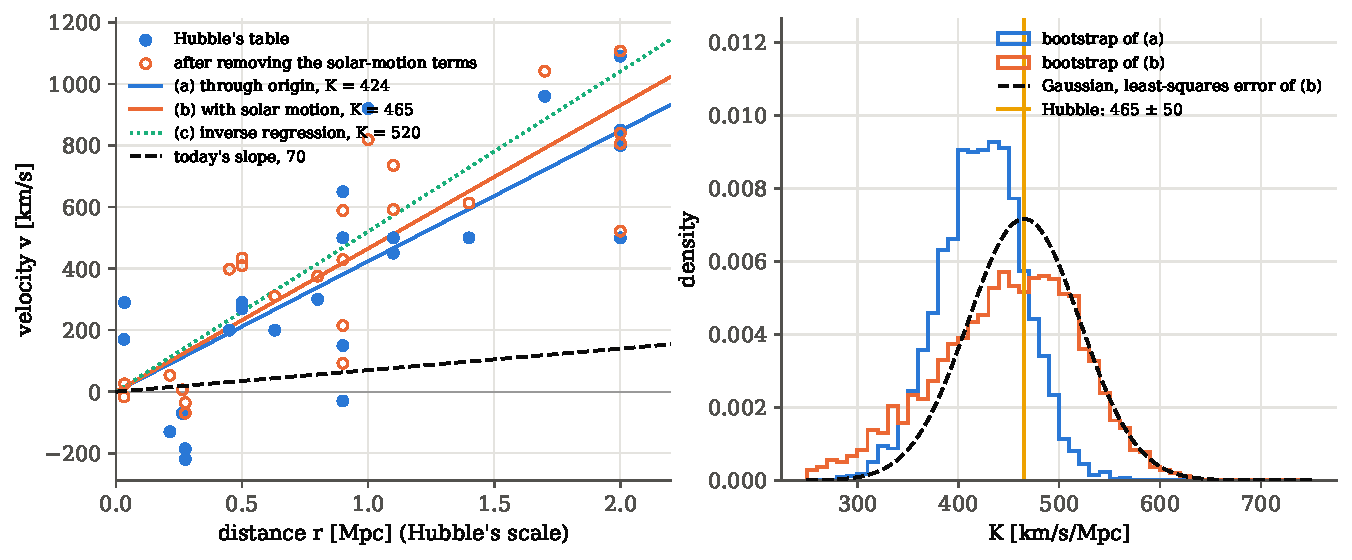
\includegraphics[width=12.5cm]{figures/ch11/hubble1929.pdf}
\caption{Left: Hubble's twenty-four galaxies (filled) and the same velocities with
our fitted solar-motion dipole removed (open). The lines are the slope fitted
through the origin (a), the slope fitted with the solar motion (b), the inverse
regression of distance on velocity (c), and today's slope of $70$ (dashed). Right:
bootstrap distributions of the slopes (a) and (b), the Gaussian implied by the
least-squares error of (b), and Hubble's value.}
\label{11c:fig:hubble1929}
\end{figure}

\paragraph{The error bar from resampling.} The least-squares error assumes
(H2): independent Gaussian peculiar velocities of a common spread. The bootstrap
of \cref{3b:sec:bootstrap} assumes only that the twenty-four galaxies are a fair
sample of galaxies like them: draw twenty-four galaxies from the table with
replacement, refit, repeat $\FBHubNboot$ times. For the slope alone the bootstrap
spread, $\FBHubBootSa$, matches the formula. For the four-parameter fit it is
$\FBHubBootSb$, wider than $\FBHubsKb$ and skewed (\cref{11c:fig:hubble1929}, right):
a resample that happens to contain few galaxies in some part of the sky cannot
pin down the dipole, and the slope wanders with it. With twenty-four points and
four parameters the Gaussian error bar is optimistic.

\subsection{When the distances are noisy too}
\label{11c:sec:hubble-errors}

Hubble's distances were not exact. A distance from the brightest stars of a galaxy
is uncertain by a fixed \emph{fraction}, because the luminosity of the brightest
star varies from galaxy to galaxy and a magnitude error is a fractional distance
error. So now replace the bookkeeping input by a physical one:

\begin{enumerate}[label=(H\arabic*),leftmargin=2.6em,itemsep=1pt,start=4]
  \item \emph{Lognormal distance errors.} The measured distance is
        $r_i^{\rm obs}=r_i\,e^{\eta_i}$ with $\eta_i\sim\Normal(0,\Delta^2)$
        independent of everything else; $\Delta$ is the fractional error.
\end{enumerate}

Two simple limits bracket the answer. If all the noise is in the velocities, we
regress $v$ on $r$, which is \eqref{11c:eq:k-origin}. If all the noise is in the
distances, the roles swap: the velocity is exact, the distance is the noisy
variable, and we should regress $r$ on $v$, $r=bv$, with
$\hat b=\sum_iv_ir_i/\sum_iv_i^2$ by the same chain with $r$ and $v$ exchanged, and
$\hat K=1/\hat b=\sum_iv_i^2/\sum_iv_ir_i=\FBHubKinv$. The two lines differ by more
than twice the error bar of either. The data have not changed; only the assumption
about which number carries the noise has. That is the likelihood at work: it asks
how plausible the noise needed to turn the prediction into the data is, and the
answer depends on where that noise is allowed to sit.

\paragraph{Both noises at once.} The honest model keeps both. To first order in
the small $\eta_i$, $r_i=r_i^{\rm obs}e^{-\eta_i}\approx r_i^{\rm obs}(1-\eta_i)$, so
\begin{align}
  v_i
  &\eqby{1}Kr_i+\epsilon_i
   \eqby{2}Kr_i^{\rm obs}+\bigl(\epsilon_i-Kr_i^{\rm obs}\eta_i\bigr),
  \nonumber\\
  \Var\bigl(v_i\given r_i^{\rm obs}\bigr)
  &\eqby{3}\sigma_v^2+K^2\Delta^2\bigl(r_i^{\rm obs}\bigr)^2\equiv s_i^2(K).
  \label{11c:eq:eff-var}
\end{align}
\begin{explain}
  \item The model (H1)--(H2), without the solar motion for clarity.
  \item Substitute $r_i\approx r_i^{\rm obs}(1-\eta_i)$ and collect the noise.
  \item $\epsilon_i$ and $\eta_i$ are independent, so their variances add; the second
        is multiplied by the square of its coefficient $Kr_i^{\rm obs}$.
\end{explain}
The noise of each point now grows with its distance, and its variance depends on
the parameter $K$ itself. The likelihood is no longer a plain $\chi^2$:
\[
  -2\ln\Like(K,\sigma_v)=\sum_i\Bigl[\frac{\bigl(v_i-Kr_i^{\rm obs}\bigr)^2}{s_i^2(K)}+\ln s_i^2(K)\Bigr]+\text{const},
\]
and the $\ln s_i^2$ term, the normalisation of each Gaussian, must be kept: it
depends on $K$, and dropping it would let the fit lower $\chi^2$ simply by making
$K$, and with it every $s_i$, large. We maximise it numerically over $K$ and $\sigma_v$ at a fixed
$\Delta$. At $\Delta=0$ it returns $\FBHubKmlZero$, the slope through the origin; at
$\Delta=0.2$ (a $0.43$\,mag distance error) $\FBHubKmlTwo$; at $\Delta=0.4$,
$\FBHubKmlFour$. As $\Delta$ grows the distant galaxies are down-weighted, since
their variance $K^2\Delta^2r^2$ grows fastest. The first-order expansion has also
dropped something important: given a measured distance, the true distance is not
equally likely to lie above and below it, because there are more galaxies at
larger distances. That is Malmquist bias, and \cref{11c:sec:ihm} treats it
properly.

\subsection{Why 465 and not 70}
\label{11c:sec:hubble-scale}

None of these fits moves the slope anywhere near $70$. The reason is a property of
the model, not of the estimator. Suppose every distance in the table is too small
by the same factor $c$, so that the true distances are $cr_i$. Refit:
\begin{align}
  \hat K(c\,\bm r)
  &\eqby{1}\frac{\sum_iv_i\,(cr_i)}{\sum_i(cr_i)^2}
   \eqby{2}\frac{1}{c}\,\hat K(\bm r),
  \nonumber\\
  v_i-\hat K(c\,\bm r)\,cr_i
  &\eqby{3}v_i-\hat K(\bm r)\,r_i .
  \label{11c:eq:scale-invisible}
\end{align}
\begin{explain}
  \item \eqref{11c:eq:k-origin} with $r_i$ replaced by $cr_i$.
  \item One factor of $c$ in the numerator, two in the denominator.
  \item The product $\hat K\,r_i$ is unchanged, so every residual is unchanged.
\end{explain}
The residuals, and so $\chi^2_{\min}$, the estimate of $\sigma_v$ and the fractional
error $\sigma_{\hat K}/\hat K$, are identical for every $c$. The data cannot tell
$c=1$ from $c=6.6$; they constrain only the product $Kc$. The error bar on
Hubble's slope ($\pm50$ in his paper, $\pm\FBHubsKb$ in our refit) is an honest statement about the scatter of his points and says
nothing about $c$. This is the $H_0$--$M$ degeneracy of the supernova Hubble
diagram (\cref{3b:sec:hubble-degeneracy}) in its oldest form: a velocity--distance
diagram measures $H_0$ only in units of its distance scale, and the scale has to
come from somewhere else.

How large was the error of the scale? To turn $\FBHubKb$ into $70$, every distance
must grow by $\FBHubKb/70=\FBHubFacb$, which in the language of magnitudes is
$5\log_{10}\FBHubFacb=\FBHubDmub$\,mag: Hubble's standard candles were assumed
about four magnitudes fainter than they are. Hubble placed the Virgo cluster at
$2$\,Mpc; today it is at about $16$\,Mpc. The error was found in pieces. Baade
showed that the Cepheids used to calibrate the period--luminosity relation
belonged to a different stellar population from those in the nebulae, which
doubled the distances \cite{Baade1956}. Sandage showed that many of Hubble's
``brightest stars'' in the more distant galaxies were clouds of ionised gas,
intrinsically much brighter, and by 1958 the slope was near $75$, still uncertain
by a factor of two \cite{Sandage1958}. A further, quieter bias pushed the same way.
The farther galaxies' distances came from the brightest objects that could be
seen in them, and near the limit of a survey the objects that can be seen are the
ones that happen to be unusually bright, so their distances come out too small;
that is the classical Malmquist bias of \cref{T2b:sec:malmquist}. The modern
version of the scale, Cepheids anchored by geometry and carried to supernovae,
is the ladder of \cref{T2b:sec:ladder}.

\paragraph{The lesson.} Refitting Hubble's table reproduces his $465$ to a few
km/s, and shows that the error bar measures the scatter of the points, never the
scale they are plotted on: a common multiplicative error is invisible to the fit
and does not shrink with more galaxies.
\section{Peculiar velocities: what moves the galaxies}
\label{11c:sec:pecvel}

The scatter in Hubble's diagram was $\FBHubSva$\,km/s
(\cref{11c:sec:hubble-model}), and Andromeda, our nearest large neighbour, comes
towards us at $220$\,km/s against the general recession. In the refit of
\cref{11c:sec:hubble1929} these peculiar velocities were noise: independent random
numbers $\epsilon_i$ with a spread $\sigma_v$ to be estimated from the residuals.
They are not random in that sense. A galaxy moves because the matter around it
pulls on it, and two neighbouring galaxies feel nearly the same pull. Once we know
what produces the velocities, three things follow: how large they are in a
universe with the measured power spectrum, how strongly the velocities of two
galaxies a distance $r$ apart are correlated, and, in the next two sections, what
they do to every measurement of the local expansion.

\paragraph{The question.}
\begin{enumerate}
  \item How is a peculiar velocity read off from a redshift and a distance?
  \item Given the density contrast everywhere, what is the velocity at one point?
  \item How large is the typical velocity today, for the CAMB power spectrum, and
        which scales produce it?
  \item How correlated are the velocities of two galaxies a distance $r$ apart?
\end{enumerate}

\subsection{Reading a peculiar velocity from a redshift}
\label{11c:sec:pv-redshift}

A galaxy's redshift has two causes, composed one after the other
(\cref{11a:sec:rsd-map}, \eqref{11a:eq:z-compose}): the expansion stretches the light
by $1+z_c$, where $z_c$ is the \newterm{cosmological redshift} the galaxy would have
at rest, and its own line-of-sight velocity $u_r$ Doppler-shifts it by $1+u_r/c$.
Solving for $u_r$,
\begin{align}
  1+z_{\rm obs}=(1+z_c)\Bigl(1+\frac{u_r}{c}\Bigr)
  \quad\Longrightarrow\quad
  u_r
  &\eqby{1}c\,\frac{(1+z_{\rm obs})-(1+z_c)}{1+z_c}
   \eqby{2}c\,\frac{z_{\rm obs}-z_c}{1+z_c},
  \label{11c:eq:vpec-z}
\end{align}
\begin{explain}
  \item Divide by $1+z_c$, subtract $1$, multiply by $c$.
  \item The ones cancel in the numerator.
\end{explain}
which is the definition Hogg uses \cite[eq.~(10)]{Hogg1999}. Near us
$z_c\ll1$ and $cz_c=H_0r$, so $cz_{\rm obs}\approx H_0r+u_r$: the observed
recession velocity is the Hubble flow plus the line-of-sight peculiar velocity.
That is the model of \cref{11c:sec:hubble-model}, with $\epsilon_i$ renamed
$u_{r,i}$.

To measure $u_r$ for one galaxy we therefore need its distance from something
other than its redshift: a Cepheid, a supernova, the Tully--Fisher relation. The
error of $u_r=cz_{\rm obs}-H_0r$ is then $H_0\sigma_r$, and it grows with distance.

\paragraph{Example: how far out can one velocity be measured?} A Tully--Fisher
distance is uncertain by about $20\%$. At $r=10$\,Mpc, with $H_0=70$\,km/s/Mpc, the
velocity error is $70\times0.2\times10=140$\,km/s, smaller than the $300$\,km/s we
will find for a typical peculiar velocity. At $50$\,Mpc it is $700$\,km/s, larger.
Beyond a few tens of megaparsecs individual peculiar velocities are lost in the
distance errors, and only averages over many galaxies survive. That is why the
local Universe is the place where velocities are data.

\subsection{The velocity field of linear theory}
\label{11c:sec:pv-linear}

\emph{Inputs.} We take two results of cosmological perturbation theory as given
(see the cosmology notes); they are the same inputs as in the redshift-space
distortions of \cref{11a:sec:kaiser}.
\begin{enumerate}[label=(V\arabic*),leftmargin=2.6em,itemsep=1pt]
  \item \emph{Linear continuity.} With $\bm u$ the peculiar velocity, $a$ the scale
        factor, $H$ the expansion rate, $\delta$ the matter density contrast and
        $f=\dd\ln D/\dd\ln a$ the growth rate,
        $\nabla\cdot\bm u=-aHf\,\delta$, which is \eqref{11a:eq:theta} multiplied by
        $aH$. Matter flows out of regions where the density falls.
  \item \emph{No curl.} Rotational velocity perturbations decay as the Universe
        expands, so $\nabla\times\bm u=0$ on large scales.
\end{enumerate}
\emph{The question:} given $\delta$ everywhere, what is $\bm u$ at the point $\bm x$?

\emph{A field without curl is a gradient.} Write $\bm u=\nabla\psi$. Then (V1) is an
equation for $\psi$ alone, $\nabla^2\psi=-aHf\,\delta$: Poisson's equation, with
$-aHf\,\delta$ as the source. We solve it the way one solves for an electrostatic
potential, with the potential of a point source.

\emph{The point source.} Away from the origin, with $\rho=|\bm x|$,
$\nabla^2(1/\rho)=\rho^{-2}\,\dd/\dd\rho\,\bigl(\rho^2\,\dd(1/\rho)/\dd\rho\bigr)
=\rho^{-2}\,\dd(-1)/\dd\rho=0$. At the origin it is singular, and its strength
follows from the divergence theorem: the flux of $\nabla(1/\rho)=-\hat{\bm\rho}/\rho^2$
out of a sphere of any radius $\varepsilon$ is $(-1/\varepsilon^2)(4\pi\varepsilon^2)=-4\pi$.
So $\nabla^2(1/\rho)$ is zero everywhere except at the origin and integrates to
$-4\pi$ over any ball around it:
$\nabla^2\bigl(1/|\bm x-\bm x'|\bigr)=-4\pi\,\delta_D(\bm x-\bm x')$, with $\delta_D$ the
Dirac delta.

\emph{Superpose.} A sum of point sources solves Poisson's equation for the summed
source. Hence
\begin{align}
  \psi(\bm x)
  &\eqby{1}\frac{aHf}{4\pi}\int\dd^3x'\,\frac{\delta(\bm x')}{|\bm x-\bm x'|},
  \nonumber\\
  \bm u(\bm x)=\nabla\psi
  &\eqby{2}\frac{aHf}{4\pi}\int\dd^3x'\,\delta(\bm x')\,
   \frac{\bm x'-\bm x}{|\bm x'-\bm x|^3}.
  \label{11c:eq:u-integral}
\end{align}
\begin{explain}
  \item Check: $\nabla^2\psi=\frac{aHf}{4\pi}\int\dd^3x'\,\delta(\bm x')\,
        \bigl(-4\pi\delta_D(\bm x-\bm x')\bigr)=-aHf\,\delta(\bm x)$, which is (V1).
  \item $\nabla_{\bm x}|\bm x-\bm x'|^{-1}=-(\bm x-\bm x')/|\bm x-\bm x'|^3$; the
        gradient acts on $\bm x$, not on the integration variable.
\end{explain}

\begin{keyidea}[The linear velocity field]
In linear theory the peculiar velocity at $\bm x$ is
$\bm u(\bm x)=\frac{aHf}{4\pi}\int\dd^3x'\,\delta(\bm x')\,(\bm x'-\bm x)/|\bm x'-\bm x|^3$
\cite{Kaiser1987,Peebles1993}: every overdense patch pulls with an inverse-square
law, and the velocity points along the total pull. In Fourier space it is
$\bm u_{\bm k}=i\,aHf\,\bm k\,\delta_{\bm k}/k^2$, the relation used for redshift-space
distortions in \eqref{11a:eq:dvdz}.
\end{keyidea}

The integral is Newton's gravitational field of the excess mass $\bar\rho\,\delta$,
up to a constant. The velocity is parallel to the peculiar gravitational
acceleration: in linear theory a galaxy moves in the direction it is pulled. The
inverse-square fall-off is offset by the volume of a shell, which grows as the
square of its radius, so distant matter is not negligible. A shell of uniform
excess pulls equally in all directions and contributes nothing, but a shell whose
density differs between one side and the other contributes as much as a nearby
clump of the same total mass excess.

\paragraph{Example: one density wave.} Take $\delta(\bm x)=A\cos(\bm k\cdot\bm x)$
with a small amplitude $A$. The Fourier form gives
$\bm u=-aHf\,A\,(\bm k/k^2)\sin(\bm k\cdot\bm x)$: a velocity along $\bm k$, a quarter
wavelength out of step with the density, with amplitude $aHfA/k=aHfA\lambda/2\pi$.
Matter flows from the troughs towards the crests. For the same density amplitude,
a longer wave gives a faster flow, in proportion to its wavelength. With $aH=100$
km/s per $h^{-1}$Mpc today, $f=\FBPvF$, $A=0.05$ and $\lambda=100\,h^{-1}$Mpc, the
flow amplitude is $100\times\FBPvF\times0.05\times100/(2\pi)\approx42$\,km/s.

\subsection{How fast, on average}
\label{11c:sec:pv-sigma}

The density contrast on large scales is a Gaussian random field with power spectrum
$P(k)$ (\cref{7a:sec:grf-fourier}): $\langle\delta_{\bm k}\rangle=0$ and
$\langle\delta_{\bm k}\delta^*_{\bm k'}\rangle=(2\pi)^3\delta_D(\bm k-\bm k')P(k)$, with
$\delta(\bm x)=\int\frac{\dd^3k}{(2\pi)^3}\delta_{\bm k}e^{i\bm k\cdot\bm x}$. The
velocity is a linear function of $\delta$, and a linear function of a Gaussian
field is a Gaussian field (\cref{7a:sec:grf}). So each velocity component is
Gaussian with mean zero, and all we need is its covariance. For components $i$
and $j$ at two points separated by $\bm r$,
\begin{align}
  \bigl\langle u_i(\bm x)\,u_j(\bm x+\bm r)\bigr\rangle
  &\eqby{1}\int\!\!\frac{\dd^3k}{(2\pi)^3}\!\int\!\!\frac{\dd^3k'}{(2\pi)^3}\,
   \bigl\langle u_{i,\bm k}\,u^*_{j,\bm k'}\bigr\rangle\,
   e^{i\bm k\cdot\bm x-i\bm k'\cdot(\bm x+\bm r)}
  \nonumber\\
  &\eqby{2}(aHf)^2\!\int\!\!\frac{\dd^3k}{(2\pi)^3}\!\int\!\!\frac{\dd^3k'}{(2\pi)^3}\,
   \frac{k_ik'_j}{k^2k'^2}\,(2\pi)^3\delta_D(\bm k-\bm k')P(k)\,
   e^{i\bm k\cdot\bm x-i\bm k'\cdot(\bm x+\bm r)}
  \nonumber\\
  &\eqby{3}(aHf)^2\int\frac{\dd^3k}{(2\pi)^3}\,P(k)\,\frac{k_ik_j}{k^4}\,e^{i\bm k\cdot\bm r}.
  \label{11c:eq:vel-cov}
\end{align}
\begin{explain}
  \item $u_j$ is real, so we may write it as its own complex conjugate,
        $u_j(\bm y)=\int\frac{\dd^3k'}{(2\pi)^3}u^*_{j,\bm k'}e^{-i\bm k'\cdot\bm y}$;
        the average passes inside the integrals.
  \item $u_{i,\bm k}=iaHf\,k_i\delta_{\bm k}/k^2$ and
        $u^*_{j,\bm k'}=-iaHf\,k'_j\delta^*_{\bm k'}/k'^2$; the factors $i$ and $-i$
        multiply to $1$; then the spectrum of $\delta$.
  \item The delta function sets $\bm k'=\bm k$ and cancels one $(2\pi)^3$; the
        $\bm x$ dependence cancels, as homogeneity requires. The sign of the exponent
        is immaterial because the rest of the integrand is even in $\bm k$.
\end{explain}

\emph{One point.} At $\bm r=0$, sum over $i=j$: $k_ik_i=k^2$, and with
$\dd^3k=4\pi k^2\dd k$ for an isotropic integrand,
\begin{equation}
  \sigma_v^2\equiv\bigl\langle|\bm u|^2\bigr\rangle
  =(aHf)^2\int\frac{4\pi k^2\,\dd k}{(2\pi)^3}\,\frac{P(k)}{k^2}
  =\frac{(aHf)^2}{2\pi^2}\int_0^\infty P(k)\,\dd k ,
  \qquad
  \sigma_{v,1\mathrm D}^2=\frac{\sigma_v^2}{3},
  \label{11c:eq:sigma-v}
\end{equation}
the second because isotropy shares the three components equally. Compare the
density variance in a sphere of radius $R$ (\cref{7a:sec:smoothing}),
$\sigma_R^2=\frac{1}{2\pi^2}\int k^2P(k)\,W^2(kR)\,\dd k$: the velocity carries two
fewer powers of $k$. That is the wave example again: velocity grows with
wavelength, so velocities are made by larger scales than densities.

\paragraph{Example: the numbers today.} Script
\pyname{code/ch11/09_peculiar_velocities.py} integrates \eqref{11c:eq:sigma-v} with the
CAMB linear spectrum at $z=0$ (the one of \cref{T1a:sec:pk}, $\sigma_8=\FBPvSigEight$)
and $f=\FBPvF$. Lengths are in $h^{-1}$Mpc, so $aH=100$\,km/s per $h^{-1}$Mpc and
$h$ drops out. It finds $\sigma_v=\FBPvSigThree$\,km/s in three dimensions and
$\sigma_{v,1\mathrm D}=\FBPvSigOne$\,km/s along one line of sight: the
``$\sim300$\,km/s'' assumed for the peculiar velocities of supernova hosts in
\cref{3b:sec:hubble-model} and \cref{T2b:sec:snia}. \Cref{11c:fig:pecvel-theory} (left)
shows where it comes from. Half of $\sigma_v^2$ comes from $k<\FBPvKhalfV\,h$/Mpc,
wavelengths longer than $\FBPvLhalfV\,h^{-1}$Mpc, while half of $\sigma_8^2$ comes from
$k<\FBPvKhalfD$, wavelengths longer than $\FBPvLhalfD\,h^{-1}$Mpc. A galaxy's velocity is
set by the distribution of mass over a region several times larger than the
region that sets its local density.

This number is the velocity of the smooth large-scale flow. Galaxies inside groups
and clusters also orbit in the group's potential, at up to $1000$\,km/s in rich
clusters; linear theory knows nothing of that, and it adds a non-Gaussian,
small-scale part on top of \eqref{11c:eq:sigma-v}.

\begin{figure}[htbp]
\centering
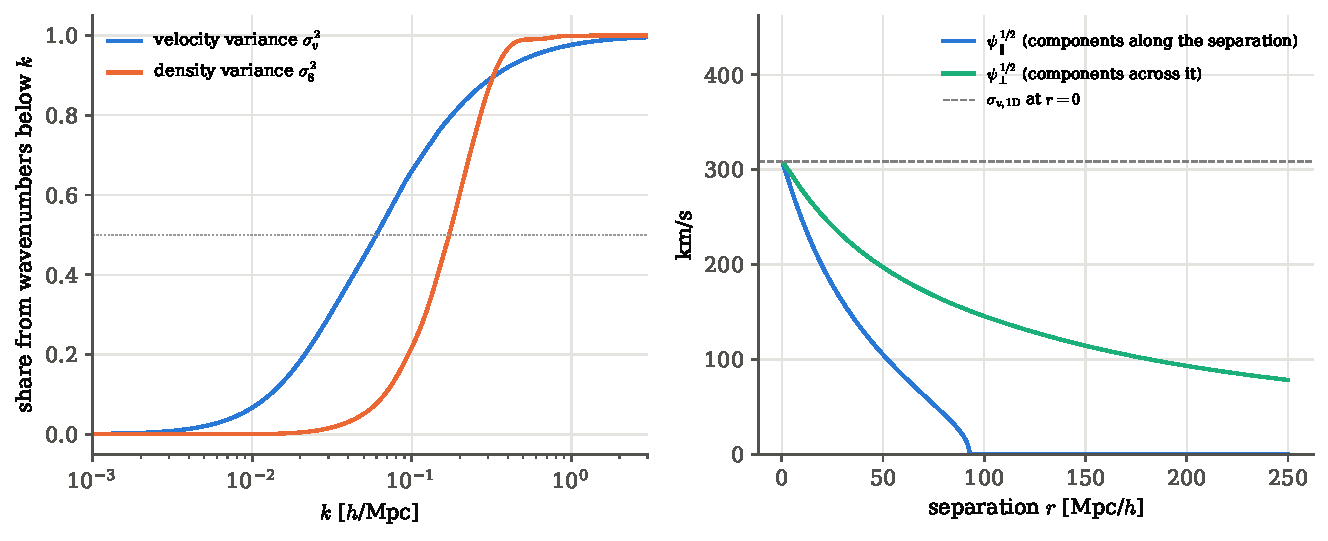
\includegraphics[width=12.5cm]{figures/ch11/pecvel_theory.pdf}
\caption{Left: the share of the velocity variance $\sigma_v^2$ and of the density
variance $\sigma_8^2$ contributed by wavenumbers below $k$; velocities come from
about three times larger scales. Right: the square roots of the velocity
correlation functions for components along the separation ($\psi_\parallel$) and
across it ($\psi_\perp$); both start at the one-dimensional rms velocity, and
$\psi_\perp$ is still half of it at $100\,h^{-1}$Mpc.}
\label{11c:fig:pecvel-theory}
\end{figure}

\subsection{How correlated: the velocity correlation functions}
\label{11c:sec:pv-corr}

Now keep $\bm r\neq0$ in \eqref{11c:eq:vel-cov}. Isotropy says the answer can only be
built from $\delta_{ij}$ and $\hat r_i\hat r_j$: the component of velocity along the
separation and the components across it are the only distinguishable directions.
So we need the angular average of $\hat k_i\hat k_j\,e^{i\bm k\cdot\bm r}$ over the
directions of $\bm k$.

\emph{Start from the simplest average.} Without the factors $\hat k_i\hat k_j$ the
average over directions is a familiar integral: with $\mu$ the cosine of the angle
between $\bm k$ and $\bm r$ and $x=kr$,
$\frac{1}{4\pi}\int\dd\Omega_k\,e^{i\bm k\cdot\bm r}=\frac12\int_{-1}^1e^{ix\mu}\dd\mu
=\frac{\sin x}{x}=j_0(x)$, the spherical Bessel function of order zero.

\emph{Bring down the factors by differentiating.} Each derivative $\partial/\partial r_i$
of $e^{i\bm k\cdot\bm r}$ brings down $ik_i$, so $k_ik_j\,e^{i\bm k\cdot\bm r}=
-\partial_i\partial_je^{i\bm k\cdot\bm r}$, and the angular average of $k_ik_je^{i\bm k\cdot\bm r}$
is $-\partial_i\partial_j\,j_0(kr)$. For a function $g(r)$ of $r=|\bm r|$ alone,
$\partial_ig=g'\hat r_i$ and $\partial_j\hat r_i=(\delta_{ij}-\hat r_i\hat r_j)/r$, so
\begin{align}
  -\partial_i\partial_j\,j_0(kr)
  &\eqby{1}-\Bigl[g''\,\hat r_i\hat r_j+\frac{g'}{r}\bigl(\delta_{ij}-\hat r_i\hat r_j\bigr)\Bigr]_{g=j_0(kr)}
  \nonumber\\
  &\eqby{2}k^2\Bigl[\Bigl(j_0(x)-\frac{2j_1(x)}{x}\Bigr)\hat r_i\hat r_j
   +\frac{j_1(x)}{x}\bigl(\delta_{ij}-\hat r_i\hat r_j\bigr)\Bigr],
  \nonumber\\
  \frac{1}{4\pi}\int\dd\Omega_k\,\hat k_i\hat k_j\,e^{i\bm k\cdot\bm r}
  &\eqby{3}\frac{j_1(x)}{x}\,\delta_{ij}+\Bigl(j_0(x)-\frac{3j_1(x)}{x}\Bigr)\hat r_i\hat r_j .
  \label{11c:eq:angular}
\end{align}
\begin{explain}
  \item The product rule on $\partial_j(g'\hat r_i)$.
  \item $j_0'(x)=-j_1(x)$ and $j_1'(x)=j_0(x)-2j_1(x)/x$, with
        $j_1(x)=\sin x/x^2-\cos x/x$; so $g'=-kj_1$, $g''=-k^2\bigl(j_0-2j_1/x\bigr)$, and
        $g'/r=-k^2j_1/x$.
  \item Divide by $k^2$ (since $k_ik_j=k^2\hat k_i\hat k_j$) and collect the
        $\hat r_i\hat r_j$ terms: $j_0-2j_1/x-j_1/x$.
\end{explain}
A check: at $r\to0$, $j_1(x)/x\to1/3$ and $j_0\to1$, so the average becomes
$\delta_{ij}/3$, the average of $\hat k_i\hat k_j$ over all directions. Putting
\eqref{11c:eq:angular} into \eqref{11c:eq:vel-cov} with $\dd^3k=k^2\dd k\,\dd\Omega_k$, the
$k^2$ cancels the $k^2$ left in $k_ik_j/k^4=\hat k_i\hat k_j/k^2$, and for the
components across and along the separation (take $i=j$ perpendicular to $\hat{\bm r}$,
or $i=j$ along it):
\begin{equation}
  \psi_\perp(r)=\frac{(aHf)^2}{2\pi^2}\int_0^\infty\!\dd k\,P(k)\,\frac{j_1(kr)}{kr},
  \qquad
  \psi_\parallel(r)=\frac{(aHf)^2}{2\pi^2}\int_0^\infty\!\dd k\,P(k)
  \Bigl[j_0(kr)-\frac{2j_1(kr)}{kr}\Bigr],
  \label{11c:eq:psi}
\end{equation}
the two velocity correlation functions of G\'orski \cite{Gorski1988}. Both equal
$\sigma_{v,1\mathrm D}^2$ at $r=0$.

\Cref{11c:fig:pecvel-theory} (right) shows them. At $r=100\,h^{-1}$Mpc,
$\psi_\perp^{1/2}=\FBPvPerpHundred$\,km/s: two galaxies a hundred megaparsecs apart
still share about half of their typical transverse velocity. Large regions move
together, in \newterm{bulk flows}. $\psi_\parallel$ falls faster and turns slightly
negative: the components along the separation of two distant galaxies tend to
have opposite signs, as they do on the two sides of a region into which matter is
falling, or out of which it is streaming.

\begin{pitfall}[Peculiar velocities are not independent noise]
Model (H2) of \cref{11c:sec:hubble-model} treated the peculiar velocities of
Hubble's galaxies as independent. Within a few tens of megaparsecs they are almost
perfectly correlated. A sample of nearby galaxies shares a common flow, which does
not average away as $1/\sqrt N$: it shifts every velocity the same way. The part of
the common flow that grows linearly with distance looks exactly like a change of
the Hubble constant (\cref{11c:sec:cosmicvar}).
\end{pitfall}

\subsection{Velocities in a simulated box}
\label{11c:sec:pv-box}

The derivation assumed a Gaussian field with the CAMB spectrum. We now build such a
field and check both results. Script \pyname{code/ch11/09_peculiar_velocities.py}
draws $\FBPvNbox$ boxes of side $\FBPvBoxL\,h^{-1}$Mpc with $\FBPvBoxN^3$ cells,
using the grid conventions of \cref{7a:sec:box}, and computes the velocity from the
Fourier form of the key idea:

\pyfile[firstline=103,lastline=110,firstnumber=103]{code/ch11/09_peculiar_velocities.py}{Velocity components from a Gaussian density field, and their one- and two-point averages}

\noindent Line 104 colours white noise with $\sqrt{P(k)}$, which makes
\pyname{dk} the Fourier transform of a Gaussian field with spectrum $P$ on the grid.
Lines 105--106 multiply by $iaHf\,k_x/k^2$ and $iaHf\,k_y/k^2$ (with $aH=100$ and
$1/k^2$ set to zero for the $\bm k=0$ mode) and transform back: these are $u_x$ and
$u_y$ in km/s. Line 107 records the one-point variance. Lines 108--109 shift the
field along $x$ by $n$ cells and average the products: $u_x$ with $u_x$ is
$\psi_\parallel$ at separation $n\times\FBPvBoxL/\FBPvBoxN\,h^{-1}$Mpc, and $u_y$ with
$u_y$ is $\psi_\perp$.

The theory to compare with is \eqref{11c:eq:vel-cov} restricted to the modes the box
contains: the integral over $\bm k$ becomes a sum over the grid modes, divided by the
volume (\cref{7a:sec:box}). It gives $\sigma_{v,1\mathrm D}=\FBPvSigOneGrid$\,km/s;
the boxes give $\FBPvSigOneBox\pm\FBPvSigOneBoxScatter$, where the $\pm$ is the
box-to-box scatter. Both are below the $\FBPvSigOne$ of the full integral because the
box has no waves longer than $\FBPvBoxL\,h^{-1}$Mpc, and \cref{11c:fig:pecvel-theory}
showed that such waves carry a few per cent of $\sigma_v^2$. The histogram of $u_x$ is
Gaussian, and the correlation functions follow the grid-mode sums
(\cref{11c:fig:pecvel-box}). The points at large separations sit a little below the
curves, by about one box-to-box scatter: with four boxes, the longest waves are
sampled only a handful of times, which is the sample variance of
\cref{7a:sec:sample-var} acting on a quantity dominated by large scales.

\begin{figure}[htbp]
\centering
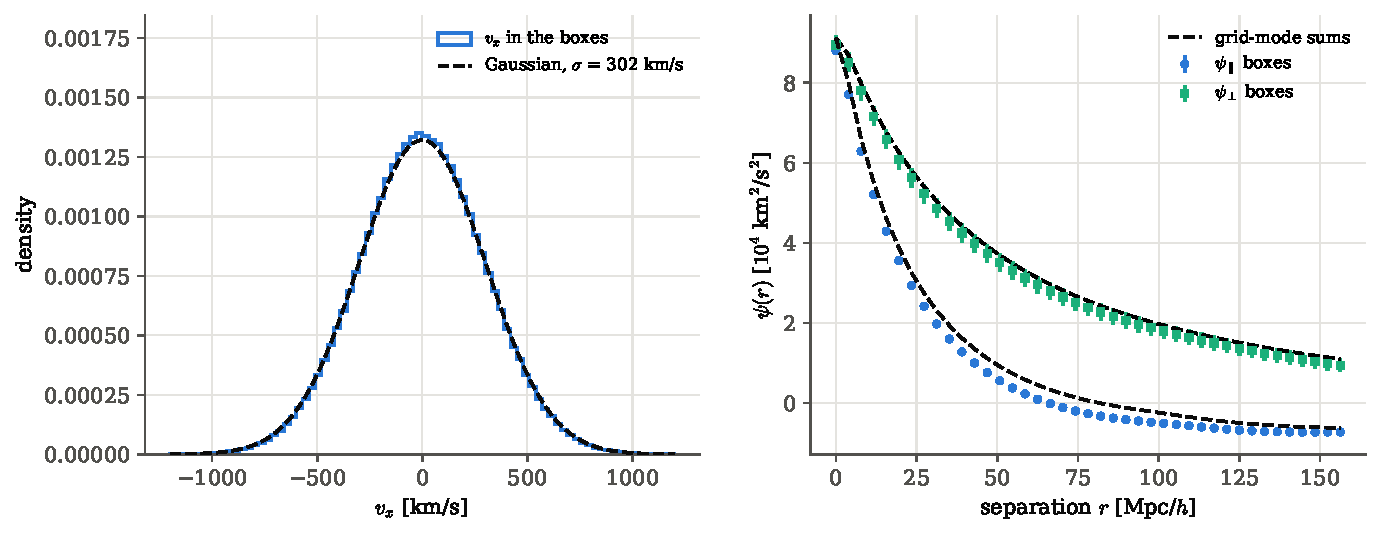
\includegraphics[width=12.5cm]{figures/ch11/pecvel_box.pdf}
\caption{Velocities in Gaussian boxes. Left: the distribution of one velocity
component against a Gaussian of the predicted width. Right: the two velocity
correlation functions measured in the boxes (points, with the error of the mean of
four boxes) and the corresponding sums over the box's Fourier modes (dashed).}
\label{11c:fig:pecvel-box}
\end{figure}

\paragraph{The lesson.} Peculiar velocities are the gradient of a potential sourced
by the density contrast; that makes them Gaussian, about $300$\,km/s along a line of
sight today, and coherent over a hundred megaparsecs, because they are made by
longer waves than the densities are.
\section{The local flow: falling towards Virgo}
\label{11c:sec:virgo}

Four of Hubble's twenty-four galaxies were in the Virgo cluster, the nearest rich
cluster, a few hundred galaxies at about $16$\,Mpc. A mass of that size pulls on
everything around it, us included. Galaxies between us and Virgo are pulled away
from us, towards the cluster; galaxies beyond it are pulled towards us. We
ourselves fall towards Virgo, so every velocity we measure is measured from a
moving platform. A measurement of $H_0$ from nearby galaxies that ignores all this
fits a straight line to a pattern that is not straight. The linear velocity field
of \cref{11c:sec:pecvel} turns the pattern into a model with one extra parameter,
our infall speed, which can be fitted together with $H_0$.

\emph{Where we have met $H_0$ before.} Every fit of $H_0$ so far treated peculiar
velocities as noise. The mock supernovae of \cref{3b:sec:hubble-model}, made with
$H_0=70$, carried independent Gaussian velocities of $300$\,km/s, and Hubble's
twenty-four nebulae (\cref{11c:sec:hubble1929}) left residuals of $200$ to
$230$\,km/s that we fitted as an independent scatter, with only the Sun's motion
modelled, as a dipole. The real ladder of \cref{T2b:sec:ladder} avoids the problem
rather than modelling it: its Hubble-flow supernovae start at $z=0.023$, about
$7000$\,km/s, where a velocity of $250$\,km/s shifts a distance modulus by less than
$0.1$\,mag \eqref{T2b:eq:mu-pec}. Here the galaxies lie within $30$\,Mpc, where the
whole recession is at most a couple of thousand km/s and a coherent infall of
$200$\,km/s is not small, so the velocities move from the noise into the model. The
estimator is the same weighted least squares, now with two columns, $H_0$ and the
infall speed, and the data are mock again, made with $H_0=70$ as in
\cref{3b:sec:hubble}, so the question is once more whether a fit recovers a known
truth. The low value it returns when the infall is ignored is therefore not a third
measurement to set beside $73.04$ and $67.36$: it is the size of an omitted-variable
bias, a measure of how far a local fit can miss without a model of the flow.

\paragraph{The question.}
\begin{enumerate}
  \item What velocity field does linear theory predict around a spherical
        overdensity?
  \item What does an observer who is falling into it measure for the radial
        velocities of galaxies around them?
  \item Can $H_0$ and the infall speed be fitted together from a local sample, and
        what goes wrong if the infall is ignored, or if the distances are poor?
  \item How fast does the Local Group move with respect to the CMB, and how much of
        that is Virgo?
\end{enumerate}

\subsection{Infall around a spherical overdensity}
\label{11c:sec:infall}

Take a density contrast $\delta$ that is spherically symmetric about a centre, the
cluster. Let $\bm R$ be the vector from the centre to a point, $R=|\bm R|$, and
$\bar\delta(<R)$ the mean contrast inside the sphere of radius $R$. By symmetry the
linear velocity $\bm u$ of \cref{11c:sec:pv-linear} points along $\pm\hat{\bm R}$ and
its size $u_R$ depends only on $R$. Integrate the continuity equation (V1),
$\nabla\cdot\bm u=-aHf\,\delta$, over the ball of radius $R$:
\begin{align}
  4\pi R^2\,u_R(R)
  &\eqby{1}\oint_{|\bm R'|=R}\bm u\cdot\dd\bm S
   \eqby{2}\int_{|\bm R'|<R}\nabla\cdot\bm u\;\dd^3R'
   \eqby{3}-aHf\,\frac{4\pi}{3}R^3\,\bar\delta(<R),
  \nonumber\\
  u_R(R)
  &=-\frac{aHf}{3}\,\bar\delta(<R)\,R .
  \label{11c:eq:infall}
\end{align}
\begin{explain}
  \item The velocity is radial and has the same size everywhere on the sphere, so
        the flux is $u_R$ times the area.
  \item The divergence theorem.
  \item (V1), and the definition of the mean contrast:
        $\int_{<R}\delta\,\dd^3R'=\tfrac{4\pi}{3}R^3\bar\delta(<R)$.
\end{explain}
This is Newton's shell theorem in the language of velocities: only the excess
inside $R$ matters. An overdensity ($\bar\delta>0$) gives an inflow, a void an
outflow. Inside a region of uniform contrast the flow is $-\tfrac13aHf\bar\delta\,\bm R$,
a change of the local expansion rate by $-\tfrac13f\bar\delta$ in units of $H$: the
local-void formula \eqref{T2b:eq:void}, which we derived for the H$_0$ tension in
\cref{T2b:sec:ladder} and will meet again in \cref{11c:sec:cosmicvar}.

\paragraph{A power-law cluster.} Around a cluster the mean contrast falls with
radius. Model it as a power law, $\bar\delta(<R)\propto R^{-2}$, the shape used in
classical models of the Virgocentric flow \cite{Schechter1980}. Then
\eqref{11c:eq:infall} gives a speed that falls as $1/R$. We name the constant by
the infall speed of the Local Group, which sits at $R=d_V$, the distance of Virgo:
\begin{equation}
  \bm u(\bm x)=-v_{\rm inf}\,\frac{d_V}{R}\,\hat{\bm R},
  \qquad
  v_{\rm inf}=\frac{H_0f}{3}\,\bar\delta(<d_V)\,d_V .
  \label{11c:eq:virgo-model}
\end{equation}

\paragraph{Example: how overdense is our neighbourhood?} Literature values of our
infall into Virgo lie around $200$\,km/s. With $H_0=70$, $f=0.53$ and $d_V=16.5$\,Mpc,
\eqref{11c:eq:virgo-model} gives
$\bar\delta(<d_V)=3\times200/(70\times0.53\times16.5)\approx1.0$: the sphere
centred on Virgo and reaching out to us contains about twice the mean density. A
contrast of order one is the edge of linear theory. The model is good for the
general shape of the flow and its dependence on $H_0$; it is not accurate near the
cluster, where $\bar\delta\gg1$, and we exclude galaxies closer than $5$\,Mpc to the
centre.

\subsection{What a falling observer sees}
\label{11c:sec:infall-observer}

We sit at the origin and move with the Local Group. A galaxy at position $\bm x$, at
distance $r=|\bm x|$ in the direction $\hat{\bm r}$, moves with the Hubble flow,
$H_0\bm x$ relative to us, plus its own peculiar velocity $\bm u(\bm x)$. We
measure velocities relative to ourselves, and we have peculiar velocity $\bm u(0)$.
The radial velocity we record is therefore
\begin{align}
  v_{\rm obs}
  &\eqby{1}\bigl[H_0\bm x+\bm u(\bm x)-\bm u(0)\bigr]\cdot\hat{\bm r}
   \eqby{2}H_0r+v_{\rm inf}\,g(\bm x),
  \nonumber\\
  g(\bm x)
  &\equiv\Bigl[-\frac{d_V}{R}\,\hat{\bm R}-\hat{\bm s}_V\Bigr]\cdot\hat{\bm r},
  \qquad \bm R=\bm x-d_V\hat{\bm s}_V .
  \label{11c:eq:vobs-virgo}
\end{align}
\begin{explain}
  \item Velocities relative to a moving platform are differences; only the radial
        component is measured from the Doppler shift.
  \item $\bm x\cdot\hat{\bm r}=r$; insert \eqref{11c:eq:virgo-model}, and note that at the
        origin $\bm R=-d_V\hat{\bm s}_V$, with $\hat{\bm s}_V$ the unit vector from us to
        Virgo, so $\bm u(0)=v_{\rm inf}\hat{\bm s}_V$: we fall towards the cluster.
\end{explain}
The function $g$ is fixed by geometry once the position of Virgo is known
(\cref{11c:fig:virgo-geometry}). It has two parts. The second, $-\hat{\bm s}_V\cdot\hat{\bm r}$,
is the reflex of our own fall, a dipole on the sky exactly like the solar motion of
\cref{11c:sec:hubble-model}. The first is the pattern of the other galaxies' fall
towards the cluster: positive in front of Virgo, where galaxies are pulled away
from us, and negative behind it, where they are pulled towards us. Along the line
of sight through Virgo the two together give the S-shaped curve in
\cref{11c:fig:virgo-infall} (left, red).

\begin{figure}[htbp]
\centering
\begin{tikzpicture}[scale=1.0]
  \coordinate (O) at (0,0);
  \coordinate (V) at (5,0);
  \coordinate (G) at (6.6,1.8);
  \fill[bdryred!15] (V) circle (0.9);
  \fill[bdryred] (V) circle (2.5pt);
  \node[anchor=north,font=\small] at (5,-0.95) {Virgo};
  \fill[black] (O) circle (2pt);
  \node[anchor=east,font=\small] at (-0.1,0) {us};
  \fill[formblue] (G) circle (2.5pt);
  \node[anchor=west,font=\small] at (6.7,1.85) {galaxy at $\bm x$};
  \draw[->,thick] (O) -- (G);
  \node[anchor=south east,font=\small] at (3.2,1.0) {$\bm x=r\hat{\bm r}$};
  \draw[->,thick,faint] (V) -- (G);
  \node[anchor=north west,font=\small] at (5.9,0.85) {$\bm R$};
  \draw[->,very thick,tangentgreen] (G) -- ($(G)!0.9cm!(V)$);
  \node[anchor=north,font=\small,tangentgreen!70!black] at (6.75,1.3) {$\bm u(\bm x)$};
  \draw[->,very thick,tangentgreen] (O) -- (1.1,0);
  \node[anchor=south,font=\small,tangentgreen!70!black] at (0.55,0.08) {$\bm u(0)$};
  \draw[dashed,faint] (1.1,0) -- (V);
\end{tikzpicture}
\caption{The geometry of the Virgocentric flow. Every galaxy, and we ourselves,
fall towards the cluster with a speed that falls off as $1/R$. The velocity we
record for a galaxy is the radial part of its Hubble velocity plus the difference
between its fall $\bm u(\bm x)$ and ours $\bm u(0)$.}
\label{11c:fig:virgo-geometry}
\end{figure}

\paragraph{A model linear in its parameters.} Equation \eqref{11c:eq:vobs-virgo} is
linear in the two unknowns $(H_0,v_{\rm inf})$, with known regressors $r_i$ and
$g_i=g(\bm x_i)$. It is the solar-motion fit of \cref{11c:sec:hubble-model} with a
different second column. The noise has two parts. The galaxies' own motions about
the smooth flow are small near us: within about ten megaparsecs, galaxies scatter
around the local expansion by only some tens of km/s, a surprisingly ``cold''
flow, and we take $\sigma_{\rm th}=\FBViSigth$\,km/s. The distances carry
fractional errors $\Delta$, which by \eqref{11c:eq:eff-var} add
$(H_0\Delta r_i)^2$ to the variance. So the fit is weighted least squares with
$w_i=1/\bigl(\sigma_{\rm th}^2+H_0^2\Delta^2r_i^2\bigr)$: solve the $2\times2$ normal
equations $A^{\mathsf T}WA\,\hat{\bm p}=A^{\mathsf T}W\bm v$, with rows $(r_i,g_i)$ in $A$
and $W=\mathrm{diag}(w_i)$, put the new $\hat H_0$ into the weights, and repeat until
it stops changing; the covariance is $(A^{\mathsf T}WA)^{-1}$
(\cref{3b:sec:correlated}).

\subsection{A simulated local sample}
\label{11c:sec:infall-sim}

Script \pyname{code/ch11/10_virgo_infall.py} places $\FBViNgal$ galaxies at random
in the volume between $\FBViRmin$ and $\FBViRmax$\,Mpc, outside $\FBViRcut$\,Mpc of
Virgo, which sits at $d_V=\FBViDv$\,Mpc in its true direction on the sky. It gives
them velocities from \eqref{11c:eq:vobs-virgo} with $H_0=\FBViHtrue$ and
$v_{\rm inf}=\FBViVinf$\,km/s, adds the thermal scatter, scatters the distances
lognormally, and fits. The observer computes $g$ at the position implied by the
\emph{measured} distance, since the true one is unknown.

\pyfile[firstline=74,lastline=93,firstnumber=74]{code/ch11/10_virgo_infall.py}{The weighted fit of $(H_0,v_{\rm inf})$, and one mock local sample}

\noindent \pyname{fit} builds the two columns, iterates the weights five times and
returns the estimate and the inverse of the weighted normal matrix. In
\pyname{mock}, line 89 is \eqref{11c:eq:vobs-virgo} plus thermal noise, line 90 scatters
the distances by $e^{\Delta\eta}$, and lines 92--93 evaluate $g$ at the measured
position.

\paragraph{Good distances.} With $\Delta=0.05$, the precision of distances from the
tip of the red giant branch, one mock sample gives
$\hat H_0=\FBViOneH\pm\FBViOneHe$ and $\hat v_{\rm inf}=\FBViOneV\pm\FBViOneVe$\,km/s,
with a correlation coefficient of $\FBViRho$ between the two estimates. Over
$\FBViNmock$ mock samples the estimates average $\FBViHFive$ and $\FBViVFive$, and
scatter by $\FBViHsdFive$ and $\FBViVsdFive$; the error bars from
$(A^{\mathsf T}WA)^{-1}$ are $\FBViHerrFive$ and $\FBViVerrFive$. The fit works, and
its errors are right.

\paragraph{Ignoring the infall.} Fit the same samples with $H_0$ alone, as if the
flow were pure expansion. The estimates average $\FBViHnFive\pm\FBViHnsdFive$:
biased low by more than four km/s/Mpc, sixteen times the statistical error. Where
does the bias come from? The omitted term $v_{\rm inf}g_i$ is not zero on average
over the sample. Our own fall is a dipole, which averages away over a full sky.
The fall of the other galaxies does not: behind Virgo they move towards us, and
there is much more volume behind the cluster, out to $30$\,Mpc, than in front of it.
Least squares weights each galaxy by $r_i^2$, as in \eqref{11c:eq:k-origin}, so
these distant infalling galaxies dominate, and the slope comes out low. A sample
confined to within $40^\circ$ of Virgo, as many early studies of the region
were, does far worse: the one-parameter fit gives $\FBViHnCone$, while the joint fit
on the same samples gives $\FBViHCone\pm\FBViHsdCone$.

\paragraph{Poor distances.} With $\Delta=0.2$, the precision of Tully--Fisher
distances, the joint fit returns $\hat H_0=\FBViHTwenty\pm\FBViHsdTwenty$, still close
to the truth, but $\hat v_{\rm inf}=\FBViVTwenty\pm\FBViVsdTwenty$\,km/s, two standard
deviations below the true $200$. The reason is the regressor: $g$ was computed at
the measured position, which is the true position scattered by $20\%$. A noisy
regressor pulls its coefficient towards zero, the regression dilution of
\eqref{T2b:eq:dilution}. Near Virgo, where $g$ changes fastest with position, the
effect is strongest. The same mechanism, galaxies assigned to the wrong place
along a line of sight where the density changes rapidly, produces the spurious
flows of \cref{11c:sec:ihm}.

\begin{figure}[htbp]
\centering
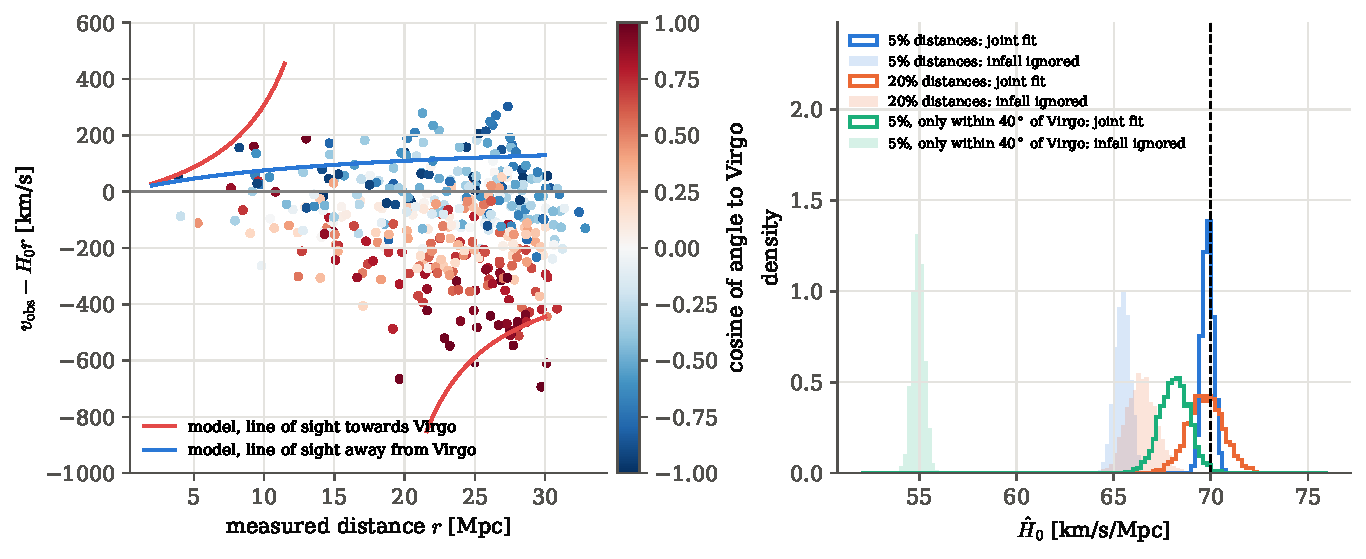
\includegraphics[width=12.5cm]{figures/ch11/virgo_infall.pdf}
\caption{Left: one mock local sample with $5\%$ distances. Each point is a galaxy's
velocity minus the pure Hubble flow, coloured by the cosine of its angle from
Virgo; the curves are the model along the line of sight towards Virgo (red, the
S-shape through the cluster) and away from it (blue, mostly the reflex of our own infall).
Right: $\hat H_0$ over $\FBViNmock$ mock samples, from the joint fit (outlines) and
with the infall ignored (filled), for $5\%$ and $20\%$ distances over the whole sky
and for $5\%$ distances within $40^\circ$ of Virgo. The dashed line is the truth.}
\label{11c:fig:virgo-infall}
\end{figure}

\subsection{Our motion through the CMB}
\label{11c:sec:dipole}

There is one frame in which ``at rest'' has a meaning on cosmological scales: the
frame in which the cosmic microwave background looks the same in every direction.
An observer moving through it with speed $v=\beta c$ sees the radiation ahead
Doppler-shifted to a higher temperature and the radiation behind to a lower one.
To first order in $\beta$ the temperature in a direction at angle $\theta$ to the
motion is $T(\theta)=T_0(1+\beta\cos\theta)$ (see the cosmology notes): a pure dipole
of amplitude $\beta T_0$.

\paragraph{Example: the Sun's speed from the dipole.} Planck measures a dipole
amplitude of $3362.08\,\mu$K and a monopole $T_0=2.7255$\,K \cite[Table~3]{Planck2018I}.
Then $\beta=3362.08\times10^{-6}/2.7255=\FBViBeta\times10^{-3}$, and
$v=\beta c=\FBViVsunCMB$\,km/s, towards Galactic longitude and latitude
$(l,b)=(264.0^\circ,48.3^\circ)$: Planck's $369.82\pm0.11$\,km/s.

The Sun's velocity is the sum of its motion relative to the Local Group and the
Local Group's motion relative to the CMB. The first is measured from the
velocities of the Local Group members, as Hubble's solar motion was from his
nebulae; Planck adopts $299\pm15$\,km/s towards $(98.4^\circ,-5.9^\circ)$
\cite[Table~3]{Planck2018I}. Converting each speed and direction to a vector, with
the unit vector $(\cos b\cos l,\cos b\sin l,\sin b)$, and subtracting,
\[
  \bm v_{\rm LG-CMB}=\bm v_{\rm Sun-CMB}-\bm v_{\rm Sun-LG},
\]
gives $\FBViLGspeed$\,km/s towards $(\FBViLGl^\circ,\FBViLGb^\circ)$, which is Planck's
$620\pm15$\,km/s towards $(271.9^\circ,29.6^\circ)$. The Local Group moves through the
CMB at more than six hundred kilometres per second.

\emph{How much of it is Virgo?} The direction of Virgo is $(283.8^\circ,74.5^\circ)$,
$\FBViLGang^\circ$ from the Local Group's motion, so the component of the motion
towards Virgo is $\FBViLGcomp$\,km/s. An infall of $200$\,km/s accounts for less than
half of that, and subtracting a $200$\,km/s vector pointing at Virgo leaves
$\FBViLGresid$\,km/s pointing elsewhere. That remainder is produced by mass beyond
the Local Supercluster: in the 1980s, the peculiar velocities of elliptical
galaxies revealed a large-scale streaming towards a concentration of mass named
the Great Attractor \cite{LyndenBell1988}, and the slow fall-off of the velocity
correlation $\psi_\perp$ in \cref{11c:fig:pecvel-theory} says that contributions from a
hundred megaparsecs and more are expected. Our own velocity is a sum over the
whole volume, as \eqref{11c:eq:u-integral} says it must be.

\paragraph{The lesson.} The local flow is a field, not a scatter: modelling the
infall into Virgo removes a bias many times larger than the statistical error on
$H_0$, and poor distances bias the infall itself, because the regressor that
describes the flow is evaluated at the wrong place.
\section{How well can a local measurement know \texorpdfstring{$H_0$}{H0}?}
\label{11c:sec:cosmicvar}

Every measurement of $H_0$ from distances and redshifts uses tracers inside some
region around us: Hubble's out to a couple of megaparsecs on his scale, the
supernovae of the modern distance ladder out to $z\approx0.15$, some
$450\,h^{-1}$Mpc. Inside that region the matter density is not exactly the cosmic
mean, and \cref{11c:sec:virgo} showed that a mean contrast inside a sphere changes
the expansion rate seen from its centre. So the ``local $H_0$'' we measure differs
from the global one by an amount that depends on where we happen to live. That
amount is random: had we lived elsewhere, it would be different. Its spread over
all possible observers is the \newterm{cosmic variance} of a local $H_0$. It sets a
floor under every local measurement, no matter how many tracers it uses, and it
decides whether the gap between the ladder and the CMB could be the accident of
living in an underdense region.

\emph{Where we have met $H_0$ before.} The question was first asked in
\cref{T2b:sec:tension}. There the ladder's $73.04\pm1.04$ lay $8.4\%$ above Planck's
$67.36\pm0.54$, and linear continuity, $\delta H_0/H_0=-f\delta/3$, said that a void
explaining it would have to be almost half empty, $|\delta|\approx0.45$, over the whole
volume of the Hubble-flow supernovae, against an expected scatter of $0.5$ to $1\%$
quoted from the literature. The physics here is the same, and so is that relation. What
is new is the statistics: there the void was one sphere of chosen depth, here the
density is a random field drawn from the CAMB spectrum, the same field that moved the
galaxies of \cref{11c:sec:pecvel} and pulled us towards Virgo in \cref{11c:sec:virgo},
and the local $H_0$ is an estimator whose spread over observers we compute rather than
quote. The mock samples of \cref{3b:sec:hubble} and \cref{11c:sec:virgo} asked whether a
fit recovers a known $H_0=70$ from noisy tracers; here even perfect tracers give a
local value that differs from the global one, and the question is by how much. The
required depth comes out as $0.48$ in \cref{11c:sec:tension-void}, not $0.45$, only
because the gap is kept at $8.4\%$ there instead of being rounded to $8\%$.

The sentence ``the cosmic variance of $H_0$ inside a sphere of radius $R$'' sounds
complete, and is not. It hides a choice: the estimator that turns the tracers'
velocities into one number. Two reasonable estimators, applied to
the same tracers in the same sphere, have cosmic variances that differ by $12$ to
$17\%$ at every radius, and two well-known papers quote, in effect, different estimators.

\paragraph{The question.}
\begin{enumerate}
  \item An observer fits $H$ to the radial velocities of tracers inside a sphere of
        radius $R$. By how much does the answer differ from the global $H_0$, as a
        function of the density field?
  \item What is the spread of that difference over observers, for the CAMB
        spectrum, and how does it depend on $R$ and on the estimator?
  \item Do we reproduce the numbers of Wojtak et al.\ (2014) and Marra et al.\ (2013)?
  \item Could it explain the Hubble tension?
\end{enumerate}

\subsection{The estimator decides the window}
\label{11c:sec:window}

\emph{The setup.} We sit at the origin. Tracers fill the sphere $|\bm x|<R$
uniformly and densely. Velocities are measured in the frame of the CMB, so our own
motion is removed (\cref{11c:sec:dipole}), and tracer $i$ at distance $r_i$ has radial
velocity $v_i=H_0r_i+\bm u(\bm x_i)\cdot\hat{\bm r}_i$, with $\bm u$ the linear velocity
field of \cref{11c:sec:pv-linear}. We assume the distances are exact, so that the only
departure from the Hubble law is the flow.

\emph{The least-squares slope.} The estimator of \eqref{11c:eq:k-origin} is
$\hat H=\sum_iv_ir_i/\sum_ir_i^2$. Since $\bm u\cdot\hat{\bm r}\,r=\bm u\cdot\bm x$,
\[
  \hat H-H_0=\frac{\sum_i\bm u(\bm x_i)\cdot\bm x_i}{\sum_ir_i^2}
  \;\longrightarrow\;
  \frac{\int_V\bm u\cdot\bm x\,\dd^3x}{\int_Vr^2\,\dd^3x},
\]
where the arrow is the limit of many tracers with uniform number density: each sum
becomes the density times an integral over the sphere $V$, and the density cancels.

\emph{What could make the numerator nonzero?} Only the divergence of the flow, as
we now show. The product rule gives $\nabla\cdot(r^2\bm u)=r^2\,\nabla\cdot\bm u+2\,\bm u\cdot\bm x$,
since $\nabla r^2=2\bm x$. So
\begin{align}
  \int_V\bm u\cdot\bm x\,\dd^3x
  &\eqby{1}\frac12\Bigl[\oint_{r=R}r^2\,\bm u\cdot\dd\bm S-\int_Vr^2\,\nabla\cdot\bm u\,\dd^3x\Bigr]
   \eqby{2}\frac12\int_V\bigl(R^2-r^2\bigr)\,\nabla\cdot\bm u\,\dd^3x
  \nonumber\\
  &\eqby{3}-\frac{H_0f}{2}\int_V\bigl(R^2-r^2\bigr)\,\delta\,\dd^3x,
  \nonumber\\
  \frac{\hat H-H_0}{H_0}
  &\eqby{4}-\frac{f}{2}\,\frac{5}{4\pi R^5}\int_V\bigl(R^2-r^2\bigr)\,\delta\,\dd^3x
   \eqby{5}-\frac{f}{3}\,\delta_W,
  \qquad
  \delta_W\equiv\int\dd^3x\;W_{\rm LS}(\bm x)\,\delta(\bm x).
  \label{11c:eq:dH-window}
\end{align}
\begin{explain}
  \item Integrate the product rule over $V$ and use the divergence theorem on
        $\nabla\cdot(r^2\bm u)$.
  \item On the surface $r=R$, so $r^2=R^2$ comes out, and
        $\oint\bm u\cdot\dd\bm S=\int_V\nabla\cdot\bm u\,\dd^3x$ by the divergence theorem
        again.
  \item The continuity equation (V1) of \cref{11c:sec:pv-linear} today, $a=1$,
        $H=H_0$.
  \item Divide by $\int_Vr^2\dd^3x=4\pi\int_0^Rr^4\dd r=4\pi R^5/5$ and by $H_0$.
  \item Define the normalised \newterm{window}
        $W_{\rm LS}(\bm x)=\frac{15}{8\pi R^5}(R^2-r^2)$ for $r<R$ and zero outside.
        Its integral is $\frac{15}{8\pi R^5}\,4\pi\bigl(\frac{R^5}{3}-\frac{R^5}{5}\bigr)=1$,
        so $\int_V(R^2-r^2)\delta=\frac{8\pi R^5}{15}\delta_W$, and
        $\frac f2\cdot\frac{5}{4\pi R^5}\cdot\frac{8\pi R^5}{15}=\frac f3$.
\end{explain}

\begin{keyidea}[The local Hubble rate measures a weighted density]
To linear order, a local estimate of $H_0$ is off by
$\delta H/H_0=-\tfrac13 f\,\delta_W$, where $\delta_W$ is the density contrast
averaged with a window set by the estimator. For the least-squares slope through
the origin the window is $\propto R^2-r^2$ inside the sphere: the sphere's centre
counts most.
\end{keyidea}

The surprise is the shape. One might have guessed that the least-squares slope,
which weights each tracer by $r_i^2$ and so favours the distant ones, measures the
density near the edge. It measures the opposite. A tracer at the edge feels the
mass inside it; a tracer near the centre feels the mass inside its own smaller
sphere; the mass near the centre is felt by every tracer, so it accumulates the
largest weight.

\emph{Other estimators, other windows.} Averaging the individual ratios
$v_i/r_i$, the \newterm{mean of ratios} $\hat H=N^{-1}\sum_iv_i/r_i$, goes the same way
with $\bm u\cdot\bm x/r^2=\bm u\cdot\nabla\ln r$ in place of $\bm u\cdot\bm x$, and the
product rule for $\nabla\cdot(\bm u\ln r)$ gives the window
$W_{\rm MR}=\frac{9}{4\pi R^3}\ln(R/r)$, even more concentrated at the centre (it
diverges there, slowly). And if all tracers sat on the surface $r=R$, the slope
would be $u_R(R)/R$, which by \eqref{11c:eq:infall} is $-\tfrac13H_0f\,\bar\delta(<R)$: the
mean contrast inside the sphere, a uniform \newterm{top-hat} window
$W_{\rm TH}=3/(4\pi R^3)$. This is the ``Hubble bubble'' of Marra et al.\ and the
local-void example of \cref{T2b:sec:ladder}. All three share the same
$-\tfrac13f$; they differ only in the window (\cref{11c:fig:windows}, left).

\subsection{From the window to the variance}
\label{11c:sec:window-variance}

The contrast $\delta_W$ is a linear functional of a Gaussian field, so it is
Gaussian with mean zero and variance
$\langle\delta_W^2\rangle=\int\frac{\dd^3k}{(2\pi)^3}P(k)\,|\tilde W(\bm k)|^2$, where
$\tilde W$ is the Fourier transform of the window (\cref{7a:sec:smoothing}, where
the same step gave $\sigma_8$). For a spherical window
$\tilde W(k)=4\pi\int_0^RW(r)\,r^2j_0(kr)\,\dd r$, the angular integral being the one
that gave $j_0$ in \cref{11c:sec:pv-corr}. So
\begin{equation}
  \sigma^2\!\Bigl(\frac{\delta H}{H_0}\Bigr)=\Bigl(\frac f3\Bigr)^2\frac{1}{2\pi^2}
  \int_0^\infty\dd k\;k^2P(k)\,\tilde W^2(kR).
  \label{11c:eq:sigma-H}
\end{equation}

\emph{The transform of the parabolic window.} We need one identity for spherical
Bessel functions, $\frac{\dd}{\dd x}\bigl[x^{n+1}j_{n+1}(x)\bigr]=x^{n+1}j_n(x)$. For
$n=0$: $x^2j_1=\sin x-x\cos x$, whose derivative is $x\sin x=x^2j_0$. For $n=1$:
$x^3j_2=(3-x^2)\sin x-3x\cos x$, whose derivative is
$-2x\sin x+(3-x^2)\cos x-3\cos x+3x\sin x=x\sin x-x^2\cos x=x^3j_1$. With $x=kr$,
$X=kR$,
\begin{align}
  \int_0^R\bigl(R^2-r^2\bigr)r^2j_0(kr)\,\dd r
  &\eqby{1}\frac{1}{k^5}\int_0^X\bigl(X^2-x^2\bigr)x^2j_0(x)\,\dd x
  \nonumber\\
  &\eqby{2}\frac{1}{k^5}\Bigl[X^2\cdot X^2j_1(X)-\Bigl(X^4j_1(X)-2\!\int_0^X\!x^3j_1(x)\,\dd x\Bigr)\Bigr]
  \nonumber\\
  &\eqby{3}\frac{2X^3j_2(X)}{k^5},
  \nonumber\\
  \tilde W_{\rm LS}(kR)
  &\eqby{4}4\pi\,\frac{15}{8\pi R^5}\,\frac{2X^3j_2(X)}{k^5}=\frac{15\,j_2(kR)}{(kR)^2}.
  \label{11c:eq:W-LS}
\end{align}
\begin{explain}
  \item Substitute $r=x/k$: $R^2-r^2=(X^2-x^2)/k^2$ and $r^2\dd r=x^2\dd x/k^3$.
  \item The first term is the $n=0$ identity integrated. For the second, integrate
        $x^2\cdot x^2j_0$ by parts, with $x^2j_1$ as the antiderivative of $x^2j_0$.
  \item The $X^4j_1$ terms cancel, and the $n=1$ identity integrates $x^3j_1$ to $X^3j_2$.
  \item Multiply by $4\pi$ and the normalisation of $W_{\rm LS}$; $X^3/(R^5k^5)=1/X^2$.
\end{explain}
A check: for small $X$, $j_2(X)\approx X^2/15$, so $\tilde W_{\rm LS}\to1$, as a normalised
window must. The same steps give $\tilde W_{\rm TH}=3j_1(kR)/(kR)$ (only the $n=0$
identity) and, integrating $\ln(R/r)$ by parts, $\tilde W_{\rm MR}=9\bigl[\mathrm{Si}(kR)-\sin kR\bigr]/(kR)^3$,
with $\mathrm{Si}$ the sine integral. \Cref{11c:fig:windows} (right) shows that the
more a window concentrates at the centre, the further out in $k$ its transform
reaches, and the more small-scale power it lets into the variance.

\begin{figure}[htbp]
\centering
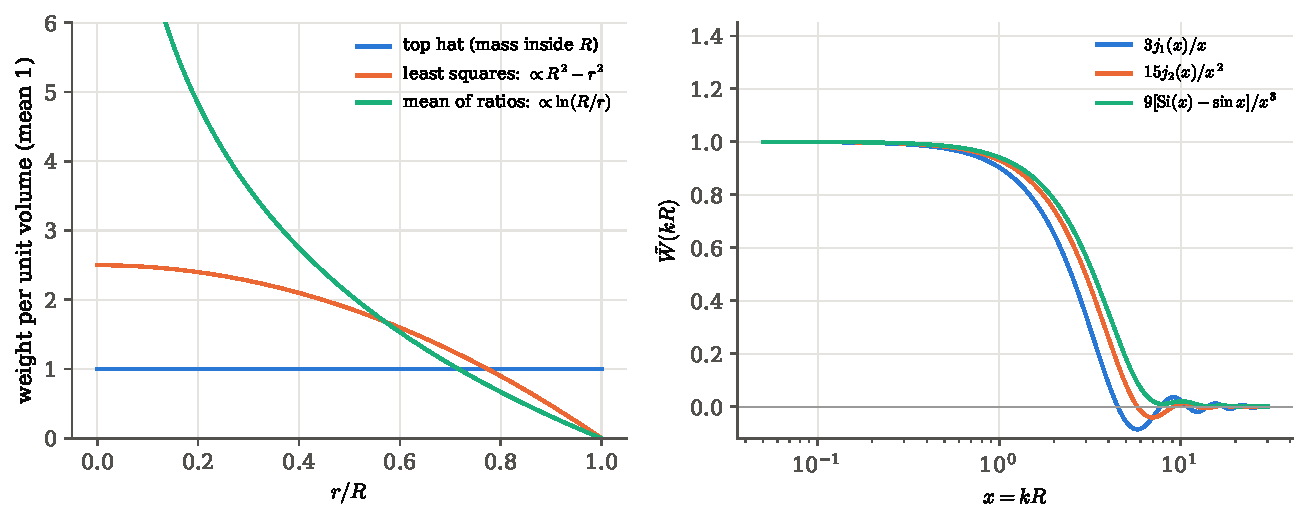
\includegraphics[width=12.5cm]{figures/ch11/local_h0_windows.pdf}
\caption{The three windows. Left: the weight each estimator gives to the density at
radius $r$ inside the sphere, normalised to unit mean over the volume. Right: their
Fourier transforms. The parabolic window of the least-squares slope reaches higher
$k$ than the top hat, and the logarithmic window of the mean of ratios higher still.}
\label{11c:fig:windows}
\end{figure}

\paragraph{Example: the numbers.} Script \pyname{code/ch11/11_local_h0_variance.py}
evaluates \eqref{11c:eq:sigma-H} with the CAMB spectrum and $f=\FBLhF$. At
$R=50\,h^{-1}$Mpc the rms of $\delta H/H_0$ is $\FBLhTHFifty\%$ for the top hat,
$\FBLhLSFifty\%$ for the least-squares slope and $\FBLhMRFifty\%$ for the mean of ratios;
at $100\,h^{-1}$Mpc, $\FBLhTHHund$, $\FBLhLSHund$ and $\FBLhMRHund\%$. The least-squares
value falls to $\FBLhLSOneFifty\%$ at $150$ and $\FBLhLSThreeHund\%$ at $300\,h^{-1}$Mpc,
roughly as $R^{-1.5}$ (\cref{11c:fig:local-h0}, left). A percent-level local $H_0$
needs tracers out to at least $100\,h^{-1}$Mpc.

\subsection{Checking the window on Gaussian boxes}
\label{11c:sec:window-box}

The derivation used two idealisations: a continuum of tracers and the linear
velocity field. The second we cannot test with a Gaussian simulation, but the
first, and all the algebra, we can. The script draws four Gaussian boxes of side
$\FBLhBoxL\,h^{-1}$Mpc with $\FBLhBoxN^3$ cells, computes the velocity field as in
\cref{11c:sec:pv-box}, places $\FBLhNobs$ observers at random, and lets each fit the
least-squares slope to $\FBLhNpts$ tracers inside spheres of five radii.

\pyfile[firstline=133,lastline=144,firstnumber=133]{code/ch11/11_local_h0_variance.py}{Observers at random positions fit $H$ to tracers inside a sphere}

\noindent Lines 136--140 draw tracers uniformly in the volume of the sphere: the
radius as $R\,U^{1/3}$, so that the number within $r$ grows as $r^3$, and an
isotropic direction. Line 142 finds the cell of each tracer, line 143 takes the
radial velocity there, and line 144 is the least-squares slope, divided by
$100$\,km/s per $h^{-1}$Mpc to give $\delta H/H_0$.

The rms over observers is $\FBLhBoxFifty$, $\FBLhBoxHund$, $\FBLhBoxOneFifty$,
$\FBLhBoxTwoHund$ and $\FBLhBoxThreeHund\%$ at $R=50$, $100$, $150$, $200$, $300\,h^{-1}$Mpc,
against $\FBLhGridFifty$, $\FBLhGridHund$, $\FBLhGridOneFifty$, $\FBLhGridTwoHund$ and
$\FBLhGridThreeHund\%$ from \eqref{11c:eq:sigma-H} summed over the box's modes. The
simulation agrees with the prediction to within a few per cent, about what four
boxes allow: the observers in one box share its long waves and
are far from independent, so the effective number of independent samples is much
smaller than $\FBLhNobs$. The mean of $\delta H/H_0$ is zero within that scatter: its
largest value, $\FBLhBoxMeanFifty\%$ at $R=50\,h^{-1}$Mpc, is a small fraction of the
$\FBLhBoxFifty\%$ rms there.

\begin{figure}[htbp]
\centering
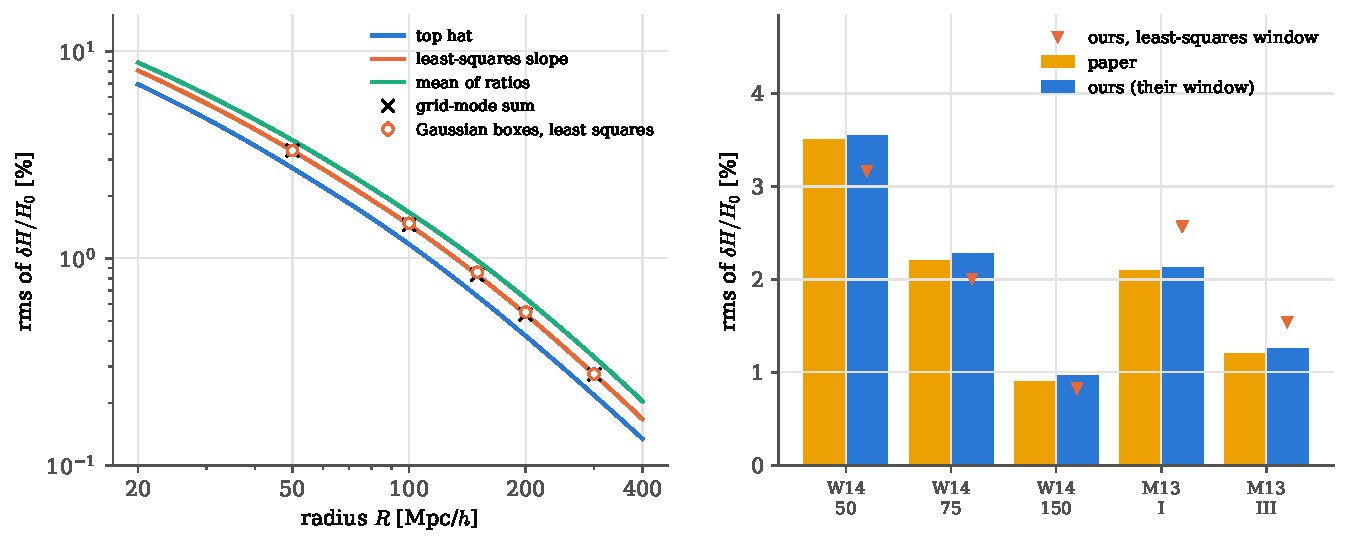
\includegraphics[width=12.5cm]{figures/ch11/local_h0_sigma.pdf}
\caption{Left: the rms deviation of a local Hubble constant from the global one,
for the three windows, with the least-squares estimator measured on Gaussian boxes
(circles) and the grid-mode sum (crosses). Right: our reproduction of Wojtak et
al.\ (2014) at three radii and of Marra et al.\ (2013), cases I and III. Orange
bars: the paper; blue bars: our calculation with the paper's window; triangles: the
same calculation with the least-squares window.}
\label{11c:fig:local-h0}
\end{figure}

\subsection{Reproduction: Wojtak et al.\ (2014)}
\label{11c:sec:wojtak}

\emph{Their question.} By 2013 the supernova measurement of $H_0$ had a $3\%$ error
and differed from Planck's by $2.4\sigma$. Wojtak and collaborators asked how large
the scatter of a local $H_0$ is in a realistic simulated universe, and how much it
depends on where the observers sit: at random points, in dark-matter haloes like
the one we live in, or in the centres of voids \cite{Wojtak2014}.

\emph{Their setup.} An $N$-body simulation of a $(6\,h^{-1}\mathrm{Gpc})^3$ box in a WMAP-like
cosmology ($\Omega_m=0.27$, $\Omega_b=0.044$, $h=0.70$, $\sigma_8=0.80$, $n_s=0.96$),
with haloes identified in it. For each of $10^5$ observers they fit their eq.~(1),
$\bm u\cdot\hat{\bm r}+H_0r=H_{\rm loc}r$, to all haloes within $r_{\max}$, with equal
weights. Their Table~1 gives the scatter of $H_{\rm loc}/H_0-1$ at $r_{\max}=50$, $75$
and $150\,h^{-1}$Mpc, from the simulation and from a linear-theory formula, their
eq.~(3), with $f=\Omega_m^{0.55}$.

\emph{Their equation, derived.} Their eq.~(3) reads, in our notation,
\[
  \sigma^2\!\Bigl(\frac{\delta H}{H_0}\Bigr)=\frac{f^2}{2\pi^2R^2}\int_0^\infty\dd k\,P(k)
  \Bigl[\frac{3(\sin x-\mathrm{Si}\,x)}{x^2}\Bigr]^2,\qquad x=kR .
\]
This is \eqref{11c:eq:sigma-H} with the mean-of-ratios window:
\begin{align*}
  \Bigl(\frac f3\Bigr)^2\frac{1}{2\pi^2}\int\dd k\,k^2P\,\tilde W_{\rm MR}^2
  &\eqby{1}\frac{f^2}{9}\,\frac{1}{2\pi^2}\int\dd k\,k^2P\,\frac{81(\mathrm{Si}\,x-\sin x)^2}{x^6}
   \eqby{2}\frac{f^2}{2\pi^2R^2}\int\dd k\,P\,\frac{9(\sin x-\mathrm{Si}\,x)^2}{x^4}.
\end{align*}
\begin{explain}
  \item Insert $\tilde W_{\rm MR}=9(\mathrm{Si}\,x-\sin x)/x^3$.
  \item $k^2/x^6=1/(R^2x^4)$ since $x=kR$; $81/9=9$; the square removes the sign.
\end{explain}
So the formula they quote describes averaging the ratios $u_r/r$; the fit they ran on
the haloes was the least-squares slope, whose window is the parabola.

\emph{What we compute.} The CAMB linear spectrum for their cosmology, normalised to
$\sigma_8=0.80$, and \eqref{11c:eq:sigma-H} with both windows and $f=0.27^{0.55}=\FBLhWf$.

\emph{Side by side.}
\begin{center}
\small
\begin{tabular}{@{}lccc@{}}
\toprule
$r_{\max}$ [$h^{-1}$Mpc] & $50$ & $75$ & $150$\\
\midrule
Wojtak et al., linear theory (their eq.~3) & $3.5\%$ & $2.2\%$ & $0.9\%$\\
ours, same formula (mean-of-ratios window) & $\FBLhWMRa\%$ & $\FBLhWMRb\%$ & $\FBLhWMRc\%$\\
ours, least-squares window & $\FBLhWLSa\%$ & $\FBLhWLSb\%$ & $\FBLhWLSc\%$\\
Wojtak et al., simulation, observers at random points & $3.3\%$ & $2.1\%$ & $0.9\%$\\
\bottomrule
\end{tabular}
\end{center}

\emph{Why they differ.} Our evaluation of their formula agrees with their linear
row to within the last digit they quote; the remaining few per cent are what a
different transfer function or a rounding of their table would produce. The
least-squares window, which is the estimator actually applied to their haloes,
gives values $11$--$14\%$ lower. Their simulation lies between the two: at
$150\,h^{-1}$Mpc, where linear theory should be good, it is $0.9\%$ against our $0.83\%$;
at $50\,h^{-1}$Mpc non-linear growth adds variance, and the authors note that voids,
which fill most of the volume, push the mean of $H_{\rm loc}$ above $H_0$ there.

\emph{The lesson.} ``The cosmic variance of $H_0$ within $R$'' is a property of an
estimator, not of the sphere: the same tracers give a $12$--$17\%$ larger scatter when
their ratios are averaged than when a slope is fitted, because the two weight the
density near us differently.

\subsection{Reproduction: Marra et al.\ (2013)}
\label{11c:sec:marra}

\emph{Their question.} In 2013 the local value was $73.8\pm2.4$\,km/s/Mpc and the first
Planck release gave $67.8\pm0.8$, a gap of
$(73.8-67.8)/\sqrt{2.4^2+0.8^2}=6.0/2.53=2.4$ standard deviations (the variance of a
difference of independent measurements is the sum of the variances). Today's values,
$73.04\pm1.04$ and Planck's final $67.36\pm0.54$, leave a gap of about the same size in
km/s/Mpc but a much smaller error, so the same gap is $4.8$ standard deviations
(\cref{11c:sec:h0-routes}). How much of it can the local
gravitational potential absorb, and what systematic error should every local
measurement carry for it \cite{Marra2013}?

\emph{Their setup.} A Hubble bubble: a top hat, so that their eq.~(1) is
$\delta H/H=-\tfrac13f\,\delta$ (in the linear regime, where their non-linear
correction $\Theta$ equals one), which is \eqref{11c:eq:infall}. The contrast inside a
sphere of radius $R$ is Gaussian with the top-hat variance $\sigma_R^2$ (their
eqs.~2--3). The supernovae lie at redshifts between $z_{\min}$ and $0.1$, and each
redshift $z$ is assigned the sphere of comoving radius $R(z)$. The resulting
variances are averaged over the redshift distribution $W_{\rm SN}(z)$ of the
supernovae:
\[
  \sigma_{H_0}^2=\int_{z_{\min}}^{z_{\max}}\dd z\;W_{\rm SN}(z)\,
  \Bigl(\frac f3\Bigr)^2\sigma_{R(z)}^2 \qquad\text{(their eq.~5)}.
\]
Their Table~I gives $2.1\%$ for $z_{\min}=0.010$ (case~I) and $1.2\%$ for
$z_{\min}=0.023$ (case~III).

\emph{Their equation, derived.} $\sigma_{R}^2$ is \eqref{11c:eq:sigma-H} without the
$(f/3)^2$ and with $\tilde W_{\rm TH}$; eq.~(5) is the variance of $\delta H/H$ averaged
over the redshifts of the supernovae, each probing the sphere out to its own
distance.

\emph{What we compute.} The one input not given in the paper is $W_{\rm SN}(z)$. They
state its medians: $0.025$ for $z_{\min}=0.010$ and $0.033$ for $z_{\min}=0.023$. A
lognormal distribution in $z$, truncated to $[z_{\min},0.1]$, has two parameters, and
the two medians fix them: median $\FBLhMuz$ and logarithmic width $\FBLhSz$ before
truncation. We use the Planck 2018 spectrum rather than their Planck 2013 one; the
matter densities differ by $2\%$.

\emph{Side by side.} Case~I: $\FBLhMone\%$ against their $2.1\%$. Case~III:
$\FBLhMthree\%$ against $1.2\%$. With the least-squares window instead of the top hat
the same averages would be $\FBLhMoneLS\%$ and $\FBLhMthreeLS\%$.

\emph{Why they differ.} At the quoted precision they do not; our $W_{\rm SN}$ is a
reconstruction, and a different shape with the same medians would move the
results by a few hundredths of a per cent.

\emph{The lesson.} A two-line linear-theory calculation, with the supernova
distribution rebuilt from two quoted medians, reproduces the published systematic
floor; the floor is about $1\%$ once the nearest supernovae are excluded.

\begin{inpractice}
The Gaussian boxes \emph{verify} \eqref{11c:eq:sigma-H}: they check an analytic result
in the regime where it should hold exactly. Wojtak et al.'s $N$-body simulation is
the \emph{research instrument}. It answers what no formula can: the scatter when
observers live in haloes rather than at random points (lower $H_{\rm loc}$, because
haloes sit in infall regions), when velocities are measured relative to the halo
rather than the CMB, and when non-linear voids dominate the small spheres. The same
division of labour runs through the book: closed forms where they exist, checked by
simulation; simulation alone where they do not (\cref{ch:06}).
\end{inpractice}

\subsection{Could we live in a hole?}
\label{11c:sec:tension-void}

The ladder value $73.04$ exceeds Planck's $67.36$ by $\FBLhGap\%$. To produce that by
\eqref{11c:eq:dH-window}, the density averaged over the ladder's window would need
$\delta_W=-3\times0.084/f=\FBLhDeltaW$: a region half empty out to hundreds of
megaparsecs, as \cref{T2b:sec:ladder} estimated. How unlikely is that? The ladder uses
supernovae between $z=0.023$ and $0.15$. With Marra's distribution extended to
$z_{\max}=0.15$, the averaged scatter is $\FBLhShoes\%$ for the top hat and
$\FBLhShoesLS\%$ for the least-squares window, so the gap is $\FBLhNsig$ standard
deviations of the larger one. For a Gaussian, a fluctuation of more than five
standard deviations in one direction has probability below $3\times10^{-7}$. A lognormal density field makes deep
voids somewhat more probable than a Gaussian, as Marra et al.\ show, and observers
at the centres of the ten largest voids in Wojtak et al.'s simulation see
$H_{\rm loc}$ about $5\%$ high out to $100\,h^{-1}$Mpc, falling to $1\%$ at $200\,h^{-1}$Mpc; but at the ladder's distances both effects fall far
short. Cosmic variance is a real systematic error of order $1\%$ and should be in
every local error budget \cite[Sec.~IV.F]{Abdalla2022}; it is not the explanation of
the Hubble tension.
\section{Where is a galaxy whose distance we measured? Malmquist bias}
\label{11c:sec:ihm}

A distance indicator such as the Tully--Fisher relation is calibrated so that it is
right on average: take many galaxies at the same true distance $r$, measure them,
and the logarithms of their inferred distances average to $\ln r$. The plain claim
that follows seems harmless: \emph{an unbiased indicator gives unbiased distances.}
The everyday question it answers is: \emph{if I take all the galaxies that my
indicator places at distance $d$, are they on average at distance $d$?}

The question contains a hidden assumption. ``Unbiased'' was established by
averaging over galaxies at a fixed \emph{true} distance. The question averages over
galaxies at a fixed \emph{inferred} distance. Those are two different sampling
rules, and they select two different sets of galaxies. The galaxies that end up
labelled $d$ came from a range of true distances, and how many came from each
depends on how many galaxies there were at each true distance to begin with. In a
uniform universe there are more galaxies at larger distances, simply because a
shell of larger radius has more volume, so more of them scatter \emph{in} to $d$ from
beyond than from in front. Near a cluster, where the number of galaxies changes
rapidly along the line of sight, the effect is larger and changes sign from one side
of the cluster to the other. Read as peculiar velocities, the mislabelled distances
produce flows that do not exist. We met the first sign of this in
\cref{11c:sec:infall-sim}, where poor distances weakened the fitted infall towards
Virgo.

This is the \newterm{inhomogeneous Malmquist bias}. It is a cousin of the classical
Malmquist bias of \cref{T2b:sec:malmquist}, where a flux limit selected the
unusually bright objects; here no selection is needed at all.

\paragraph{The question.}
\begin{enumerate}
  \item Given an inferred distance $d$, what is the probability distribution of the
        true distance $r$?
  \item What is the mean true distance $E(r\given d)$ in a uniform universe, and near a
        density gradient?
  \item Does a simulated line of sight through a cluster reproduce the bias found by
        Strauss and Willick?
  \item What does the bias do to inferred peculiar velocities, and how should a
        peculiar velocity be estimated from a lognormal distance?
\end{enumerate}

\subsection{The distribution of the true distance}
\label{11c:sec:ihm-bayes}

\emph{Inputs.}
\begin{enumerate}[label=(M\arabic*),leftmargin=2.6em,itemsep=1pt]
  \item \emph{Physical: lognormal errors.} For a galaxy at true distance $r$, the
        inferred distance is $d=re^{\Delta\eta}$ with $\eta\sim\Normal(0,1)$. A magnitude
        error $\sigma$ in a distance modulus is a fractional distance error
        $\Delta=(\ln10/5)\sigma\approx0.46\sigma$, so $0.35$\,mag gives $\Delta=\FBMbDelta$.
  \item \emph{Physical: galaxies along the line of sight.} In a narrow cone around
        the line of sight, the number of galaxies between $r$ and $r+\dd r$ is
        proportional to $r^2n(r)\,\dd r$, with $n(r)$ their number density.
  \item \emph{Selection does not depend on the true distance.} Galaxies enter the
        sample through observed quantities (an apparent size, a line width) whose
        selection is the same at every true distance. Strauss and Willick show that
        the selection then cancels from what follows \cite[Sec.~6.5.2]{StraussWillick1995};
        when it does not, the classical Malmquist bias of \cref{T2b:sec:malmquist}
        appears on top.
\end{enumerate}

\emph{The event.} Our indicator says ``$d$''. \emph{What could have produced it?}
Any true distance $r$: a galaxy at $r$ produces the label $d$ if its error happened
to be $\eta=\ln(d/r)/\Delta$. \emph{How probable was the label under each candidate?}
By (M1), the density of $d$ given $r$ is lognormal,
$p(d\given r)=\exp\bigl[-\ln^2(d/r)/2\Delta^2\bigr]/(\sqrt{2\pi}\,\Delta\,d)$. \emph{Only
then the prior}: how many galaxies were at $r$ to begin with, $r^2n(r)$ by (M2). Bayes'
theorem \eqref{5a:eq:bayes} puts them together:
\begin{equation}
  p(r\given d)=\frac{r^2n(r)\,\exp\bigl[-\ln^2(r/d)/2\Delta^2\bigr]}
                    {\int_0^\infty\dd r'\,r'^2n(r')\,\exp\bigl[-\ln^2(r'/d)/2\Delta^2\bigr]},
  \qquad
  E(r\given d)=\int_0^\infty r\,p(r\given d)\,\dd r .
  \label{11c:eq:ihm-exact}
\end{equation}
The factor $1/d$ and the constants of the lognormal cancel between numerator and
denominator, and the square of $\ln(d/r)$ equals that of $\ln(r/d)$. This is
eq.~(182) of Strauss and Willick, and the mean is their eq.~(183). It depends on the
density all along the line of sight, wherever the lognormal reaches: the bias at $d$
is not a local property of the point $d$.

\begin{figure}[htbp]
\centering
\begin{tikzpicture}[scale=0.95]
  \draw[->] (0,0) -- (6.6,0) node[anchor=north west,font=\small] {true $r$};
  \draw[->] (0,0) -- (0,6.0) node[anchor=south east,font=\small] {inferred $d$};
  \fill[formblue!10] (0,0) -- (4.44,6.0) -- (6.5,6.0) -- (6.5,4.82) -- cycle;
  \draw[formblue!60] (0,0) -- (4.44,6.0);
  \draw[formblue!60] (0,0) -- (6.5,4.82);
  \draw[faint,dashed] (0,0) -- (6.0,6.0);
  \fill[bdryred!18] (3.2,0) rectangle (3.8,6.0);
  \node[anchor=north,font=\small,bdryred!80!black] at (3.5,-0.05) {cluster};
  \draw[thick,fibreorange] (2.22,3.0) -- (4.05,3.0);
  \node[anchor=east,font=\small,fibreorange!80!black] at (-0.05,3.0) {$d$};
  \draw[faint] (0,3.0) -- (2.22,3.0);
  \fill[black] (3.0,3.0) circle (1.8pt);
  \fill[bdryred] (3.38,3.0) circle (2.2pt);
  \node[anchor=south east,font=\small] at (2.95,3.05) {$r=d$};
  \node[anchor=north west,font=\small,bdryred!80!black] at (4.1,2.95) {$E(r\given d)$};
  \draw[faint] (3.42,2.98) -- (4.12,2.75);
\end{tikzpicture}
\caption{Conditioning on the inferred distance. Galaxies at true distance $r$ are
scattered vertically into the blue band of inferred distances. Fixing the label $d$
keeps only the horizontal orange segment: the galaxies that could have produced
that label. Where the segment crosses the cluster (red strip), there are many more
galaxies than elsewhere, so the mean true distance of the galaxies labelled $d$ is
pulled towards the cluster.}
\label{11c:fig:ihm-cartoon}
\end{figure}

\subsection{A uniform universe, and a slowly varying one}
\label{11c:sec:ihm-uniform}

\emph{Uniform density.} Let $n$ be constant and change variable to $y=\ln r$, so
$\dd r=r\,\dd y$ and the prior $r^2\dd r$ becomes $r^3\dd y=e^{3y}\dd y$. Then
\begin{align}
  p(y\given d)
  &\eqby{1}\propto e^{3y}\exp\Bigl[-\frac{(y-\ln d)^2}{2\Delta^2}\Bigr]
   \eqby{2}\propto\exp\Bigl[-\frac{\bigl(y-\ln d-3\Delta^2\bigr)^2}{2\Delta^2}\Bigr],
  \nonumber\\
  E(r\given d)
  &\eqby{3}E\bigl(e^y\given d\bigr)
   \eqby{4}\exp\Bigl(\ln d+3\Delta^2+\frac{\Delta^2}{2}\Bigr)=d\,e^{7\Delta^2/2}.
  \label{11c:eq:ihm-uniform}
\end{align}
\begin{explain}
  \item \eqref{11c:eq:ihm-exact} with $n$ constant, written in $y$; $\ln(r/d)=y-\ln d$.
  \item Complete the square:
        $3y-\frac{(y-\ln d)^2}{2\Delta^2}=-\frac{(y-\ln d-3\Delta^2)^2}{2\Delta^2}+\text{const}$.
        So $y$ is Gaussian with mean $\ln d+3\Delta^2$ and variance $\Delta^2$.
  \item $r=e^y$.
  \item For a Gaussian $y$ with mean $m$ and variance $s^2$,
        $E(e^y)=e^{m+s^2/2}$, the lognormal mean of \eqref{3b:eq:lognormal-mgf}.
\end{explain}
This is eq.~(184) of Strauss and Willick, first derived for galaxy distances by
Lynden-Bell et al.\ \cite{LyndenBell1988}. For $\Delta=\FBMbDelta$ the factor is
$\FBMbUniFac$: galaxies labelled $d$ are on average $\FBMbUniPct\%$ farther away. Of the
$7/2$, three halves come from the volume factor and one half from the asymmetry of
the lognormal.

\emph{A slowly varying density.} If $n$ changes little over the width of the
lognormal, approximate it near $r=d$ by a power law, $n(r)\approx n(d)(r/d)^{\gamma}$,
with the local logarithmic slope $\gamma(d)=\dd\ln n/\dd\ln r$ at $r=d$. The prior
becomes $e^{(3+\gamma)y}$, the same chain runs with $3$ replaced by $3+\gamma$, and
\begin{equation}
  E(r\given d)\approx d\,e^{(7/2+\gamma)\Delta^2}\approx d\Bigl[1+\Bigl(\frac72+\gamma(d)\Bigr)\Delta^2\Bigr],
  \label{11c:eq:ihm-slow}
\end{equation}
the second form for small $\Delta^2$: Strauss and Willick's eq.~(185). In front of a
cluster the density rises with distance, $\gamma>0$, and the bias is larger; behind
it, $\gamma<0$, and the bias is reduced or reversed.

\emph{When the approximation fails.} A power law must hold across the whole
lognormal, from $de^{-\Delta}$ to $de^{\Delta}$, about $\pm16\%$ of $d$. A cluster of
width $500$\,km/s at $5000$\,km/s varies over $10\%$ of its distance, and its
$|\gamma|$ reaches $\FBMbGammaMax$: \eqref{11c:eq:ihm-slow} then predicts corrections of
order $\gamma\Delta^2\approx0.5$, absurdly large, and the full integral is needed.

\subsection{Reproduction: Strauss and Willick's line of sight through a cluster}
\label{11c:sec:sw-repro}

\emph{Their question.} How large is the Malmquist bias near a realistic density
peak, how good is the slowly varying approximation, and does the exact formula
\eqref{11c:eq:ihm-exact} predict it? \cite[Sec.~6.5.2, Fig.~15]{StraussWillick1995}

\emph{Their setup.} One line of sight. A uniform background density plus a Gaussian
peak centred at $5000$\,km/s (distances in velocity units, $H_0r$), of full width about
$1200$\,km/s and maximum contrast $25$. Galaxies follow pure Hubble flow: no true
peculiar velocities at all. Distances come from a Tully--Fisher relation with
$0.35$\,mag of scatter. They bin the galaxies in $150$\,km/s bins of inferred distance
and plot the mean true distance in each bin.

\emph{Their equations.} \eqref{11c:eq:ihm-exact}, \eqref{11c:eq:ihm-uniform} and
\eqref{11c:eq:ihm-slow}, derived above, are their eqs.~(183)--(185).

\emph{What we compute.} We read ``full width'' as the full width at half maximum,
which gives a Gaussian of standard deviation $\FBMbSp$\,km/s, and draw true
distances with density $\propto r^2n(r)$ so that the peak holds about $800$
galaxies per $200$\,km/s bin, as in their upper panel; that makes $\FBMbN$ galaxies in
all. Each is given $d=re^{\Delta\eta}$. The exact curve is \eqref{11c:eq:ihm-exact}
integrated numerically:

\pyfile[firstline=45,lastline=52,firstnumber=45]{code/ch11/12_malmquist.py}{The exact mean true distance at given inferred distance}

\noindent Line 49 is the lognormal $p(d\given r)$ on a grid of true distances, line 50
multiplies by the number of galaxies at each $r$, and line 51 takes the ratio of the
first moment to the normalisation.

\emph{Side by side.} \Cref{11c:fig:malmquist} has the two panels of their figure,
with a third added. The simulated bins follow the exact curve: over the
$\FBMbNbins$ bins with at least five galaxies, $\chi^2=\FBMbChi$, where a correct curve
gives $\FBMbNbins\pm\FBMbChiSd$. Some realisations give a value on the high side, and
that is expected: each error bar is itself estimated from the few galaxies in its bin, and an error bar that comes out
too small adds a lot to $\chi^2$. Far from the peak
they follow the uniform-density line $de^{7\Delta^2/2}$. In front of the peak,
galaxies scattered out of the cluster pile up at smaller inferred distances, so
the mean true distance at given $d$ is too large; the excess over the uniform
prediction reaches $\FBMbForeV$\,km/s at $d\approx\FBMbForeD$. Behind the peak the sign
reverses, $\FBMbBackV$\,km/s at $d\approx\FBMbBackD$. The slowly varying approximation
oscillates wildly in between, exactly as theirs does. In their figure the
amplitude of the effect is ``$500$--$1000$\,km/s''; ours is in that range in front
and slightly larger behind.

\emph{Why they differ.} Three things are not specified exactly: the width (we
assumed FWHM), the number of background galaxies (their sample had a diameter
limit, which thins the far background and so their high-$d$ bins), and the scatter
of a single realisation. None changes the shape: an S-shaped departure from the
uniform-density line, centred on the peak.

\begin{figure}[htbp]
\centering
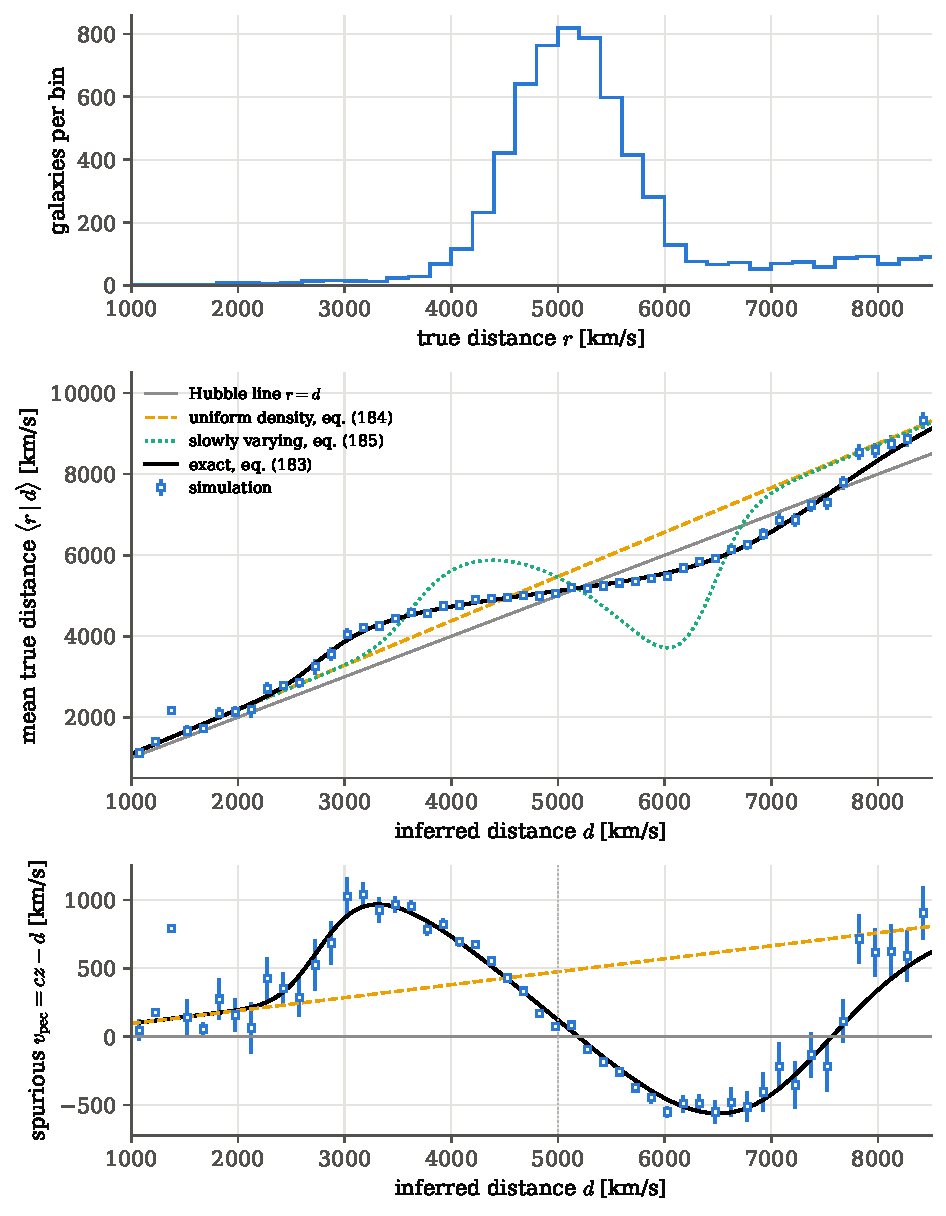
\includegraphics[width=8.6cm]{figures/ch11/malmquist.pdf}
\caption{A line of sight through a density peak, after Strauss and Willick's Fig.~15.
Top: the number of galaxies per $200$\,km/s bin of true distance. Middle: the mean
true distance in $150$\,km/s bins of inferred distance (squares), with the Hubble line
$r=d$, the uniform-density bias, the slowly varying approximation and the exact
integral. Bottom: the same as an apparent peculiar velocity $cz-d$ for galaxies that
in truth have none; the dotted line marks the peak.}
\label{11c:fig:malmquist}
\end{figure}

\paragraph{The spurious flow.} The galaxies have no peculiar velocities. An
observer who takes the inferred distance at face value computes
$v_{\rm pec}=cz-H_0d=H_0(r-d)$, and the bottom panel shows what they find: galaxies in
front of the peak appear to recede faster than the Hubble flow, galaxies behind it
appear to approach. That is exactly the signature of infall onto a mass
concentration, the S-shape of \cref{11c:fig:virgo-infall}, and its amplitude,
hundreds of km/s, is that of a real infall. Uncorrected, the bias makes a peak look
more massive than it is, and inflates the infall it is meant to measure. Every
velocity analysis must either correct the distances with \eqref{11c:eq:ihm-exact},
which needs the density field along each line of sight, or work in redshift space,
where the flow is modelled and the distances are the noisy data.

\paragraph{The lesson.} An indicator that is unbiased at fixed true distance is
biased at fixed inferred distance, because conditioning on what we measured
reweights the possible true distances by how many galaxies were there.

\subsection{A peculiar velocity from a lognormal distance}
\label{11c:sec:log-estimator}

There is a second, smaller trap in $v_{\rm pec}=cz-H_0d$, even for one galaxy at a known
true distance. Take a galaxy in pure Hubble flow at $r$, so $cz=H_0r$. Then
$v_{\rm pec}=H_0r\bigl(1-e^{\Delta\eta}\bigr)$, a nonlinear function of the Gaussian $\eta$. Its
mean is $H_0r\bigl(1-e^{\Delta^2/2}\bigr)<0$ and its distribution has a long tail to
negative values: at $r=5000$\,km/s the mean is $\FBMbMeanNaive$\,km/s and the skewness
$\FBMbSkewNaive$. The fix is to estimate the velocity from the logarithm,
\[
  \hat v_{\rm pec}=cz\,\ln\frac{cz}{H_0d}
  \;=\;H_0r\,\ln\frac{r}{d}=-H_0r\,\Delta\eta ,
\]
which is linear in $\eta$: Gaussian, with mean zero (our simulation gives
$\FBMbMeanLog$\,km/s and skewness $\FBMbSkewLog$). For small velocities it agrees with
$cz-H_0d$ to first order, since $\ln(1+\epsilon)\approx\epsilon$. This is the estimator of
Watkins and Feldman \cite{WatkinsFeldman2015}, used for the Cosmicflows-4 peculiar
velocities \cite{Tully2023CF4}. It keeps the noise Gaussian, which is what a
likelihood with Gaussian errors assumes; it does nothing about the Malmquist bias,
which is a property of the population, not of the estimator.
\section{Cosmic chronometers: the expansion rate from the ages of galaxies}
\label{11c:sec:cc}

Every method so far measured a distance. Hubble's slope was wrong because his
distance scale was, and \eqref{11c:eq:scale-invisible} showed that no fit can see a
common error of scale. The modern ladder fixes the scale with geometry, rung by rung
(\cref{T2b:sec:ladder}), and the local flows and Malmquist bias of the last three
sections are corrections to distances. A completely different route needs no
distance at all, only a clock. The Universe expands as it ages, so if we could read
the cosmic time at two nearby redshifts, the rate at which redshift changes with time
would give the expansion rate directly. Galaxies that stopped forming stars long
ago are such clocks: their stars age passively, and their spectra change in a
predictable way as they do.

\emph{Where we have met $H_0$ before.} The chronometers first appeared in
\cref{3b:sec:hubble-cc}, as $30$ mock points spread uniformly over $0.07<z<2$, made
with $H_0=70$ and $\Omega_{m0}=0.3$, each with an independent $8\%$ error. The weighted
ratio \eqref{3b:eq:cc-estimator} found $H_0$ to $1.0$\,km/s/Mpc at fixed
$\Omega_{m0}$, and to about three times worse with $\Omega_{m0}$ profiled. The estimator
and the profile are the same here; the data are not. The $32$ real measurements of
Moresco et al.\ lie mostly below $z=1$, their errors run from about $5\%$ to over $60\%$
instead of a uniform $8\%$, and the stellar-population models they share add an error
common to all of them, so the covariance is no longer diagonal and the weighted ratio
becomes generalised least squares. No truth is supplied: the question is no longer
whether the estimator recovers $70$ but where the real $H_0$ lies relative to the
ladder's $73.04\pm1.04$ and the CMB's $67.36\pm0.54$, $4.8\sigma$ apart
(\cref{T2b:sec:tension}). Unlike the ladder, which borrows $M$
(\cref{3b:sec:hubble-degeneracy}), or the CMB (\cref{10a:sec:cmb-planck}) and the
inverse ladder (\cref{T2b:sec:bao}), which borrow a sound horizon, a chronometer
borrows only the rate at which a spectrum ages. The error at fixed $\Omega_{m0}$ comes
out $1.6$ rather than $1.0$ because, weighted together, the $32$ real points carry the
information of about a dozen mock points with $8\%$ errors, and the shared model error
then adds a floor that no number of points removes.

\paragraph{The question.}
\begin{enumerate}
  \item Why does an age difference measure $H(z)$, and what sets the error of one
        measurement?
  \item With a covariance between the points, what are the estimator of $H_0$ and its
        error, and what does a systematic error shared by all the points cost?
  \item What do the $32$ published measurements give for $H_0$ in flat $\Lambda$CDM,
        and how does it compare with the CMB and with the ladder?
\end{enumerate}

\subsection{A clock instead of a ruler}
\label{11c:sec:cc-clock}

\emph{Why ages measure the expansion rate.} The redshift of light emitted at cosmic
time $t$ and received today is $1+z=1/a(t)$, with $a$ the scale factor normalised to
one today, and the expansion rate is $H=\dot a/a$ (see the cosmology notes). Then
\begin{align}
  \frac{\dd z}{\dd t}
  &\eqby{1}\frac{\dd}{\dd t}\Bigl(\frac1a\Bigr)
   \eqby{2}-\frac{\dot a}{a^2}
   \eqby{3}-\frac1a\,\frac{\dot a}{a}
   =-(1+z)\,H(z),
  \qquad\text{so}\qquad
  H(z)=-\frac{1}{1+z}\,\frac{\dd z}{\dd t}.
  \label{11c:eq:cc-hz}
\end{align}
\begin{explain}
  \item $z=1/a-1$, and the constant drops out of the derivative.
  \item The chain rule.
  \item Split $a^2$ and use $1/a=1+z$.
\end{explain}
This is the starting point of Jimenez and Loeb \cite[eq.~(2)]{JimenezLoeb2002}, and
\eqref{3b:eq:cc-hz}. Redshift is measured to a part in a thousand or better; the
whole difficulty is $\dd t$.

\emph{What is measured.} Take two samples of the most massive galaxies that stopped
forming stars early, one at redshift $z_1$ and one at a slightly larger $z_2$. If
both formed their stars at the same early time, the difference of their stellar
ages, $\Delta t$, is the cosmic time that elapsed between $z_2$ and $z_1$. With
$\Delta z=z_2-z_1$, \eqref{11c:eq:cc-hz} becomes
$H(\bar z)\approx\Delta z/\bigl[(1+\bar z)\,\Delta t\bigr]$ at the mean redshift $\bar z$. Two
inputs are hidden in ``the difference of their ages is the elapsed time'': that the
galaxies' clocks started together, and that no new stars were added since. A
selection that admits younger galaxies at low redshift breaks the first (the
progenitor bias), and a small young component breaks the second; both are checked
against the data rather than assumed \cite[Sec.~3.1.4]{Moresco2022}.

\emph{Why a difference.} The absolute age of a stellar population depends on the
models used to interpret its spectrum, and different models disagree by a large
fraction of a gigayear. An error that shifts both ages by the same amount cancels in
$\Delta t$. That is the whole point of the differential method: Jimenez and Loeb
proposed relative ages precisely because they are far more robust than absolute ones.

\paragraph{Example: the size of the clock signal.} At $\bar z=0.4$ in a flat universe
with $H_0=68$ and $\Omega_{m0}=0.315$, $H=68\,E(0.4)\approx85$\,km/s/Mpc. The Hubble time
$1/H$ is $977.8/85\approx11.6$\,Gyr ($977.8$\,Gyr is $1/(1\,\mathrm{km\,s^{-1}Mpc^{-1}})$).
For $\Delta z=0.1$, $\Delta t=\Delta z/[(1+\bar z)H]=0.1/1.4\times11.6\approx0.83$\,Gyr. An error
of $0.1$\,Gyr on the age difference is a $12\%$ error on $H$. Two populations
several gigayears old must be dated relative to each other to about a hundred million
years.

\emph{The ratio, again.} $H$ is inversely proportional to $\Delta t$, and $\Delta t$ is the
noisy quantity. The inverse of a noisy number is biased: for a fractional error
$\varepsilon$, $1/(1+\varepsilon)\approx1-\varepsilon+\varepsilon^2$, so the mean of $1/\Delta t$ is high by
the fractional variance, $1.5\%$ for a $12\%$ error (\cref{3a:sec:ratio}). The published
analyses work with the ages directly; the $H(z_i)$ and their errors that come out are
treated as Gaussian, which is what we do too.

\emph{A spectral clock.} In practice the age is not measured directly. Moresco and
collaborators use the strength of the break in the spectrum at $4000$\,\AA, which grows
linearly with age for these galaxies, $D_n4000=A\cdot\mathrm{age}+B$
\cite[eq.~(2.1)]{Moresco2016}. Then $\dd t=\dd D_n4000/A$ and
$H=-A\,(1+z)^{-1}\,\dd z/\dd D_n4000$. The slope $A$ comes from stellar population
synthesis models. An error in $A$ multiplies every $H(z)$ measured with the same
models by the same factor. Unlike a common shift of the ages, a common error of the
slope does not cancel in a difference. It is a scale error, exactly like Hubble's.

\begin{figure}[htbp]
\centering
\begin{tikzpicture}[xscale=3.2,yscale=0.5]
  \draw[->] (0,0) -- (2.15,0) node[anchor=north west,font=\small] {$z$};
  \draw[->] (0,0) -- (0,14.6) node[anchor=south,font=\small] {age [Gyr]};
  \draw[thick,formblue,domain=0:2.0,samples=60,smooth] plot
    (\x,{13.8*pow(1+\x,-1.25)});
  \draw[thick,bdryred,domain=0:2.0,samples=60,smooth] plot
    (\x,{13.8*pow(1+\x,-1.25)-1.2});
  \node[anchor=south west,font=\small,formblue!80!black] at (1.1,6.6) {age of the Universe};
  \node[anchor=west,font=\small,bdryred!80!black] at (1.0,1.7) {age of the oldest stars};
  \draw[faint,dashed] (0.35,0) -- (0.35,{13.8*pow(1.35,-1.25)-1.2});
  \draw[faint,dashed] (0.55,0) -- (0.55,{13.8*pow(1.55,-1.25)-1.2});
  \node[anchor=north,font=\small] at (0.35,0) {$z_1$};
  \node[anchor=north,font=\small] at (0.55,0) {$z_2$};
  \draw[thick,fibreorange] (0.25,{13.8*pow(1.35,-1.25)-1.2}) -- (0.65,{13.8*pow(1.35,-1.25)-1.2});
  \draw[thick,fibreorange] (0.25,{13.8*pow(1.55,-1.25)-1.2}) -- (0.65,{13.8*pow(1.55,-1.25)-1.2});
  \node[anchor=west,font=\small,fibreorange!80!black] at (0.67,{13.8*pow(1.45,-1.25)-1.2}) {$\Delta t$};
\end{tikzpicture}
\caption{The differential-age idea, schematically. Passive galaxies formed their
stars soon after the Big Bang, so the age of their oldest stars (red) runs parallel to
the age of the Universe (blue). The difference $\Delta t$ between the ages at two nearby
redshifts $z_1$, $z_2$ is the cosmic time between them, and $\Delta z/\Delta t$ gives the
expansion rate. A model error that shifts both ages by the same amount cancels; an
error in the rate at which the spectra age does not.}
\label{11c:fig:cc-clock}
\end{figure}

\subsection{The estimator with a covariance}
\label{11c:sec:cc-gls}

A compilation delivers $N$ redshifts $z_i$, measured rates $H_i$ and a covariance matrix
$C$. In flat $\Lambda$CDM the prediction is $H_0E_i$, with
$E_i=E(z_i;\Omega_{m0})=\sqrt{\Omega_{m0}(1+z_i)^3+1-\Omega_{m0}}$. For Gaussian errors the
likelihood is $-2\ln\Like=\chi^2+\text{const}$, with
$\chi^2=(\bm H-H_0\bm E)^{\mathsf T}C^{-1}(\bm H-H_0\bm E)$ (\cref{3b:sec:correlated}). At fixed
$\Omega_{m0}$, $H_0$ enters linearly, so
\begin{align}
  \chi^2(H_0)
  &\eqby{1}\bm H^{\mathsf T}C^{-1}\bm H-2H_0\,\bm E^{\mathsf T}C^{-1}\bm H+H_0^2\,\bm E^{\mathsf T}C^{-1}\bm E,
  \nonumber\\
  \hat H_0
  &\eqby{2}\frac{\bm E^{\mathsf T}C^{-1}\bm H}{\bm E^{\mathsf T}C^{-1}\bm E},
  \qquad
  \Var\hat H_0\eqby{3}\frac{1}{\bm E^{\mathsf T}C^{-1}\bm E}.
  \label{11c:eq:cc-gls}
\end{align}
\begin{explain}
  \item Expand the quadratic form. The two cross terms are equal because $C^{-1}$ is
        symmetric: $\bm H^{\mathsf T}C^{-1}\bm E=\bm E^{\mathsf T}C^{-1}\bm H$.
  \item Set $\dd\chi^2/\dd H_0=0$.
  \item $\hat H_0$ is a fixed linear combination $\bm c^{\mathsf T}\bm H$ with
        $\bm c=C^{-1}\bm E/(\bm E^{\mathsf T}C^{-1}\bm E)$, so its variance is
        $\bm c^{\mathsf T}C\bm c=\bm E^{\mathsf T}C^{-1}CC^{-1}\bm E/(\bm E^{\mathsf T}C^{-1}\bm E)^2$.
\end{explain}
For a diagonal $C$ this is the weighted ratio \eqref{3b:eq:cc-estimator} and its
variance \eqref{3b:eq:cc-variance}. It is the same generalised least squares as the
distance ladder \eqref{T2b:eq:gls}, with one parameter.

\paragraph{A systematic error that every point shares.} Suppose the stellar-population
slope $A$ is uncertain by a fraction $\eta$. Then every rate is off by the same fraction:
on top of independent errors with covariance $D=\mathrm{diag}(\sigma_i^2)$ there is a
fully correlated part,
\[
  C=D+\eta^2\,\bm m\bm m^{\mathsf T},\qquad m_i=H_0E_i ,
\]
because a common fractional shift $\eta\xi$ (with $\xi$ a standard Gaussian) moves point $i$
by $\eta\xi\,m_i$, and the covariance of two such shifts is $\eta^2m_im_j$. What does it cost?

\emph{Inverting a matrix plus a rank-one term.} For an invertible $D$ and a vector
$\bm m$,
\[
  \bigl(D+\eta^2\bm m\bm m^{\mathsf T}\bigr)^{-1}
  =D^{-1}-\frac{\eta^2\,D^{-1}\bm m\bm m^{\mathsf T}D^{-1}}{1+\eta^2\,\bm m^{\mathsf T}D^{-1}\bm m},
\]
the Sherman--Morrison formula. To check it, multiply by $D+\eta^2\bm m\bm m^{\mathsf T}$ and
write $s=\bm m^{\mathsf T}D^{-1}\bm m$: the product is
$\mathbb 1+\eta^2\bm m\bm m^{\mathsf T}D^{-1}-\eta^2\bm m\bm m^{\mathsf T}D^{-1}(1+\eta^2s)/(1+\eta^2s)=\mathbb 1$.
Now let $S=\bm E^{\mathsf T}D^{-1}\bm E$, the Fisher information without the systematic.
Since $\bm m=H_0\bm E$,
\begin{align}
  \bm E^{\mathsf T}C^{-1}\bm E
  &\eqby{1}S-\frac{\eta^2\,(\bm E^{\mathsf T}D^{-1}\bm m)^2}{1+\eta^2\,\bm m^{\mathsf T}D^{-1}\bm m}
   \eqby{2}S-\frac{\eta^2H_0^2S^2}{1+\eta^2H_0^2S}
   \eqby{3}\frac{S}{1+\eta^2H_0^2S},
  \nonumber\\
  \Var\hat H_0
  &\eqby{4}\frac{1}{S}+\eta^2H_0^2 .
  \label{11c:eq:cc-sys}
\end{align}
\begin{explain}
  \item Sandwich the Sherman--Morrison formula between $\bm E^{\mathsf T}$ and $\bm E$.
  \item $\bm E^{\mathsf T}D^{-1}\bm m=H_0S$ and $\bm m^{\mathsf T}D^{-1}\bm m=H_0^2S$.
  \item Common denominator: $S(1+\eta^2H_0^2S)-\eta^2H_0^2S^2=S$.
  \item Invert and use \eqref{11c:eq:cc-gls}.
\end{explain}
The same steps applied to $\bm E^{\mathsf T}C^{-1}\bm H$ divide it by the same factor
$1+\eta^2H_0^2S$, so the estimate $\hat H_0$ itself does not change.

\begin{keyidea}[A shared fractional error does not average down]
If every measurement shares a common fractional error $\eta$, the variance of
$\hat H_0$ is the statistical variance plus $(\eta H_0)^2$. Adding points shrinks the
first term as $1/N$ and leaves the second untouched. It is the error of Hubble's
distance scale, written as a covariance.
\end{keyidea}

\subsection{The data, and \texorpdfstring{$H_0$}{H0} from them}
\label{11c:sec:cc-fit}

Moresco et al.\ compile $\FBCcN$ measurements of $H(z)$ from cosmic chronometers between
$z=0.07$ and $1.97$, obtained with three ways of reading the ages: fitting the full
spectrum, Lick absorption indices, and the calibrated $4000$\,\AA\ break
\cite[Table~1]{Moresco2022}. Their errors are the diagonal part of the covariance; the
correlated part from the stellar-population models must be added. For that part we
use one fully correlated fraction, $\eta=\FBCcEta\%$, the average size of the
stellar-population-model term found by Moresco et al.\ \cite{Moresco2020}; their recipe
gives a separate, redshift-dependent value for each component, which we do not
attempt.

\begin{table}[htbp]
\centering
\small
\begin{tabular}{@{}rrr@{\hspace{1.6em}}rrr@{\hspace{1.6em}}rrr@{\hspace{1.6em}}rrr@{}}
\toprule
$z$ & $H$ & $\sigma$ & $z$ & $H$ & $\sigma$ & $z$ & $H$ & $\sigma$ & $z$ & $H$ & $\sigma$\\
\midrule
0.07  & 69.0 & 19.6 & 0.27  & 77.0 & 14.0 & 0.4783 & 80.9 & 9.0  & 0.88  & 90.0  & 40.0\\
0.09  & 69.0 & 12.0 & 0.28  & 88.8 & 36.6 & 0.48   & 97.0 & 62.0 & 0.9   & 117.0 & 23.0\\
0.12  & 68.6 & 26.2 & 0.352 & 83.0 & 14.0 & 0.593  & 104.0 & 13.0 & 1.037 & 154.0 & 20.0\\
0.17  & 83.0 & 8.0  & 0.38  & 83.0 & 13.5 & 0.68   & 92.0 & 8.0  & 1.3   & 168.0 & 17.0\\
0.179 & 75.0 & 4.0  & 0.4   & 95.0 & 17.0 & 0.75   & 98.8 & 33.6 & 1.363 & 160.0 & 33.6\\
0.199 & 75.0 & 5.0  & 0.4004 & 77.0 & 10.2 & 0.781 & 105.0 & 12.0 & 1.43  & 177.0 & 18.0\\
0.20  & 72.9 & 29.6 & 0.425 & 87.1 & 11.2 & 0.875  & 125.0 & 17.0 & 1.53  & 140.0 & 14.0\\
      &      &      & 0.445 & 92.8 & 12.9 & & & & 1.75 & 202.0 & 40.0\\
      &      &      & 0.47  & 89.0 & 49.6 & & & & 1.965 & 186.5 & 50.4\\
\bottomrule
\end{tabular}
\caption{The cosmic-chronometer compilation of Moresco et al.\ (2022), Table~1: redshift,
$H(z)$ and its error in km/s/Mpc.}
\label{11c:tab:cc-data}
\end{table}

Script \pyname{code/ch11/13_chronometers.py} types in the table and evaluates
\eqref{11c:eq:cc-gls} directly:

\pyfile[firstline=62,lastline=71,firstnumber=62]{code/ch11/13_chronometers.py}{The generalised least-squares estimate of $H_0$ at fixed $\Omega_{m0}$}

\noindent Lines 67--68 are \eqref{11c:eq:cc-gls}. With the systematic switched on, the
vector $\bm m$ in the covariance needs $H_0$, so lines 65--69 iterate: start from $70$,
compute $\hat H_0$, put it back into $\bm m$. Line 71 returns the estimate, its error
$1/\sqrt{\bm E^{\mathsf T}C^{-1}\bm E}$ and $\chi^2_{\min}$.

\paragraph{At fixed matter density.} With $\Omega_{m0}=\FBCcOmFid$,
$\hat H_0=\FBCcHA\pm\FBCcSA$\,km/s/Mpc from the diagonal errors. With the correlated
$\FBCcEta\%$, the estimate stays at $\FBCcHB$ and the error grows to $\FBCcSB$, exactly
$\sqrt{\FBCcSA^2+(0.045\times\FBCcHA)^2}=\FBCcSAnalytic$ as \eqref{11c:eq:cc-sys} says. The
systematic floor, $3.1$\,km/s/Mpc, is twice the statistical error: more chronometers of
the same kind would not help.

\paragraph{Profiling the matter density.} $\Omega_{m0}$ is not known in advance. At each
value on a grid the closed form gives $\hat H_0(\Omega_{m0})$ and its $\chi^2_{\min}$, and the
profile over $\Omega_{m0}$ (\cref{3b:sec:profile}) gives $H_0=\FBCcHS$ with the
$\Delta\chi^2=1$ interval $[\FBCcLoS,\FBCcHiS]$, and $\Omega_{m0}=\FBCcOmS$ in
$[\FBCcOmLo,\FBCcOmHi]$. The interval on $H_0$ is twice as wide as at fixed $\Omega_{m0}$:
the data reach $z\approx2$, where a higher matter density raises $E(z)$, and a lower
$H_0$ compensates. With the correlated systematic the interval becomes
$[\FBCcLoY,\FBCcHiY]$ (\cref{11c:fig:cc}).

\paragraph{The $\chi^2$ is too small.} At the best fit, $\chi^2=\FBCcChiS$ for $\FBCcDofS$
degrees of freedom. If the quoted errors were right and independent, would a
$\chi^2$ this small, or even smaller, be something we would reasonably expect? The
$\chi^2_{30}$ distribution puts only $\FBCcPlow$ of its probability below $\FBCcChiS$ (a
lower-tail test of the kind in \cref{ch:04}). The points scatter about the curve by
only $\FBCcErrScale$ of their error bars. The likely reason is in the errors
themselves: the published diagonal errors already include systematic contributions
(metallicity, star-formation history), and those are not random from point to point.
An honest reading is that the diagonal errors overstate the statistical scatter, and
that the $H_0$ intervals above are, if anything, conservative.

\paragraph{Checking the error bars on mock compilations.} The script draws
$\FBCcNmock$ compilations from $H_0=70$, $\Omega_{m0}=\FBCcOmFid$ with the same redshifts and
errors. Without the systematic, the estimates average $\FBCcMockMean$ and scatter by
$\FBCcMockSd$, against $\FBCcMockSdTh$ from \eqref{11c:eq:cc-gls}. With a common
fractional shift drawn once per compilation, they scatter by $\FBCcMockYSd$, against
$\FBCcMockYSdTh$ from \eqref{11c:eq:cc-sys}.

\begin{figure}[htbp]
\centering
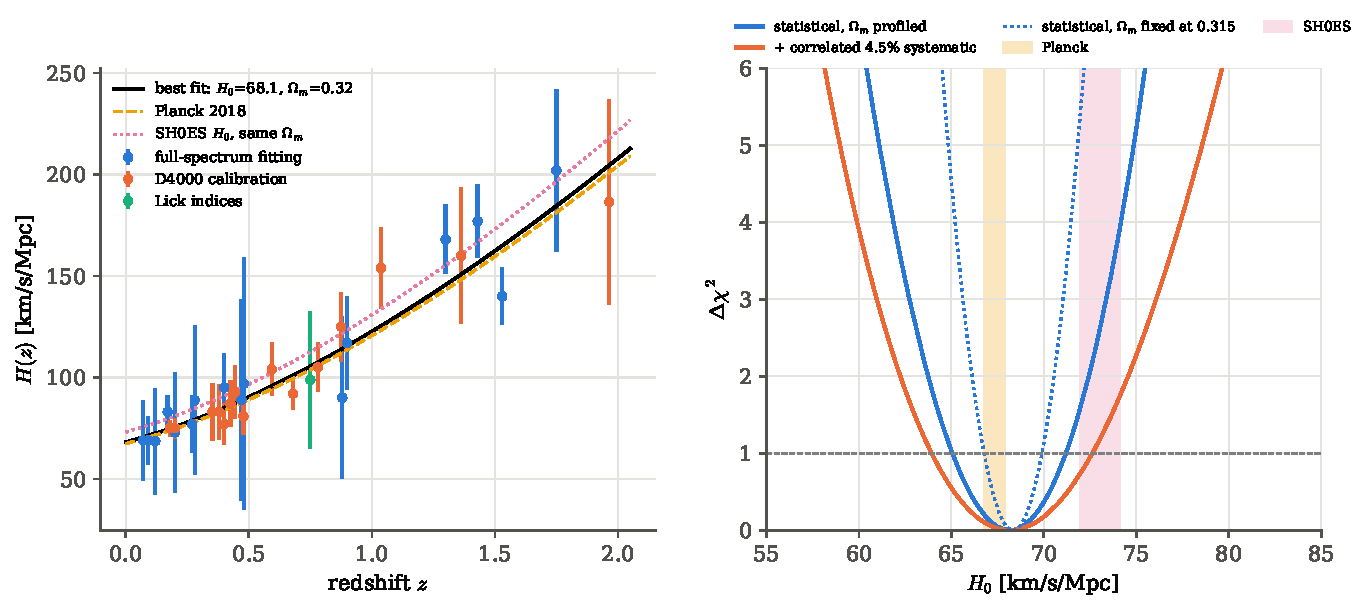
\includegraphics[width=12.5cm]{figures/ch11/chronometers.pdf}
\caption{Left: the $\FBCcN$ chronometer measurements, coloured by how the ages were read,
with the best fit of flat $\Lambda$CDM, the Planck 2018 expansion history, and the same
history with the SH0ES value of $H_0$. Right: $\Delta\chi^2$ as a function of $H_0$ with
$\Omega_{m0}$ fixed (dotted), profiled (blue), and profiled with the correlated
systematic (orange); the bands are Planck and SH0ES at $68\%$.}
\label{11c:fig:cc}
\end{figure}

\paragraph{Against the CMB and the ladder.} Treat the chronometer interval as Gaussian
with half-width $\FBCcSS$ (statistical) or $\FBCcSY$ (with the systematic). It differs from
Planck's $67.36\pm0.54$ by $\FBCcTenPlS$ standard deviations of the difference and from
SH0ES's $73.04\pm1.04$ by $\FBCcTenShS$ ($\FBCcTenShY$ with the systematic), the variance of a
difference of independent estimates being the sum of the variances. The chronometers
side with the CMB, but at less than two standard deviations from the ladder: on their
own they cannot decide the tension, as their compilers note \cite[Sec.~3.1.5.1]{Moresco2022}.
What they offer is independence: no distance ladder, and no early-Universe physics.

\paragraph{Three estimators, one structure.} The supernova estimator of
\cref{3b:sec:hubble}, Hubble's slope and the chronometer estimator are the same
calculation. In each, the parameter enters the model linearly (as a shift of
magnitudes, a multiplier of distances, a multiplier of $E(z)$), the maximum-likelihood
estimate is a weighted mean or ratio in closed form, and it sits on the
Cram\'er--Rao bound. And in each, something else enters as a common factor that the
fit cannot see: the absolute magnitude of the supernovae (\cref{3b:sec:hubble-degeneracy}),
Hubble's distance scale, the stellar-population slope $A$. The statistics delivers
$H_0$ only in units of a calibration that must come from outside the data.

\paragraph{The lesson.} Chronometers measure $H(z)$ with a clock instead of a ruler and
give $H_0=\FBCcHS\pm\FBCcSS$\,km/s/Mpc in flat $\Lambda$CDM ($\pm\FBCcSY$ with the shared
model error); their precision is limited not by the number of galaxies but by a shared
model error, which a covariance carries and a weighted mean alone would hide.
\section{One constant, many routes}
\label{11c:sec:h0-routes}

The Hubble constant has come up in this book as $465$, as $70$, as $73.04$, as $67.36$, as
$68.1$ and as $69.9$. Hubble's own slope, \cref{11c:sec:hubble1929}, was off from
today's by a factor of $6.6$, and nobody speaks of a tension about it. The ladder and the
CMB differ by $8\%$, and the disagreement is called a crisis. What separates the two
cases? Not the size of the gap. In Hubble's case the error bar was about $10\%$ and the distance scale was
unknown; in the modern case the error bars are $1.4\%$ and $0.8\%$.

So a list of numbers cannot settle anything. For each number we need two answers. First,
\emph{what was actually observed, and what had to be brought in from outside to turn it
into a value of $H_0$?} Second, \emph{given the errors, would two such numbers be expected to
differ by this much if they measured the same quantity?} The first is physics, and decides
which routes can disagree for a reason. The second is statistics, and decides how
surprised to be. We take them in that order.

\subsection{What each route observes, and what it must borrow}
\label{11c:sec:h0-borrow}

$H_0$ is a velocity per length, km/s per Mpc. A redshift gives the velocity (at low
redshift, $v=cz$, up to the peculiar velocities of \cref{11c:sec:pecvel}). The length is
never read off the sky. Every route observes something that is not $H_0$ and combines it
with one quantity borrowed from outside the data. Four examples show the pattern, one
for each way a length or a time enters.

\paragraph{A brightness, and the true brightness of the candle.} The supernovae of
\cref{3b:sec:hubble-degeneracy} observe the apparent magnitude $m$ at redshift $z$. At low
redshift the luminosity distance is $D_L=cz/H_0$, and the distance modulus relates it to
the absolute magnitude $M$ of the candle, with $D_L$ in Mpc. Call
$\alpha\equiv m-5\log_{10}(cz)$ the quantity the Hubble-flow supernovae determine:
\begin{align}
  \alpha
  &\eqby{1}M+5\log_{10}D_L+25-5\log_{10}(cz)
   \eqby{2}M+25-5\log_{10}H_0,\nonumber\\
  H_0
  &\eqby{3}10^{(M+25-\alpha)/5},\qquad
  \frac{\delta H_0}{H_0}\eqby{4}\frac{\ln10}{5}\,\delta M .
  \label{11c:eq:h0-candle}
\end{align}
\begin{explain}
  \item The distance modulus $m=M+5\log_{10}D_L+25$, subtracting $5\log_{10}(cz)$ from both sides.
  \item Put $D_L=cz/H_0$: the $5\log_{10}(cz)$ cancels, leaving $-5\log_{10}H_0$.
  \item Solve for $H_0$, with the observed $\alpha$ fixed.
  \item With $\alpha$ fixed, $\delta\ln H_0=\ln10\;\delta\log_{10}H_0=\ln10\,\delta M/5$, since
        $\log_{10}H_0=(M+25-\alpha)/5$.
\end{explain}
The data fix the combination $M-5\log_{10}H_0$ and nothing else, the degeneracy of
\cref{3b:sec:hubble-degeneracy}. The absolute magnitude $M$ is the borrowed quantity. It
comes from Cepheids anchored by geometry (\cref{T2b:sec:ladder}). A shift of $\delta M=0.18$\,mag
moves $H_0$ by about $8\%$, the size of the Hubble tension. Hubble's $465$ is the
same equation with a wrong $M$: the distances he assumed, from the brightest stars of
each nebula, were short by a factor $6.6$ (\cref{11c:sec:hubble-scale}), and $K=sH_0$ for a
distance scale off by a factor $s$.

\paragraph{An angle, and the length of a ruler.} A feature of known comoving length $r$
(the sound horizon $r_d$ for baryon acoustic oscillations, $r_s$ at recombination for the CMB
peaks) at comoving distance $D_M$ subtends the angle $\theta=r/D_M$. In a flat universe
$D_M=c\int_0^z\dd z'/H(z')=(c/H_0)\,I(z)$, where $I(z)=\int_0^z\dd z'/E(z')$ is a number
once the shape of $E(z)=H(z)/H_0$ is fixed. Then
\begin{align}
  \theta
  &\eqby{1}\frac{r}{D_M}
   \eqby{2}\frac{rH_0}{c\,I(z)},\qquad
  H_0\eqby{3}\frac{c\,I(z)\,\theta}{r},\qquad
  \frac{\delta H_0}{H_0}\eqby{4}-\frac{\delta r}{r}.
  \label{11c:eq:h0-ruler}
\end{align}
\begin{explain}
  \item The definition of the subtended angle of a ruler of length $r$ at distance $D_M$.
  \item Substitute $D_M=cI/H_0$.
  \item Solve for $H_0$.
  \item Hold the observed $\theta$ and the integral $I$ fixed: $\ln H_0=\ln(cI\theta)-\ln r$.
\end{explain}
The borrowed quantity is the ruler $r$, a length computed from the physics before
recombination (\cref{T2b:sec:bao}). The inverse ladder of \cref{T2b:sec:bao} is this equation with
$r_d=147.09$\,Mpc. For the CMB the integral $I$ also depends on $H_0$ through
$\Omega_{m0}=\omega_m/h^2$ (\cref{10a:sec:cmb-planck}), so $H_0$ is found by solving
$\theta_{\rm MC}=r_s/D_M$ rather than by rearranging it; the lever on the ruler remains.
The CMB borrows a second thing: to carry the result from $z\approx1100$ to today it
assumes the flat $\Lambda$CDM expansion history.

\paragraph{A redshift step, and a time step.} Chronometers observe the difference $\Delta z$
between two passively ageing galaxy populations and the difference $\Delta t$ of their ages,
and give $H(z)=-\Delta z/[(1+z)\Delta t]$ (\cref{3b:sec:hubble-cc}); $H_0=H(z)/E(z)$ then needs
the shape of $E$. The borrowed quantity is the age scale: stellar-population models turn a
spectrum into an age, and their error is a common fractional factor $\eta\approx4.5\%$
(\cref{11c:sec:cc-gls}). There is no distance in it at all.

\paragraph{A velocity profile, and the flow we are caught in.} A fit of velocity against
distance in our own neighbourhood needs, besides $H_0$, the peculiar flow. The joint fit of
\cref{11c:sec:virgo} recovers $H_0$ together with the infall speed, which is the borrowed
quantity here; the same sample fitted without the infall comes out low. The finite volume
adds a random error on top, the cosmic variance of \cref{11c:sec:cosmicvar}.

\paragraph{The shape they share.} Write any route as $H_0=O/X$, the observable $O$ divided by a
borrowed quantity $X$. Take logarithms: $\ln H_0=\ln O-\ln X$. If the errors of $O$ and
$X$ are independent and small, their variances add:
\begin{equation}
  \Bigl(\frac{\sigma_{H_0}}{H_0}\Bigr)^2=\Bigl(\frac{\sigma_O}{O}\Bigr)^2+\Bigl(\frac{\sigma_X}{X}\Bigr)^2 .
  \label{11c:eq:h0-budget}
\end{equation}
Observing more supernovae, more galaxies or more acoustic peaks shrinks the first term as
$1/N$. The second term is the error on one number that every measurement in the route
shares, and it does not shrink at all, as in the shared factor $\eta$ of
\cref{11c:sec:cc-gls}. The routes differ in which number they borrow, and each route's
borrowed number is a different physical quantity with its own independent error.
\Cref{11c:tab:h0-borrow} lists them; \cref{11c:tab:h0-values} gives the values obtained in the book
and in the literature.

\begin{table}[htbp]
\centering
\small
\renewcommand{\arraystretch}{1.25}
\begin{tabular}{@{}p{3.1cm}p{3.7cm}p{4.4cm}p{3.5cm}@{}}
\toprule
Route & Observed & Borrowed from outside & Derived in\\
\midrule
Toy Hubble diagram, Hubble 1929 &
  velocities and brightnesses of galaxies &
  the absolute brightness of the candle (the distance scale) &
  \cref{3b:sec:hubble,11c:sec:hubble1929}\\
Distance ladder &
  magnitudes of Cepheids and of Hubble-flow supernovae &
  $M$ from geometric anchors, one common value across rungs &
  \cref{3b:sec:hubble-degeneracy,T2b:sec:ladder}\\
CMB &
  angles and heights of the acoustic peaks &
  $r_s$ from early-Universe physics, and flat $\Lambda$CDM from $z\approx1100$ to now &
  \cref{10a:sec:cmb-planck}\\
BAO, inverse ladder &
  angle and redshift extent of the baryon feature in galaxy catalogues &
  $r_d$, from the CMB or from nucleosynthesis, and the shape of $E(z)$ &
  \cref{T2b:sec:bao,11a:sec:bao-desi}\\
Cosmic chronometers &
  redshift steps and age steps of old galaxies &
  stellar-population models for the ages ($\eta\approx4.5\%$) &
  \cref{3b:sec:hubble-cc,11c:sec:cc}\\
Local infall &
  velocities and distances in our neighbourhood &
  the infall pattern $v_{\rm inf}\,g(\bm x)$ &
  \cref{11c:sec:virgo}\\
Local cosmic variance &
  the density contrast in the volume used &
  an error floor, not a route &
  \cref{11c:sec:cosmicvar}\\
Combining a chain with a prior on $H_0$ &
  a posterior sample and a new Gaussian measurement &
  reweighting, valid only if the two overlap &
  \cref{9c:sec:importance}\\
\bottomrule
\end{tabular}
\caption{The routes to $H_0$ in the book: what each observes and what it must bring in from
outside to become a Hubble constant.}
\label{11c:tab:h0-borrow}
\end{table}

\begin{table}[htbp]
\centering
\small
\renewcommand{\arraystretch}{1.25}
\begin{tabular}{@{}p{4.0cm}p{3.8cm}p{4.5cm}@{}}
\toprule
Route & The book's own value & Published value\\
\midrule
Toy Hubble diagram, supernovae mock & mock truth $70$, recovered at the Cram\'er--Rao bound & --\\
Hubble 1929, $24$ nebulae & $465\pm56$ & $465\pm50$ (his table, solar-motion solution)\\
Local infall, mock sample & $69.9\pm0.3$ with the infall, $65.5$ without & --\\
Distance ladder & mock truth $73$, fit $73.90\pm1.10$ & SH0ES: $73.04\pm1.04$\\
CCHP TRGB ladder & -- & $69.8\pm1.7$\\
CMB & Fisher forecast $\sigma=0.53$ (TT,TE,EE+lowE) & Planck 2018: $67.36\pm0.54$ ($0.60$ without lensing)\\
BAO, inverse ladder & $69.2\pm0.9$ with the CMB $r_d$ & DESI: $69.29\pm0.87$ (CMB $r_d$), $68.53\pm0.80$ (BBN $r_d$)\\
Cosmic chronometers & $68.1\pm3.1$ ($\pm4.3$ with $\eta$) & --\\
Chain of \cref{9c:sec:importance} & $67.06\pm0.93$ & --\\
\bottomrule
\end{tabular}
\caption{The values of $H_0$ in km/s/Mpc. A mock value is a number the script was told to
find and then found, not a measurement. The BAO and CMB values share the sound horizon when
the CMB $r_d$ is used, and are not independent.}
\label{11c:tab:h0-values}
\end{table}

\subsection{Is the gap too big? The same gap in three sets of error bars}
\label{11c:sec:h0-gap}

Two routes give $H_A\pm\sigma_A$ and $H_B\pm\sigma_B$, and the errors are independent. Suppose both measure
the same constant. Then $D=H_A-H_B$ has mean zero. The variance of a difference of
independent variables is the sum of their variances, so $D$ has standard deviation
$\sigma_D=\sqrt{\sigma_A^2+\sigma_B^2}$, and the surprise is $|D|/\sigma_D$ standard deviations.
For the ladder and the CMB:
\begin{align}
  \frac{|D|}{\sigma_D}
  &\eqby{1}\frac{73.04-67.36}{\sqrt{1.04^2+0.54^2}}
   \eqby{2}\frac{5.68}{\sqrt{1.082+0.292}}
   \eqby{3}\frac{5.68}{1.172}
   =4.8 .
  \label{11c:eq:h0-sigma}
\end{align}
\begin{explain}
  \item SH0ES against Planck, with their quoted errors.
  \item The squares of the errors.
  \item Their sum has square root $1.172$.
\end{explain}
For a Gaussian, a difference this many standard deviations from zero in either direction has
probability of order $10^{-6}$. This is the value we use for the Hubble tension throughout.
Other places in the book get different numbers, with the same gap and different errors:

\begin{table}[htbp]
\centering
\small
\renewcommand{\arraystretch}{1.25}
\begin{tabular}{@{}p{3.4cm}p{3.0cm}p{1.8cm}p{1.7cm}p{3.0cm}@{}}
\toprule
Pair & Gap [km/s/Mpc] & $\sigma_D$ & $|D|/\sigma_D$ & Where\\
\midrule
SH0ES $73.04\pm1.04$ against Planck $67.36\pm0.54$ & $5.68$ & $1.17$ & $4.8$ & \cref{T2b:sec:tension}\\
SH0ES against the book's chain $67.06\pm0.93$ & $5.98$ & $1.40$ & $4.3$ & \cref{9c:sec:importance}\\
Riess 2011 $73.8\pm2.4$ against Planck 2013 $67.8\pm0.8$ & $6.0$ & $2.53$ & $2.4$ & \cref{11c:sec:marra}\\
\bottomrule
\end{tabular}
\caption{One gap of about $6$\,km/s/Mpc, three significances. The gap has barely moved in
a decade. The error has shrunk from $2.5$ to $1.2$.}
\label{11c:tab:h0-gap}
\end{table}

The $4.3$ differs from $4.8$ only because our chain, fitted to one simulated temperature
spectrum, is wider than Planck's final result ($0.93$ against $0.54$): a larger $\sigma_D$
under the same gap. The $2.4$ is the same arithmetic on the numbers of 2013: the ladder
then had an error of $2.4$ and Planck $0.8$. A gap of $6$ which was
$2.4$ standard deviations in 2013 has become $4.8$ as the error bars shrank, while the gap
stayed. That is the sense in which the tension is a statement about precision.

\paragraph{The other routes, against both camps.} The same arithmetic gives where each independent
route sits relative to the two:

\begin{table}[htbp]
\centering
\small
\renewcommand{\arraystretch}{1.25}
\begin{tabular}{@{}lrrr@{}}
\toprule
Route & $H_0$ & against SH0ES & against Planck\\
\midrule
CCHP TRGB & $69.8\pm1.7$ & $1.6\sigma$ & $1.4\sigma$\\
BAO with BBN $r_d$ (DESI) & $68.53\pm0.80$ & $3.4\sigma$ & $1.2\sigma$\\
Chronometers, ours (statistical) & $68.1\pm3.1$ & $1.5\sigma$ & $0.2\sigma$\\
Chronometers, ours (with $\eta$) & $68.1\pm4.3$ & $1.1\sigma$ & $0.2\sigma$\\
\bottomrule
\end{tabular}
\caption{Significance of each route's difference from the ladder and from the CMB, each with the
rule $|D|/\sqrt{\sigma_A^2+\sigma_B^2}$.}
\label{11c:tab:h0-pulls}
\end{table}

For instance, BAO with a big-bang-nucleosynthesis ruler against the ladder is
$(73.04-68.53)/\sqrt{1.04^2+0.80^2}=4.51/1.31=3.4$. The chronometers are consistent with
everyone, and so decide nothing. The independent BAO value, which uses neither the CMB peaks
nor the ladder, sits with the CMB.

\subsection{Two calibrations, not two expansion rates}
\label{11c:sec:h0-calibrations}

The expansion rate today is one number. What the tension compares is two chains of
inference, each ending in that number, each with its own borrowed quantity. The late
route, the ladder, borrows the absolute magnitude $M$ and a flow model, and assumes that supernovae are the same
kind of candle in Cepheid hosts and in the Hubble flow. The early route borrows the
sound horizon $r$ and the history of expansion from $z\approx1100$. If the two disagree,
by \eqref{11c:eq:h0-candle} and \eqref{11c:eq:h0-ruler} some borrowed quantity is off:
\begin{align}
  \delta M&\eqby{1}\frac{5}{\ln10}\ln\frac{73.04}{67.36}=2.171\times0.0810=0.18\ \text{mag},\nonumber\\
  r_d&\eqby{2}147.09\times\frac{69.29}{73.04}=139.5\ \text{Mpc}\quad(\text{a } 5.1\%\text{ shorter ruler}).
  \label{11c:eq:h0-closing}
\end{align}
\begin{explain}
  \item Invert \eqref{11c:eq:h0-candle}: $\delta H_0/H_0=\ln(73.04/67.36)=0.0810$ must come from a shift of
        $M$; this is $5\log_{10}(73.04/67.36)=0.18$ in magnitudes.
  \item By \eqref{11c:eq:h0-ruler}, $H_0\propto1/r_d$ with $\theta$ fixed, so a ruler of
        $147.09\times69.29/73.04$ would turn the inverse ladder's $69.29$ into $73.04$.
\end{explain}
Either a candle $0.18$ mag brighter than assumed, or a ruler $5\%$ shorter. These are
the two sizes of the problem. Neither can be tested on the ladder or on the CMB alone,
because each calibration is a single number that all its data share
(\cref{11c:eq:h0-budget}). That is why the way forward is a third route with a different borrowed
quantity: chronometers borrow neither, BAO borrows $r_d$ but from nucleosynthesis, and
the tip of the red-giant branch borrows a different candle. They sit between, closer to
the CMB, with errors still too large to say that the ladder is wrong.

\paragraph{What local cosmic variance can explain.} The ladder's volume is finite, and a
density contrast averaged over it changes the expansion seen from inside (\cref{11c:eq:infall}).
For the ladder's supernovae out to $z=0.15$ the spread of that effect is $1.25$ to
$1.5\%$ (\cref{11c:sec:tension-void}), about $1.1$\,km/s/Mpc, the size of the ladder's own
error. Suppose none of it were in the ladder's quoted $1.04$. Then the variances add:
$\sqrt{1.04^2+1.12^2}=1.53$, and
\[
  \frac{5.68}{\sqrt{1.53^2+0.54^2}}=\frac{5.68}{1.62}=3.5 .
\]
The tension would fall from $4.8$ to $3.5$ standard deviations. What cosmic variance cannot do
is produce the gap itself: $8.4\%$ is $5.5$ times the spread, which would need
the ladder's volume to be half empty, a fluctuation whose Gaussian probability is below
$10^{-7}$. Nor does it touch the CMB, the BAO ruler or the chronometers at $z$ up to $2$, which
use volumes far larger. Local effects bite hardest on the nearest samples: in the mock sample of
\cref{11c:sec:virgo}, within $30$\,Mpc, ignoring a $200$\,km/s infall moved $H_0$ from $69.9$ to $65.5$,
$6\%$, as large as the tension, but the ladder's supernovae lie beyond $z=0.023$, where the same $200$\,km/s is a few per
cent of each redshift, and are corrected with a flow model (\cref{11c:sec:research-shoes}).

\paragraph{The one-line lesson.} Every route to $H_0$ is an observable divided by a borrowed
calibration, the calibration does not average down, and the Hubble tension is the statement that two
calibrations, a luminosity and a ruler, disagree by $0.18$ mag, or $5\%$, at $4.8$ standard deviations.
\section{How the local Universe is measured in research}
\label{11c:sec:research}

The Cosmicflows-4 catalogue lists $55{,}877$ galaxies gathered into $38{,}065$
groups \cite{Tully2023CF4}. Each line holds a position on the sky, a redshift in the
frame of the cosmic microwave background, a distance with its error, and a peculiar
velocity. Every idea we have met since Hubble's diagram is somewhere behind those columns:
Hubble's fit of velocity against distance (\cref{11c:sec:hubble1929}), the velocity
field that structure induces (\cref{11c:sec:pecvel}), our own fall towards Virgo and
our motion through the microwave background (\cref{11c:sec:virgo}), the scatter of a
locally measured $H_0$ (\cref{11c:sec:cosmicvar}) and the bias of a distance read
off a noisy indicator (\cref{11c:sec:ihm}). The SH0ES distance ladder and the
chronometer compilation use the same ideas. Our scripts ran each of them once, on
Hubble's $24$ nebulae, on a few hundred simulated galaxies, or on a table of $32$
measurements. The question, in words:
\begin{quote}
\emph{At each step from a catalogue of distances, redshifts or ages to a published
$H_0$ or velocity field, what does a research analysis do that our scripts left out,
and which part of its error can more data shrink?}
\end{quote}

\Cref{11c:fig:research-chain} shows the three routes. The top row is the distance
ladder: geometry calibrates nearby stars, nearby stars calibrate brighter
indicators, and those reach the Hubble flow. The middle row is the map of galaxies
that predicts velocities, which the ladder uses to clean its redshifts. The bottom
row is the chronometer route, which uses no distances at all.

\begin{figure}[htbp]
\centering
\begin{tikzpicture}[scale=0.88,transform shape,
  bx/.style={draw=accent,thick,rounded corners=2pt,fill=ideabg,font=\footnotesize,
             minimum height=19mm,align=center,text width=27mm},
  sx/.style={draw=softgray,rounded corners=2pt,font=\footnotesize,align=center,
             text width=27mm,minimum height=13mm},
  flow/.style={->,thick,accent},
  side/.style={->,thick,softgray}]
\node[bx] (geo) at (0,0)    {geometry:\\ parallaxes,\\ masers,\\ eclipsing\\ binaries};
\node[bx] (cep) at (3.6,0) {Cepheids,\\ tip of the red\\ giant branch\\ ($\sim\!40$\,Mpc)};
\node[bx] (sec) at (7.2,0)  {SN\,Ia,\\ Tully--Fisher,\\ fundamental\\ plane, SBF,\\ SN\,II};
\node[bx] (hf)  at (10.8,0) {Hubble flow:\\ $H_0$ and\\ peculiar\\ velocities};
\draw[flow] (geo) -- (cep);
\draw[flow] (cep) -- (sec);
\draw[flow] (sec) -- (hf);
\node[sx] (rs)  at (3.6,-3.3) {redshift survey\\ (2M++): $\delta_g$};
\node[sx] (pv)  at (7.2,-3.3)  {predicted\\ velocities,\\ $\beta=f/b$,\\ bulk flow};
\draw[side] (rs) -- (pv);
\draw[side] (pv.east) -- (hf.south);
\node[sx] (pg)  at (3.6,-5.5) {passive galaxies:\\ age differences};
\node[sx] (hz)  at (7.2,-5.5)  {$H(z)$ from\\ $\dd z/\dd t$};
\node[sx] (h0)  at (10.8,-5.5) {$H_0E(z)$ with\\ a model\\ covariance};
\draw[side] (pg) -- (hz);
\draw[side] (hz) -- (h0);
\node[font=\scriptsize,text=softgray!70!black,anchor=east] at (1.75,-3.3) {velocity map};
\node[font=\scriptsize,text=softgray!70!black,anchor=east] at (1.75,-5.5) {no distances};
\end{tikzpicture}
\caption{Three routes to the local expansion. Top: the distance ladder, each rung
calibrating the next. Middle: a map of galaxy positions predicts peculiar velocities,
which are subtracted from the redshifts of the Hubble-flow objects. Bottom: cosmic
chronometers turn age differences of passive galaxies into $H(z)$ without any
distance.}
\label{11c:fig:research-chain}
\end{figure}

\subsection{Tens of thousands of distances: Cosmicflows-4}
\label{11c:sec:research-cf4}

Cosmicflows-4 combines eight ways of measuring a distance \cite[Sec.~1]{Tully2023CF4}.
Most galaxies have a distance from the Tully--Fisher relation \unpack{the luminosity of a
spiral galaxy predicted from its rotation speed} or the fundamental plane \unpack{the
same idea for an elliptical galaxy, using its velocity dispersion and surface
brightness}; each such distance is uncertain by $20$--$25\%$. Type~Ia supernovae give
about $7\%$ out to $z=0.1$, type~II supernovae about $15\%$, surface-brightness
fluctuations about $5\%$ out to $z\approx0.03$. Cepheids and the tip of the red giant
branch give about $5\%$ but only within about $20$\,Mpc; masers give six geometric
distances.

\paragraph{Putting eight methods on one scale.} Every subsample $s$ (one Tully--Fisher
survey, say) measures distance moduli with a zero point of its own. Call
$\mathrm{DM}^{(s)}_n$ the modulus of object $n$ (a group or a single galaxy) in
subsample $s$, $\Delta\mu_s$ an offset added to every modulus of that subsample, and
$\langle\mathrm{DM}\rangle_n$ the weighted mean of the adjusted moduli
$\mathrm{DM}^{(s)}_n+\Delta\mu_s$ over all subsamples that contain object $n$. With
independent Gaussian errors $\sigma_{n,s}$ on each difference, the log-likelihood of
the offsets is \cite[eqs.~(1)--(2)]{Tully2023CF4}
\begin{equation}
  -2\ln\Like(\Delta\bm\mu)
  =\sum_n\sum_{s\ni n}\frac{\bigl(\mathrm{DM}^{(s)}_n+\Delta\mu_s-\langle\mathrm{DM}\rangle_n\bigr)^2}{\sigma_{n,s}^2}
  +\text{const}.
  \label{11c:eq:cf4-like}
\end{equation}
For given offsets it asks how plausible the fluctuations are that must be added to the
adjusted moduli to make every object have one distance, the likelihood of
\cref{ch:03}. With a flat prior the posterior is this likelihood, and the
Cosmicflows team samples it with \pyname{emcee}, $128$ walkers of $10^4$ steps.

Two things follow from what we already know. First, each offset enters
\eqref{11c:eq:cf4-like} linearly, and so does $\langle\mathrm{DM}\rangle_n$, which is a
weighted mean of terms linear in the offsets. The exponent is therefore quadratic in
$\Delta\bm\mu$, the posterior is exactly Gaussian, and its mean and covariance follow
from one linear solve, as for every linear model since \cref{3b:sec:hubble}; the
chain is a check of that solve. Second, the overlaps cannot fix the overall zero
point. Add the same constant $c$ to every offset. With weights $w_{n,s}$,
\begin{align}
  \langle\mathrm{DM}\rangle_n(\Delta\bm\mu+c)
  &\eqby{1}\frac{\sum_sw_{n,s}\bigl(\mathrm{DM}^{(s)}_n+\Delta\mu_s+c\bigr)}{\sum_sw_{n,s}}
   \eqby{2}\langle\mathrm{DM}\rangle_n(\Delta\bm\mu)+c,
  \nonumber\\
  \mathrm{DM}^{(s)}_n+\Delta\mu_s+c-\langle\mathrm{DM}\rangle_n(\Delta\bm\mu+c)
  &\eqby{3}\mathrm{DM}^{(s)}_n+\Delta\mu_s-\langle\mathrm{DM}\rangle_n(\Delta\bm\mu).
  \label{11c:eq:cf4-shift}
\end{align}
\begin{explain}
  \item The definition of the weighted mean, with every offset shifted by $c$.
  \item Split the sum: the $c$ terms give $c\sum_sw_{n,s}/\sum_sw_{n,s}=c$.
  \item Subtract the first line: the two $c$'s cancel.
\end{explain}
Every residual, and so the likelihood, is unchanged: one direction in the space of
offsets is flat. Cosmicflows fixes it by setting the offset of its own Tully--Fisher
sample to zero. This is the third time the same thing has happened. Hubble's slope
could not see a common factor in his distances, \eqref{11c:eq:scale-invisible}, and a
supernova Hubble diagram cannot see the absolute magnitude
(\cref{3b:sec:hubble-degeneracy}). The absolute scale has to come from outside:
$542$ calibrator galaxies with distances from the tip of the red giant branch,
Cepheids or masers \cite[Sec.~10]{Tully2023CF4}.

\paragraph{Example: how small is the statistical error on $H_0$?} Each group $i$ gives a
Hubble parameter $H_i=f_iV_i/d_i$, its recession velocity $V_i$ in the microwave
background frame over its distance $d_i$, with $f_i$ a small correction to the
low-redshift Hubble law. Beyond $4000$\,km/s, where a peculiar velocity of
$300$\,km/s is less than $8\%$ of $V_i$, the mean of $\log_{10}H_i$ over about
$35{,}000$ groups is $1.8725$, that is $H_0=74.6$\,km/s/Mpc, and the scatter is
$0.091$ in $\log_{10}H$ \cite[Sec.~13]{Tully2023CF4}. How well does the mean pin down
$H_0$ if the groups are independent?
\begin{align}
  \sigma_{\log H_0}
  &\eqby{1}\frac{0.091}{\sqrt{35\,000}}=\FBLrCfSlog\times10^{-4},
  \nonumber\\
  \frac{\sigma_{H_0}}{H_0}
  &\eqby{2}\ln10\;\sigma_{\log H_0},
  \qquad
  \sigma_{H_0}=74.6\times2.303\times\FBLrCfSlog\times10^{-4}=\FBLrCfSH\ \text{km/s/Mpc}.
  \label{11c:eq:cf4-stat}
\end{align}
\begin{explain}
  \item The error of a mean of $N$ independent values is the scatter over $\sqrt N$.
  \item $\log_{10}H=\ln H/\ln10$, so $\dd\log_{10}H=\dd H/(H\ln10)$.
\end{explain}
A scatter of $0.091$ in $\log_{10}H$ is $\ln10\times0.091=\FBLrCfFrac\%$ per group, yet
the mean is fixed to about a thousandth. Cosmicflows quotes $\pm0.2$, more than twice
the naive figure; groups that fall together in one flow are not independent
(\cref{11c:sec:pv-corr}), so the naive figure is a floor. Either way the number is
small beside the $\pm0.8$ of the zero-point calibration and the possible systematic of
about $3$\,km/s/Mpc that the authors themselves state.

\paragraph{The calibration route decides the answer.} The value $74.6$ comes from
merging all eight methods onto one scale and tying that scale to $121$ calibrator
galaxies. Tying only the supernovae, through the $44$ supernova hosts with
Cepheid, red-giant or maser distances, gives $72.1$, close to the SH0ES value
\cite[Sec.~14]{Tully2023CF4}. The two routes use largely the same data, and they
differ by $2.5$\,km/s/Mpc, three times the statistical error. Hubble's lesson of
\cref{11c:sec:hubble-scale} survives ninety years and a factor of two thousand in the
number of galaxies: the fit delivers the expansion rate in units of a calibration, and
the error of the calibration does not average down.

\paragraph{Peculiar velocities from the catalogue.} The velocities in the catalogue use
the difference $cz-H_0d$ nearby and change over, by $3000$\,km/s, to the logarithmic
estimator of Watkins and Feldman \cite{WatkinsFeldman2015}, the one we derived in
\cref{11c:sec:log-estimator} to keep the noise Gaussian
\cite[eqs.~(9)--(11)]{Tully2023CF4}. For groups whose modulus is known to $0.10$\,mag
or better, the velocities have a roughly Gaussian distribution with standard deviation
$300$\,km/s. Linear theory with the Planck spectrum gave $\sigma_{v,1\mathrm D}=\FBPvSigOne$\,km/s
in \cref{11c:sec:pv-sigma}. The two numbers are not a like-for-like comparison: a
modulus error of $0.10$\,mag is a distance error of $(\ln10/5)\times0.10=\FBLrCfDist\%$,
which at $4000$\,km/s is $\FBLrCfVerr$\,km/s of velocity noise, so the measured width
contains both the motions and the errors. What the agreement in size does say is that
the galaxies move at the speeds linear theory predicts. Cosmicflows also finds larger
Hubble parameters in one part of the sky and smaller ones in the opposite part, the
dipole pattern of a bulk motion of the sample that we met in \cref{11c:sec:dipole}.

\subsection{Velocities predicted from a map of galaxies}
\label{11c:sec:research-recon}

A distance catalogue measures velocities and asks what mass moves them. The reverse
route needs no distances: take a redshift survey, which maps where the galaxies are,
and predict the velocities they must have. Carrick et al.\ did this with the 2M++
compilation, a redshift survey that maps the galaxy density out to $200\,h^{-1}$Mpc
\cite{Carrick2015}.

\paragraph{The prediction.} The linear velocity field of \cref{11c:sec:pv-linear} is
$\bm u(\bm x)=\frac{aHf}{4\pi}\int\dd^3x'\,\delta(\bm x')\,(\bm x'-\bm x)/|\bm x'-\bm x|^3$,
equation \eqref{11c:eq:u-integral}, where $\delta$ is the matter density contrast and $f$ the
growth rate. A survey sees galaxies, not matter. With the linear bias of
\cref{11a:sec:kaiser}, $\delta_g=b\,\delta$, the galaxy contrast is $b$ times the matter
contrast. Today $a=1$ and $H=H_0$, so
\begin{align}
  \bm u(\bm x)
  &\eqby{1}\frac{H_0f}{4\pi}\int\dd^3x'\,\frac{\delta_g(\bm x')}{b}\,
   \frac{\bm x'-\bm x}{|\bm x'-\bm x|^3}
   \eqby{2}\beta\,\frac{H_0}{4\pi}\int\dd^3x'\,\delta_g(\bm x')\,
   \frac{\bm x'-\bm x}{|\bm x'-\bm x|^3},
  \qquad \beta\equiv\frac fb .
  \label{11c:eq:beta-field}
\end{align}
\begin{explain}
  \item \eqref{11c:eq:u-integral} at $a=1$, $H=H_0$, with $\delta=\delta_g/b$.
  \item A constant comes out of the integral; name the ratio $f/b$.
\end{explain}
The map of galaxies predicts the whole velocity field up to one number, $\beta$. Call
$p_i$ the line-of-sight component of the integral at galaxy $i$, the velocity it would
have if $\beta$ were one.

\paragraph{The fit is Hubble's fit again.} A measured peculiar velocity $u_i$ with
error $\sigma_i$ (the distance error turned into velocity, plus a small-scale
dispersion that linear theory does not describe) is modelled as $u_i=\beta p_i+$noise.
Which $\beta$ makes the required noise most plausible?
\begin{align}
  \chi^2(\beta)
  &\eqby{1}\sum_i\frac{(u_i-\beta p_i)^2}{\sigma_i^2},
  \qquad
  \frac{\dd\chi^2}{\dd\beta}\eqby{2}-2\sum_i\frac{p_i\,(u_i-\beta p_i)}{\sigma_i^2}=0,
  \nonumber\\
  \hat\beta
  &\eqby{3}\frac{\sum_ip_iu_i/\sigma_i^2}{\sum_ip_i^2/\sigma_i^2},
  \qquad
  \Var\hat\beta\eqby{4}\Bigl(\sum_i\frac{p_i^2}{\sigma_i^2}\Bigr)^{-1}.
  \label{11c:eq:beta-hat}
\end{align}
\begin{explain}
  \item Gaussian noise: $-2\ln\Like$ is the $\chi^2$ up to a constant.
  \item Differentiate each square; the chain rule brings down $-p_i$.
  \item Solve the linear equation for $\beta$.
  \item The second derivative is $2\sum p_i^2/\sigma_i^2$; the variance of a
        maximum-likelihood estimate in a linear-Gaussian model is the inverse of half
        of it (\cref{ch:03}).
\end{explain}
This is Hubble's slope \eqref{11c:eq:k-origin} with $r_i\to p_i$, and the chronometer
estimator \eqref{11c:eq:cc-gls} with $E_i\to p_i$: a parameter that multiplies a known
template is estimated by a weighted ratio. Carrick et al.\ add a uniform velocity
$\bm V_{\rm ext}$, a \newterm{bulk flow} \unpack{a velocity shared by the whole mapped
volume, caused by mass outside it}, so that $u_i=\beta p_i+\bm V_{\rm ext}\cdot\hat{\bm r}_i$.
The model is still linear, now in four parameters, and the estimate is still one
matrix solve. Comparing with Tully--Fisher and supernova velocities they find
$\beta^*=0.431\pm0.021$ for their reference galaxies, which translates into
$f\sigma_8=0.401\pm0.024$, the same combination that redshift-space distortions measure
(\cref{11a:sec:fsigma8}), and a bulk flow of $159\pm23$\,km/s, preferred at $5.1$
standard deviations \cite{Carrick2015}.

\paragraph{Example: does the map explain our motion?} The 2M++ volume alone predicts a
Local Group velocity of $540$\,km/s towards galactic $(l,b)=(268^\circ,38^\circ)$; the
external bulk flow is $159$\,km/s towards $(304^\circ,6^\circ)$. The motion through
the microwave background found in \cref{11c:sec:dipole} is $\FBViLGspeed$\,km/s towards
$(\FBViLGl^\circ,\FBViLGb^\circ)$. Velocities add as vectors, so we need the angle between
the two directions. A direction $(l,b)$ is the unit vector
$(\cos b\cos l,\cos b\sin l,\sin b)$, and
\begin{align}
  \cos\theta
  &\eqby{1}\sin b_1\sin b_2+\cos b_1\cos b_2\cos(l_1-l_2)
   =\FBLrLgCos,\qquad\theta=\FBLrLgAng^\circ,
  \nonumber\\
  |\bm v_1+\bm v_2|^2
  &\eqby{2}v_1^2+v_2^2+2v_1v_2\cos\theta
   =540^2+159^2+2\times540\times159\times\FBLrLgCos,
  \nonumber\\
  |\bm v_1+\bm v_2|
  &=\FBLrLgSpeed\ \text{km/s}.
  \label{11c:eq:lg-sum}
\end{align}
\begin{explain}
  \item The dot product of the two unit vectors; the $\cos b_1\cos b_2$ terms combine
        through $\cos l_1\cos l_2+\sin l_1\sin l_2=\cos(l_1-l_2)$.
  \item $|\bm v_1+\bm v_2|^2=(\bm v_1+\bm v_2)\cdot(\bm v_1+\bm v_2)$, expanded.
\end{explain}
The sum points to $(\FBLrLgL^\circ,\FBLrLgB^\circ)$, $\FBLrLgAngCMB^\circ$ from the dipole
direction, and its size is within $7\%$ of the measured $620\pm15$\,km/s. Most of our
motion is pulled by structure within $200\,h^{-1}$Mpc; the rest, a bulk flow of
$159$\,km/s, comes from farther away.

\subsection{Flow corrections in the supernova ladder}
\label{11c:sec:research-shoes}

The third rung of the SH0ES ladder is $277$ supernovae with $0.0233<z<0.15$
\cite{Riess2022SH0ES}. Each one's redshift contains a peculiar velocity, which the
Hubble law reads as a wrong distance.

\paragraph{How far does an unknown velocity move one supernova?} The distance modulus
of a source at luminosity distance $d$ is $\mu=5\log_{10}(d/10\,\mathrm{pc})$; at low
redshift the predicted distance is $d=cz/H_0$. By \eqref{11c:eq:vpec-z}, the observed
$cz$ is $H_0r+u_r$, the Hubble flow plus the line-of-sight peculiar velocity $u_r$.
Treating $u_r$ as a small change of $cz$,
\begin{align}
  \mu
  &\eqby{1}5\log_{10}\frac{cz}{H_0\cdot1\,\mathrm{Mpc}}+25,
  \qquad
  \delta\mu\eqby{2}\frac{5}{\ln10}\,\frac{\delta(cz)}{cz}
  \eqby{3}\frac{5}{\ln10}\,\frac{u_r}{cz},
  \nonumber\\
  \sigma_\mu
  &\eqby{4}\frac{5}{\ln10}\,\frac{\sigma_v}{cz}\approx2.17\,\frac{\sigma_v}{cz}.
  \label{11c:eq:sigma-mu-v}
\end{align}
\begin{explain}
  \item $d$ in Mpc: $5\log_{10}(d\times10^6\,\mathrm{pc}/10\,\mathrm{pc})=5\log_{10}d+25$.
  \item $\dd\log_{10}x=\dd x/(x\ln10)$, the same identity as in \eqref{11c:eq:cf4-stat}.
  \item The change of $cz$ is the peculiar velocity.
  \item A velocity scatter $\sigma_v$ gives a scatter in $\mu$ larger by the same factor.
\end{explain}
For $\sigma_v=250$\,km/s this is $\FBLrMuTwoFiftyA$\,mag at $z=0.01$, $\FBLrMuTwoFiftyB$\,mag at
$z=0.0233$ and $\FBLrMuTwoFiftyC$\,mag at $z=0.15$ (\cref{11c:fig:local-research}, left). After
standardisation, nearby supernovae scatter about the Hubble line by
$0.16$--$0.17$\,mag all told, velocities included \cite{Peterson2022}. At $z=0.01$ a
velocity of the typical size is as large as that whole scatter; at $z=0.0233$ it is
half of it in magnitudes, a quarter in variance. The lower cut keeps the supernovae
whose distances the velocities barely disturb; the upper cut, $z=0.15$, keeps the
Hubble law nearly independent of the matter density. Pantheon+ puts the remaining
velocity scatter into each supernova's error as a term $\sigma_{v_{\rm pec}}$, computed
from $240$\,km/s and converted to magnitudes as in \eqref{11c:eq:sigma-mu-v} \cite[eq.~(3), Sec.~3.1.3]{Brout2022PantheonPlus}.

\begin{figure}[htbp]
\centering
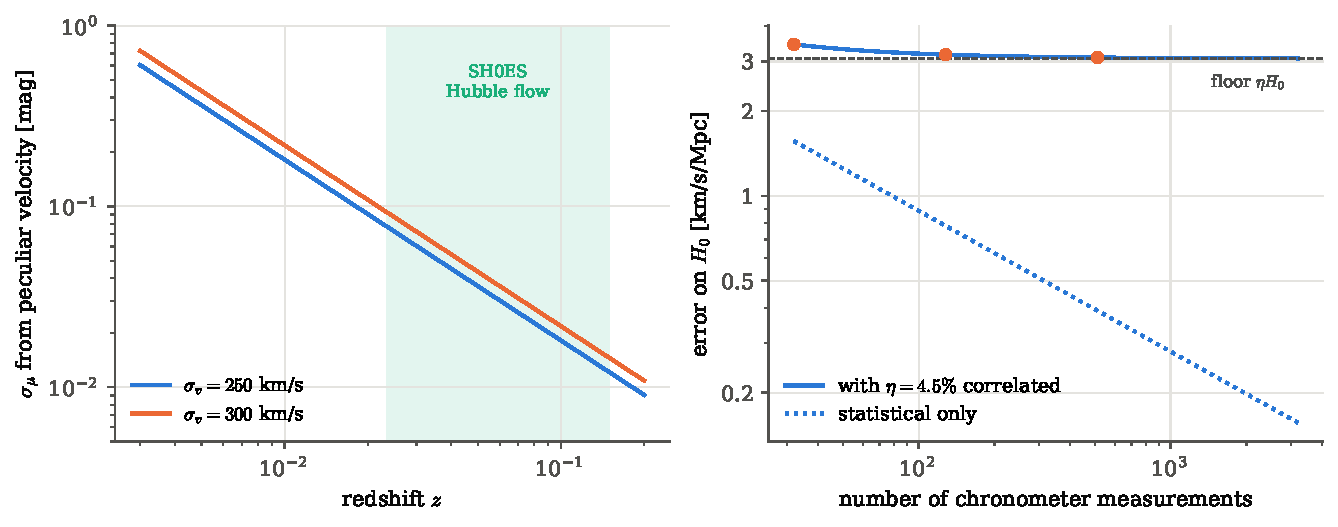
\includegraphics[width=12.5cm]{figures/ch11/local_research.pdf}
\caption{Left: the scatter in a supernova's distance modulus caused by an unmodelled
peculiar velocity, for two velocity dispersions; the shaded band is the redshift range
of the SH0ES Hubble-flow sample. Right: the error on $H_0$ from cosmic chronometers as
the compilation grows, with only statistical errors (dotted) and with a $4.5\%$ error
shared by all points (solid), which levels off at $\eta H_0$; the dots are the full
generalised least-squares fit to $1$, $4$ and $16$ stacked copies of the data.}
\label{11c:fig:local-research}
\end{figure}

\paragraph{Correcting the redshifts.} Pantheon+ corrects the redshifts in two steps
\cite{Peterson2022}. A supernova in a group gets the group's mean redshift, which
removes the orbital motion inside the group. Then the velocity predicted from the
2M++ map, \eqref{11c:eq:beta-field}, is subtracted. Together the corrections reduce
the scatter of $584$ nearby supernovae about the Hubble line from $0.167$ to
$0.157$\,mag and raise $H_0$ by about $0.4$\,km/s/Mpc; the choice among velocity maps
leaves a systematic uncertainty of only $0.06$--$0.11$\,km/s/Mpc in $H_0$. In the SH0ES fit, dropping the corrections
lowers $H_0$ by $0.5$, and dropping every supernova below $z=0.06$ raises it by $0.3$
\cite[Secs.~6.8, 6.12]{Riess2022SH0ES}. As the SH0ES team notes, both changes go the
wrong way for the idea that we sit in an underdense region that raises the local $H_0$
(\cref{11c:sec:tension-void}): in such a hole, removing the nearest supernovae would
lower $H_0$, and so would correcting for the outflow. What the corrections cannot
remove is the part of the scatter in $H_0$ that comes from structure beyond the map, the
cosmic variance of \cref{11c:sec:cosmicvar}; for this redshift range it is estimated
at $0.5$--$1\%$ \cite[Sec.~IV.F]{Abdalla2022}.

\paragraph{Example: why not use the Cepheid hosts' own redshifts?} The $37$ galaxies
with Cepheids have a mean $cz$ of about $2000$\,km/s \cite[Sec.~6.12]{Riess2022SH0ES}. If
their redshifts were used directly, a velocity of $250$\,km/s would be
$250/2000=\FBLrHostFrac\%$ of each one's Hubble velocity. For $37$ independent
velocities the mean would be uncertain by $\FBLrHostFrac\%/\sqrt{37}=\FBLrHostMean\%$.
The velocities are not independent: galaxies within a few tens of megaparsecs share
most of their motion (\cref{11c:sec:pv-corr}). The SH0ES team, using the spatial
covariance of the flows, finds that this two-rung route is limited to $3$--$4\%$. If
the velocities alone set that number, the $37$ hosts are worth about
$(12.5/3.5)^2\approx13$ independent ones. A third rung reaching $z>0.023$ is what
makes a $1\%$ measurement possible.

\subsection{Chronometers: what the error budget is made of}
\label{11c:sec:research-cc}

A cosmic chronometer (\cref{11c:sec:cc}) reads $H(z)=-(1+z)^{-1}\dd z/\dd t$ from the
age difference $\dd t$ of passively evolving galaxies at nearby redshifts. The ages
come from spectral features, such as the $4000$\,\AA\ break, through slopes computed
with \newterm{stellar population synthesis} models \unpack{models that predict the
spectrum of a population of stars from its age, metallicity and history}. Moresco
et al.\ split the covariance of the $H(z)$ points into a statistical part and four
systematic ones \cite[Sec.~3.1.4, eqs.~(19)--(21)]{Moresco2022}:
\begin{equation}
  C=C^{\rm stat}+C^{\rm met}+C^{\rm young}+C^{\rm model},
  \qquad
  C^{\rm model}=C^{\rm SFH}+C^{\rm IMF}+C^{\rm lib}+C^{\rm SPS}.
  \label{11c:eq:cc-budget}
\end{equation}
Each term answers a question about the galaxies. \emph{Is the metallicity right?} A
$10\%$ error in the stellar metallicity gives about a $10\%$ error in $H$; it belongs
to each spectrum separately, so it is diagonal. \emph{Did the stars form in one burst?}
Assuming so when the star formation lasted up to $0.3$\,Gyr costs $2$--$3\%$, again
diagonal. \emph{Is there a young component hiding in an old galaxy?} If $10\%$ ($1\%$)
of the light came from young stars, $H$ would be off by $5\%$ ($0.5\%$); in the samples
used so far the contamination is below detection and the effect below $0.5\%$.
\emph{Is the population model right?} Changing the synthesis model shifts $H$ by about
$4.5\%$, the initial mass function by less than $0.4\%$, the stellar library by
somewhat more \cite{Moresco2020}. These shifts move every point the same way, so they
are treated as fully correlated across redshift. The three diagonal terms are already
inside the published errors of \cref{11c:tab:cc-data}. Errors that include a
conservative systematic allowance do not show up as scatter, which is the reading we gave of
the small $\chi^2$ in \cref{11c:sec:cc-fit}. The correlated model term must be added by
the user; we added it as a single $\eta=4.5\%$.

\paragraph{More galaxies do not help.} \Cref{11c:sec:cc-gls} showed that a fully
correlated fractional error $\eta$ adds in quadrature,
$\sigma^2_{H_0}=\sigma^2_{\rm stat}+(\eta H_0)^2$, equation \eqref{11c:eq:cc-sys}. Suppose we had
$k$ compilations of the same quality instead of one. The statistical variance falls as
$1/k$; the shared model error is the same in every copy:
\begin{align}
  \sigma^2_{H_0}(k)
  &\eqby{1}\frac{\sigma^2_{\rm stat}}{k}+(\eta H_0)^2
   \;\xrightarrow{\;k\to\infty\;}\;(\eta H_0)^2 .
  \label{11c:eq:cc-floor}
\end{align}
\begin{explain}
  \item \eqref{11c:eq:cc-sys} with $\bm E^{\mathsf T}D^{-1}\bm E$ multiplied by $k$, since
        $k$ independent copies add their Fisher information.
\end{explain}
With $\sigma_{\rm stat}=\FBLrCcSa$ and $\eta H_0=\FBLrCcFloor$\,km/s/Mpc, the error is
$\FBLrCcKone$ for the present data, $\FBLrCcKfour$ with four times as many and
$\FBLrCcKsixteen$ with sixteen times as many; the generalised least-squares fit on stacked
copies gives the same numbers (\cref{11c:fig:local-research}, right). The floor is
$\FBLrCcFloorPct\%$ of $H_0$. Moresco et al.\ reach the same conclusion by simulation: with
the current data they find $H_0=66.5\pm5.4$ in flat $\Lambda$CDM, and their optimistic
forecast reaches $69.0\pm2.1$ only if the synthesis-model term is resolved, leaving the
initial-mass-function term \cite[Sec.~3.1.6, Table~2]{Moresco2022}. In
\eqref{11c:eq:cc-floor} a $0.4\%$ floor is $\FBLrCcIMF$\,km/s/Mpc, below the statistical
error, so the data would again be limited by their number. Their current interval is
wider than ours ($\pm\FBCcSY$): their covariance contains the stellar-library term and a
redshift-dependent synthesis-model term on top of our single constant. The centres,
$66.5$ and $\FBCcHY$, differ by a third of either error.

\paragraph{A bias the differential method avoids.} At high redshift, a selection for
old passive galaxies may pick objects that are the ancestors of a different population
from the one selected nearby, and so flatten the age--redshift relation. Comparing only
galaxies at nearly the same redshift limits this \newterm{progenitor bias}; Moresco
et al.\ estimate it at about $1\%$ in $H$, small beside the model term.

\subsection{What our shortcuts cost}
\label{11c:sec:research-nerfs}

\Cref{11c:tab:nerfs} lists, for each calculation, what a research analysis does instead
and what our reduction costs. The reductions are of two kinds. Some only cost precision and
would shrink with computing time or data. Others leave out a physical ingredient, and no
amount of computing inside our model brings it back.

\begin{table}[htbp]
\centering
\small
\renewcommand{\arraystretch}{1.15}
\begin{tabular}{@{}p{0.14\linewidth}p{0.27\linewidth}p{0.26\linewidth}p{0.27\linewidth}@{}}
\toprule
section & research & ours & what it costs\\\midrule
Hubble 1929 & $5.6\times10^4$ galaxies, eight methods, zero points by MCMC, $542$ calibrators &
Hubble's $24$ nebulae, one velocity scatter, solar motion fitted &
nothing for the lesson; $H_0$ itself was off by a factor $\FBHubFacb$ in 1929\\
velocities & $N$-body and constrained simulations, nonlinear motions, galaxy bias &
linear theory from CAMB; $\FBPvNbox$ Gaussian boxes of $\FBPvBoxL\,h^{-1}$Mpc &
no motions inside groups and clusters; matter only\\
local flow & velocity field from 2M++ with $\beta$ and a bulk flow; Cosmicflows velocities &
one spherical attractor, power-law profile, $\FBViNgal$ simulated galaxies &
no external bulk flow (the $159$\,km/s of \cite{Carrick2015}); one attractor only\\
local $H_0$ & $N$-body box of $6\,h^{-1}$Gpc, observers in haloes and voids, the real supernova sky &
linear $P(k)$, three windows, Gaussian boxes of $\FBLhBoxL\,h^{-1}$Mpc &
no observer selection, no nonlinear density; linear rows agree within $0.1$ percentage point\\
Malmquist & joint likelihood of distances and a 3-D density map over the sky &
one line of sight through one cluster, lognormal errors &
no selection function, no sky coverage; the mechanism only\\
chronometers & full covariance \eqref{11c:eq:cc-budget}, redshift-dependent terms, sampled posteriors &
diagonal errors plus one constant $4.5\%$, grid profile over $\Omega_{m0}$ &
interval $\pm\FBCcSY$ instead of $\pm5.4$\,km/s/Mpc\\
\bottomrule
\end{tabular}
\caption{Each section's analysis at research scale and in the scripts, with the cost of
the reduction.}
\label{11c:tab:nerfs}
\end{table}

The row that matters most is the local flow. Our Virgo model has one attractor; the real
local Universe has the Great Attractor, Perseus--Pisces, the Shapley concentration and
a bulk flow from beyond them all. Everything statistical we derived (the linear
velocity field, the joint linear fit, the dilution by distance errors, the Malmquist
correction) carries over unchanged to a three-dimensional map; what does not carry over
is the claim that one parameter, $v_{\rm inf}$, describes the flow. Research replaces it
with \eqref{11c:eq:beta-field} evaluated on a real galaxy map, plus a bulk flow.

\begin{inpractice}[Checks, and instruments]
Four calculations on the local Universe checked an analytic result by simulation: the
velocity dispersion from $P(k)$ against Gaussian boxes ($\FBPvSigOneBox\pm\FBPvSigOneBoxScatter$
against $\FBPvSigOneTrunc$\,km/s), the window variance of a local $H_0$ against observers in
boxes ($\FBLhBoxHund\%$ against $\FBLhContHund\%$ at $100\,h^{-1}$Mpc), the Malmquist factor
against a simulated catalogue ($\FBMbUniSim$ against $\FBMbUniFac$), and the chronometer
errors against $\FBCcNmock$ mock compilations ($\FBCcMockYSd$ against $\FBCcMockYSdTh$). Each
time the simulation verified a formula we already had. Research uses the same tools
where no formula exists: Wojtak et al.\ needed an $N$-body simulation because
observers sitting in haloes see a nonlinear density; Moresco et al.\ sized the
synthesis-model error by simulating spectra with one model and analysing them with
the others; Pantheon+ measures the effect of its velocity model by refitting with an
alternative map, because no formula relates two maps.
\end{inpractice}

\paragraph{The lesson.} Every local measurement of the expansion is a weighted ratio of a
measured quantity to a template, whose statistical error falls as $1/\sqrt N$, multiplied
by a calibration that does not fall at all; the work of research is in the calibration
and in the correlated errors, which is where Hubble's $500$\,km/s/Mpc went wrong
and where the present tension will be decided.

\begin{recap}
\begin{itemize}[itemsep=1pt,leftmargin=1.2em]
  \item Hubble's $24$ nebulae, refitted with a solar motion, give his $K=\FBHubKb\pm\FBHubsKb$.
        The slope of a fit through the origin is $\sum v_ir_i/\sum r_i^2$; distance errors
        add $K^2\Delta^2r_i^2$ to the variance; a common factor in all distances is
        invisible to the fit, which is why $465$ became $70$ (\cref{11c:sec:hubble1929}).
  \item A redshift gives $u_r=c(z_{\rm obs}-z_c)/(1+z_c)$. Linear theory gives
        $\bm u=\frac{aHf}{4\pi}\int\delta\,(\bm x'-\bm x)/|\bm x'-\bm x|^3$, a velocity
        dispersion $\sigma_{v,1\mathrm D}=\FBPvSigOne$\,km/s from $P(k)/k^2$, and velocities
        correlated over $\sim\!100\,h^{-1}$Mpc (\cref{11c:sec:pecvel}).
  \item Infall towards a spherical overdensity is $-\frac13aHf\bar\delta(<R)R$; a joint
        linear fit recovers $H_0$ and the infall speed, and ignoring the infall biases $H_0$.
        The Local Group moves at $\FBViLGspeed$\,km/s through the microwave background
        (\cref{11c:sec:virgo}).
  \item A local least-squares $H_0$ sees the density through the window
        $15j_2(kR)/(kR)^2$, with $\delta H/H=-f\delta_W/3$; its scatter is about $1\%$ at
        $150\,h^{-1}$Mpc, reproducing Wojtak et al.\ and Marra et al., and far too small to
        explain the $\FBLhGap\%$ tension (\cref{11c:sec:cosmicvar}).
  \item A distance measured with lognormal error $\Delta$ in a density $n(r)$ has
        $E(r\given d)\approx d[1+(7/2+\gamma)\Delta^2]$: inhomogeneous Malmquist bias,
        which makes spurious outflows around clusters; the logarithmic velocity estimator
        keeps the noise Gaussian (\cref{11c:sec:ihm}).
  \item Chronometers give $H(z)=-(1+z)^{-1}\dd z/\dd t$; the generalised least-squares
        estimate is $\bm E^{\mathsf T}C^{-1}\bm H/\bm E^{\mathsf T}C^{-1}\bm E$, and a shared
        $4.5\%$ model error sets a floor $\eta H_0=\FBLrCcFloor$\,km/s/Mpc; flat $\Lambda$CDM gives
        $H_0=\FBCcHS$ with $[\FBCcLoY,\FBCcHiY]$ (\cref{11c:sec:cc}).
  \item Research adds tens of thousands of distances on one zero point, velocity
        maps with $\beta=f/b$, flow-corrected redshifts beyond $z=0.023$ where
        $\sigma_\mu=2.17\,\sigma_v/cz$ is small, and full systematic covariances
        (\cref{11c:sec:research}).
\end{itemize}
\end{recap}

\subsection*{Reading the literature}
\label{11c:sec:reading-list}

\begin{itemize}[itemsep=2pt,leftmargin=1.2em]
  \item \textbf{Statistics of the fits.} Cowan, \emph{Statistical Data Analysis},
        Chapters~6 and~7 on maximum likelihood and least squares
        \srcref{Cowan}{Chs.~6--7}; Hobson et al., \emph{Bayesian Methods in Cosmology},
        on survey design and forecasts \srcref{HobsonBMC}{\S5.3}.
  \item \textbf{Galaxies as points, and two-point estimators.} Peebles on the
        large-scale structure of the Universe \cite{Peebles1980}; Peebles and Hauser,
        Davis and Peebles, Hamilton, Landy and Szalay and Kerscher et al.\ on
        correlation-function estimators
        \cite{PeeblesHauser1974,DavisPeebles1983,Hamilton1993,LandySzalay1993,Kerscher2000};
        Feldman, Kaiser and Peacock on the power spectrum \cite{FKP1994}; Xavier et al.\ on
        lognormal fields \cite{Xavier2016}.
  \item \textbf{The acoustic peak and redshift-space distortions.} Eisenstein and Hu on
        the transfer function \cite{EisensteinHu1998}; Seo and Eisenstein on forecasts
        \cite{SeoEisenstein2003}; Eisenstein et al.\ on the first detection
        \cite{Eisenstein2005}; Percival and White, Anderson et al.\ and Alam et al.\ on
        BOSS \cite{PercivalWhite2009,Anderson2012,Alam2017}; DESI 2024 \cite{DESI2024VI};
        Kaiser on redshift-space clustering \cite{Kaiser1987}.
  \item \textbf{Beyond two points.} Bernardeau et al.\ on perturbation theory
        \cite{Bernardeau2002}; Cooray and Sheth on the halo model \cite{CooraySheth2002};
        Navarro, Frenk and White on halo profiles \cite{NFW1997}; Takahashi et al.\ on
        simulated skies \cite{Takahashi2017sims}.
  \item \textbf{The local Universe.} Hubble, and Hubble and Humason, on the expansion
        \cite{Hubble1929,HubbleHumason1931}; Baade and Sandage on the recalibration
        \cite{Baade1956,Sandage1958}; Hogg on distance measures \cite{Hogg1999}; Peebles
        on the linear velocity field \cite{Peebles1993}; G\'orski on velocity
        correlations \cite{Gorski1988}; Schechter on Virgocentric infall
        \cite{Schechter1980}; Lynden-Bell et al.\ on the Great Attractor
        \cite{LyndenBell1988}; Strauss and Willick's review of peculiar velocities and
        Malmquist bias \cite{StraussWillick1995}; Watkins and Feldman on the logarithmic
        estimator \cite{WatkinsFeldman2015}; Carrick et al.\ on velocities from 2M++
        \cite{Carrick2015}; Tully et al., Cosmicflows-4 \cite{Tully2023CF4}; Planck 2018
        for the dipole \cite{Planck2018I}.
  \item \textbf{$H_0$ and the tension.} Riess et al.\ (SH0ES) and Brout et al.\
        (Pantheon+) \cite{Riess2022SH0ES,Brout2022PantheonPlus}; Peterson et al.\ on flow
        corrections \cite{Peterson2022}; Marra et al.\ and Wojtak et al.\ on the cosmic
        variance of a local $H_0$ \cite{Marra2013,Wojtak2014}; Abdalla et al.\ for a review
        \cite{Abdalla2022}; Planck 2018 for the early-Universe value \cite{Planck2018VI}.
  \item \textbf{Cosmic chronometers.} Jimenez and Loeb on the idea \cite{JimenezLoeb2002};
        Moresco et al.\ on the $4000$\,\AA\ break, on systematics, and the review
        \cite{Moresco2016,Moresco2020,Moresco2022}.
\end{itemize}

\section*{Chapter summary}
\addcontentsline{toc}{section}{Chapter summary}
\label{11c:sec:summary}

A galaxy survey is a list of points, and no theory predicts any one of them. What a
model predicts is how the points cluster, so every number a survey yields comes from
asking one question about a list: if the points are a random sample of a smooth field,
what is the sampling distribution of a summary of their positions, and how does the
survey distort it? Poisson sampling adds the shot noise $1/\bar n$; a random catalogue
cancels the survey's edges in the Landy--Szalay estimator; a weight $1/(1+\bar nP)$
minimises the variance of the power spectrum; a dilation of a template measures the
acoustic ruler; the motions of galaxies squash the pattern by $(b+f\mu^2)^2$ and so
measure the growth rate. The two-point function does not see everything: fields with
the same $P(k)$ can look entirely different, and haloes, their abundance, their
profiles, and the voids between them carry the rest. In the local Universe the
velocities are measured directly, and the same estimators return in their simplest
form: Hubble's slope, the infall speed, $\beta$ and the chronometer $H_0$ are all
weighted ratios, each multiplied by a calibration the data cannot see. In the pipeline
\[
  \text{physical model}\to\boxed{\text{field or data}\to\text{summary }S\to P(S\given\theta)}\to\text{infer physics},
\]
galaxy clustering works the middle arrows for points rather than maps: how a sample of a
field becomes a summary, and what sampling, masks and motions do to its distribution.
\Cref{ch:12} takes the structures the two-point function misses into topological
summaries, \cref{ch:13} turns to the Planck data that set the early-Universe side of the $H_0$
comparison, and
\cref{ch:14} collects the ways in which an estimator and its calibration part company.

\begin{center}
\small
\renewcommand{\arraystretch}{1.15}
\begin{tabularx}{\linewidth}{@{}>{\raggedright\arraybackslash}p{3.3cm}
                               >{\raggedright\arraybackslash}X
                               >{\raggedright\arraybackslash}p{2.0cm}@{}}
\toprule
\multicolumn{3}{@{}l}{\textbf{Clustering of galaxies}}\\
concept & operational meaning & used later in\\\midrule
Cox process, shot noise & Poisson given $\bar n(1+\delta_g)$; counts-in-cells variance $\langle N\rangle+\langle N\rangle^2\sigma_R^2$; power $P(k)+1/\bar n$ & \cref{ch:12,ch:14}\\
lognormal field & $1+\delta=e^{G-\sigma_G^2/2}$: a positive density with a chosen spectrum, for mocks & \cref{ch:12}\\
Landy--Szalay & $(DD-2DR+RR)/RR$ against a random catalogue; edge terms cancel to first order & \cref{ch:14}\\
integral constraint & $\hat\xi$ is low by the mean of $\xi$ over the survey & \cref{ch:14}\\
FKP estimator & weighted data-minus-randoms field, $w=1/(1+\bar nP)$; information counted by $V_{\rm eff}$ & \cref{ch:14}\\
BAO dilation $\alpha$ & template fitted at $\alpha r$; $\alpha$ measures $D_V/r_d$; significance $\sqrt{\Delta\chi^2}$ peak against no peak & \cref{ch:13,ch:14}\\
Kaiser formula & $P_s(k,\mu)=(b+f\mu^2)^2P(k)$; multipoles $P_0,P_2,P_4$ & \cref{ch:14}\\
$f\sigma_8$ & the growth rate times the amplitude, measured by the quadrupole-to-monopole ratio & \cref{ch:13,ch:14}\\
fingers of God & small-scale velocities stretch clusters along the line of sight; a damping of $P_s$ & \cref{ch:14}\\
mocks & a thousand simulated surveys for the covariance; error bars only as good as the mocks & \cref{ch:14}\\
\bottomrule
\end{tabularx}
\end{center}

\begin{center}
\small
\renewcommand{\arraystretch}{1.15}
\begin{tabularx}{\linewidth}{@{}>{\raggedright\arraybackslash}p{3.3cm}
                               >{\raggedright\arraybackslash}X
                               >{\raggedright\arraybackslash}p{2.0cm}@{}}
\toprule
\multicolumn{3}{@{}l}{\textbf{Beyond two points: haloes and voids}}\\
concept & operational meaning & used later in\\\midrule
same $P(k)$, different field & two fields with identical spectra and different phases; the difference is in higher-order statistics & \cref{ch:12}\\
halo mass function & number of haloes per unit mass and volume, from the fraction of the smoothed field that has collapsed & \cref{ch:14}\\
halo bias & how much more strongly haloes of a given mass cluster than matter & \cref{ch:14}\\
halo profile & the density around a halo centre and its Fourier transform $u(k\given m)$ & \cref{ch:14}\\
halo model & $P(k)$ as a one-halo (pairs in one halo) plus a two-halo (pairs in two haloes) term & \cref{ch:14}\\
halo occupation & the mean number of galaxies in a halo of mass $m$, central and satellites & \cref{ch:14}\\
voids & large underdense regions; their abundance, profiles and shapes as summaries & \cref{ch:12,ch:14}\\
\bottomrule
\end{tabularx}
\end{center}

\begin{center}
\small
\renewcommand{\arraystretch}{1.15}
\begin{tabularx}{\linewidth}{@{}>{\raggedright\arraybackslash}p{3.3cm}
                               >{\raggedright\arraybackslash}X
                               >{\raggedright\arraybackslash}p{2.0cm}@{}}
\toprule
\multicolumn{3}{@{}l}{\textbf{The local Universe}}\\
concept & operational meaning & used later in\\\midrule
fit through the origin & $\hat K=\sum v_ir_i/\sum r_i^2$; distance errors add $K^2\Delta^2r_i^2$ to the variance & \cref{ch:14}\\
invisible calibration & a common factor in all distances, all magnitudes or all zero points leaves $\chi^2$ unchanged & \cref{ch:13,ch:14}\\
peculiar velocity & $u_r=c(z_{\rm obs}-z_c)/(1+z_c)$; linear theory $\bm u\propto f\int\delta\,(\bm x'-\bm x)/|\bm x'-\bm x|^3$ & \cref{ch:14}\\
velocity statistics & $\sigma_v^2=(aHf)^2\int P\,\dd k/2\pi^2$; correlations $\psi_\parallel,\psi_\perp$ & \cref{ch:14}\\
infall and dipole & joint linear fit of $H_0$ and $v_{\rm inf}$; the Local Group moves at $620$\,km/s & \cref{ch:13}\\
local $H_0$ variance & $\delta H/H=-f\delta_W/3$, window $15j_2(kR)/(kR)^2$; $\sim\!1\%$ at $150\,h^{-1}$Mpc & \cref{ch:13,ch:14}\\
Malmquist bias & $E(r\given d)\approx d[1+(7/2+\gamma)\Delta^2]$; use logarithmic velocities & \cref{ch:14}\\
$\beta=f/b$ & velocities predicted from a galaxy map up to one factor, fitted as a weighted ratio & \cref{ch:14}\\
flow corrections & $\sigma_\mu=2.17\,\sigma_v/cz$; group redshifts and a velocity map; $z>0.023$ & \cref{ch:13}\\
cosmic chronometers & $H=-(1+z)^{-1}\dd z/\dd t$; $\hat H_0=\bm E^{\mathsf T}C^{-1}\bm H/\bm E^{\mathsf T}C^{-1}\bm E$; floor $\eta H_0$ & \cref{ch:13,ch:14}\\
borrowed calibration & every route is $H_0=O/X$, an observable over a quantity from outside ($M$, a sound horizon $r_d$, an age scale, a distance scale); $\delta H_0/H_0=(\ln10/5)\,\delta M$ or $-\delta r_d/r_d$; it does not average down & \cref{11c:sec:h0-routes,ch:13,ch:14}\\
significance of a gap & $|H_A-H_B|/\sqrt{\sigma_A^2+\sigma_B^2}$ for independent routes: ladder against Planck $4.8$, the same gap in 2013 errors $2.4$ & \cref{11c:sec:h0-routes,ch:13}\\
\bottomrule
\end{tabularx}
\end{center}
  